% ==================================================================
%  徐森林、薛春华《数学分析》（第二册）
%  第 10 章  $n$ 元函数的 Riemann 积分
%  源：印刷页 183 起 (PDF p. 189 起)
% ==================================================================

\chapter{\texorpdfstring{$n$}{n} 元函数的 Riemann 积分}\label{ch:10}

设 $f$ 是定义在 $\mathbb{R}^{n}$ 中的有界点集 $\Omega$ 上的函数, 我们将定义 $f$ 在 $\Omega$ 上的 $n$ 重积分. 首先着重介绍二重积分, 也就是二元函数的积分. 将来会看到, $n$ 重积分的概念和理论, 基本上与重数 $n$ 无关. 因此, 当我们将二重积分的理论牢固地建立起来之后, 再过渡到 $n$ 重积分, 不会有本质的困难. 在产生区别的地方, 我们会着重指明. 第 1 步介绍有界闭区间上的二重积分, 它与一元函数的 Riemann 积分很相似; 第 2 步介绍有界集合上的二重积分. 然后, 给出化二重积分为累次积分及二重积分换元两种重要的计算方法. 大量的例题使读者能学会如何定出积分限, 如何找到合适的换元, 使读者熟练掌握二重积分的计算技巧. 进而, 对三重、$n$ 重积分的概念与理论, 只需想一想就能顺理成章随手得到. 但是, 不要太乐观, 三重积分的计算由于被积函数可能会复杂, 积分区域不但复杂甚至不能清楚表达. 我们给出大量例题和习题帮助读者进入更高的境界. $n$ 重积分的计算主要依靠单变量积分、二重积分、三重积分计算的经验、数学归纳法以及线性代数的方法与知识. 为了与一元函数广义积分相呼应, 我们还引进了广义 $n$ 重积分.

% ==================================================================
%  §10.1  闭区间上的二重积分
%  源：徐森林、薛春华《数学分析》第二册, 印刷页 183-198
%  底本：PaddleOCR-VL 为主, MinerU 交叉核对
%  约定：全西文标点; \[\] 表行间公式; align*/aligned 表多行;
%        定理/证明以 \qedhere 收 □, 不需 □ 的用 \noqedhere 抑制
%        章节标题（\chapter/\section）按原书原文保留顿号「、」,
%        正文一律不得出现中文标点（规范 §1.3）
%  图：图 10.1.1、10.1.2、10.1.3 原生 TikZ 绘制
% ==================================================================

\section{闭区间上的二重积分}\label{sec:10.1}

回忆一元函数的 Riemann 积分
\[
  \int_{a}^{b} f(x)\,\mathrm{d}x = \lim_{\|T\| \to 0} \sum_{i=1}^{n} f(\xi_{i})\Delta x_{i},
\]
其中 $T\colon a = x_{0} < x_{1} < \cdots < x_{n} = b$ 为 $[a, b]$ 的一个分割, $\|T\| = \max\limits_{1 \leqslant i \leqslant n} \Delta x_{i}$, $\Delta x_{i} = x_{i} - x_{i-1}$, $\xi_{i} \in [x_{i-1}, x_{i}],\, i = 1, 2, \cdots, n$.

为研究二重积分, 设 $\Omega \subset \mathbb{R}^2$ 为有界点集, 非负函数 $f\colon \Omega \to \mathbb{R}$ 的图像 $\operatorname{graph} f = \{(x, y, f(x, y)) \mid (x, y) \in \Omega\}$ 是分布在 $\Omega$ 上的一块曲面 (\cref{fig:10.1.1}). 由 $\Omega$ 和这块曲面 (称为曲顶) 夹成的一个曲顶柱体 (\cref{fig:10.1.1}) 可表示为
\[
  \{(x, y, z) \mid 0 \leqslant z \leqslant f(x, y),\, (x, y) \in \Omega\}.
\]
为计算这个柱体的体积, 将 $\Omega$ 分割成若干小块, 记为 $\Omega_1, \Omega_2, \cdots, \Omega_k$ (\cref{fig:10.1.2}). 任取 $\boldsymbol{\xi}^i \in \Omega_i$, 并用
\[
  \sum_{i=1}^{k} f(\boldsymbol{\xi}^{i}) v(\Omega_{i})
\]
表示曲顶柱体体积的一个近似值, 其中 $v(\Omega_{i})$ 为小块 $\Omega_{i}$ 的面积. 为得到柱体体积的精确值, 应当将分割 $T = \{\Omega_{1}, \Omega_{2}, \cdots, \Omega_{k}\}$ 无限地加细, 并定义曲顶柱体的体积为
\[
  V = \lim_{\|T\| \to 0} \sum_{i=1}^{k} f(\boldsymbol{\xi}^{i}) v(\Omega_{i}),
\]
这里 $\|T\| = \max\{\operatorname{diam}\Omega_1, \operatorname{diam}\Omega_2, \cdots, \operatorname{diam}\Omega_k\}$. 要求上述极限存在有限且不依赖于 $\Omega_i$ 与 $\boldsymbol{\xi}^i$ 的选取. 记
\[
  V = \iint\limits_{\Omega} f(x, y)\,\mathrm{d}x\mathrm{d}y
\]
或
\[
  V = \iint\limits_{\Omega} f(\boldsymbol{x})\,\mathrm{d}v, \quad \boldsymbol{x} = (x, y).
\]
$\mathrm{d}v = \mathrm{d}x\mathrm{d}y$ 称为面积元. 在不致混淆时, 简记为 $V = \int_{\Omega} f$.

\begin{figure}[htbp]
\centering
\begin{minipage}[b]{0.52\linewidth}
\centering
\begin{tikzpicture}[scale=1.1, >=stealth]
  % 坐标轴
  \draw[->, thick] (0,0) -- (0,3.3) node[left] {$z$};
  \draw[->, thick] (0,0) -- (3.2,0) node[below] {$y$};
  \draw[->, thick] (0,0) -- (-1.8,-1.2) node[below left] {$x$};
  \node[above left] at (0,0) {$O$};

  % 虚线轴穿过 Omega 内部
  \draw[dashed] (-0.8,-0.53) -- (0,0);
  \draw[dashed] (0,0) -- (0,1.8);
  \draw[dashed] (0,0) -- (1.8,0);

  % 底面轮廓 Omega
  \def\basepath{
    (-1.4,-0.9) .. controls (-1.8,-0.2) and (-1.2,0.8) .. (-0.1,0.7)
    .. controls (1.0,0.6) and (2.1,0.3) .. (2.1,-0.5)
    .. controls (2.1,-1.2) and (1.2,-0.5) .. (0.7,-0.9)
    .. controls (0.2,-1.3) and (-0.8,-1.4) .. (-1.4,-0.9)
  }
  \draw[thick] \basepath;
  \node at (0.2,-0.8) {$\Omega$};

  % 顶面轮廓曲面
  \def\toppath{
    (-1.4,1.1) .. controls (-1.8,1.9) and (-1.2,2.7) .. (-0.1,2.6)
    .. controls (1.0,2.5) and (2.1,2.3) .. (2.1,1.4)
    .. controls (2.1,0.7) and (1.2,1.3) .. (0.7,0.9)
    .. controls (0.2,0.5) and (-0.8,0.5) .. (-1.4,1.1)
  }
  
  % 侧面母线
  \draw[thick] (-1.55, -0.45) -- (-1.55, 1.55);
  \draw[thick] (2.1, -0.5) -- (2.1, 1.4);
  \draw[thick] (0.7, -0.9) -- (0.7, 0.9);

  % 顶面曲面轮廓
  \draw[thick] \toppath;
  \draw[thick] (-1.4,1.1) .. controls (-0.8,1.5) and (0.6,1.4) .. (2.1,1.4);
  
  % 曲顶文字
  \node[above] at (0.8, 2.7) {曲顶\quad $z=f(x,y)$};
  \draw[->] (0.4, 2.7) .. controls (-0.2, 2.5) .. (-0.1, 2.2);

  % 小柱体 (微元)
  \coordinate (b1) at (1.0, -0.4);
  \coordinate (b2) at (1.3, -0.3);
  \coordinate (b3) at (1.2, -0.55);
  \coordinate (b4) at (0.9, -0.65);
  \draw[thick] (b1) -- (b2) -- (b3) -- (b4) -- cycle;

  \coordinate (t1) at (1.0, 1.7);
  \coordinate (t2) at (1.3, 1.8);
  \coordinate (t3) at (1.2, 1.55);
  \coordinate (t4) at (0.9, 1.45);
  \draw[thick] (t1) -- (t2) -- (t3) -- (t4) -- cycle;

  \draw[dashed] (b1) -- (t1);
  \draw[thick] (b2) -- (t2);
  \draw[thick] (b3) -- (t3);
  \draw[thick] (b4) -- (t4);
\end{tikzpicture}
\caption{}\label{fig:10.1.1}
\end{minipage}
\hfill
\begin{minipage}[b]{0.45\linewidth}
\centering
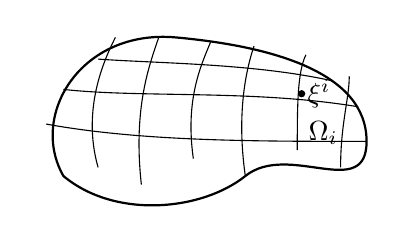
\begin{tikzpicture}[scale=1.1, >=stealth]
  \def\basepathB{
    (-1.4,-0.9) .. controls (-1.8,-0.2) and (-1.2,0.8) .. (-0.1,0.7)
    .. controls (1.0,0.6) and (2.1,0.3) .. (2.1,-0.5)
    .. controls (2.1,-1.2) and (1.2,-0.5) .. (0.7,-0.9)
    .. controls (0.2,-1.3) and (-0.8,-1.4) .. (-1.4,-0.9)
  }
  \draw[thick] \basepathB;

  % 内部网格线
  \draw (-1.0,-0.8) .. controls (-1.2,-0.1) and (-0.9,0.5) .. (-0.8,0.7);
  \draw (-0.5,-1.0) .. controls (-0.6,-0.1) and (-0.4,0.4) .. (-0.3,0.7);
  \draw (0.1,-0.7) .. controls (0.0,0.0) and (0.2,0.4) .. (0.3,0.65);
  \draw (0.7,-0.9) .. controls (0.6,-0.2) and (0.7,0.3) .. (0.8,0.6);
  \draw (1.3,-0.6) .. controls (1.3, -0.1) and (1.3,0.3) .. (1.4,0.5);
  \draw (1.8,-0.8) .. controls (1.8,-0.3) and (1.9,0.0) .. (1.9,0.25);

  \draw (-1.6,-0.3) .. controls (-0.5,-0.5) and (0.8,-0.5) .. (2.1,-0.5);
  \draw (-1.4,0.1) .. controls (-0.5,0.0) and (0.8,0.1) .. (2.0,-0.1);
  \draw (-1.0,0.45) .. controls (-0.3,0.4) and (0.8,0.4) .. (1.7,0.2);

  \node at (1.55, 0.05) {$\boldsymbol{\xi}^i$};
  \fill (1.35, 0.05) circle (1.2pt);
  \node at (1.6, -0.4) {$\Omega_i$};
\end{tikzpicture}
\caption{}\label{fig:10.1.2}
\end{minipage}
\end{figure}

对照一元函数积分的定义, 将 $[a, b]$ 分割成若干子区间, 计算这些区间的长度十分容易. 但是, 在 $\mathbb{R}^{2}$ 中, 一个点集 $\Omega$ 即使有界, 也可能相当复杂. 如何分割 $\Omega$, 如何确定面积 $v(\Omega_i)$, 这是建立二重积分精确定义的最大障碍. 为克服这些障碍, 我们分成两步: 首先讨论二维闭区间上的二重积分, 然后再讨论 $\mathbb{R}^{2}$ 中任一有界集上的二重积分.

\begin{definition}\label{def:10.1.1}
设 $I = [a, b] \times [c, d]$ 为 $\mathbb{R}^{2}$ 中的闭区间 (即每边平行于坐标轴的闭矩形 (闭长方形)). 作 $[a, b]$ 的分割
\[
  T_{x}\colon a = x_{0} < x_{1} < \cdots < x_{n} = b;
\]
又作 $[c, d]$ 的分割
\[
  T_{y}\colon c = y_{0} < y_{1} < \cdots < y_{m} = d.
\]
两族平行直线 $x = x_{i}\,(i = 0, 1, \cdots, n)$ 与 $y = y_{j}\,(j = 0, 1, \cdots, m)$ 将 $I$ 分割成 $k = n \times m$ 个子区间
\[
  [x_{i-1}, x_{i}] \times [y_{j-1}, y_{j}], \quad i = 1, \cdots, n;\; j = 1, \cdots, m.
\]
这 $k$ 个子区间的全体组成 $I$ 的一个分割 $T = T_x \times T_y = \{I_1, I_2, \cdots, I_k\}$. 任取 $\boldsymbol{\xi}^i \in I_i\, (i = 1, 2, \cdots, k)$. 对二元函数 $f\colon I \to \mathbb{R}$ 作 Riemann 和 (也称为积分和)
\[
  \sum_{i=1}^{k} f(\boldsymbol{\xi}^{i}) v(I_{i}),
\]
其中 $v(I_{i})$ 为二维闭区间 (闭矩形) $I_{i}$ 的面积, 即 $I_{i}$ 的长与宽之积. 记
\[
  \|T\| = \max\{\operatorname{diam}I_{1}, \operatorname{diam}I_{2}, \cdots, \operatorname{diam}I_{k}\},
\]
这里 $I_{i}$ 的直径 $\operatorname{diam}I_{i}$ 为矩形 $I_{i}$ 的对角线的长度. 称 $\|T\|$ 为分割 $T$ 的模或宽度. 称 $\boldsymbol{\xi} = (\boldsymbol{\xi}^{1}, \boldsymbol{\xi}^{2}, \cdots, \boldsymbol{\xi}^{k}) \in I_{1} \times I_{2} \times \cdots \times I_{k}$ 为上述 Riemann 和的值点向量, 称 $\boldsymbol{\xi}^{1}, \boldsymbol{\xi}^{2}, \cdots, \boldsymbol{\xi}^{k}$ 为值点.

如果 $\exists J \in \mathbb{R}$, s.t. $\forall \varepsilon > 0$, $\exists \delta > 0$, 当 $\|T\| < \delta$ 时, $\forall \boldsymbol{\xi} \in I_1 \times I_2 \times \cdots \times I_k$, 都有
\[
  \left|\sum_{i=1}^{k} f(\boldsymbol{\xi}^{i}) v(I_{i}) - J\right| < \varepsilon,
\]
则称二元函数 $f$ 在闭区间 $I$ 上 (Riemann) 可积, 而
\[
  J = \lim_{\|T\| \to 0} \sum_{i=1}^{k} f(\boldsymbol{\xi}^{i}) v(I_{i}) \reason{def} \iint_{I} f(x, y)\,\mathrm{d}x\mathrm{d}y \quad\text{或}\quad \int_{I} f\,\mathrm{d}v \quad\text{或}\quad \int_{I} f
\]
称为 $f$ 在 $I$ 上的二重积分, 或简称为 $f$ 在 $I$ 上的积分. 这里 $f$ 称为被积函数, $I$ 称为积分区间, $\mathrm{d}x\mathrm{d}y$ 与 $\mathrm{d}v$ 称为面积元.
\end{definition}

如此定义的积分具有与一元函数积分类似的简单性质.

\begin{theorem}\label{thm:10.1.1}
\begin{enumerate}
  \item $\displaystyle\int_{I} c = c v(I),\, c \in \mathbb{R}$;
  \item 设 $f$ 在二维闭区间 $I \subset \mathbb{R}^2$ 上可积, 则 $\forall c \in \mathbb{R}$ ($c$ 为常数), $cf$ 也可积, 且
  \[
    \int_{I} c f = c\int_{I} f.
  \]
  \item 设 $f_{1}$ 与 $f_{2}$ 在 $I$ 上都可积, 则 $f_{1} + f_{2}$ 在 $I$ 上也可积, 且
  \[
    \int_{I}(f_{1}+f_{2}) = \int_{I} f_{1} + \int_{I} f_{2}.
  \]
  \item 设 $f \geqslant 0$ 且在 $I$ 上可积, 则 $\displaystyle\int_{I} f \geqslant 0$. 特别地, 如果 $f_{1}, f_{2}$ 都在 $I$ 上可积, 且 $f_{1} \geqslant f_{2}$, 则 $\displaystyle\int_{I} f_{1} \geqslant \int_{I} f_{2}$.
  \item 设 $f$ 在 $I$ 上可积, 则 $|f|$ 在 $I$ 上也可积, 且
  \[
    \left|\int_{I} f\right| \leqslant \int_{I} |f|.
  \]
\end{enumerate}
\end{theorem}

\begin{proof}
(1) 因为
\[
  \sum_{i=1}^{k} c v(I_{i}) = c \sum_{i=1}^{k} v(I_{i}) = c v(I),
\]
所以根据积分定义知 $\displaystyle\int_{I} c = c v(I)$.

(2) 因为
\[
  \sum_{i=1}^{k} c f(\boldsymbol{\xi}^{i}) v(I_{i}) = c \sum_{i=1}^{k} f(\boldsymbol{\xi}^{i}) v(I_{i}),
\]
所以根据积分定义知 $\displaystyle\int_{I} c f = c\int_{I} f$.

(3) 因为
\[
  \sum_{i=1}^{k}(f_{1}+f_{2})(\boldsymbol{\xi}^{i}) v(I_{i}) = \sum_{i=1}^{k} f_{1}(\boldsymbol{\xi}^{i}) v(I_{i}) + \sum_{i=1}^{k} f_{2}(\boldsymbol{\xi}^{i}) v(I_{i}),
\]
所以根据积分定义知 $\displaystyle\int_{I}(f_{1}+f_{2}) = \int_{I} f_{1} + \int_{I} f_{2}$.

(4) 因为 $\displaystyle\sum_{i=1}^{k} f(\boldsymbol{\xi}^{i}) v(I_{i}) \geqslant 0$, 故必有 $\displaystyle\int_{I} f \geqslant 0$. (反证) 假设 $\displaystyle\int_{I} f < 0$, 取 $\varepsilon_{0} = -\dfrac{1}{2}\int_{I} f > 0$, 根据 $f$ 可积与积分定义知, $\exists \delta > 0$, 当 $\|T\| < \delta$ 时, 有
\[
  0 \leqslant \sum_{i=1}^{k} f(\boldsymbol{\xi}^{i}) v(I_{i}) < \int_{I} f + \varepsilon_{0} = \int_{I} f - \frac{1}{2}\int_{I} f = \frac{1}{2}\int_{I} f < 0,
\]
矛盾.

特别地, 当 $f_{1} \geqslant f_{2}$ 时, $f_{1} - f_{2} \geqslant 0$. 由上得到
\[
  \int_{I} f_{1} - \int_{I} f_{2} = \int_{I}(f_{1}-f_{2}) \geqslant 0 \implies \int_{I} f_{1} \geqslant \int_{I} f_{2}.
\]

(5) 类似\extref{例 6.1.9} 应用\cref{thm:10.1.7}的 (3) 或 (8) 知, $f$ 可积蕴涵着 $|f|$ 可积. 再由 $-|f| \leqslant f \leqslant |f|$ 及 (4) 立得
\[
  -\int_{I} |f| \leqslant \int_{I} f \leqslant \int_{I} |f|, \quad \text{即} \quad \left|\int_{I} f\right| \leqslant \int_{I} |f|. \qedhere
\]
\end{proof}

\begin{theorem}[惟一性]\label{thm:10.1.2}
设 $f$ 在闭区间 $I = [a, b] \times [c, d]$ 上可积, 则积分值 $J = \displaystyle\int_{I} f$ 是惟一的.
\end{theorem}

\begin{proof}
仿照\extref{定理 6.1.1}证明.
\end{proof}

\begin{theorem}[可积的必要条件]\label{thm:10.1.3}
设 $f$ 在闭区间 $I = [a, b] \times [c, d]$ 上可积, 则 $f$ 在 $I$ 上有界 (因而无界函数不是可积的). 但反之不真.
\end{theorem}

\begin{proof}
仿照\extref{定理 6.1.2}的证明. 只需将反例改为
\[
  f(x, y) = D(x, y) = \begin{cases}
    1, & (x, y) \in \mathbb{Q}^{2} \cap [0, 1]^{2}, \\
    0, & (x, y) \in [0, 1]^{2} \setminus \mathbb{Q}^{2}.
  \end{cases} \qedhere
\]
\end{proof}

与一元函数一样, \cref{thm:10.1.3}只是可积的必要条件, 它只能否定无界函数是可积的, 但对有界函数是否可积就束手无策了. 要判断一个函数是否可积, 原则上可以根据定义直接考察 Riemann 和是否无限接近某个常数 $J$. 但由于常数 $J$ 不易预知及 Riemann 和的复杂性, 这种判断是非常困难的.

为给出 $f$ 在 $I = [a, b] \times [c, d]$ 上可积的充要条件, 先引进零面积集、零测集的概念.

\begin{definition}\label{def:10.1.2}
设 $A \subset \mathbb{R}^{2}$. 如果对任何 $\varepsilon > 0$, 存在有限个闭区间 $I_{1}, I_{2}, \cdots, I_{k}$ 使得 $\bigcup\limits_{i=1}^{k} I_{i} \supseteq A$, 且 $\sum\limits_{i=1}^{k} v(I_{i}) < \varepsilon$, 则称 $A$ 为\textbf{零面积集}.

设 $A \subset \mathbb{R}^{2}$. 如果对任何 $\varepsilon > 0$, 存在至多可数个二维闭区间 $I_{1}, I_{2}, \cdots, I_{k}, \cdots$, 使得 $\bigcup\limits_{i=1}^{\infty} I_{i} \supseteq A$, 且 $\sum\limits_{i=1}^{\infty} v(I_{i}) < \varepsilon$, 则称 $A$ 为\textbf{零测集}.
\end{definition}

该定义中将「闭区间」改为「开区间」, 或「闭圆」, 或「开圆」都是等价的.

\begin{theorem}\label{thm:10.1.4}
零面积集必为零测集, 但反之不真.
\end{theorem}

\begin{proof}
如果 $A \subset \mathbb{R}^{2}$ 为零面积集, 则对任何 $\varepsilon > 0$, 必有二维闭区间 $I_{1}, I_{2}, \cdots, I_{k}$ 使 $\bigcup\limits_{i=1}^{k} I_{i} \supset A$, 且 $\sum\limits_{i=1}^{k} v(I_{i}) < \varepsilon$. 再选面积充分小的 $I_{k+1}, I_{k+2}, \cdots$, 使 $\sum\limits_{i=1}^{\infty} v(I_{i}) < \varepsilon$. 而 $\bigcup\limits_{i=1}^{\infty} I_{i} \supset \bigcup\limits_{i=1}^{k} I_{i} \supset A$ 是显然的. 因此, $A$ 为零测集.

\textbf{反例}: $[0, 1]^{2}$ 中有理点的全体 $\mathbb{Q}^{2} \cap [0, 1]^{2} = \{P^{i} \mid i \in \mathbb{Z}_{+}\}$ 为零测集, 但非零面积集. 作以 $P_i$ 为中心, $\dfrac{\sqrt{\varepsilon}}{2^i}$ 为边长的正方形 $I_i$, 则
\[
  \bigcup_{i=1}^{\infty} I_i \supset \bigcup_{i=1}^{\infty} \{P^i\} = \mathbb{Q}^{2} \cap [0, 1]^{2},
\]
且
\[
  \sum_{i=1}^{\infty} v(I_i) = \sum_{i=1}^{\infty} \left(\frac{\sqrt{\varepsilon}}{2^i}\right)^2 = \sum_{i=1}^{\infty} \frac{\varepsilon}{2^{2i}} = \sum_{i=1}^{\infty} \left(\frac{1}{4}\right)^i \varepsilon = \frac{\varepsilon}{3} < \varepsilon.
\]
由此推得 $\mathbb{Q}^{2} \cap [0, 1]^{2}$ 为零测集. 但它为非零面积集. (反证) 假设 $\mathbb{Q}^{2} \cap [0, 1]^{2}$ 为零面积集, 则对 $\varepsilon_0 = \dfrac{1}{2}$ 存在闭区间 $I_1, I_2, \cdots, I_k$ 使得 $\bigcup\limits_{i=1}^{k} I_i \supset \mathbb{Q}^{2} \cap [0, 1]^{2}$, 且 $\sum\limits_{i=1}^{k} v(I_i) < \varepsilon_0 = \dfrac{1}{2}$. 显然,
\[
  [0, 1]^{2} = \overline{\mathbb{Q}^{2} \cap [0, 1]^{2}} \subset \overline{\bigcup_{i=1}^{k} I_i} = \bigcup_{i=1}^{k} \overline{I_i} = \bigcup_{i=1}^{k} I_i,
\]
所以
\[
  1 = v([0, 1]^{2}) \leqslant v\left(\bigcup_{i=1}^{k} I_i\right) \leqslant \sum_{i=1}^{k} v(I_i) < \varepsilon_0 = \frac{1}{2},
\]
矛盾.
\end{proof}

\begin{example}\label{ex:10.1.1}
设 $f\colon [a, b] \to \mathbb{R}$ 为连续函数, 则集合 ($f$ 的图像)
\[
  \operatorname{graph} f = \{(x, f(x)) \mid x \in [a, b]\} \subset \mathbb{R}^{2}
\]
为零面积集.
\end{example}

\begin{proof}
任给 $\varepsilon > 0$, 因 $f$ 在 $[a, b]$ 上连续, 故一致连续. 于是, 存在 $[a, b]$ 的一个分割: $a = x_{0} < x_{1} < \cdots < x_{n} = b$, 当 $t_{1}, t_{2} \in [x_{i-1}, x_{i}]\, (i = 1, 2, \cdots, n)$ 时,
\[
  |f(t_{1}) - f(t_{2})| < \frac{\varepsilon}{b - a}.
\]
令 $m_{i} = \min f([x_{i-1}, x_{i}])$, $M_{i} = \max f([x_{i-1}, x_{i}])$, 则
\[
  0 \leqslant M_{i} - m_{i} < \frac{\varepsilon}{b - a}, \quad i = 1, 2, \cdots, n.
\]
设 $I_{i} = [x_{i-1}, x_{i}] \times [m_{i}, M_{i}]\, (i = 1, 2, \cdots, n)$. 显见 (\cref{fig:10.1.3}), $\operatorname{graph} f \subset \bigcup\limits_{i=1}^{n} I_{i}$, 且
\[
  \sum_{i=1}^{n} v(I_{i}) < \sum_{i=1}^{n}(x_{i} - x_{i-1}) \cdot \frac{\varepsilon}{b - a} = (b - a) \cdot \frac{\varepsilon}{b - a} = \varepsilon.
\]
因此, $\operatorname{graph} f$ 为零面积集.
\end{proof}

\begin{figure}[htbp]
\centering
\begin{tikzpicture}[scale=1.15, >=stealth]
  % 坐标轴
  \draw[->, thick] (-0.3,0) -- (6.0,0) node[below] {$x$};
  \draw[->, thick] (0,-0.3) -- (0,4.2) node[left] {$y$};

  % 各个竖直立柱的侧边界
  \draw[thick] (0.8,0) -- (0.8,2.0);
  \draw[thick] (1.7,0) -- (1.7,2.0);
  \draw[thick] (2.6,0) -- (2.6,2.2);
  \draw[thick] (3.5,0) -- (3.5,2.7);
  \draw[thick] (4.5,0) -- (4.5,3.6);
  \draw[thick] (5.4,0) -- (5.4,3.6);

  % 绘制每个柱体顶部的矩形 I_i [m_i, M_i] 并填充斜线阴影
  \fill[pattern=north east lines] (0.8,1.8) rectangle (1.7,2.0);
  \draw[thick] (0.8,1.8) rectangle (1.7,2.0);

  \fill[pattern=north east lines] (1.7,1.7) rectangle (2.6,1.9);
  \draw[thick] (1.7,1.7) rectangle (2.6,1.9);

  \fill[pattern=north east lines] (2.6,1.8) rectangle (3.5,2.2);
  \draw[thick] (2.6,1.8) rectangle (3.5,2.2);

  \fill[pattern=north east lines] (3.5,2.1) rectangle (4.5,2.7);
  \draw[thick] (3.5,2.1) rectangle (4.5,2.7);

  \fill[pattern=crosshatch] (4.5,2.6) rectangle (5.4,3.6);
  \draw[thick] (4.5,2.6) rectangle (5.4,3.6);

  % 函数曲线 y = f(x)
  \draw[very thick] (0.8,1.95) .. controls (1.2,1.82) and (1.5,1.75) .. (2.1,1.72)
    .. controls (2.6,1.75) and (3.0,1.95) .. (3.5,2.18)
    .. controls (4.0,2.4) and (4.3,2.6) .. (4.5,2.8)
    .. controls (4.8,3.1) and (5.2,3.4) .. (5.4,3.55);

  % 指向其中一个小矩形 I_i 的箭头
  \draw[->] (2.7, 3.2) node[above left] {$I_i$} -- (3.8, 2.5);
\end{tikzpicture}
\caption{}\label{fig:10.1.3}
\end{figure}

\begin{example}\label{ex:10.1.2}
设 $l \subset \mathbb{R}^{2}$ 为 $C^{1}$ 参数曲线, 则 $l$ 为零面积集.

更进一步, 设 $l \subset \mathbb{R}^{2}$ 为 $C^{0}$ 参数曲线, 并且其中至少有一个分量有连续的导数, 则 $l$ 为零面积集.
\end{example}

\begin{proof}
设 $l$ 有参数表示 $(x, y) = (x(t), y(t)),\, t \in [\alpha, \beta]$, 其中 $x$ 与 $y$ 为 $[\alpha, \beta]$ 上的连续函数, 不妨再设 $y$ 在 $[\alpha, \beta]$ 上有连续的导数. 由最值定理, $\exists M > 0$, s.t. $|y'(t)| \leqslant M$, $\forall t \in [\alpha, \beta]$. 于是, $\forall \varepsilon > 0$, 由于 $x(t)$ 在 $[\alpha, \beta]$ 上一致连续, 故必有分割
\[
  T\colon \alpha = t_{0} < t_{1} < \cdots < t_{m} = \beta,
\]
s.t. 当 $s, t \in [t_{i-1}, t_i]\, (i = 1, 2, \cdots, m)$ 时, 有
\[
  |x(s) - x(t)| < \frac{\varepsilon}{2M(\beta - \alpha)}.
\]
令
\[
  a_{i} = \min x([t_{i-1}, t_{i}]), \quad b_{i} = \max x([t_{i-1}, t_{i}]),
\]
则有 $b_{i} - a_{i} \leqslant \dfrac{\varepsilon}{2M(\beta - \alpha)}$. 再令
\[
  c_{i} = \min y([t_{i-1}, t_{i}]), \quad d_{i} = \max y([t_{i-1}, t_{i}]),
\]
\[
  I_{i} = [a_{i}, b_{i}] \times [c_{i}, d_{i}], \quad i = 1, 2, \cdots, m.
\]
于是, 当 $t \in [t_{i-1}, t_i]$ 时, $(x(t), y(t)) \in I_i\, (i = 1, 2, \cdots, m)$. 所以
\[
  l \subset \bigcup_{i=1}^{m} I_{i}.
\]
由于 $y(t)$ 在 $[\alpha, \beta]$ 上连续, 根据最值定理, $\exists t_{i}^{(0)}, t_{i}^{(1)} \in [t_{i-1}, t_{i}]$, s.t. $y(t_{i}^{(0)}) = d_{i}$, $y(t_{i}^{(1)}) = c_{i}$. 再由 Lagrange 中值定理, $\exists \theta_{i} \in [t_{i}^{(0)}, t_{i}^{(1)}] \subset [t_{i-1}, t_{i}]$, 有
\begin{align*}
  0 &\leqslant d_{i} - c_{i} = y(t_{i}^{(0)}) - y(t_{i}^{(1)}) = y'(\theta_{i})(t_{i}^{(0)} - t_{i}^{(1)}) \\
    &\leqslant M |t_{i}^{(0)} - t_{i}^{(1)}| \leqslant M(t_{i} - t_{i-1}).
\end{align*}
由此推得
\begin{align*}
  \sum_{i=1}^{m} v(I_{i}) &= \sum_{i=1}^{m}(b_{i} - a_{i})(d_{i} - c_{i}) \leqslant \sum_{i=1}^{m} \frac{\varepsilon}{2M(\beta - \alpha)} M(t_{i} - t_{i-1}) \\
  &= \frac{\varepsilon}{2M(\beta - \alpha)} M(\beta - \alpha) = \frac{\varepsilon}{2} < \varepsilon.
\end{align*}
这就证明了 $l$ 为零面积集.
\end{proof}

\begin{remark}\label{rem:10.1.1}
\begin{enumerate}
  \item 设函数 $f\colon [a, b] \to \mathbb{R}$ 连续, 由\cref{ex:10.1.2}的结论知, $f$ 的图像
  \[
    \operatorname{graph} f = \{(x, f(x)) \mid x \in [a, b]\} = \{(t, f(t)) \mid t \in [a, b]\} \subset \mathbb{R}^{2}
  \]
  为零面积集.
  \item 如果 $x(t), y(t)$ 只连续, 但都不具有连续可导的条件, 则\cref{ex:10.1.2}的结论可能不成立. 甚至我们将在第三册中给出一条连续的参数曲线, 它竟能充满整个正方形, 从而这条连续曲线就不是零面积集.
\end{enumerate}
\end{remark}

关于零面积集与零测集, 还有下面定理.

\begin{theorem}\label{thm:10.1.5}
\begin{enumerate}
  \item 至多可数集为零测集.
  \item 零测集的任何子集为零测集.
  \item 至多可数个零测集 $A_i$ 的并集 $\bigcup\limits_{i} A_i$ 仍为零测集.
  \item 零面积集的任何子集为零面积集.
  \item 有限个零面积集之并仍为零面积集; 可数个零面积集之并未必为零面积集.
  \item $A$ 为零面积集 $\iff \overline{A}$ 也为零面积集.
  \item 如果 $A$ 为有界闭集, 则 $A$ 为零测集 $\iff A$ 为零面积集.
\end{enumerate}
\end{theorem}

\begin{proof}
(1) $\sim$ (4) 和 (5) 的第一结论是显而易见的, 读者自己可以证明. 这里只证 (5) 的第二个论断及 (6), (7).

(5) $\boldsymbol{x} = (x, y) \in \mathbb{R}^{2}$, $\forall \varepsilon > 0$, 作闭区间
\[
  I = \left[x - \frac{\sqrt{\varepsilon}}{4}, x + \frac{\sqrt{\varepsilon}}{4}\right] \times \left[y - \frac{\sqrt{\varepsilon}}{4}, y + \frac{\sqrt{\varepsilon}}{4}\right],
\]
则 $\boldsymbol{x} \in I$, 且 $v(I) = \left(\dfrac{\sqrt{\varepsilon}}{2}\right)^{2} = \dfrac{\varepsilon}{4} < \varepsilon$. 因此, 独点集 $\{\boldsymbol{x}\}$ 为零面积集.

显然, $\mathbb{Q}^2 \cap [0, 1]^2 = \{P^i \mid i \in \mathbb{Z}_+\}$ 为可数个独点集之并, 因而它为可数个零面积集的并. 但根据\cref{thm:10.1.4}证明知, $\mathbb{Q}^2 \cap [0, 1]^2$ 为非零面积集.

(6) ($\Leftarrow$) 因为 $A \subset \overline{A}$, 根据 (4) 知, $\overline{A}$ 为零面积集蕴涵着 $A$ 为零面积集.

($\Rightarrow$) 设 $A$ 为零面积集, 则 $\forall \varepsilon > 0$, 必有闭区间 $I_{1}, I_{2}, \cdots, I_{m}$, s.t.
\[
  A \subset \bigcup_{i=1}^{m} I_{i}, \quad \sum_{i=1}^{m} v(I_{i}) < \varepsilon.
\]
由于 $\bigcup\limits_{i=1}^{m} I_{i}$ 为闭集, 所以仍有
\[
  \overline{A} \subset \overline{\bigcup_{i=1}^{m} I_{i}} = \bigcup_{i=1}^{m} \overline{I_{i}} = \bigcup_{i=1}^{m} I_{i}.
\]
由此可见 $\overline{A}$ 为零面积集.

(7) ($\Leftarrow$) 见\cref{thm:10.1.4}.

($\Rightarrow$) 设 $A$ 为紧致的零测集, 则对任何 $\varepsilon > 0$, 存在开区间序列 $\{I_{i}\}$, 使得
\[
  A \subset \bigcup_{i=1}^{\infty} I_{i} \quad\text{且}\quad \sum_{i=1}^{\infty} v(I_{i}) < \varepsilon.
\]
由有限覆盖定理, 从 $\{I_{i}\}$ 中可选出有限个开区间仍能覆盖住 $A$, 这些开区间面积之和自然仍小于 $\varepsilon$, 所以 $A$ 为零面积集.
\end{proof}

下面将给出 Riemann 可积的充要条件, 它只与被积函数 $f$ 本身有关, 而不涉及 Riemann 积分的值.

设 $f\colon I \to \mathbb{R}$ 为有界函数, $I = [a, b] \times [c, d] \subset \mathbb{R}^2$ 为闭区间, $M = \sup\limits_{\boldsymbol{x} \in I} f(\boldsymbol{x})$, $m = \inf\limits_{\boldsymbol{x} \in I} f(\boldsymbol{x})$. $T = \{I_1, I_2, \cdots, I_k\}$ 为\cref{def:10.1.1}中所述的 $I$ 的一个分割.
\[
  M_{i}^{f} = \sup_{\boldsymbol{x} \in I_{i}} f(\boldsymbol{x}), \quad m_{i}^{f} = \inf_{\boldsymbol{x} \in I_{i}} f(\boldsymbol{x}).
\]
在不致混淆时, 记 $M_{i}^{f}$ 为 $M_{i}$, $m_{i}^{f}$ 为 $m_{i}$.

分别称
\[
  S(T, f) = \sum_{i=1}^{k} M_{i} v(I_{i}) \quad\text{与}\quad s(T, f) = \sum_{i=1}^{k} m_{i} v(I_{i})
\]
为 $f$ 关于分割 $T$ 的 Darboux 上和与 Darboux 下和, 统称为 Darboux 和. 在不致混淆时, 分别记 $S(T, f)$ 与 $s(T, f)$ 为 $S(T)$ 与 $s(T)$. 显然, $\forall \boldsymbol{\xi}^{i} \in I_{i}\,(i = 1, 2, \cdots, k)$, Riemann 和 $S(T, f, \boldsymbol{\xi}) = \sum\limits_{i=1}^{k} f(\boldsymbol{\xi}^{i}) v(I_{i})$ 满足
\[
  m v(I) \leqslant \sum_{i=1}^{k} m_{i} v(I_{i}) \leqslant \sum_{i=1}^{k} f(\boldsymbol{\xi}^{i}) v(I_{i}) \leqslant \sum_{i=1}^{k} M_{i} v(I_{i}) \leqslant M v(I),
\]
即
\[
  m v(I) \leqslant s(T, f) \leqslant S(T, f, \boldsymbol{\xi}) \leqslant S(T, f) \leqslant M v(I),
\]
其中 $\boldsymbol{\xi} = (\boldsymbol{\xi}^{1}, \boldsymbol{\xi}^{2}, \cdots, \boldsymbol{\xi}^{k})$.

设 $\omega_{i}^{f} = M_{i}^{f} - m_{i}^{f}$, 称它为 $f$ 在 $I_{i}$ 上的振幅, 简记为 $\omega_{i} = M_{i} - m_{i}$, 而
\[
  S(T, f) - s(T, f) = \sum_{i=1}^{k}(M_{i} - m_{i}) v(I_{i}) = \sum_{i=1}^{k} \omega_{i} v(I_{i}) \quad \left(\text{或}\quad \sum_{T} \omega_{i} v(I_{i})\right)
\]
称为 $f$ 在 $I$ 上关于分割 $T$ 的振幅和.

\begin{lemma}\label{lem:10.1.1}
对闭区间 $I \subset \mathbb{R}^2$ 的同一分割 $T = \{I_1, I_2, \cdots, I_k\}$, 相对于任何 $\boldsymbol{\xi} = (\boldsymbol{\xi}^1, \boldsymbol{\xi}^2, \cdots, \boldsymbol{\xi}^k) \in I_1 \times I_2 \times \cdots \times I_k$, 有
\[
  S(T, f) = \sup_{\boldsymbol{\xi}} \sum_{i=1}^{k} f(\boldsymbol{\xi}^{i}) v(I_{i}), \quad s(T, f) = \inf_{\boldsymbol{\xi}} \sum_{i=1}^{k} f(\boldsymbol{\xi}^{i}) v(I_{i}).
\]
\end{lemma}

\begin{proof}
仿\extref{引理 6.1.1}证明.
\end{proof}

设 $T' = T_{x}' \times T_{y}'$, $T'' = T_{x}'' \times T_{y}''$ 为闭区间 $I \subset \mathbb{R}^2$ 的两个分割. $T_{x}' + T_{x}''$ 表示将 $T'_{x}$ 与 $T''_{x}$ 的所有分点合并得到的分割 (重复的分点只取一次), $T'_{y} + T''_{y}$ 表示将 $T'_{y}$ 与 $T''_{y}$ 的所有分点合并得到的分割 (重复的分点只取一次). 记 $T' + T'' = (T_{x}' + T''_{x}) \times (T'_{y} + T''_{y})$.

\begin{lemma}\label{lem:10.1.2}
$S(T' + T'') \leqslant S(T')$, $s(T' + T'') \geqslant s(T')$;
\[
  S(T' + T'') \leqslant S(T''), \quad s(T' + T'') \geqslant s(T'').
\]
\end{lemma}

\begin{proof}
类似\extref{引理 6.1.2}的证明知, 分割增加新分点后, 上和不增, 下和不减. 因此, 立即推得引理中的结论.
\end{proof}

\begin{lemma}\label{lem:10.1.3}
对闭区间 $I \subset \mathbb{R}^{2}$ 的任意两个分割 $T'$ 与 $T''$, 有
\[
  s(T') \leqslant S(T'').
\]
\end{lemma}

\begin{proof}
由\cref{lem:10.1.2}便有
\[
  s(T') \leqslant s(T' + T'') \leqslant S(T' + T'') \leqslant S(T''). \qedhere
\]
\end{proof}

\begin{lemma}\label{lem:10.1.4}
$m v(I) \leqslant \sup\limits_{T'} s(T') \leqslant \inf\limits_{T''} S(T'') \leqslant M v(I)$.
\end{lemma}

\begin{proof}
由\cref{lem:10.1.3}知
\[
  m v(I) \leqslant s(T') \leqslant S(T'') \leqslant M v(I),
\]
从而有
\[
  m v(I) \leqslant \sup_{T'} s(T') \leqslant \inf_{T''} S(T'') \leqslant M v(I),
\]
即
\[
  m v(I) \leqslant s \leqslant S \leqslant M v(I),
\]
其中 $S = \inf\limits_{T} S(T)$ 与 $s = \sup\limits_{T} s(T)$ 分别称为 $f$ 在 $I$ 上的上积分与下积分.
\end{proof}

\begin{theorem}[Darboux 定理]\label{thm:10.1.6}
$\lim\limits_{\|T\| \to 0} S(T) = S, \quad \lim\limits_{\|T\| \to 0} s(T) = s$.
\end{theorem}

\begin{proof}
$\forall \varepsilon > 0$, 由 $S$ 的定义知, 必有某个分割 $T' = T_{x}' \times T_{y}'$, s.t.
\[
  S(T') < S + \frac{\varepsilon}{2}.
\]
设 $T_{x}'$ 与 $T_{y}'$ 分别由 $p$ 个与 $q$ 个分点构成. 对于任意另外一个分割 $T$, $(T+T')_{x}$ 至多比 $T_{x}$ 多 $p$ 个分点, $(T+T')_{y}$ 至多比 $T_{y}$ 多 $q$ 个分点. 根据\extref{引理 6.1.2}证明中的方法与\cref{lem:10.1.2}有
\begin{align*}
  S(T) - (M - m)[p(d - c) + q(b - a)] \|T\|
  &\leqslant S(T) - (M - m)[p(d - c)\|T_{x}\| + q(b - a)\|T_{y}\|] \\
  &\leqslant S(T + T') \leqslant S(T').
\end{align*}
于是, 当 $\|T\| < \dfrac{\varepsilon}{2(M - m + 1)[p(d - c) + q(b - a)]}$ 时,
\begin{align*}
  S &\leqslant S(T) \leqslant S(T') + (M - m)[p(d - c) + q(b - a)] \|T\| \\
    &< S(T') + (M - m)[p(d - c) + q(b - a)] \frac{\varepsilon}{2(M - m + 1)[p(d - c) + q(b - a)]} \\
    &< S(T') + \frac{\varepsilon}{2} < \left(S + \frac{\varepsilon}{2}\right) + \frac{\varepsilon}{2} = S + \varepsilon.
\end{align*}
这就证明了 $\lim\limits_{\|T\| \to 0} S(T) = S$.

同理, 或用 $-f$ 代替 $f$ 得到 $\lim\limits_{\|T\| \to 0} s(T) = s$.
\end{proof}

\begin{theorem}[Riemann 可积的充要条件]\label{thm:10.1.7}
设 $I \subset \mathbb{R}^2$ 为闭区间, $f\colon I \to \mathbb{R}$ 为有界函数, 即 $|f(\boldsymbol{x})| \leqslant M$, $\forall \boldsymbol{x} \in I$. 则下面结论等价:
\begin{enumerate}
  \item $f$ 在 $I$ 上 Riemann 可积.
  \item $f$ 在 $I$ 上的上积分与下积分相等, 即 $S = s$.
  \item 对任何 $\varepsilon > 0$, 存在 $I$ 的某个分割 $T$, 使得
  \[
    S(T) - s(T) = \sum_{i=1}^{k} \omega_{i} v(I_{i}) < \varepsilon.
  \]
  \item 存在 $I$ 的分割串 $T_{m}\,(m = 1, 2, \cdots)$, 使得
  \[
    \lim_{m \to +\infty}[S(T_{m}) - s(T_{m})] = 0.
  \]
  \item $\lim\limits_{\|T\| \to 0}[S(T) - s(T)] = 0$.
  \item 对任何 $\varepsilon > 0$, 存在 $I$ 的某个分割 $T$, 使对任何 $\boldsymbol{\xi} = (\boldsymbol{\xi}^{1}, \boldsymbol{\xi}^{2}, \cdots, \boldsymbol{\xi}^{k}) \in I_{1} \times I_{2} \times \cdots \times I_{k}$, 有
  \[
    |S(T, f, \boldsymbol{\xi}) - J| < \varepsilon.
  \]
  \item 对任何 $\varepsilon > 0, \eta > 0$, 存在 $I$ 的某个分割 $T = \{I_{1}, I_{2}, \cdots, I_{k}\}$, 使得
  \[
    \sum_{\omega_{i} \geqslant \varepsilon} v(I_{i}) < \eta.
  \]
  \item \textbf{(Lebesgue 定理)} $f$ 在 $I$ 上几乎处处连续, 即 $f$ 的不连续点集 $D_{\text{不}}^{f}$ (简记为 $D_{\text{不}}$) 为零测集, 记作
  \[
    \operatorname{meas} D_{\text{不}} = 0.
  \]
\end{enumerate}
\end{theorem}

\begin{proof}
我们只证 (3) $\Leftrightarrow$ (8), 其余证明完全仿照\extref{定理 6.1.4}中相应部分的证明.

(3) $\Rightarrow$ (8): 对任何 $\varepsilon > 0$, 存在 $I$ 的某分割 $T = \{I_{1}, I_{2}, \cdots, I_{k}\}$, 使得
\[
  S(T) - s(T) < \frac{\delta}{2} \varepsilon,
\]
其中 $\delta > 0$ 为任何正数. 令
\[
  D_{\delta} = \left\{\boldsymbol{x} \in I \;\middle|\; \omega_{f}(\boldsymbol{x}) = \lim_{r \to 0^{+}} \omega_{f}(\boldsymbol{x}, r) = \lim_{r \to 0^{+}} [\sup f(I \cap B(\boldsymbol{x}; r)) - \inf f(I \cap B(\boldsymbol{x}; r))] \geqslant \delta\right\},
\]
则
\[
  \sum_{D_{\delta} \cap I_{i}^{\circ} \neq \varnothing} v(I_{i}) < \frac{\varepsilon}{2}.
\]
若不然,
\[
  \frac{\delta}{2}\varepsilon > S(T) - s(T) \geqslant \sum_{D_{\delta} \cap I_{i}^{\circ} \neq \varnothing} \omega_{i} v(I_{i}) \geqslant \sum_{D_{\delta} \cap I_{i}^{\circ} \neq \varnothing} \delta v(I_{i}) \geqslant \delta \cdot \frac{\varepsilon}{2} = \frac{\delta}{2}\varepsilon,
\]
矛盾.

显然, $\bigcup\limits_{i=1}^{k} \partial I_{i}$ 为零面积集, 故必有闭区间 $J_{1}, J_{2}, \cdots, J_{m}$, 使得
\[
  \bigcup_{i=1}^{k} \partial I_{i} \subset \bigcup_{j=1}^{m} J_{j}, \quad\text{且}\quad \sum_{j=1}^{m} v(J_{j}) < \frac{\varepsilon}{2}.
\]
由此可知
\[
  D_{\delta} \subset \left(\bigcup_{\omega_{i} \geqslant \delta} I_{i}\right) \bigcup \left(\bigcup_{j=1}^{m} J_{j}\right),
\]
并且
\[
  \sum_{\omega_{i} \geqslant \delta} v(I_{i}) + \sum_{j=1}^{m} v(J_{j}) < \frac{\varepsilon}{2} + \frac{\varepsilon}{2} = \varepsilon.
\]
这就证明了 $D_{\delta}$ 为零测集, 从而由下面的\cref{thm:10.1.8}与\cref{thm:10.1.5}(3) 知, $D_{\text{不}} = \bigcup\limits_{n=1}^{\infty} D_{\frac{1}{n}}$ 为零测集.

(8) $\Rightarrow$ (3): 设 $D_{\text{不}}$ 为零测集. $\forall \varepsilon > 0$, 存在开区间序列 $\{U_{i}\}$, 使得
\[
  D_{\text{不}} \subset \bigcup_{i=1}^{\infty} U_{i}, \quad \sum_{i=1}^{\infty} v(U_{i}) < \frac{\varepsilon}{4M + 1}.
\]
对任何 $\boldsymbol{x} \in I \setminus \bigcup\limits_{i=1}^{\infty} U_{i} \subset I \setminus D_{\text{不}}$, $f$ 在 $\boldsymbol{x}$ 处连续, 故存在 $\boldsymbol{x}$ 的开邻域 $U_{\boldsymbol{x}}$, 使得 $\omega_{f}(U_{\boldsymbol{x}} \cap I) < \dfrac{\varepsilon}{2 v(I)}$.

显然 $\mathcal{J} = \left\{U_{i}, U_{\boldsymbol{x}} \;\middle|\; i = 1, 2, \cdots;\; \boldsymbol{x} \in I \setminus \bigcup\limits_{i=1}^{\infty} U_{i}\right\}$ 为紧致集 $I$ 的一个开覆盖. 根据 Heine-Borel 有限覆盖定理, 存在 $\mathcal{J}$ 的有限子集 $\mathcal{J}' = \{U_{i_{l}}, U_{\boldsymbol{x}^{s}} \mid l = 1, 2, \cdots, p;\; s = 1, 2, \cdots, q\}$ 覆盖 $I$. 再根据 Lebesgue 数定理, 存在 Lebesgue 数 $\lambda = \lambda(\mathcal{J}') > 0$. 当 $I$ 的分割 $T = \{I_{1}, I_{2}, \cdots, I_{k}\}$ 满足 $\|T\| < \lambda$ 时, 必有
\[
  I_{i} \subset U_{i_{l}} \quad\text{或}\quad U_{\boldsymbol{x}^{s}}.
\]
于是
\begin{align*}
  0 &\leqslant S(T) - s(T) = \sum_{i=1}^{k} \omega_{i} v(I_{i}) \\
    &\leqslant \sum_{I_{i} \subset U_{i_{l}}} \omega_{i} v(I_{i}) + \sum_{I_{i} \subset U_{\boldsymbol{x}^{s}}} \omega_{i} v(I_{i}) \\
    &\leqslant 2M \sum_{1} v(I_{i}) + \frac{\varepsilon}{2 v(I)} \sum_{2} v(I_{i}) \\
    &\leqslant 2M \sum_{i=1}^{\infty} v(U_{i}) + \frac{\varepsilon}{2 v(I)} v(I) \\
    &< 2M \cdot \frac{\varepsilon}{4M + 1} + \frac{\varepsilon}{2} < \varepsilon. \qedhere
\end{align*}
\end{proof}

\begin{remark}\label{rem:10.1.2}
我们可以不应用 Darboux 定理证明\cref{thm:10.1.7}中的 (2) $\Rightarrow$ (3).

事实上, 设 $J = S = s$. 由下积分的定义, 对任何 $\varepsilon > 0$, 存在闭区间 $I$ 的一个分割 $T'$, 使得
\[
  s(T') > J - \frac{\varepsilon}{2};
\]
又由上积分的定义, 存在闭区间 $I$ 的一个分割 $T''$, 使得
\[
  S(T'') < J + \frac{\varepsilon}{2}.
\]
于是, 有
\[
  J - \frac{\varepsilon}{2} < s(T') \leqslant s(T' + T'') \leqslant S(T' + T'') \leqslant S(T'') < J + \frac{\varepsilon}{2}.
\]
由此推得
\[
  S(T' + T'') - s(T' + T'') < \left(J + \frac{\varepsilon}{2}\right) - \left(J - \frac{\varepsilon}{2}\right) = \varepsilon.
\]
令 $T = T' + T''$, 它为 $I$ 的一个分割, 且有
\[
  S(T) - s(T) < \varepsilon.
\]
\end{remark}

\begin{theorem}\label{thm:10.1.8}
设 $A \subset \mathbb{R}^{2}$, 则
\[
  \text{函数 } f\colon A \to \mathbb{R} \text{ 在点 } \boldsymbol{x} \in A \text{ 处连续} \iff \omega_f(\boldsymbol{x}) = \lim_{r \to 0^+} \omega_f(\boldsymbol{x}, r) = 0,
\]
其中 $\omega_{f}(\boldsymbol{x}, r) = \sup f(A \cap B(\boldsymbol{x}; r)) - \inf f(A \cap B(\boldsymbol{x}; r))$ 为 $f$ 在 $A \cap B(\boldsymbol{x}; r)$ 上的振幅, 而 $\omega_{f}(\boldsymbol{x})$ 为 $f$ 在点 $\boldsymbol{x}$ 处的振幅.
\end{theorem}

\begin{proof}
与\extref{定理 2.4.6}的证明完全类似.
\end{proof}

\begin{example}\label{ex:10.1.3}
证明 Dirichlet 函数
\[
  D(x, y) = \begin{cases}
    1, & (x, y) \in \mathbb{Q}^{2} \cap [0, 1]^{2}, \\
    0, & (x, y) \in [0, 1]^{2} \setminus \mathbb{Q}^{2}
  \end{cases}
\]
在 $[0, 1]^{2}$ 上不可积.
\end{example}

\begin{proof}
\textbf{证法 1}\quad 类似\extref{定理 6.1.2}中反例的证明.

\textbf{证法 2, 3, 4}\quad 类似\extref{例 6.1.1}中的证法 2, 3, 4.
\end{proof}

\begin{example}\label{ex:10.1.4}
设 $I \subset \mathbb{R}^2$ 为闭区间, $f\colon I \to \mathbb{R}$ 有界. 若 $l = \{\boldsymbol{x} \in I \mid f(\boldsymbol{x}) \neq 0\}$ 为零面积集, 则 $f$ 在 $I$ 上可积, 且 $\displaystyle\int_I f = 0$.
\end{example}

\begin{proof}
\textbf{证法 1}\quad 显然, $I^{\circ} \setminus \overline{l} = I^{\circ} \cap (\mathbb{R}^{2} \setminus \overline{l})$ 中的点为 $f$ 的连续点, 可见 $D_{\text{不}} \subset \partial I \cup \overline{l}$. 由于 $\partial I$ 与 $\overline{l}$ 都为零面积集, 故 $\partial I \cup \overline{l}$ 也为零面积集. 根据 Lebesgue 定理 (\cref{thm:10.1.7}(8)) 知, $f$ 在 $I$ 上可积.

对于 $I$ 的任一分割 $T = \{I_{1}, I_{2}, \cdots, I_{k}\}$. 由于 $\overline{l}$ 为零面积集, 故必 $\exists \boldsymbol{\xi}^{i} \in I_{i}$, s.t. $f(\boldsymbol{\xi}^{i}) = 0\,(i = 1, 2, \cdots, k)$. 此时, Riemann 和
\[
  \sum_{i=1}^{k} f(\boldsymbol{\xi}^{i}) v(I_{i}) = 0.
\]
由积分的存在性立知 $\displaystyle\int_{I} f = 0$.

\textbf{证法 2}\quad 设 $|f(\boldsymbol{x})| < M$, $\forall \boldsymbol{x} \in I$. $\forall \varepsilon > 0$, 因为 $l$ 为零面积集, 故存在闭区间 $J_{1}, J_{2}, \cdots, J_{m}$, 使 $\bigcup\limits_{i=1}^{m} J_{i} \supset l$, 且 $\sum\limits_{i=1}^{m} v(J_{i}) < \dfrac{\varepsilon}{M}$. 将每个 $J_{i}$ 稍稍扩大得到闭区间 $\widetilde{J}_{i}$, 使 $\sum\limits_{i=1}^{m} v(\widetilde{J}_{i}) < \dfrac{\varepsilon}{M}$, 且
\[
  \delta = \rho_{0}^{2}\left(l, \partial\left(\bigcup_{i=1}^{m}\widetilde{J}_{i}\right)\right) = \inf\left\{\rho_{0}^{2}(\boldsymbol{x}, \boldsymbol{y}) = \|\boldsymbol{x} - \boldsymbol{y}\| \;\middle|\; \boldsymbol{x} \in l, \boldsymbol{y} \in \partial\left(\bigcup_{i=1}^{m}\widetilde{J}_{i}\right)\right\} > 0.
\]
设 $T = \{I_{1}, I_{2}, \cdots, I_{k}\}$ 为 $I$ 的一个分割, 且 $\|T\| < \delta$, 则当 $I_{j} \cap l \neq \varnothing$ 时, 必有 $I_{j} \subset \bigcup\limits_{i=1}^{m} \widetilde{J}_{i}$, 所以
\begin{align*}
  |S(T, f, \boldsymbol{\xi}) - 0| &= \left|\sum_{I_{j} \cap l \neq \varnothing} f(\boldsymbol{\xi}^{j}) v(I_{j}) + \sum_{I_{j} \cap l = \varnothing} f(\boldsymbol{\xi}^{j}) v(I_{j})\right| \\
  &= \left|\sum_{I_{j} \cap l \neq \varnothing} f(\boldsymbol{\xi}^{j}) v(I_{j})\right| \leqslant M \sum_{I_{j} \cap l \neq \varnothing} v(I_{j}) \leqslant M \sum_{i=1}^{m} v(\widetilde{J}_{i}) \\
  &< M \cdot \frac{\varepsilon}{M} = \varepsilon,
\end{align*}
从而 $\displaystyle\int_{I} f = \lim_{\|T\| \to 0} S(T, f, \boldsymbol{\xi}) = 0$.
\end{proof}

\begin{remark}\label{rem:10.1.3}
\begin{enumerate}
  \item 从\cref{ex:10.1.4}可知, $\mathbb{Q}^{2} \cap [0, 1]^{2}$ 不为零面积集.
  
  (反证) 假设 $\mathbb{Q}^{2} \cap [0, 1]^{2}$ 为零面积集, 则由\cref{ex:10.1.4}推得 $\mathbb{Q}^{2} \cap [0, 1]^{2}$ 的特征函数, 即 Dirichlet 函数
  \[
    \chi_{\mathbb{Q}^{2} \cap [0, 1]^{2}}(x, y) = D(x, y) = \begin{cases}
      1, & (x, y) \in \mathbb{Q}^{2} \cap [0, 1]^{2}, \\
      0, & (x, y) \in [0, 1]^{2} \setminus \mathbb{Q}^{2}
    \end{cases}
  \]
  在 $[0, 1]^{2}$ 上可积, 且积分为 0. 这与\cref{thm:10.1.3}中的反例 $D(x, y)$ 在 $[0, 1]^{2}$ 上不可积相矛盾.
  \item \cref{ex:10.1.4}中, 将「$l$ 为零面积集」改为「$l$ 为零测集」结论不真. 上述 $D(x, y)$ 就是反例.
\end{enumerate}
\end{remark}

\begin{example}\label{ex:10.1.5}
设 $I \subset \mathbb{R}^2$ 为闭区间, $f, g\colon I \to \mathbb{R}$ 都为有界函数, 集合 $l = \{\boldsymbol{x} \in I \mid f(\boldsymbol{x}) \neq g(\boldsymbol{x})\}$ 为一零面积集. 如果 $f$ 与 $g$ 中有一个在 $I$ 上可积, 则另一个也在 $I$ 上可积, 并且
\[
  \int_{I} f = \int_{I} g.
\]
\end{example}

\begin{proof}
不妨设 $g$ 在 $I$ 上可积. 由于有界函数 $f - g$ 具有性质: $l = \{\boldsymbol{x} \in I \mid f(\boldsymbol{x}) - g(\boldsymbol{x}) \neq 0\}$ 为零面积集, 根据\cref{ex:10.1.4}的结果, $f - g$ 在 $I$ 上可积, 且
\[
  \int_{I}(f - g) = 0.
\]
再根据\cref{thm:10.1.1}, 有
\[
  \int_{I} f = \int_{I}[(f - g) + g] = \int_{I}(f - g) + \int_{I} g = 0 + \int_{I} g = \int_{I} g. \qedhere
\]
\end{proof}

从\cref{ex:10.1.5}中可知, 若函数 $f$ 在闭区间 $I$ 上有界, 只在一个零面积集上改变 $f$ 的值, 但仍使之保持有界, 那么既不会改变函数的可积性, 也不会改变其积分值.

\begin{example}\label{ex:10.1.6}
设 $I \subset \mathbb{R}^{2}$ 为闭区间, $A \subset I$, $A$ 的特征函数
\[
  \chi_{A}(\boldsymbol{x}) = \begin{cases}
    1, & \boldsymbol{x} \in A, \\
    0, & \boldsymbol{x} \in I \setminus A,
  \end{cases}
\]
则
\[
  A = \{\boldsymbol{x} \in I \mid \chi_A(\boldsymbol{x}) \neq 0\} \text{ 为零面积集} \iff \int_I \chi_A = 0.
\]
\end{example}

\begin{proof}
($\Rightarrow$) 因 $A = \{\boldsymbol{x} \in I \mid \chi_{A}(\boldsymbol{x}) \neq 0\}$ 为零面积集, 故根据\cref{ex:10.1.4}知, $\displaystyle\int_{I} \chi_{A} = 0$.

($\Leftarrow$) 设 $\displaystyle\int_{I} \chi_{A} = 0$. $\forall \varepsilon > 0$, $\exists \delta > 0$, 对 $I$ 的分割 $T = \{I_{1}, I_{2}, \cdots, I_{k}\}$, 当 $\|T\| < \delta$ 时, 有
\[
  0 \leqslant S(T, \chi_{A}, \boldsymbol{\xi}) = \sum_{i=1}^{k} \chi_{A}(\boldsymbol{\xi}^{i}) v(I_{i}) < \varepsilon, \quad \forall \boldsymbol{\xi} = (\boldsymbol{\xi}^{1}, \boldsymbol{\xi}^{2}, \cdots, \boldsymbol{\xi}^{k}) \in I_{1} \times I_{2} \times \cdots \times I_{k}.
\]
当 $A \cap I_i \neq \varnothing$ 时, 取 $\boldsymbol{\xi}^i \in A \cap I_i$, 则
\[
  0 \leqslant \sum_{A \cap I_{i} \neq \varnothing} \chi_{A}(\boldsymbol{\xi}^{i}) v(I_{i}) = \sum_{A \cap I_{i} \neq \varnothing} v(I_{i}) < \varepsilon,
\]
且 $\bigcup\limits_{A \cap I_{i} \neq \varnothing} I_{i} \supseteq A$, 所以 $A$ 为零面积集.
\end{proof}

\begin{example}\label{ex:10.1.7}
证明: 函数
\[
  f(x, y) = \sin\frac{1}{(x^{2}-1)^{2}+(y^{2}-1)^{2}}
\]
在闭区间 $[-2, 2]^{2}$ 上可积.
\end{example}

\begin{proof}
函数 $f$ 在 $[-2, 2]^{2}$ 中的 4 个点 $(-1, -1), (-1, 1), (1, -1), (1, 1)$ 上无定义. 但这 4 个点组成的集合为零面积集. 补充定义 $f$ 在这 4 个点之值 (可以为任何实常数), $f$ 在 $[-2, 2]^{2}$ 上是有界的, 其不连续点集为上述 4 个点, 它是零面积集, 当然是零测集, 根据\cref{thm:10.1.7}(8) 知, $f$ 在 $[-2, 2]^{2}$ 上是可积的.
\end{proof}

\begin{example}\label{ex:10.1.8}
证明: 函数
\[
  f(x, y) = \arctan\frac{1}{y - x^{2}}
\]
在闭区间 $[0, 1]^{2}$ 上可积.
\end{example}

\begin{proof}
函数 $f$ 在抛物线的一段 $l = \{(x, x^{2}) \mid 0 \leqslant x \leqslant 1\}$ 上无定义. 由\cref{ex:10.1.2}知 $l$ 为零面积集. 我们可以在 $l$ 上为 $f$ 赋以实数值, 使 $f$ 在 $[0, 1]^{2}$ 上保持有界, 则 $f$ 在 $[0, 1]^{2}$ 上的不连续点集为 $l$, 它是零面积集, 当然是零测集, 根据\cref{thm:10.1.7}(8) 知, $f$ 在 $[0, 1]^{2}$ 上是可积的.
\end{proof}

\begin{exblock}{练习题 10.1}
1. 设 $a > 0$, 根据二重积分的定义及对称性证明
\[
  \iint\limits_{[-a, a]^{2}} \sin(x+y)\,\mathrm{d}x\mathrm{d}y = 0,
\]
并从几何上说明这一结果.

2. 设一元函数 $f, g$ 在区间 $[0, 1]$ 上可积. 应用二重积分定义证明: 二元函数 $f(x)g(y)$ 在 $[0, 1]^{2}$ 上也可积, 并且
\[
  \iint\limits_{[0, 1]^{2}} f(x)g(y)\,\mathrm{d}x\mathrm{d}y = \int_{0}^{1} f(x)\,\mathrm{d}x \int_{0}^{1} g(y)\,\mathrm{d}y.
\]
试应用另外的方法证明 $f(x)g(y)$ 在 $[0, 1]^{2}$ 上可积, 再由定理 10.3.3 证明上述公式.

3. 计算二重积分:

\begin{tabular}{@{}p{0.46\linewidth}p{0.50\linewidth}@{}}
(1) $\displaystyle\iint\limits_{[0, 1]^{2}} \mathrm{e}^{x+y}\,\mathrm{d}x\mathrm{d}y$; & (2) $\displaystyle\iint\limits_{x^{2}+y^{2} \leqslant 4} \operatorname{sgn}(x^{2}-y^{2}+2)\,\mathrm{d}x\mathrm{d}y$.
\end{tabular}

4. 设点列 $\{\boldsymbol{x}^n\}$ 在 $\mathbb{R}^2$ 中有极限. 证明: 集合 $\{\boldsymbol{x}^n \mid n \in \mathbb{Z}_+\}$ 为一零面积集.

5. 设 $A \subset \mathbb{R}^{2}$ 为有界集, 且 $A$ 的导集 $A'$ 为零面积集, 证明 $\overline{A}$ 也是零面积集.

6. 设 $J$ 与 $I$ 均为闭区间, $J \subset I$, 且 $f$ 在 $I$ 上可积, 证明: $f$ 在 $J$ 上也可积.

7. 研究 $[0, 1]^{2}$ 上的二元函数
\[
  f(x, y) = \begin{cases}
    \sin\dfrac{1}{xy}, & x \neq 0 \text{ 且 } y \neq 0, \\
    0, & x = 0 \text{ 或 } y = 0
  \end{cases}
\]
的可积性.

8. 设 $I$ 为 $\mathbb{R}^2$ 中的一个有界闭区间, $A = \{\boldsymbol{x}^1, \boldsymbol{x}^2, \cdots, \boldsymbol{x}^n, \cdots\} \subset I$. 定义二元函数
\[
  f(\boldsymbol{x}) = \begin{cases}
    \dfrac{1}{n}, & \boldsymbol{x} = \boldsymbol{x}^{n},\, n \in \mathbb{Z}_{+}, \\
    0, & \boldsymbol{x} \notin A.
  \end{cases}
\]
研究二元函数 $f$ 在 $I$ 上的可积性.

9. 设二元函数 $f$ 与 $g$ 在闭区间 $I \subset \mathbb{R}^{2}$ 上可积. 证明: $fg$ 在 $I$ 上也可积. 问: 当 $g$ 在 $I$ 上不取零值时, $\dfrac{f}{g}$ 也在 $I$ 上可积吗? 说明理由.
\end{exblock}

\begin{exblock}{思考题 10.1}
1. 设 $f > 0$ 在闭区间 $I \subset \mathbb{R}^{2}$ 上成立, 且 $f$ 在 $I$ 可积, 证明: $\displaystyle\int_{I} f > 0$.

2. 设闭区间 $I \subset \mathbb{R}^2$ 上的连续函数列 $\{f_n\}$ 满足 $f_1 \geqslant f_2 \geqslant \cdots \geqslant f_n \geqslant \cdots$, 且 $\lim\limits_{n \to +\infty} f_n = 0$. 证明:
\begin{enumerate}
  \item $f_n$ 在 $I$ 上一致收敛于 0;
  \item $\lim\limits_{n \to +\infty} \displaystyle\int_{I} f_n = 0$.
\end{enumerate}

3. 设 $I \subset \mathbb{R}^{2}$ 为闭区间, 且 $\displaystyle\int_{I} f > 0$. 证明: 存在闭区间 $J \subset I$, 使得 $f > 0$ 在 $J$ 上成立.

4. (1) 设 $f(x)$ 在 $[a, b]$ 上连续. 应用二重积分性质与 $f(x)f(y) \leqslant \dfrac{f^{2}(x)+f^{2}(y)}{2}$ 证明:
\[
  \left[\int_{a}^{b} f(x)\,\mathrm{d}x\right]^{2} \leqslant (b-a)\int_{a}^{b} f^{2}(x)\,\mathrm{d}x,
\]
其中等号仅在 $f(x)$ 为常值函数时成立.

(2) 设 $f(x)$ 与 $g(x)$ 在 $[a, b]$ 上可积, 应用二重积分证明:
\[
  \left[\int_{a}^{b} f(x)g(x)\,\mathrm{d}x\right]^{2} \leqslant \int_{a}^{b} f^{2}(x)\,\mathrm{d}x \int_{a}^{b} g^{2}(x)\,\mathrm{d}x.
\]

5. 设 $f(x, y)$ 在 $[0, \pi]^{2}$ 上连续, 且恒取正值. 求
\[
  \lim_{n \to +\infty} \iint\limits_{[0, \pi]^{2}} \sin x \sqrt[n]{f(x, y)}\,\mathrm{d}x\mathrm{d}y.
\]

6. 设 $f$ 为区间 $[a, b]$ 上的连续函数, 应用不等式 $\mathrm{e}^{u} \geqslant 1 + u$ 证明:
\[
  \iint\limits_{\substack{a \leqslant x \leqslant b \\ a \leqslant y \leqslant b}} \mathrm{e}^{f(x)-f(y)}\,\mathrm{d}x\mathrm{d}y \geqslant (b-a)^{2}.
\]
\end{exblock}

% ==================================================================
%  徐森林、薛春华《数学分析》（第二册）
%  第 10 章  $n$ 元函数的 Riemann 积分
%  §10.2  $\mathbb{R}^2$ 中有界集合上的二重积分
%  源：印刷页 199–207 (PDF p. 205–213)
% ==================================================================

\makeatletter
\newenvironment{definitionpp}{%
  \par\addvspace{1.0\baselineskip}%
  \addtocounter{definition}{-1}%
  \def\thedefinition{\thesection.\arabic{definition}\ensuremath{^{\prime\prime}}}%
  \definition
}{%
  \enddefinition
  \addvspace{1.0\baselineskip}%
}
\makeatother

\section{\texorpdfstring{$\mathbb{R}^2$}{R²} 中有界集合上的二重积分}\label{sec:10.2}

上节在 $\mathbb{R}^2$ 中的闭区间上引进了二重 Riemann 积分, 它与 $\mathbb{R}^1$ 中闭区间 $[a,b]$ 上的 Riemann 积分完全类似. 现在来定义 $\mathbb{R}^2$ 中有界集合上的 Riemann 积分.

\begin{definition}\label{def:10.2.1}
设 $\Omega \subset \mathbb{R}^2$ 为有界集, $f\colon \Omega \to \mathbb{R}$ 为二元函数. 记
\[
f_{\Omega}(\boldsymbol{x}) = f_{\Omega}(x,y) = \begin{cases}
f(x,y), & \boldsymbol{x}=(x,y)\in\Omega, \\
0, & \boldsymbol{x}=(x,y)\notin\Omega,
\end{cases}
\]
并称之为 $f$ 的零延拓. 任取闭区间 $I \supset \Omega$. 如果 $f_{\Omega}$ 在 $I$ 上 Riemann 可积, 则称 $f$ 在 $\Omega$ 上 Riemann 可积 (简称可积), 称 $\int_I f_{\Omega}$ 为 $f$ 在 $\Omega$ 上的 Riemann 积分, 记为
\[
\iint_{\Omega}f(x,y)\,\mathrm{d}x\mathrm{d}y = \int_{\Omega}f\,\mathrm{d}V = \int_{\Omega}f = \int_{\Omega}f_{\Omega} = \iint_{I}f_{\Omega}(x,y)\,\mathrm{d}x\mathrm{d}y.
\]
\end{definition}

\begin{lemma}\label{lem:10.2.1}
定义 \ref{def:10.2.1} 中 $\int_{\Omega} f$ 与包含 $\Omega$ 的闭区间 $I$ 的选取无关 $($定义的合理性$)$.
\end{lemma}

\begin{proof}
设 $I_1, I_2$ 为包含 $\Omega$ 的任两闭区间, 则 $I = I_1 \cap I_2$ 也是包含 $\Omega$ 的闭区间 (图 \ref{fig:10.2.1}). 由 $f_{\Omega}$ 的定义知 $f_{\Omega}|_{I_i \setminus I} = 0$. 再由闭区间上积分的定义得到
\[
f_{\Omega} \text{ 在 } I_i \text{ 上可积} \iff f_{\Omega} \text{ 在 } I \text{ 上可积},
\]
且
\[
\int_{I_i}f_{\Omega} = \int_I f_{\Omega}, \quad i=1,2.
\]
从而
\[
\int_{I_1}f_{\Omega} = \int_{I_2}f_{\Omega}. \qedhere
\]
\end{proof}

\begin{figure}[htbp]
\centering
\begin{tikzpicture}[scale=0.95, >=Stealth]
  % I1 矩形: (0, 0.5) 到 (3.2, 3.2)
  % I2 矩形: (1.2, -0.5) 到 (4.8, 2.2)
  % 交集 I: (1.2, 0.5) 到 (3.2, 2.2)
  \fill[gray!20] (1.2, 0.5) rectangle (3.2, 2.2);
  
  % 区域 Omega 在 I 内部
  \begin{scope}
    \clip (2.2, 1.35) ellipse [x radius=0.75, y radius=0.55, rotate=25];
    \fill[pattern=north east lines, pattern color=black!70] (1.2, 0.5) rectangle (3.2, 2.2);
  \end{scope}
  \draw[thick] (2.2, 1.35) ellipse [x radius=0.75, y radius=0.55, rotate=25];
  \node at (2.2, 1.35) {$\Omega$};
  
  % 矩形线框
  \draw[thick] (0, 0.5) rectangle (3.2, 3.2);
  \draw[thick] (1.2, -0.5) rectangle (4.8, 2.2);
  
  % 标注
  \node[below right] at (0.05, 3.1) {$I_1$};
  \node[above left] at (4.75, -0.45) {$I_2$};
  \node[above] at (2.2, 0.55) {\small $I = I_1 \cap I_2$};
\end{tikzpicture}
\caption{}
\label{fig:10.2.1}
\end{figure}

\begin{theorem}[可积的充分条件]\label{thm:10.2.1}
设 $\Omega \subset \mathbb{R}^2$ 为有界集, 函数 $f\colon \Omega \to \mathbb{R}$ 有界. 如果 $\partial\Omega$ 与 $f$ 在 $\Omega$ 上的不连续点集 $D_{\text{不}}^f$ 都为零测集, 则 $f$ 在 $\Omega$ 上可积.
\end{theorem}

\begin{proof}
取闭区间 $I$ 满足 $I^\circ \supset \overline{\Omega}$. 由于 $f_{\Omega}$ 在开集 $(\overline{\Omega})^c$ 上处处为零, 所以 $(\overline{\Omega})^c$ 上的每一点都是 $f_{\Omega}$ 的连续点. 在 $\Omega^\circ$ 上, $f_{\Omega}=f$, 所以在 $\Omega^\circ$ 上, $f_{\Omega}$ 的不连续点即为 $f$ 的不连续点. 因此, 有
\[
D_{\text{不}}^{f_{\Omega}} \subset D_{\text{不}}^f \cup \partial\Omega.
\]
由于 $D_{\text{不}}^f$ 与 $\partial\Omega$ 都为零测集, 故 $D_{\text{不}}^{f_{\Omega}}$ 也为零测集, 根据定理 \ref{thm:10.1.7}(8) 知, $f_{\Omega}$ 在 $I$ 上是可积的, 从而 $f$ 在 $\Omega$ 上是可积的.
\end{proof}

\begin{example}\label{ex:10.2.1}
设 $\Omega = \mathbb{Q}^2 \cap [0, 1]^2 = \{\boldsymbol{x}^1, \boldsymbol{x}^2, \cdots, \boldsymbol{x}^m, \cdots\}$,
\[
f\colon\Omega\to\mathbb{R},\quad f(\boldsymbol{x}^m)=\frac{1}{m},\quad m\in\mathbb{Z}_+,
\]
则
\[
f_{\Omega}(\boldsymbol{x}) = \begin{cases}
\dfrac{1}{m}, & \boldsymbol{x}=\boldsymbol{x}^m\in\Omega,\quad m\in\mathbb{Z}_+, \\
0, & \boldsymbol{x}\notin\{\boldsymbol{x}^m\mid m\in\mathbb{Z}_+\}=\Omega.
\end{cases}
\]
下面证 $f_{\Omega}$ 在 $[0,1]^2$ 上可积, 且 $\int_{\Omega} f = \int_{[0,1]^2} f_{\Omega} = 0$. 但是, $\partial\Omega = [0,1]^2$ 与 $D_{\text{不}}^f = \mathbb{Q}^2 \cap [0,1]^2 = \Omega$ 均不为零面积集, 且 $\partial\Omega$ 不为零测集.

事实上, $\forall\varepsilon>0$, 取 $K\in\mathbb{Z}_+$, s.t. $\frac{1}{K}<\frac{\varepsilon}{2}$. 于是, 当 $m>K$ 时, $\frac{1}{m}<\frac{1}{K}<\frac{\varepsilon}{2}$, 且必有 $\delta>0$, 当 $[0,1]^2$ 的任何分割 $T=\{I_1,I_2,\cdots,I_k\}$, $\|T\|=\max_{1\leqslant i\leqslant k}\{\operatorname{diam}I_i\}<\delta$ 时, 有 $v(I_i)<\frac{\varepsilon}{8K}$. 因此
\begin{align*}
0 \leqslant \sum_{i=1}^{k}f_{\Omega}(\boldsymbol{\xi}^i)v(I_i) &= \sum_{\substack{\boldsymbol{\xi}^i=\boldsymbol{x}^m \\ m\leqslant K}}f(\boldsymbol{\xi}^i)v(I_i) + \sum_{\substack{\boldsymbol{\xi}^i=\boldsymbol{x}^m \\ m>K}}f(\boldsymbol{\xi}^i)v(I_i) \\
&< 4K \cdot 1 \cdot \frac{\varepsilon}{8K} + \frac{1}{K} \cdot 1 < \frac{\varepsilon}{2} + \frac{\varepsilon}{2} = \varepsilon,
\end{align*}
\[
\int_{\Omega}f = \int_{[0,1]^2}f_{\Omega} = \lim_{\|T\|\to 0}\sum_{i=1}^{k}f_{\Omega}(\boldsymbol{\xi}^i)v(I_i) = 0.
\]
或者, $\forall\boldsymbol{x}^0\in\Omega^c\cap[0,1]^2$, 则 $f_{\Omega}(\boldsymbol{x}^0)=0$. $\forall\varepsilon>0$, 取 $\delta=\min\left\{\|\boldsymbol{x}^i-\boldsymbol{x}^0\| \;\middle|\; 1\leqslant i\leqslant \left[\frac{1}{\varepsilon}\right]+1\right\}$, 当 $\rho_0^2(\boldsymbol{x},\boldsymbol{x}^0)=\|\boldsymbol{x}-\boldsymbol{x}^0\|<\delta$ 时, 有
\begin{align*}
|f_{\Omega}(\boldsymbol{x})-f_{\Omega}(\boldsymbol{x}^0)| = f_{\Omega}(\boldsymbol{x}) &= \begin{cases}
f(\boldsymbol{x}^i), & \boldsymbol{x}=\boldsymbol{x}^i,\quad i>\left[\frac{1}{\varepsilon}\right]+1>\frac{1}{\varepsilon}, \\
0, & \boldsymbol{x}\neq\boldsymbol{x}^i
\end{cases} \\
&= \begin{cases}
\dfrac{1}{i}, & \boldsymbol{x}=\boldsymbol{x}^i,\quad i>\left[\frac{1}{\varepsilon}\right]+1>\frac{1}{\varepsilon}, \\
0, & \boldsymbol{x}\neq\boldsymbol{x}^i
\end{cases} \\
&< \varepsilon,
\end{align*}
这就证明了 $f_{\Omega}$ 在 $\boldsymbol{x}^0$ 连续. 由此得到 $D_{\text{不}}^{f_{\Omega}} \subset \Omega$. 因为可数集 $\Omega$ 为零测集, 所以它的子集 $D_{\text{不}}^{f_{\Omega}}$ 也为零测集. 根据定理 \ref{thm:10.1.7}(8) 知, $f_{\Omega}$ 在 $[0,1]^2$ 上可积, 且 $\int_{\Omega} f = \int_{[0,1]^2} f_{\Omega} = 0$.
\end{example}

\begin{theorem}\label{thm:10.2.2}
设 $\Omega \subset \mathbb{R}^2$ 为有界集. 如果 $f$ 在 $\Omega$ 上可积, 则 $f$ 在 $\Omega$ 上必有界 $($因而无界函数不可积$)$. 但反之不真.
\end{theorem}

\begin{proof}
任取闭区间 $I \supset \Omega$, 由定义 \ref{def:10.2.1}, $f$ 在 $\Omega$ 上可积等价于 $f_{\Omega}$ 在 $I$ 上可积, 再由定理 \ref{thm:10.1.3}, 它蕴涵着 $f_{\Omega}$ 在 $I$ 上有界, 它等价于 $f$ 在 $\Omega$ 上有界.

但反之不真, 有反例:
\[
f(x,y) = \chi_{\mathbb{Q}^2}(x,y) = D(x,y) = \begin{cases}
1, & (x,y)\in\mathbb{Q}^2\cap[0,1]^2, \\
0, & (x,y)\in[0,1]^2\setminus\mathbb{Q}^2
\end{cases}
\]
在 $\Omega = [0, 1]^2$ 上有界 (界为 1), 但不可积.
\end{proof}

现在, 通过积分来刻画有界零面积集.

\begin{theorem}[零面积集的积分特征]\label{thm:10.2.3}
设 $\Omega \subset \mathbb{R}^2$ 为有界集, 则
\[
\Omega \text{ 为零面积集} \iff \int_{\Omega}1=0.
\]
\end{theorem}

\begin{proof}
任取闭区间 $I$ 使得 $I^\circ \supset \overline{\Omega}$.

($\Rightarrow$) 设 $\Omega$ 为零面积集, 并令
\[
1_{\Omega}(\boldsymbol{x}) = 1_{\Omega}(x,y) = \begin{cases}
1, & \boldsymbol{x}=(x,y)\in\Omega, \\
0, & \boldsymbol{x}=(x,y)\notin\Omega.
\end{cases}
\]
于是
\[
\int_{\Omega}1 = \int_{I}1_{\Omega} \reason{\text{例 \ref{ex:10.1.4}}} 0.
\]

($\Leftarrow$) 设 $\int_{\Omega}1=0$, 则 1 在 $\Omega$ 上可积. 再设 $T=\{I_1,I_2,\cdots,I_k\}$ 为 $I$ 的任一分割, 若 $\Omega\cap I_i\neq\varnothing$, 取 $\boldsymbol{\xi}^i\in\Omega\cap I_i$, 则
\[
S(T,1_{\Omega},\boldsymbol{\xi}) = \sum_{\Omega\cap I_i\neq\varnothing}1 \cdot v(I_i) + \sum_{\Omega\cap I_i=\varnothing}0 \cdot v(I_i) = \sum_{\Omega\cap I_i\neq\varnothing}v(I_i),
\]
\[
\lim_{\|T\|\to 0}\sum_{\Omega\cap I_i\neq\varnothing}v(I_i) = \lim_{\|T\|\to 0}S(T,1_{\Omega},\boldsymbol{\xi}) = \int_{I}1_{\Omega} = \int_{\Omega}1 = 0.
\]
于是, $\forall\varepsilon>0$, $\exists\delta>0$, 当 $\|T\|<\delta$ 时,
\[
\sum_{\Omega\cap I_i\neq\varnothing}v(I_i) = S(T,1_{\Omega},\boldsymbol{\xi}) < \varepsilon.
\]
此外, 显然
\[
\bigcup_{\Omega\cap I_i\neq\varnothing}I_i \supset \Omega.
\]
这就证明了 $\Omega$ 为零面积集.

或者, 由 $\int_{I}1_{\Omega}=\int_{\Omega}1=0$ 知, 集合 $\Omega$ 必定无内点 (否则将有 $v(\Omega)>0$, 从而 $\int_{I}1_{\Omega}>0$, 矛盾). 由此可知 $D_{\text{不}}^{1_{\Omega}}=\partial\Omega$. 又由 $1_{\Omega}$ 可积知, $D_{\text{不}}^{1_{\Omega}}=\partial\Omega$ 为零测集. 因为 $\partial\Omega$ 为有界闭的零测集, 根据定理 \ref{thm:10.1.5}(7), $\partial\Omega$ 为零面积集. 再由 $\Omega\subset\partial\Omega$ 知, $\Omega$ 也为零面积集.
\end{proof}

\begin{definition}\label{def:10.2.2}
设 $\Omega \subset \mathbb{R}^2$ 为有界集. 如果函数 1 在 $\Omega$ 上可积, 则称 $\Omega$ 为有面积集, 且 $\Omega$ 的面积为
\[
v(\Omega) = \int_{\Omega}1 = \iint_{\Omega}\mathrm{d}x\mathrm{d}y = \int_{I}1_{\Omega}
\]
$($此外, 如果 $\Omega$ 为有面积集, 则 1 在 $\Omega$ 上可积, 且 $\int_{\Omega}c = \int_{\Omega}c \cdot 1 \reason{\text{定理 \ref{thm:10.1.1}(2)}} c\int_{\Omega}1)$, 其中 $I$ 为包含 $\Omega$ 的闭区间. 根据引理 \ref{lem:10.2.1}, 面积值与包含 $\Omega$ 的闭区间 $I$ 的选取无关.
\end{definition}

由定义 \ref{def:10.2.2} 与定理 \ref{thm:10.2.3} 立知,
\[
\Omega \text{ 为零面积集} \iff \Omega \text{ 有面积, 且 } \Omega \text{ 的面积为零, 即 } v(\Omega)=\int_{\Omega}1=0.
\]

\begin{theorem}[有面积集的几何特征一]\label{thm:10.2.4}
设 $\Omega \subset \mathbb{R}^2$ 为有界集, 闭区间 $I \supset \Omega$, 则 $\Omega$ 为有面积集 $\iff$ 对 $I$ 的分割 $T = \{I_1, I_2, \cdots, I_k\}$, 有 $($图 \ref{fig:10.2.2}$)$
\[
\lim_{\|T\|\to 0}S(T,1_{\Omega}) = \lim_{\|T\|\to 0}\sum_{\Omega\cap I_i\neq\varnothing}v(I_i) = \lim_{\|T\|\to 0}\sum_{I_i\subset\Omega}v(I_i) = \lim_{\|T\|\to 0}s(T,1_{\Omega}).
\]
此时
\[
v(\Omega) = \int_{\Omega}1 = \int_{I}1_{\Omega}.
\]
\end{theorem}

\begin{proof}
$\Omega$ 为有面积集, 即 1 在 $\Omega$ 上可积, 且
\begin{align*}
v(\Omega)=\int_{\Omega}1=\int_{I}1_{\Omega} &\iff \lim_{\|T\|\to 0}S(T,1_{\Omega})=\lim_{\|T\|\to 0}s(T,1_{\Omega})(=v(\Omega)) \\
&\iff \lim_{\|T\|\to 0}\sum_{\Omega\cap I_i\neq\varnothing}v(I_i)=\lim_{\|T\|\to 0}\sum_{I_i\subset\Omega}v(I_i)(=v(\Omega)). \qedhere
\end{align*}
\end{proof}

\begin{figure}[htbp]
\centering
\begin{minipage}{0.48\linewidth}
\centering
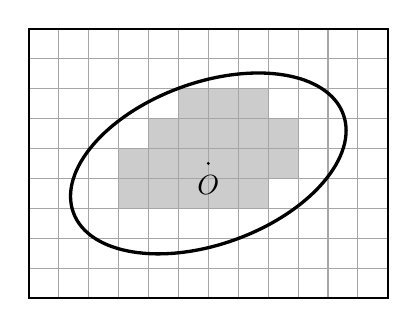
\begin{tikzpicture}[scale=0.38]
  % 填充完全在椭圆内的格子 (Ii \subset Omega)
  \foreach \x/\y in {
    3/3, 4/3, 5/3, 6/3, 7/3,
    3/4, 4/4, 5/4, 6/4, 7/4, 8/4,
    4/5, 5/5, 6/5, 7/5, 8/5,
    5/6, 6/6, 7/6
  } {
    \fill[gray!40] (\x, \y) rectangle (\x+1, \y+1);
  }
  % 网格线
  \draw[step=1, thin, gray!70] (0,0) grid (12,9);
  \draw[thick] (0,0) rectangle (12,9);
  
  % 椭圆
  \draw[very thick] (6, 4.5) ellipse [x radius=4.8, y radius=2.7, rotate=20];
  \fill (6, 4.5) circle (1.5pt) node[below=1pt] {$O$};
\end{tikzpicture}
\end{minipage}\hfill
\begin{minipage}{0.48\linewidth}
\centering
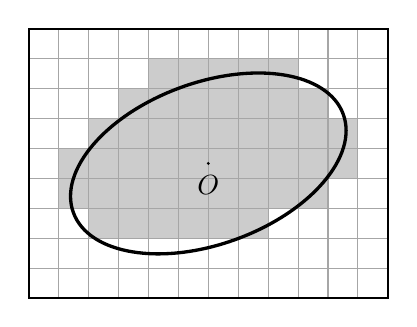
\begin{tikzpicture}[scale=0.38]
  % 填充与椭圆相交的格子 (Omega \cap Ii \neq \emptyset)
  \foreach \x/\y in {
    2/2, 3/2, 4/2, 5/2, 6/2, 7/2,
    1/3, 2/3, 3/3, 4/3, 5/3, 6/3, 7/3, 8/3, 9/3,
    1/4, 2/4, 3/4, 4/4, 5/4, 6/4, 7/4, 8/4, 9/4, 10/4,
    2/5, 3/5, 4/5, 5/5, 6/5, 7/5, 8/5, 9/5, 10/5,
    3/6, 4/6, 5/6, 6/6, 7/6, 8/6, 9/6,
    4/7, 5/7, 6/7, 7/7, 8/7
  } {
    \fill[gray!40] (\x, \y) rectangle (\x+1, \y+1);
  }
  % 网格线
  \draw[step=1, thin, gray!70] (0,0) grid (12,9);
  \draw[thick] (0,0) rectangle (12,9);
  
  % 椭圆
  \draw[very thick] (6, 4.5) ellipse [x radius=4.8, y radius=2.7, rotate=20];
  \fill (6, 4.5) circle (1.5pt) node[below=1pt] {$O$};
\end{tikzpicture}
\end{minipage}
\caption{}
\label{fig:10.2.2}
\end{figure}

\setcounter{definition}{2}
\begin{definitionp}{有面积集的等价定义}\label{def:10.2.2p}
设 $\Omega \subset \mathbb{R}^2$ 为有界集, 闭区间 $I \supset \Omega$, 对 $I$ 的分割 $T = \{I_1, I_2, \cdots, I_k\}$, 有
\[
\bigcup_{I_i\subset\Omega}I_i \subset \Omega \subset \bigcup_{\Omega\cap I_i\neq\varnothing}I_i.
\]
如果
\[
\lim_{\|T\|\to 0}\sum_{\Omega\cap I_i\neq\varnothing}v(I_i) = \lim_{\|T\|\to 0}\sum_{I_i\subset\Omega}v(I_i),
\]
则称 $\Omega$ 为有面积集, 并称 $\lim_{\|T\|\to 0}\sum_{\Omega\cap I_i\neq\varnothing}v(I_i) = \lim_{\|T\|\to 0}\sum_{I_i\subset\Omega}v(I_i)$ 为 $\Omega$ 的面积, 记为 $v(\Omega)$.
\end{definitionp}

\begin{theorem}[有面积集的几何特征二]\label{thm:10.2.5}
设 $\Omega \subset \mathbb{R}^2$ 为有界集. 则 $($图 \ref{fig:10.2.2}$)$
\[
\Omega \text{ 为有面积集} \iff \partial\Omega \text{ 为零面积集, 即 } v(\partial\Omega)=0.
\]
\end{theorem}

\begin{proof}
($\Leftarrow$) 设 $\partial\Omega$ 为零面积集, 即 $v(\partial\Omega)=0$. 又因 1 在 $\Omega$ 上连续, 故 $D_{\text{不}}^1 = \varnothing$, 当然是零面积集. 根据定理 \ref{thm:10.1.4} 知, $\partial\Omega$ 与 $D_{\text{不}}^1$ 都为零测集, 再由定理 \ref{thm:10.2.1} 推得函数 1 在 $\Omega$ 上可积, 即 $\Omega$ 为有面积集.

($\Rightarrow$) 设 $\Omega$ 为有面积集. 任取闭区间 $I \supset \Omega$, 由定理 \ref{thm:10.2.4}, $\forall\varepsilon>0$, $\exists\delta>0$, 当 $\|T\|<\delta$ 时, 有
\[
\sum_{\substack{\Omega\cap I_i\neq\varnothing \\ I_i\not\subset\Omega}}v(I_i) = \sum_{\Omega\cap I_i\neq\varnothing}v(I_i) - \sum_{I_i\subset\Omega}v(I_i) < \frac{\varepsilon}{2}.
\]
固定分割 $T=\{I_1,I_2,\cdots,I_k\}$, 显然 $\bigcup_{i=1}^{k}\partial I_i$ 为零面积集, 从而存在闭区间 $J_1,J_2,\cdots,J_s$, 使得
\[
\bigcup_{i=1}^{k}\partial I_i \subset \bigcup_{j=1}^{s}J_j, \quad \text{且} \quad \sum_{j=1}^{s}v(J_j) < \frac{\varepsilon}{2}.
\]
于是
\[
\partial\Omega \subset \left(\bigcup_{\substack{\Omega\cap I_i\neq\varnothing \\ I_i\not\subset\Omega}}I_i\right) \cup \left(\bigcup_{i=1}^{k}\partial I_i\right) \subset \left(\bigcup_{\substack{\Omega\cap I_i\neq\varnothing \\ I_i\not\subset\Omega}}I_i\right) \cup \left(\bigcup_{j=1}^{s}J_j\right),
\]
且
\[
\sum_{\substack{\Omega\cap I_i\neq\varnothing \\ I_i\not\subset\Omega}}v(I_i) + \sum_{j=1}^{s}v(J_j) < \frac{\varepsilon}{2} + \frac{\varepsilon}{2} = \varepsilon.
\]
这就证明了 $\partial\Omega$ 为零面积集. 再根据定理 \ref{thm:10.2.3}, $v(\partial\Omega)=\int_{\partial\Omega}1=0$.
\end{proof}

\begin{example}\label{ex:10.2.2}
由定理 \ref{thm:10.1.4} 中反例知, $\mathbb{Q}^2 \cap [0,1]^2$ 为 $\mathbb{R}^2$ 中的有界非零面积集. 再由 $v(\partial(\mathbb{Q}^2 \cap [0,1]^2)) = v([0,1]^2) = 1 \neq 0$ 及定理 \ref{thm:10.2.5} 推得 $\mathbb{Q}^2 \cap [0,1]^2$ 不为有面积集. 根据定义 \ref{def:10.2.2}, 1 在 $\Omega$ 上不可积.
\end{example}

\setcounter{definition}{2}
\begin{definitionpp}{有面积集的等价定义}\label{def:10.2.2pp}
设 $\Omega \subset \mathbb{R}^2$ 为有界集. 如果 $\partial\Omega$ 为零面积集, 则称 $\Omega$ 为有面积集.
\end{definitionpp}

因为有时对 $\partial\Omega$ 是否为零面积集的判断比较容易, 所以用这种方法判断 $\Omega$ 是否为有面积集也比较容易. 但是, 这定义不能给出 $\Omega$ 的面积的大小.

\begin{theorem}[有面积集上函数可积的充要条件]\label{thm:10.2.6}
设 $\Omega \subset \mathbb{R}^2$ 为有面积集, $f\colon \Omega \to \mathbb{R}$ 为有界二元函数. 则
\begin{align*}
f \text{ 在 } \Omega \text{ 上可积} &\iff D_{\text{不}}^f = \{(x, y) \in \Omega \mid f \text{ 在 } (x, y) \text{ 处不连续}\} \text{ 为零测集}, \\
&\quad\text{即 } f \text{ 在 } \Omega \text{ 上几乎处处连续}.
\end{align*}
\end{theorem}

\begin{proof}
因为 $\Omega$ 为有面积集, 根据定理 \ref{thm:10.2.5} 知, $\partial\Omega$ 与 $\partial\Omega\cap\Omega$ 都为零面积集, 当然它们也为零测集.

设闭区间 $I \supset \Omega$, 则 $\Omega = \Omega^\circ \cup (\partial \Omega \cap \Omega)$, 且
\[
I = \Omega^\circ \cup \partial\Omega \cup (I\setminus\Omega)^\circ \cup \partial I.
\]
显然, $\partial I$ 为零面积集, 自然也为零测集. 此外, 易见,
\begin{gather*}
f \text{ 在 } \boldsymbol{x} \in \Omega \text{ 不连续} \implies f_{\Omega} \text{ 在 } \boldsymbol{x} \in \Omega \text{ 不连续}; \\
f \text{ 在 } \boldsymbol{x} \in \Omega^\circ \text{ 不连续} \iff f_{\Omega} \text{ 在 } \boldsymbol{x} \in \Omega^\circ \text{ 不连续};
\end{gather*}
$f_{\Omega}$ 在 $(I\setminus\Omega)^\circ$ 上恒为 0, 故它连续.
于是
\[
\begin{cases}
D_{\text{不}}^f \subset D_{\text{不}}^{f_{\Omega}}, \\
D_{\text{不}}^{f_{\Omega}} \subset D_{\text{不}}^f \cup \partial\Omega \cup \partial I.
\end{cases}
\]
这就可推出
\begin{align*}
f \text{ 在 } \Omega \text{ 上可积} &\iff f_{\Omega} \text{ 在 } I \text{ 上可积} \iff D_{\text{不}}^{f_{\Omega}} \text{ 为零测集} \\
&\iff D_{\text{不}}^f \text{ 为零测集, 即 } f \text{ 在 } \Omega \text{ 上几乎处处连续}. \qedhere
\end{align*}
\end{proof}

注意, 0 在任何有界集 $\Omega \subset \mathbb{R}^2$ 上都可积, 不必要求 $\Omega$ 为有面积集. 而定理 \ref{thm:10.2.6} 是在 $\Omega$ 为有面积集的前提下 $f$ 可积的充要条件. 定义 \ref{def:10.2.2} 表明 1 在 $\Omega$ 上可积就是 $\Omega$ 为有面积集.

\begin{example}\label{ex:10.2.3}
设 $\Omega$ 为有限段显式表示的连续曲线围成的区域 (图 \ref{fig:10.2.3}), 根据例 \ref{ex:10.1.1} 知 $\partial\Omega$ 为零面积集, 即 $v(\partial\Omega)=0$. 再根据定理 \ref{thm:10.2.5}, $\Omega$ 为有面积集.

同理, 若 $\Omega$ 为有限段 $C^1$ 参数曲线围成的区域 (图 \ref{fig:10.2.4}), 根据例 \ref{ex:10.1.2} 知, $\partial\Omega$ 为零面积集. 再由定理 \ref{thm:10.2.5}, $\Omega$ 为有面积集.
\end{example}

\begin{figure}[htbp]
\centering
\begin{minipage}{0.48\linewidth}
\centering
\begin{tikzpicture}[scale=0.9, >=Stealth]
  % 坐标轴
  \draw[->] (-0.3, 0) -- (4.2, 0) node[below] {$x$};
  \draw[->] (0, -0.3) -- (0, 3.6) node[left] {$y$};
  \node[below left] at (0,0) {$O$};
  
  % 区域四条曲线:
  \begin{scope}
    \path[clip] (0.5, 0.9) to[bend right=10] (1.1, 0.5)
                           to[bend right=12] (3.0, 0.9)
                           to[bend left=10] (2.3, 2.3)
                           to[bend left=15] (0.5, 0.9);
    \fill[pattern=north east lines, pattern color=black!70] (0,0) rectangle (4,4);
  \end{scope}
  \draw[thick] (0.5, 0.9) to[bend right=10] (1.1, 0.5)
                          to[bend right=12] (3.0, 0.9)
                          to[bend left=10] (2.3, 2.3)
                          to[bend left=15] (0.5, 0.9);
  \node at (1.8, 1.3) {$\Omega$};
  
  % 曲线标注
  \node[left, rotate=38] at (0.7, 0.6) {\scriptsize $x=g_1(y)$};
  \node[below] at (2.0, 0.65) {\scriptsize $y=f_1(x)$};
  \node[right, rotate=-55] at (2.7, 1.7) {\scriptsize $x=g_2(y)$};
  \node[above, rotate=38] at (1.3, 1.8) {\scriptsize $y=f_2(x)$};
\end{tikzpicture}
\caption{}
\label{fig:10.2.3}
\end{minipage}\hfill
\begin{minipage}{0.48\linewidth}
\centering
\begin{tikzpicture}[scale=0.9, >=Stealth]
  % 坐标轴
  \draw[->] (-0.3, 0) -- (4.2, 0) node[below] {$x$};
  \draw[->] (0, -0.3) -- (0, 3.6) node[left] {$y$};
  \node[below left] at (0,0) {$O$};
  
  % 梅花状参数曲线
  \begin{scope}
    \path[clip] (2.0, 0.5) to[out=20, in=200] (2.8, 0.6)
                           to[out=60, in=-40] (2.6, 1.4)
                           to[out=0, in=-90] (3.3, 2.0)
                           to[out=90, in=0] (2.5, 2.6)
                           to[out=140, in=40] (1.5, 2.6)
                           to[out=180, in=90] (0.7, 2.0)
                           to[out=-90, in=180] (1.4, 1.4)
                           to[out=-140, in=120] (1.2, 0.6)
                           to[out=-20, in=160] (2.0, 0.5);
    \fill[pattern=north east lines, pattern color=black!70] (0,0) rectangle (4,4);
  \end{scope}
  \draw[thick] (2.0, 0.5) to[out=20, in=200] (2.8, 0.6)
                          to[out=60, in=-40] (2.6, 1.4)
                          to[out=0, in=-90] (3.3, 2.0)
                          to[out=90, in=0] (2.5, 2.6)
                          to[out=140, in=40] (1.5, 2.6)
                          to[out=180, in=90] (0.7, 2.0)
                          to[out=-90, in=180] (1.4, 1.4)
                          to[out=-140, in=120] (1.2, 0.6)
                          to[out=-20, in=160] (2.0, 0.5);
  \node at (2.0, 1.7) {$\Omega$};
  \node[right] at (3.3, 2.0) {\small $(x(t), y(t))$};
\end{tikzpicture}
\caption{}
\label{fig:10.2.4}
\end{minipage}
\end{figure}

上面所述的区域 $\Omega$ 是数学分析中常见的集合. 再从定理 \ref{thm:10.2.6} 立即得到
\[
f\colon\Omega\to\mathbb{R} \text{ 可积} \iff f \text{ 在 } \Omega \text{ 上几乎处处连续}.
\]

最后, 我们来讨论可积函数的一些性质.

\begin{theorem}\label{thm:10.2.7}
设 $\Omega \subset \mathbb{R}^2$ 为有界集, $f, f_1, f_2\colon \Omega \to \mathbb{R}$ 都为二元函数, $c \in \mathbb{R}$ 为常数.
\begin{enumerate}
\item 如果 $\Omega$ 为有面积集, 则 $c$ 在 $\Omega$ 上可积, 且
\[
\int_{\Omega}c = c v(\Omega).
\]
\item 如果 $f$ 在 $\Omega$ 上可积, 则 $cf$ 在 $\Omega$ 上也可积, 且
\[
\int_{\Omega}cf = c\int_{\Omega}f.
\]
\item 如果 $f_{1}$ 与 $f_{2}$ 都在 $\Omega$ 上可积, 则 $f_{1} + f_{2}$ 在 $\Omega$ 上也可积, 且
\[
\int_{\Omega}(f_{1}+f_{2}) = \int_{\Omega}f_{1} + \int_{\Omega}f_{2}.
\]
\item 如果 $f$ 在 $\Omega$ 上可积, 且 $f \geqslant 0$, 则
\[
\int_{\Omega}f \geqslant 0;
\]
特别地, 若 $f_{1}$ 与 $f_{2}$ 都在 $\Omega$ 上可积, 且 $f_{1} \geqslant f_{2}$, 则
\[
\int_{\Omega}f_{1} \geqslant \int_{\Omega}f_{2}.
\]
\item 如果 $f$ 在 $\Omega$ 上可积, 则 $|f|$ 在 $\Omega$ 上也可积, 且
\[
\left|\int_{\Omega}f\right| \leqslant \int_{\Omega}|f|.
\]
\end{enumerate}
\end{theorem}

\begin{proof}
设 $I \subset \mathbb{R}^2$ 为闭区间, 且 $I \supset \Omega$. 先证 (2), 再证 (1).

(2) $\int_{\Omega} cf = \int_{I}(cf)_{\Omega} = \int_{I} cf_{\Omega} = c\int_{I} f_{\Omega} = c\int_{\Omega} f$.

(1) 因为 $\Omega$ 为有面积集, 由 (2) 知 $c = c \cdot 1$ 在 $\Omega$ 上也可积, 且
\[
\int_{\Omega}c = \int_{\Omega}c \cdot 1 = c\int_{\Omega}1 = c v(\Omega).
\]

(3) 因为 $f_{1}$ 与 $f_{2}$ 都在 $\Omega$ 上可积, 故 $f_{1\Omega}$ 与 $f_{2\Omega}$ 都在 $I$ 上可积, 从而 $(f_{1}+f_{2})_{\Omega}=f_{1\Omega}+f_{2\Omega}$ 也在 $I$ 上可积, 即 $f_{1}+f_{2}$ 在 $\Omega$ 上可积, 且
\[
\int_{\Omega}(f_{1}+f_{2}) = \int_{I}(f_{1}+f_{2})_{\Omega} = \int_{I}(f_{1\Omega}+f_{2\Omega}) = \int_{I}f_{1\Omega} + \int_{I}f_{2\Omega} = \int_{\Omega}f_{1} + \int_{\Omega}f_{2}.
\]

(4) 因为在 $\Omega$ 上 $f \geqslant 0$, 所以 $f_{\Omega} \geqslant 0$. 根据定理 \ref{thm:10.1.1}(4), 有
\[
\int_{\Omega}f = \int_{I}f_{\Omega} \geqslant 0.
\]
从而
\[
\int_{\Omega}f_{1} - \int_{\Omega}f_{2} = \int_{\Omega}(f_{1}-f_{2}) \geqslant 0,
\]
\[
\int_{\Omega}f_{1} \geqslant \int_{\Omega}f_{2}.
\]

(5) 因为 $f$ 在 $\Omega$ 上可积, 所以 $f_{\Omega}$ 在 $I$ 上可积, 从而 $|f|_{\Omega}=|f_{\Omega}|$ 在 $I$ 上可积. 再由
\[
-|f| \leqslant f \leqslant |f|
\]
及 (4) 得到
\begin{gather*}
-\int_{\Omega}|f| \leqslant \int_{\Omega}f \leqslant \int_{\Omega}|f|, \\
\left|\int_{\Omega}f\right| \leqslant \int_{\Omega}|f|. \qedhere
\end{gather*}
\end{proof}

\begin{theorem}[积分的集合可加性]\label{thm:10.2.8}
设 $\Omega_{1}, \Omega_{2} \subset \mathbb{R}^{2}$ 都为有界集, 且 $\Omega_{1} \cap \Omega_{2}$ 为一零面积集 $(\Omega_{1} \cap \Omega_2 = \varnothing$ 为其特例$)$. 若函数 $f$ 在 $\Omega_{1}$ 与 $\Omega_{2}$ 上都可积, 则 $f$ 在 $\Omega_{1} \cup \Omega_{2}$ 上也可积, 且
\[
\int_{\Omega_{1}\cup\Omega_{2}}f = \int_{\Omega_{1}}f + \int_{\Omega_{2}}f.
\]
\end{theorem}

\begin{proof}
显然, 除了一个零面积集, 成立等式 $f_{\Omega_1 \cup \Omega_2} = f_{\Omega_1} + f_{\Omega_2}$. 设闭区间 $I \supset \Omega_1 \cup \Omega_2$, 则有
\[
\int_{\Omega_{1}}f + \int_{\Omega_{2}}f = \int_{I}f_{\Omega_{1}} + \int_{I}f_{\Omega_{2}} = \int_{I}(f_{\Omega_{1}}+f_{\Omega_{2}}) \reason{\text{例 \ref{ex:10.1.5}}} \int_{I}f_{\Omega_{1}\cup\Omega_{2}} = \int_{\Omega_{1}\cup\Omega_{2}}f. \qedhere
\]
\end{proof}

\begin{theorem}[积分中值定理]\label{thm:10.2.9}
设 $\Omega \subset \mathbb{R}^2$ 为有面积的连通紧致集, $f, g\colon \Omega \to \mathbb{R}$ 连续, 且 $g$ 在 $\Omega$ 上不变号, 则 $\exists\boldsymbol{\xi} \in \Omega$, s.t.
\[
\int_{\Omega}f g = f(\boldsymbol{\xi})\int_{\Omega}g.
\]
特别地, 取 $g=1$, 则 $\exists\boldsymbol{\xi} \in \Omega$, s.t.
\[
\int_{\Omega}f = f(\boldsymbol{\xi})v(\Omega).
\]
\end{theorem}

\begin{proof}
因为 $\Omega$ 为有面积集, 根据定理 \ref{thm:10.2.5}, $v(\partial\Omega)=0$ (即 $\partial\Omega$ 为零面积集). 由于 $f, g$ 在 $\Omega$ 上连续, 故 $fg$ 在 $\Omega$ 上也连续. 再根据定理 \ref{thm:10.2.1} 或定理 \ref{thm:10.2.6}, $g$ 与 $fg$ 都在 $\Omega$ 上可积. 又因 $\Omega$ 紧致, 故连续函数 $f$ 在 $\Omega$ 上达到最大值与最小值, 所以 $\exists\boldsymbol{p}, \boldsymbol{q} \in \Omega$, s.t.
\[
f(\boldsymbol{p}) = \max f(\Omega), \quad f(\boldsymbol{q}) = \min f(\Omega).
\]
从题设 $g$ 在 $\Omega$ 上不变号, 不妨设 $g|_{\Omega} \geqslant 0$. 于是
\[
f(\boldsymbol{q})g \leqslant fg \leqslant f(\boldsymbol{p})g.
\]
根据定理 \ref{thm:10.2.7}(4), (2), 有
\[
f(\boldsymbol{q})\int_{\Omega}g \leqslant \int_{\Omega}fg \leqslant f(\boldsymbol{p})\int_{\Omega}g.
\]
(1) 若 $\int_{\Omega}g=0$, 由 $g$ 非负连续, $g|_{\Omega}\equiv 0$, 则 $\int_{\Omega}fg=0=f(\boldsymbol{\xi})\cdot 0=f(\boldsymbol{\xi})\int_{\Omega}g$, $\forall\boldsymbol{\xi}\in\Omega$.

(2) 若 $\int_{\Omega}g\neq 0$, 由 $g\geqslant 0$ 知 $\int_{\Omega}g>0$. 于是
\[
f(\boldsymbol{q}) \leqslant \frac{\displaystyle\int_{\Omega}fg}{\displaystyle\int_{\Omega}g} \leqslant f(\boldsymbol{p}).
\]
再由 $\Omega$ 连通, 应用连续函数的介值定理, $\exists\boldsymbol{\xi}\in\Omega$, s.t.
\[
\frac{\displaystyle\int_{\Omega}fg}{\displaystyle\int_{\Omega}g} = f(\boldsymbol{\xi}),
\]
即
\[
\int_{\Omega}fg = f(\boldsymbol{\xi})\int_{\Omega}g. \qedhere
\]
\end{proof}

\begin{exblock}{练习题 10.2}
1. 设 $f$ 为连续函数, 求极限
\[
\lim_{r \to 0}\frac{1}{\pi r^2}\iint_{x^2 + y^2 \leqslant r^2} f(x, y)\,\mathrm{d}x\mathrm{d}y.
\]

2. 证明:
\[
1.96 < \iint_{|x|+|y|\leqslant 10}\frac{\mathrm{d}x\mathrm{d}y}{100 + \cos^2 x + \cos^2 y} < 2.
\]
\end{exblock}

\section{化二重积分为累次积分}\label{sec:10.3}

在第 \ref{sec:10.1} 节中，我们建立了二重积分的定义，并且证明了二重积分具有类似于定积分的许多性质。
但是，直接由定义计算二重积分，即使对比较简单的函数与区域来说，也是很困难的。
为了求出二重积分的值，必须寻找更方便的计算方法。
在微积分学中，计算重积分的基本方法是：把重积分化为一连串的一元函数的定积分（通常称为累次积分或多次积分）来计算。
本节我们来讨论如何把二重积分化为两次定积分来计算。

首先，我们讨论在闭矩形区间上的情形。

\begin{theorem}\label{thm:10.3.1}
设 $I = [a, b] \times [c, d]$ 为 $\mathbb{R}^2$ 中的闭区间，$f\colon I \to \mathbb{R}$ 可积，则单变量函数
\[
I_1(x) = \overline{\int_c^d} f(x, y)\,\mathrm{d}y, \quad I_2(x) = \underline{\int_c^d} f(x, y)\,\mathrm{d}y
\]
在 $[a, b]$ 上都可积，且
\[
\int_a^b \overline{\int_c^d} f(x, y)\,\mathrm{d}y\,\mathrm{d}x = \int_a^b \underline{\int_c^d} f(x, y)\,\mathrm{d}y\,\mathrm{d}x = \iint_I f(x, y)\,\mathrm{d}x\mathrm{d}y.
\]
\end{theorem}

\begin{proof}
设 $T_1 = \{a = x_0 < x_1 < \cdots < x_m = b\}$ 与 $T_2 = \{c = y_0 < y_1 < \cdots < y_k = d\}$ 分别为 $[a, b]$ 与 $[c, d]$ 的任意分割。
它们构成了闭区间 $I$ 的一个网格分割 $T = T_1 \times T_2$。
记
\[
I_{ij} = [x_{i-1}, x_i] \times [y_{j-1}, y_j], \quad v(I_{ij}) = \Delta x_i \Delta y_j = (x_i - x_{i-1})(y_j - y_{j-1}),
\]
\[
m_{ij} = \inf_{(x, y) \in I_{ij}} f(x, y), \quad M_{ij} = \sup_{(x, y) \in I_{ij}} f(x, y).
\]
对于固定的 $x \in [x_{i-1}, x_i]$，记
\[
m_j(x) = \inf_{y \in [y_{j-1}, y_j]} f(x, y), \quad M_j(x) = \sup_{y \in [y_{j-1}, y_j]} f(x, y).
\]
显然对任意 $y \in [y_{j-1}, y_j]$，恒有 $m_{ij} \leqslant m_j(x) \leqslant f(x, y) \leqslant M_j(x) \leqslant M_{ij}$。
从而根据上、下积分的定义与性质，有
\[
\sum_{j=1}^k m_{ij} \Delta y_j \leqslant \sum_{j=1}^k m_j(x) \Delta y_j \leqslant \underline{\int_c^d} f(x, y)\,\mathrm{d}y \leqslant \overline{\int_c^d} f(x, y)\,\mathrm{d}y \leqslant \sum_{j=1}^k M_j(x) \Delta y_j \leqslant \sum_{j=1}^k M_{ij} \Delta y_j.
\]
上式对任意 $x \in [x_{i-1}, x_i]$ 均成立。
故在区间 $[x_{i-1}, x_i]$ 上分别取 $I_1(x) = \overline{\int_c^d} f(x, y)\,\mathrm{d}y$ 与 $I_2(x) = \underline{\int_c^d} f(x, y)\,\mathrm{d}y$ 的下确界与上确界，即知
\[
\sum_{j=1}^k m_{ij} \Delta y_j \leqslant \inf_{x \in [x_{i-1}, x_i]} I_2(x) \leqslant \sup_{x \in [x_{i-1}, x_i]} I_1(x) \leqslant \sum_{j=1}^k M_{ij} \Delta y_j.
\]
两边同乘以 $\Delta x_i$，并对 $i = 1, 2, \dots, m$ 求和，得
\[
s(T, f) = \sum_{i=1}^m \sum_{j=1}^k m_{ij} \Delta x_i \Delta y_j \leqslant s(T_1, I_2) \leqslant s(T_1, I_1) \leqslant S(T_1, I_1) \leqslant S(T, f).
\]
同理亦有
\[
s(T, f) \leqslant s(T_1, I_2) \leqslant S(T_1, I_2) \leqslant S(T_1, I_1) \leqslant S(T, f).
\]
因 $f$ 在 $I$ 上可积，故当 $\|T\| \to 0$ 时，Darboux 和极限存在且
\[
\lim_{\|T\| \to 0} s(T, f) = \lim_{\|T\| \to 0} S(T, f) = \iint_I f(x, y)\,\mathrm{d}x\mathrm{d}y.
\]
注意 $\|T_1\| \leqslant \|T\|$，由夹逼准则立即推得：$I_1(x)$ 与 $I_2(x)$ 在 $[a, b]$ 上均满足 Riemann 可积准则，从而在 $[a, b]$ 上可积，且极限值恰为 $\iint_I f(x, y)\,\mathrm{d}x\mathrm{d}y$。
\end{proof}

由定理 \ref{thm:10.3.1} 立即得到下面两个重要推论：

\begin{theorem}[闭区间上化二重积分为累次积分]\label{thm:10.3.2}
设 $f$ 在闭区间 $I = [a, b] \times [c, d]$ 上可积。如果对每个固定的 $x \in [a, b]$，函数 $f(x, \cdot)$ 在 $[c, d]$ 上都可积，则
\[
\iint_I f(x, y)\,\mathrm{d}x\mathrm{d}y = \int_a^b \mathrm{d}x \int_c^d f(x, y)\,\mathrm{d}y = \int_a^b \left( \int_c^d f(x, y)\,\mathrm{d}y \right) \mathrm{d}x.
\]
\end{theorem}

\begin{proof}
因 $f(x, \cdot)$ 在 $[c, d]$ 上可积，故对每个 $x \in [a, b]$，其上积分与下积分相等：
\[
\overline{\int_c^d} f(x, y)\,\mathrm{d}y = \underline{\int_c^d} f(x, y)\,\mathrm{d}y = \int_c^d f(x, y)\,\mathrm{d}y.
\]
代入定理 \ref{thm:10.3.1} 即得所证。
\end{proof}

同理，若先对 $x$ 积分再对 $y$ 积分，亦有完全对称的结论：

\begin{theorem}[闭区间上化二重积分为累次积分]\label{thm:10.3.3}
设 $f$ 在 $I = [a, b] \times [c, d]$ 上可积，且对每个 $x \in [a, b]$，$f(x, \cdot)$ 在 $[c, d]$ 上可积；又对每个 $y \in [c, d]$，$f(\cdot, y)$ 在 $[a, b]$ 上可积，则
\[
\iint_I f(x, y)\,\mathrm{d}x\mathrm{d}y = \int_a^b \mathrm{d}x \int_c^d f(x, y)\,\mathrm{d}y = \int_c^d \mathrm{d}y \int_a^b f(x, y)\,\mathrm{d}x.
\]
特别地，当 $f$ 在 $I$ 上连续时，上述可积性条件自然满足，累次积分顺序可以任意交换。
\end{theorem}

现在，我们把闭矩形区间上的结论推广到一般的有界有面积集 $\Omega \subset \mathbb{R}^2$ 上。

\begin{figure}[htbp]
\centering
\begin{tikzpicture}[>=Stealth, scale=1.0]
  \draw[->] (-0.3,0) -- (5.2,0) node[below] {$x$};
  \draw[->] (0,-0.3) -- (0,4.2) node[left] {$y$};
  \node[below left] at (0,0) {$O$};

  \coordinate (A) at (1.0,0);
  \coordinate (X) at (2.2,0);
  \coordinate (B) at (4.4,0);
  \coordinate (C) at (0,0.8);
  \coordinate (Y) at (0,2.3);
  \coordinate (D) at (0,3.6);

  \node[below] at (A) {$a$};
  \node[below] at (X) {$x$};
  \node[below] at (B) {$b$};
  \node[left] at (C) {$c$};
  \node[left] at (Y) {$y$};
  \node[left] at (D) {$d$};

  \draw[dashed] (1.0,0) -- (1.0,3.8);
  \draw[dashed] (4.4,0) -- (4.4,3.8);
  \draw[dashed] (0,0.8) -- (4.8,0.8);
  \draw[dashed] (0,3.6) -- (4.8,3.6);

  \draw[dashed] (2.2,0) -- (2.2,1.35);
  \draw[dashed] (2.2,2.95) -- (2.2,3.8);
  \draw[dashed] (0,2.3) -- (1.35,2.3);
  \draw[dashed] (3.65,2.3) -- (4.8,2.3);

  \draw[thick, fill=black!15] 
    (1.3, 2.0) .. controls (1.5, 2.9) and (2.5, 3.1) .. (3.2, 2.8)
    .. controls (3.6, 2.6) and (3.8, 2.3) .. (4.2, 2.7)
    -- (4.2, 1.4)
    .. controls (3.8, 1.8) and (3.6, 1.5) .. (3.2, 1.3)
    .. controls (2.5, 1.0) and (1.5, 1.2) .. (1.3, 2.0) -- cycle;

  \draw[very thick] (2.2, 1.15) -- (2.2, 2.97);
  \node[right] at (2.2, 1.7) {$\Omega_x$};

  \draw[very thick] (1.33, 2.3) -- (3.68, 2.3);
  \node[above] at (1.8, 2.3) {$\Omega^y$};

  \node at (2.9, 2.0) {$\Omega$};

  \draw[decorate, decoration={brace, mirror, amplitude=5pt}] (1.0, -0.3) -- (4.4, -0.3) node[midway, below=5pt] {$I$};
  \draw[decorate, decoration={brace, amplitude=5pt}] (-0.3, 0.8) -- (-0.3, 3.6) node[midway, left=5pt] {$J$};
\end{tikzpicture}
\caption{}\label{fig:10.3.1}
\end{figure}

\begin{theorem}[有界集上化二重积分为累次积分]\label{thm:10.3.4}
设 $\Omega \subset \mathbb{R}^2$ 为有面积集，$f\colon \Omega \to \mathbb{R}$ 有界且连续。记 $\Omega$ 在 $x$ 轴上的垂直投影（图 \ref{fig:10.3.1}）为
\[
I = \{x \in \mathbb{R} \mid \exists y, \text{ s.t. } (x, y) \in \Omega\}.
\]
如果对每个 $x \in I$，截线集 $\Omega_x = \{y \in \mathbb{R} \mid (x, y) \in \Omega\}$ 为一个或有限个区间的并（可以退缩为单点），则
\[
\iint_\Omega f = \int_I \mathrm{d}x \int_{\Omega_x} f(x, y)\,\mathrm{d}y.
\]
同样，记 $\Omega$ 在 $y$ 轴上的垂直投影（图 \ref{fig:10.3.1}）为
\[
J = \{y \in \mathbb{R} \mid \exists x, \text{ s.t. } (x, y) \in \Omega\}.
\]
如果对每个 $y \in J$，截线集 $\Omega^y = \{x \in \mathbb{R} \mid (x, y) \in \Omega\}$ 为一个或有限个区间的并（可以退缩为单点），则
\[
\iint_\Omega f = \int_J \mathrm{d}y \int_{\Omega^y} f(x, y)\,\mathrm{d}x.
\]
\end{theorem}

\begin{proof}
作闭区间 $[a, b] \times [c, d] \supset \Omega$（图 \ref{fig:10.3.1}）。
因为 $f$ 在 $\Omega$ 上有界连续，并且 $\Omega \subset \mathbb{R}^2$ 为有面积集，根据定理 \ref{thm:10.2.6}，$f$ 在 $\Omega$ 上可积。
再由定义 \ref{def:10.2.1}，零延拓函数 $f_\Omega$ 在 $[a, b] \times [c, d]$ 上可积，且
\[
\iint_\Omega f = \iint_{[a, b] \times [c, d]} f_\Omega.
\]
当 $x \in I$ 时，函数 $f(x, \cdot)$ 在区间 $\Omega_x$ 上有界且连续，所以 $f(x, \cdot)$ 在 $\Omega_x$ 上可积。
又因在 $[c, d] \setminus \Omega_x$ 上 $f_\Omega(x, y) = 0$，故 $f_\Omega(x, \cdot)$ 在 $[c, d]$ 上可积，且
\[
\int_c^d f_\Omega(x, y)\,\mathrm{d}y = \int_{\Omega_x} f(x, y)\,\mathrm{d}y.
\]
当 $x \in [a, b] \setminus I$ 时，对一切 $y \in [c, d]$ 均有 $f_\Omega(x, y) = 0$，从而
\[
\int_c^d f_\Omega(x, y)\,\mathrm{d}y = 0.
\]
根据定理 \ref{thm:10.3.2}，有
\begin{align*}
\iint_\Omega f &= \iint_{[a, b] \times [c, d]} f_\Omega = \int_a^b \mathrm{d}x \int_c^d f_\Omega(x, y)\,\mathrm{d}y \\
&= \int_I \mathrm{d}x \int_c^d f_\Omega(x, y)\,\mathrm{d}y = \int_I \mathrm{d}x \int_{\Omega_x} f(x, y)\,\mathrm{d}y.
\end{align*}
对称地可证第二式。
\end{proof}

考虑应用中最常见的两类特殊区域（通常称为 $X$-型区域与 $Y$-型区域）：

\begin{figure}[htbp]
\centering
\begin{minipage}[b]{0.48\linewidth}
\centering
\begin{tikzpicture}[>=Stealth, scale=0.95]
  \draw[->] (-0.3,0) -- (4.2,0) node[below] {$x$};
  \draw[->] (0,-0.3) -- (0,3.8) node[left] {$y$};
  \node[below left] at (0,0) {$O$};

  \coordinate (A) at (0.9,0);
  \coordinate (X) at (1.9,0);
  \coordinate (B) at (3.5,0);
  \node[below] at (A) {$a$};
  \node[below] at (X) {$x$};
  \node[below] at (B) {$b$};

  \draw[dashed] (0, 0.8) node[left] {$c$} -- (3.8, 0.8);
  \draw[dashed] (0, 3.2) node[left] {$d$} -- (3.8, 3.2);

  \draw[dashed] (0.9, 0) -- (0.9, 1.0);
  \draw[dashed] (3.5, 0) -- (3.5, 1.1);

  \draw[thick, fill=black!15]
    (0.9, 1.0) .. controls (1.8, 1.6) and (2.6, 0.8) .. (3.5, 1.1)
    -- (3.5, 2.9)
    .. controls (2.6, 3.2) and (1.8, 2.6) .. (0.9, 2.7)
    -- cycle;

  \draw[dashed] (1.9,0) -- (1.9, 1.25);
  \draw[very thick] (1.9, 1.25) -- (1.9, 2.85);
  \node[right] at (1.9, 2.1) {$\Omega_x$};

  \node[below] at (3.0, 1.0) {$y=y_1(x)$};
  \node[above] at (3.0, 2.9) {$y=y_2(x)$};
  \node at (3.1, 2.0) {$\Omega$};
\end{tikzpicture}
\caption{}\label{fig:10.3.2}
\end{minipage}
\hfill
\begin{minipage}[b]{0.48\linewidth}
\centering
\begin{tikzpicture}[>=Stealth, scale=0.95]
  \draw[->] (-0.3,0) -- (4.2,0) node[below] {$x$};
  \draw[->] (0,-0.3) -- (0,3.8) node[left] {$y$};
  \node[below left] at (0,0) {$O$};

  \draw[dashed] (0, 0.9) node[left] {$c$} -- (3.8, 0.9);
  \draw[dashed] (0, 3.2) node[left] {$d$} -- (3.8, 3.2);

  \draw[dashed] (1.5, 0) -- (1.5, 3.5);
  \draw[dashed] (3.5, 0) -- (3.5, 3.5);

  \draw[thick, fill=black!15]
    (1.7, 0.9) .. controls (1.5, 1.8) and (2.2, 2.4) .. (1.8, 3.2)
    -- (3.4, 3.2)
    .. controls (3.8, 2.4) and (3.1, 1.8) .. (3.3, 0.9)
    -- cycle;

  \draw[dashed] (0, 2.1) node[left] {$y$} -- (1.85, 2.1);
  \draw[very thick] (1.85, 2.1) -- (3.3, 2.1);
  \node[above] at (2.6, 2.1) {$\Omega^y$};

  \node[left] at (1.7, 1.4) {$x=x_1(y)$};
  \node[right] at (3.3, 1.4) {$x=x_2(y)$};
  \node at (2.7, 1.3) {$\Omega$};
\end{tikzpicture}
\caption{}\label{fig:10.3.3}
\end{minipage}
\end{figure}

\begin{theorem}[有界集上化二重积分为累次积分]\label{thm:10.3.5}
设
\[
\Omega = \{(x, y) \in \mathbb{R}^2 \mid y_1(x) \leqslant y \leqslant y_2(x), a \leqslant x \leqslant b\},
\]
其中函数 $y_1$ 与 $y_2$ 在 $[a, b]$ 上连续（图 \ref{fig:10.3.2}），函数 $f$ 在 $\Omega$ 上可积。
如果对每个 $x \in [a, b]$，单变量积分 $\int_{y_1(x)}^{y_2(x)} f(x, y)\,\mathrm{d}y$ 存在，则
\[
\iint_\Omega f = \int_a^b \mathrm{d}x \int_{y_1(x)}^{y_2(x)} f(x, y)\,\mathrm{d}y.
\]
\end{theorem}

\begin{proof}
取闭区间 $[a, b] \times [c, d] \supset \Omega$。
对于固定的 $x \in [a, b]$，因为 $f(x, \cdot)$ 在 $[y_1(x), y_2(x)]$ 上可积，且在 $[c, y_1(x))$ 与 $(y_2(x), d]$ 上零延拓值恒为 $0$，故 $f_\Omega(x, \cdot)$ 在 $[c, d]$ 上可积，且
\begin{align*}
\int_c^d f_\Omega(x, y)\,\mathrm{d}y &= \int_c^{y_1(x)} f_\Omega(x, y)\,\mathrm{d}y + \int_{y_1(x)}^{y_2(x)} f_\Omega(x, y)\,\mathrm{d}y + \int_{y_2(x)}^d f_\Omega(x, y)\,\mathrm{d}y \\
&= 0 + \int_{y_1(x)}^{y_2(x)} f(x, y)\,\mathrm{d}y + 0 = \int_{y_1(x)}^{y_2(x)} f(x, y)\,\mathrm{d}y.
\end{align*}
根据定理 \ref{thm:10.3.2}，
\[
\iint_\Omega f = \int_a^b \mathrm{d}x \int_c^d f_\Omega(x, y)\,\mathrm{d}y = \int_a^b \mathrm{d}x \int_{y_1(x)}^{y_2(x)} f(x, y)\,\mathrm{d}y. \qedhere
\]
\end{proof}

对称地，对于 $Y$-型区域（图 \ref{fig:10.3.3}），有：

\begin{theorem}[有界集上化二重积分为累次积分]\label{thm:10.3.6}
设
\[
\Omega = \{(x, y) \in \mathbb{R}^2 \mid x_1(y) \leqslant x \leqslant x_2(y), c \leqslant y \leqslant d\},
\]
其中函数 $x_1$ 与 $x_2$ 在 $[c, d]$ 上连续（图 \ref{fig:10.3.3}），函数 $f$ 在 $\Omega$ 上可积。
如果对每个 $y \in [c, d]$，单变量积分 $\int_{x_1(y)}^{x_2(y)} f(x, y)\,\mathrm{d}x$ 存在，则
\[
\iint_\Omega f = \int_c^d \mathrm{d}y \int_{x_1(y)}^{x_2(y)} f(x, y)\,\mathrm{d}x.
\]
\end{theorem}

\begin{proof}
类似定理 \ref{thm:10.3.5} 的证明。
\end{proof}

下面我们通过一系列典型例题，详细介绍化二重积分为累次积分的具体计算方法、技巧与几何应用。

\begin{example}\label{ex:10.3.1}
计算二重积分
\[
\iint_{\substack{0 \leqslant x \leqslant 1 \\ 0 \leqslant y \leqslant 1}} x \mathrm{e}^{xy}\,\mathrm{d}x\mathrm{d}y.
\]
\end{example}

\begin{solution}
积分区域为闭矩形区间 $I = [0, 1] \times [0, 1]$，被积函数连续。
若先对 $x$ 积分，需要用分部积分法；而若先对 $y$ 积分，计算则极为简便：
\begin{align*}
\iint_I x \mathrm{e}^{xy}\,\mathrm{d}x\mathrm{d}y &= \int_0^1 \mathrm{d}x \int_0^1 x \mathrm{e}^{xy}\,\mathrm{d}y = \int_0^1 \left[ \mathrm{e}^{xy} \Big|_{y=0}^{y=1} \right] \mathrm{d}x \\
&= \int_0^1 (\mathrm{e}^x - 1)\,\mathrm{d}x = (\mathrm{e}^x - x)\Big|_0^1 = \mathrm{e} - 2. \qedhere
\end{align*}
\end{solution}

\begin{example}\label{ex:10.3.2}
计算二重积分
\[
\iint_{[0, \pi] \times [0, 1]} y \sin(xy)\,\mathrm{d}x\mathrm{d}y.
\]
\end{example}

\begin{solution}
先对 $x$ 积分再对 $y$ 积分：
\begin{align*}
\iint_{[0, \pi] \times [0, 1]} y \sin(xy)\,\mathrm{d}x\mathrm{d}y &= \int_0^1 \mathrm{d}y \int_0^\pi y \sin(xy)\,\mathrm{d}x = \int_0^1 \left[ -\cos(xy) \Big|_{x=0}^{x=\pi} \right] \mathrm{d}y \\
&= \int_0^1 (1 - \cos(\pi y))\,\mathrm{d}y = \left( y - \frac{\sin(\pi y)}{\pi} \right) \Bigg|_0^1 = 1. \qedhere
\end{align*}
\end{solution}

\begin{example}\label{ex:10.3.3}
计算
\[
\iint_{\substack{0 \leqslant x \leqslant 1 \\ 0 \leqslant y \leqslant 1}} x \mathrm{e}^{x^2+y^2}\,\mathrm{d}x\mathrm{d}y.
\]
\end{example}

\begin{solution}
由于被积函数可以分离变量 $x \mathrm{e}^{x^2+y^2} = (x \mathrm{e}^{x^2})(\mathrm{e}^{y^2})$，且积分区域为矩形，故累次积分可拆为两个独立的单变量定积分之积：
\[
\iint_{\substack{0 \leqslant x \leqslant 1 \\ 0 \leqslant y \leqslant 1}} x \mathrm{e}^{x^2+y^2}\,\mathrm{d}x\mathrm{d}y = \left( \int_0^1 x \mathrm{e}^{x^2}\,\mathrm{d}x \right) \left( \int_0^1 \mathrm{e}^{y^2}\,\mathrm{d}y \right) = \frac{1}{2}(\mathrm{e} - 1) \int_0^1 \mathrm{e}^{y^2}\,\mathrm{d}y.
\]
注意 $\int_0^1 \mathrm{e}^{y^2}\,\mathrm{d}y$ 的原函数不能用初等函数表示，但作为定积分其值是一个确定的常数。
\end{solution}

\begin{example}\label{ex:10.3.4}
计算二重积分
\[
\iint_\Omega x y^3 \mathrm{e}^{x^2+y^2}\,\mathrm{d}x\mathrm{d}y,
\]
其中 $\Omega = [0, 1] \times [0, 1]$。
\end{example}

\begin{solution}
利用乘积可分离性，有
\begin{align*}
\iint_\Omega x y^3 \mathrm{e}^{x^2+y^2}\,\mathrm{d}x\mathrm{d}y &= \left( \int_0^1 x \mathrm{e}^{x^2}\,\mathrm{d}x \right) \left( \int_0^1 y^3 \mathrm{e}^{y^2}\,\mathrm{d}y \right) \\
&= \frac{1}{2}(\mathrm{e} - 1) \cdot \frac{1}{2} \int_0^1 t \mathrm{e}^t\,\mathrm{d}t \quad (\text{令 } t = y^2) \\
&= \frac{1}{4}(\mathrm{e} - 1) \left[ t \mathrm{e}^t \Big|_0^1 - \int_0^1 \mathrm{e}^t\,\mathrm{d}t \right] \\
&= \frac{1}{4}(\mathrm{e} - 1) (\mathrm{e} - (\mathrm{e} - 1)) = \frac{1}{4}(\mathrm{e} - 1). \qedhere
\end{align*}
\end{solution}

\begin{example}\label{ex:10.3.5}
计算二重积分
\[
\iint_{\substack{0 \leqslant x \leqslant 2 \\ 0 \leqslant y \leqslant 2}} [x + y]\,\mathrm{d}x\mathrm{d}y,
\]
其中 $[u]$ 表示不超过 $u$ 的最大整数。
\end{example}

\begin{figure}[htbp]
\centering
\begin{minipage}[b]{0.48\linewidth}
\centering
\begin{tikzpicture}[>=Stealth, scale=1.3]
  \draw[->] (-0.2,0) -- (2.6,0) node[below] {$x$};
  \draw[->] (0,-0.2) -- (0,2.6) node[left] {$y$};
  \node[below left] at (0,0) {$O$};

  \draw[thick] (0,0) rectangle (2,2);
  \node[left] at (0,1) {$1$};
  \node[left] at (0,2) {$2$};
  \node[below] at (1,0) {$1$};
  \node[below] at (2,0) {$2$};

  \draw[thick] (0,1) -- (1,0);
  \draw[thick] (0,2) -- (2,0);
  \draw[thick] (1,2) -- (2,1);

  \draw[dashed] (1,0) -- (1,2);

  \node[above right, font=\footnotesize] at (0.3, 0.6) {$y=1-x$};
  \node[above right, font=\footnotesize] at (0.8, 1.1) {$y=2-x$};
  \node[above right, font=\footnotesize] at (1.3, 1.6) {$y=3-x$};
  \draw[thick] (1.7, 2.3) -- (2.3, 1.7) node[above right, font=\footnotesize] {$y=4-x$};
  \fill (2,2) circle (1.2pt) node[above left, font=\footnotesize] {$(2,2)$};
\end{tikzpicture}
\caption{}\label{fig:10.3.4}
\end{minipage}
\hfill
\begin{minipage}[b]{0.48\linewidth}
\centering
\begin{tikzpicture}[>=Stealth, scale=1.3]
  \draw[->] (-0.2,0) -- (2.6,0) node[below] {$x$};
  \draw[->] (0,-0.2) -- (0,2.6) node[left] {$y$};
  \node[below left] at (0,0) {$O$};

  \node[left] at (0,1) {$1$};
  \node[left] at (0,2) {$2$};
  \node[below] at (1,0) {$1$};
  \node[below] at (2,0) {$2$};

  \draw[thick] (0,0) rectangle (2,2);
  \draw[thick] (0,1) -- (1,0);
  \draw[thick] (0,2) -- (2,0);
  \draw[thick] (1,2) -- (2,1);

  \fill[black!20] (0,0) -- (1,0) -- (0,1) -- cycle;
  \node[font=\footnotesize] at (0.35, 0.35) {$\Omega_1$};
  \node[font=\footnotesize] at (0.2, 0.65) {$f=0$};

  \node[font=\footnotesize] at (0.9, 0.25) {$\Omega_2$};
  \node[font=\footnotesize] at (0.45, 0.95) {$f=1$};
  \node[rotate=-45, font=\tiny] at (0.8, 0.7) {$x+y=1$};

  \fill[pattern=horizontal lines, pattern color=black!70] (0,2) -- (2,0) -- (2,1) -- (1,2) -- cycle;
  \node[font=\footnotesize] at (1.6, 0.5) {$\Omega_3$};
  \node[font=\footnotesize] at (0.75, 1.75) {$f=2$};
  \node[rotate=-45, font=\tiny] at (1.2, 1.2) {$x+y=2$};

  \fill[pattern=north east lines, pattern color=black!80] (1,2) -- (2,1) -- (2,2) -- cycle;
  \node[font=\footnotesize] at (1.8, 1.7) {$\Omega_4$};
  \node[font=\footnotesize] at (1.4, 1.85) {$f=3$};
  \node[rotate=-45, font=\tiny] at (1.65, 1.65) {$x+y=3$};

  \draw[thick] (1.7, 2.3) -- (2.3, 1.7);
  \fill (2,2) circle (1.2pt) node[above left, font=\footnotesize] {$(2,2)$};
  \node[above right, font=\footnotesize] at (2.05, 1.95) {$x+y=4$};
\end{tikzpicture}
\caption{}\label{fig:10.3.5}
\end{minipage}
\end{figure}

\begin{solution}
本题给出两种解法。

\textbf{解法 1}：从图 \ref{fig:10.3.4} 可知，当 $0 \leqslant x \leqslant 1$ 时，内层积分中 $y$ 从 $0$ 到 $2$ 分为三段：$[0, 1-x]$（此时 $0 \leqslant x+y < 1$，$f=0$）、$[1-x, 2-x]$（此时 $1 \leqslant x+y < 2$，$f=1$）和 $[2-x, 2]$（此时 $2 \leqslant x+y \leqslant 3$，$f=2$）；
当 $1 \leqslant x \leqslant 2$ 时，内层积分中 $y$ 从 $0$ 到 $2$ 分为三段：$[0, 2-x]$（$f=1$）、$[2-x, 3-x]$（$f=2$）和 $[3-x, 2]$（$f=3$）。
于是
\begin{align*}
\iint_{\substack{0 \leqslant x \leqslant 2 \\ 0 \leqslant y \leqslant 2}} [x+y]\,\mathrm{d}x\mathrm{d}y &= \int_0^2 \mathrm{d}x \int_0^2 [x+y]\,\mathrm{d}y \\
&= \int_0^1 \mathrm{d}x \int_0^2 [x+y]\,\mathrm{d}y + \int_1^2 \mathrm{d}x \int_0^2 [x+y]\,\mathrm{d}y \\
&= \int_0^1 \left[ \int_0^{1-x} 0\,\mathrm{d}y + \int_{1-x}^{2-x} 1\,\mathrm{d}y + \int_{2-x}^2 2\,\mathrm{d}y \right] \mathrm{d}x \\
&\quad + \int_1^2 \left[ \int_0^{2-x} 1\,\mathrm{d}y + \int_{2-x}^{3-x} 2\,\mathrm{d}y + \int_{3-x}^2 3\,\mathrm{d}y \right] \mathrm{d}x \\
&= \int_0^1 [(2-x) - (1-x) + 2(2 - (2-x))]\,\mathrm{d}x \\
&\quad + \int_1^2 \{(2-x) + 2[(3-x)-(2-x)] + 3[2-(3-x)]\}\,\mathrm{d}x \\
&= \int_0^1 (1 + 2x)\,\mathrm{d}x + \int_1^2 (1 + 2x)\,\mathrm{d}x = \int_0^2 (1 + 2x)\,\mathrm{d}x = (x + x^2)\Big|_0^2 = 6.
\end{align*}

\textbf{解法 2}：从图 \ref{fig:10.3.5} 还可知，$\Omega = [0, 2]^2$ 上的二重积分等于 $\Omega_1, \Omega_2, \Omega_3, \Omega_4$ 上二重积分之和。
由几何面积易知：
\[
v(\Omega_1) = \frac{1}{2} \cdot 1 \cdot 1 = \frac{1}{2}, \quad v(\Omega_2) = \frac{1}{2} \cdot 2^2 - \frac{1}{2} = \frac{3}{2},
\]
\[
v(\Omega_4) = \frac{1}{2} \cdot 1 \cdot 1 = \frac{1}{2}, \quad v(\Omega_3) = 4 - v(\Omega_1) - v(\Omega_2) - v(\Omega_4) = 4 - \frac{1}{2} - \frac{3}{2} - \frac{1}{2} = \frac{3}{2}.
\]
而在各个子区域上，$f(x, y) = [x+y]$ 恰好为常数 $0, 1, 2, 3$（不计边界零面积集）。从而
\begin{align*}
\iint_\Omega [x+y]\,\mathrm{d}x\mathrm{d}y &= 0 \cdot v(\Omega_1) + 1 \cdot v(\Omega_2) + 2 \cdot v(\Omega_3) + 3 \cdot v(\Omega_4) \\
&= 0 \cdot \frac{1}{2} + 1 \cdot \frac{3}{2} + 2 \cdot \frac{3}{2} + 3 \cdot \frac{1}{2} = \frac{3}{2} + 3 + \frac{3}{2} = 6. \qedhere
\end{align*}
\end{solution}

\begin{example}\label{ex:10.3.6}
计算二重积分
\[
\iint_\Omega x^2 y^2\,\mathrm{d}x\mathrm{d}y,
\]
其中 $\Omega$ 为由 $y = \frac{b}{a}x$, $y = 0$, $x = a$ 三条直线围成的三角形（图 \ref{fig:10.3.6}，$a > 0, b > 0$）。
\end{example}

\begin{figure}[htbp]
\centering
\begin{tikzpicture}[>=Stealth, scale=1.1]
  \draw[->] (-0.3,0) -- (4.2,0) node[below] {$x$};
  \draw[->] (0,-0.3) -- (0,3.5) node[left] {$y$};
  \node[below left] at (0,0) {$O$};

  \coordinate (A) at (3.0,0);
  \coordinate (B) at (3.0,2.4);
  \coordinate (Y) at (0,1.5);
  \coordinate (X) at (1.875,0);

  \draw[thick, fill=black!20] (0,0) -- (3.0,0) -- (3.0,2.4) -- cycle;
  \draw[very thick] (0,0) -- (3.0,2.4) node[midway, above left] {$y=\frac{b}{a}x$};
  \draw[thick] (3.0,0) -- (3.0,2.4);

  \node[below] at (A) {$a$};
  \node[left] at (0,2.4) {$b$};
  \draw[dashed] (0,2.4) -- (3.0,2.4) node[above right] {$(a,b)$};

  \draw[dashed] (X) node[below] {$x$} -- (1.875,1.5);
  \draw[very thick] (1.875,0) -- (1.875,1.5);
  \node[right] at (1.875,0.75) {$\Omega_x$};

  \draw[dashed] (Y) node[left] {$y$} -- (1.875,1.5);
  \draw[very thick] (1.875,1.5) -- (3.0,1.5);
  \node[above] at (2.4,1.5) {$\Omega^y$};

  \node at (1.0, 0.4) {$\Omega$};
\end{tikzpicture}
\caption{}\label{fig:10.3.6}
\end{figure}

\begin{solution}
本题给出两种次序的解法。

\textbf{解法 1}（看成 $X$-型区域，先对 $y$ 积分）：
\[
\Omega = \left\{ (x, y) \in \mathbb{R}^2 \;\middle|\; 0 \leqslant y \leqslant \frac{b}{a}x, \; 0 \leqslant x \leqslant a \right\}.
\]
\begin{align*}
\iint_\Omega x^2 y^2\,\mathrm{d}x\mathrm{d}y &= \int_0^a \mathrm{d}x \int_0^{\frac{b}{a}x} x^2 y^2\,\mathrm{d}y = \int_0^a x^2 \left[ \frac{y^3}{3} \Bigg|_0^{\frac{b}{a}x} \right] \mathrm{d}x \\
&= \frac{1}{3} \left( \frac{b}{a} \right)^3 \int_0^a x^5\,\mathrm{d}x = \frac{b^3}{18 a^3} x^6 \Big|_0^a = \frac{1}{18} a^3 b^3.
\end{align*}

\textbf{解法 2}（看成 $Y$-型区域，先对 $x$ 积分）：
\[
\Omega = \left\{ (x, y) \in \mathbb{R}^2 \;\middle|\; \frac{a}{b}y \leqslant x \leqslant a, \; 0 \leqslant y \leqslant b \right\}.
\]
\begin{align*}
\iint_\Omega x^2 y^2\,\mathrm{d}x\mathrm{d}y &= \int_0^b \mathrm{d}y \int_{\frac{a}{b}y}^a x^2 y^2\,\mathrm{d}x = \int_0^b y^2 \left[ \frac{x^3}{3} \Bigg|_{\frac{a}{b}y}^a \right] \mathrm{d}y \\
&= \frac{1}{3} \int_0^b y^2 \left( a^3 - \frac{a^3}{b^3} y^3 \right) \mathrm{d}y = \frac{a^3}{3} \left[ \frac{y^3}{3} - \frac{y^6}{6 b^3} \right]_0^b \\
&= \frac{a^3}{3} \left( \frac{b^3}{3} - \frac{b^3}{6} \right) = \frac{1}{18} a^3 b^3. \qedhere
\end{align*}
\end{solution}

\begin{example}\label{ex:10.3.7}
计算二重积分
\[
\iint_\Omega (x^2 + y^2)\,\mathrm{d}x\mathrm{d}y,
\]
其中 $\Omega$ 是由直线 $y = x$, $y = x + a$, $y = a$, $y = 3a$ 所围成的平行四边形（图 \ref{fig:10.3.7}，$a > 0$）。
\end{example}

\begin{figure}[htbp]
\centering
\begin{minipage}[b]{0.48\linewidth}
\centering
\begin{tikzpicture}[>=Stealth, scale=0.95]
  \draw[->] (-0.3,0) -- (4.2,0) node[below] {$x$};
  \draw[->] (0,-0.3) -- (0,3.8) node[left] {$y$};
  \node[below left] at (0,0) {$O$};

  \draw[dashed] (0,1.0) node[left] {$a$} -- (1.0,1.0);
  \draw[dashed] (0,3.0) node[left] {$3a$} -- (3.0,3.0);
  \draw[dashed] (1.0,0) -- (1.0,1.0) node[below=8pt] {$(a,a)$};
  \draw[dashed] (3.0,0) -- (3.0,3.0);

  \draw[thick, fill=black!10] (0,1.0) -- (2.0,3.0) -- (3.0,3.0) -- (1.0,1.0) -- cycle;
  \draw[thick] (0,1.0) -- (2.0,3.0) node[midway, above left, rotate=45, font=\footnotesize] {$x=y-a$};
  \draw[thick] (1.0,1.0) -- (3.0,3.0) node[midway, below right, rotate=45, font=\footnotesize] {$x=y$};

  \draw[dashed] (0,2.0) node[left] {$y$} -- (1.0,2.0);
  \draw[very thick] (1.0,2.0) -- (2.0,2.0);
  \node[above] at (1.5,2.0) {$\Omega^y$};

  \node[above] at (2.0,3.0) {\footnotesize $(2a,3a)$};
  \node[above right] at (2.8,3.0) {\footnotesize $(3a,3a)$};
  \node at (2.3, 2.4) {$\Omega$};
\end{tikzpicture}
\caption{}\label{fig:10.3.7}
\end{minipage}
\hfill
\begin{minipage}[b]{0.48\linewidth}
\centering
\begin{tikzpicture}[>=Stealth, scale=0.95]
  \draw[->] (-0.3,0) -- (4.2,0) node[below] {$x$};
  \draw[->] (0,-0.3) -- (0,3.8) node[left] {$y$};
  \node[below left] at (0,0) {$O$};

  \draw[dashed] (0,1.0) node[left] {$a$} -- (1.0,1.0);
  \draw[dashed] (0,3.0) node[left] {$3a$} -- (3.0,3.0);
  \draw[dashed] (1.0,0) -- (1.0,3.0);
  \draw[dashed] (2.0,0) -- (2.0,3.0);
  \draw[dashed] (3.0,0) -- (3.0,3.0);

  \draw[thick] (0,1.0) -- (2.0,3.0) -- (3.0,3.0) -- (1.0,1.0) -- cycle;
  \draw[thick] (0,1.0) -- (2.0,3.0) node[midway, above left, rotate=45, font=\footnotesize] {$y=x+a$};
  \draw[thick] (1.0,1.0) -- (3.0,3.0) node[midway, below right, rotate=45, font=\footnotesize] {$y=x$};

  \node[above] at (2.0,3.0) {\footnotesize $(2a,3a)$};
  \node[above right] at (2.8,3.0) {\footnotesize $(3a,3a)$};
  \node[below] at (1.0,0) {\footnotesize $(a,a)$};

  \node at (0.5, 1.4) {$\Omega_1$};
  \node at (1.5, 2.0) {$\Omega_2$};
  \node at (2.4, 2.6) {$\Omega_3$};
\end{tikzpicture}
\caption{}\label{fig:10.3.8}
\end{minipage}
\end{figure}

\begin{solution}
从图 \ref{fig:10.3.7} 可看出，先对 $x$ 积分再对 $y$ 积分比较方便：
对于任意给定的 $y \in [a, 3a]$，$x$ 的变动范围为 $y - a \leqslant x \leqslant y$。从而
\begin{align*}
\iint_\Omega (x^2 + y^2)\,\mathrm{d}x\mathrm{d}y &= \int_a^{3a} \mathrm{d}y \int_{y-a}^y (x^2 + y^2)\,\mathrm{d}x = \int_a^{3a} \left[ \frac{x^3}{3} \Bigg|_{y-a}^y + y^2(y - (y - a)) \right] \mathrm{d}y \\
&= \int_a^{3a} \left[ \frac{y^3}{3} - \frac{(y - a)^3}{3} + a y^2 \right] \mathrm{d}y = \left[ \frac{y^4}{12} - \frac{(y - a)^4}{12} + \frac{a y^3}{3} \right]_a^{3a} \\
&= \left( \frac{81}{12} a^4 - \frac{16}{12} a^4 + 9 a^4 \right) - \left( \frac{1}{12} a^4 + \frac{1}{3} a^4 \right) = 14 a^4.
\end{align*}

反之，从图 \ref{fig:10.3.8} 可以看出，如果先对 $y$ 积分再对 $x$ 积分，必须将积分区域 $\Omega$ 分成 $\Omega_1, \Omega_2, \Omega_3$ 三块，肯定比先对 $x$ 积分再对 $y$ 积分复杂得多，越复杂越容易算错。应用第二种方法的具体计算留给读者。
\end{solution}

\begin{example}\label{ex:10.3.8}
计算二重积分
\[
\iint_\Omega y^2\,\mathrm{d}x\mathrm{d}y,
\]
其中 $\Omega$ 是由摆线 $(x, y) = (a(t - \sin t), a(1 - \cos t))$ 与 $x$ 轴所围成的区域（图 \ref{fig:10.3.9}）。
\end{example}

\begin{figure}[htbp]
\centering
\begin{tikzpicture}[>=Stealth, scale=1.1]
  \draw[->] (-0.5,0) -- (6.8,0) node[below] {$x$};
  \draw[->] (0,-0.3) -- (0,2.7) node[left] {$y$};
  \node[below left] at (0,0) {$O$};

  \draw[thick, domain=0:6.283, samples=100, variable=\t, fill=black!15]
    plot ({0.95*(\t - sin(\t r))}, {0.95*(1 - cos(\t r))}) -- (5.969, 0) -- (0,0) -- cycle;

  \node[below] at (5.969,0) {$2\pi a$};
  \node[left] at (0,1.9) {$2a$};
  \node[left] at (0,0.95) {$a$};

  % 滚动圆辅助虚线
  \draw[dashed] (1.5, 0.95) circle (0.95);
  \draw[dashed] (1.5, 0) -- (1.5, 0.95);
  \draw (1.5, 0.95) -- (0.85, 0.3);
  \draw (1.5, 0.6) arc (-90:-135:0.35) node[midway, below] {$t$};
  \node[right] at (1.5, 0.5) {$a$};

  \draw[dashed] (0, 1.9) -- (2.98, 1.9);
  \draw (2.98, 0) -- (2.98, 1.9);

  \fill (2.98, 1.9) circle (1.2pt) node[above] {$(a(t-\sin t), a(1-\cos t))$};
  \node at (3.5, 1.1) {$\Omega$};
\end{tikzpicture}
\caption{}\label{fig:10.3.9}
\end{figure}

\begin{solution}
先对 $y$ 积分再对 $x$ 积分：
\[
\iint_\Omega y^2\,\mathrm{d}x\mathrm{d}y = \int_0^{2\pi a} \mathrm{d}x \int_0^{y(x)} y^2\,\mathrm{d}y = \frac{1}{3} \int_0^{2\pi a} y^3(x)\,\mathrm{d}x.
\]
利用参数方程做换元：$x = a(t - \sin t)$，$\mathrm{d}x = a(1 - \cos t)\,\mathrm{d}t$，$y = a(1 - \cos t)$。
当 $x$ 从 $0$ 变到 $2\pi a$ 时，$t$ 从 $0$ 变到 $2\pi$。故
\begin{align*}
\iint_\Omega y^2\,\mathrm{d}x\mathrm{d}y &= \frac{1}{3} \int_0^{2\pi} a^3(1 - \cos t)^3 \cdot a(1 - \cos t)\,\mathrm{d}t = \frac{a^4}{3} \int_0^{2\pi} (1 - \cos t)^4\,\mathrm{d}t \\
&= \frac{a^4}{3} \int_0^{2\pi} \left( 2 \sin^2 \frac{t}{2} \right)^4 \mathrm{d}t = \frac{16 a^4}{3} \int_0^{2\pi} \sin^8 \frac{t}{2}\,\mathrm{d}t \\
&= \frac{32 a^4}{3} \int_0^\pi \sin^8 u\,\mathrm{d}u = \frac{64 a^4}{3} \int_0^{\frac{\pi}{2}} \sin^8 u\,\mathrm{d}u \\
&= \frac{64 a^4}{3} \cdot \frac{7!!}{8!!} \cdot \frac{\pi}{2} = \frac{64 a^4}{3} \cdot \frac{7 \cdot 5 \cdot 3 \cdot 1}{8 \cdot 6 \cdot 4 \cdot 2} \cdot \frac{\pi}{2} = \frac{35}{12} \pi a^4. \qedhere
\end{align*}
\end{solution}

\begin{example}\label{ex:10.3.9}
计算二重积分
\[
\iint_\Omega x y^2\,\mathrm{d}x\mathrm{d}y,
\]
其中 $\Omega = \{(x, y) \mid |x| + |y| \leqslant 1\}$（图 \ref{fig:10.3.10}）。
\end{example}

\begin{figure}[htbp]
\centering
\begin{minipage}[b]{0.48\linewidth}
\centering
\begin{tikzpicture}[>=Stealth, scale=1.3]
  \draw[->] (-1.5,0) -- (1.6,0) node[below] {$x$};
  \draw[->] (0,-1.5) -- (0,1.6) node[left] {$y$};
  \node[below left] at (0,0) {$O$};

  \draw[thick] (-1,0) -- (0,1) -- (1,0) -- (0,-1) -- cycle;
  \fill[black!20] (-1,0) -- (0,1) -- (1,0) -- cycle;

  \node[above] at (0,1) {$(0,1)$};
  \node[below] at (0,-1) {$\Omega_{\text{下}}$};
  \node[above left] at (-1,0) {$(-1,0)$};
  \node[above right] at (1,0) {$(1,0)$};
  \node at (0.2, 0.4) {$\Omega_{\text{上}}$};
\end{tikzpicture}
\caption{}\label{fig:10.3.10}
\end{minipage}
\hfill
\begin{minipage}[b]{0.48\linewidth}
\centering
\begin{tikzpicture}[>=Stealth, scale=1.3]
  \draw[->] (-1.5,0) -- (1.6,0) node[below] {$x$};
  \draw[->] (0,-1.5) -- (0,1.6) node[left] {$y$};
  \node[below left] at (0,0) {$O$};

  \draw[thick] (-1,0) -- (0,1) -- (1,0) -- (0,-1) -- cycle;
  \fill[black!20] (-1,0) -- (0,1) -- (0,-1) -- cycle;

  \node[above] at (0,1) {$(0,1)$};
  \node[above left] at (-1,0) {$(-1,0)$};
  \node[above right] at (1,0) {$(1,0)$};
  \node at (-0.4, 0) {$\Omega_{\text{左}}$};
  \node at (0.4, 0) {$\Omega_{\text{右}}$};
\end{tikzpicture}
\caption{}\label{fig:10.3.11}
\end{minipage}
\end{figure}

\begin{solution}
将 $\Omega$ 分成上下两个对称区域 $\Omega_{\text{上}}$ 与 $\Omega_{\text{下}}$（图 \ref{fig:10.3.10}）。
在每个固定的 $y$ 处，被积函数关于 $x$ 是奇函数：
\begin{align*}
\iint_\Omega x y^2\,\mathrm{d}x\mathrm{d}y &= \iint_{\Omega_{\text{上}}} x y^2\,\mathrm{d}x\mathrm{d}y + \iint_{\Omega_{\text{下}}} x y^2\,\mathrm{d}x\mathrm{d}y \\
&= \int_0^1 y^2\,\mathrm{d}y \int_{y-1}^{1-y} x\,\mathrm{d}x + \int_{-1}^0 y^2\,\mathrm{d}y \int_{-1-y}^{1+y} x\,\mathrm{d}x \\
&\reason{奇函数} \int_0^1 y^2 \cdot 0\,\mathrm{d}y + \int_{-1}^0 y^2 \cdot 0\,\mathrm{d}y = 0.
\end{align*}
注意：如果将 $\Omega$ 分成左与右对称的两个区域 $\Omega_{\text{左}}$ 与 $\Omega_{\text{右}}$（图 \ref{fig:10.3.11}），由于先对 $y$ 积分时被积函数不是 $y$ 的奇函数，因此计算将比第一种算法复杂许多。
\end{solution}

\begin{example}\label{ex:10.3.10}
求二重积分
\[
\iint_{[0, \pi]^2} |\cos(x + y)|\,\mathrm{d}x\mathrm{d}y.
\]
\end{example}

\begin{figure}[htbp]
\centering
\begin{tikzpicture}[>=Stealth, scale=1.3]
  \draw[->] (-0.2,0) -- (3.6,0) node[below] {$x$};
  \draw[->] (0,-0.2) -- (0,3.6) node[left] {$y$};
  \node[below left] at (0,0) {$O$};

  \draw[thick] (0,0) rectangle (3.14,3.14);
  \node[below] at (3.14,0) {$(\pi,0)$};
  \node[left] at (0,3.14) {$(0,\pi)$};
  \node[above right] at (3.14,3.14) {$(\pi,\pi)$};

  \coordinate (P1) at (1.57,0);
  \coordinate (P2) at (0,1.57);
  \coordinate (P3) at (3.14,1.57);
  \coordinate (P4) at (1.57,3.14);

  \node[below] at (P1) {$(\frac{\pi}{2},0)$};
  \node[left] at (P2) {$(0,\frac{\pi}{2})$};
  \node[right] at (P3) {$(\pi,\frac{\pi}{2})$};
  \node[above] at (P4) {$(\frac{\pi}{2},\pi)$};

  \draw[thick] (P2) -- (P1) node[midway, above right, rotate=-45, font=\tiny] {$x+y=\frac{\pi}{2}$};
  \draw[thick] (0,3.14) -- (3.14,0) node[midway, above right, rotate=-45, font=\tiny] {$x+y=\pi$};
  \draw[thick] (P4) -- (P3) node[midway, above right, rotate=-45, font=\tiny] {$x+y=\frac{3}{2}\pi$};

  \fill[black!20] (0,0) -- (P1) -- (P2) -- cycle;
  \node at (0.5,0.5) {$\Omega_1$};

  \node at (1.0,2.3) {$\Omega_2$};

  \fill[pattern=north east lines, pattern color=black!70] (0,3.14) -- (3.14,0) -- (P3) -- (P4) -- cycle;
  \node at (2.5,1.0) {$\Omega_3$};

  \node at (2.7,2.7) {$\Omega_4$};

  \draw[dashed] (P1) -- (P4);
  \draw[thick] (2.8, 3.48) -- (3.48, 2.8) node[above right, font=\tiny] {$x+y=2\pi$};
\end{tikzpicture}
\caption{}\label{fig:10.3.12}
\end{figure}

\begin{solution}
以图 \ref{fig:10.3.12} 将 $\Omega = [0, \pi]^2$ 分为 $\Omega_1, \Omega_2, \Omega_3, \Omega_4$ 四个区域。
在各区域中，确定 $\cos(x+y)$ 的符号：
在 $\Omega_1$ 与 $\Omega_4$ 上，$\cos(x+y) \geqslant 0$；在 $\Omega_2$ 与 $\Omega_3$ 上，$\cos(x+y) \leqslant 0$。
于是有
\begin{align*}
\iint_{[0, \pi]^2} |\cos(x + y)|\,\mathrm{d}x\mathrm{d}y &= \int_0^{\frac{\pi}{2}} \mathrm{d}x \int_0^{\frac{\pi}{2}-x} \cos(x + y)\,\mathrm{d}y + \int_0^{\frac{\pi}{2}} \mathrm{d}x \int_{\frac{\pi}{2}-x}^\pi [-\cos(x + y)]\,\mathrm{d}y \\
&\quad + \int_{\frac{\pi}{2}}^\pi \mathrm{d}x \int_0^{\frac{3}{2}\pi-x} [-\cos(x + y)]\,\mathrm{d}y + \int_{\frac{\pi}{2}}^\pi \mathrm{d}x \int_{\frac{3}{2}\pi-x}^\pi \cos(x + y)\,\mathrm{d}y \\
&= \int_0^{\frac{\pi}{2}} \left( \sin \frac{\pi}{2} - \sin x \right) \mathrm{d}x + \int_0^{\frac{\pi}{2}} \left[ \sin \frac{\pi}{2} - \sin(\pi + x) \right] \mathrm{d}x \\
&\quad + \int_{\frac{\pi}{2}}^\pi \left( \sin x - \sin \frac{3}{2}\pi \right) \mathrm{d}x + \int_{\frac{\pi}{2}}^\pi \left[ \sin(\pi + x) - \sin \frac{3}{2}\pi \right] \mathrm{d}x \\
&= \int_0^{\frac{\pi}{2}} (2 - 2\sin x)\,\mathrm{d}x + \int_{\frac{\pi}{2}}^\pi (2 + 2\sin x)\,\mathrm{d}x \\
&= [2x + 2\cos x]_0^{\frac{\pi}{2}} + [2x - 2\cos x]_{\frac{\pi}{2}}^\pi \\
&= (\pi - 2) + (2\pi + 2 - \pi) = 2\pi. \qedhere
\end{align*}
\end{solution}

\begin{example}\label{ex:10.3.11}
计算累次积分
\[
\int_0^1 \mathrm{d}y \int_y^{\sqrt{y}} \frac{\sin x}{x}\,\mathrm{d}x.
\]
\end{example}

\begin{figure}[htbp]
\centering
\begin{tikzpicture}[>=Stealth, scale=2.0]
  \draw[->] (-0.2,0) -- (1.5,0) node[below] {$x$};
  \draw[->] (0,-0.2) -- (0,1.4) node[left] {$y$};
  \node[below left] at (0,0) {$O$};

  \draw[thick, domain=0:1, samples=60, fill=black!20] 
    plot (\x, {\x*\x}) -- (0,0);

  \draw[thick] (0,0) -- (1,1) node[midway, above left] {$x=y$};
  \draw[thick, domain=0:1.1, samples=60] plot (\x, {\x*\x}) node[right] {$x=\sqrt{y}$};

  \draw[dashed] (1,0) -- (1,1);
  \draw[dashed] (0,1) node[left] {$1$} -- (1,1);
  \node[above] at (1,1) {$(1,1)$};

  \node at (0.55, 0.4) {$\Omega$};
\end{tikzpicture}
\caption{}\label{fig:10.3.13}
\end{figure}

\begin{solution}
由于 $\frac{\sin x}{x}$ 的原函数不能用初等函数表达，按照题中顺序直接计算累次积分是不可能的。
我们先将累次积分还原为二重积分，再交换累次积分的顺序。
由题意，积分区域 $\Omega$ 是由直线 $y = 0, y = 1$ 及曲线 $x = y, x = \sqrt{y}$ 所围成的区域（图 \ref{fig:10.3.13}）。
对照图 \ref{fig:10.3.13}，将累次积分改变成先对 $y$ 积分再对 $x$ 积分的顺序：
\begin{align*}
\int_0^1 \mathrm{d}y \int_y^{\sqrt{y}} \frac{\sin x}{x}\,\mathrm{d}x &= \iint_\Omega \frac{\sin x}{x}\,\mathrm{d}x\mathrm{d}y = \int_0^1 \mathrm{d}x \int_{x^2}^x \frac{\sin x}{x}\,\mathrm{d}y \\
&= \int_0^1 \frac{\sin x}{x} (x - x^2)\,\mathrm{d}x = \int_0^1 (1 - x)\sin x\,\mathrm{d}x \\
&= \left[ -(1 - x)\cos x \Big|_0^1 - \int_0^1 \cos x\,\mathrm{d}x \right] \\
&= 1 - \sin 1. \qedhere
\end{align*}
\end{solution}

\begin{example}\label{ex:10.3.12}
改变下列累次积分的次序：
\begin{enumerate}
\item $\int_0^{\frac{\pi}{2}} \mathrm{d}x \int_0^{\cos x} f(x, y)\,\mathrm{d}y + \int_{\frac{\pi}{2}}^\pi \mathrm{d}x \int_{\cos x}^0 f(x, y)\,\mathrm{d}y$;
\item $\int_0^1 \mathrm{d}x \int_0^x f(x, y)\,\mathrm{d}y + \int_1^2 \mathrm{d}x \int_0^{2-x} f(x, y)\,\mathrm{d}y$.
\end{enumerate}
\end{example}

\begin{figure}[htbp]
\centering
\begin{minipage}[b]{0.48\linewidth}
\centering
\begin{tikzpicture}[>=Stealth, scale=1.1]
  \draw[->] (-0.3,0) -- (3.6,0) node[below] {$x$};
  \draw[->] (0,-1.4) -- (0,1.5) node[left] {$y$};
  \node[below left] at (0,0) {$O$};

  \draw[domain=0:3.14, samples=80, thick] plot ({0.95*\x}, {cos(\x r)});
  \node[above right, font=\footnotesize] at (0.8, 0.7) {$y=\cos x$};
  \node[above right, font=\footnotesize] at (0.8, 0.35) {$x=\arccos y$};

  \fill[black!20] (0,0) -- plot[domain=0:1.57, samples=40] ({0.95*\x}, {cos(\x r)}) -- cycle;
  \node at (0.4, 0.3) {$\Omega_1$};

  \draw[dashed] (0, -1.0) node[left] {$-1$} -- (2.98, -1.0);
  \draw[thick] (2.98, 0) node[below=8pt] {$\pi$} -- (2.98, -1.0);
  \node[below] at (1.49, 0) {$\frac{\pi}{2}$};
  \node[left] at (0, 1.0) {$1$};

  \node at (1.8, -0.4) {$\Omega_2$};
  \draw[dashed] (0, 0.45) node[left] {$y$} -- (0.95*1.1, 0.45);
\end{tikzpicture}
\caption{}\label{fig:10.3.14}
\end{minipage}
\hfill
\begin{minipage}[b]{0.48\linewidth}
\centering
\begin{tikzpicture}[>=Stealth, scale=1.4]
  \draw[->] (-0.2,0) -- (2.4,0) node[below] {$x$};
  \draw[->] (0,-0.2) -- (0,1.5) node[left] {$y$};
  \node[below left] at (0,0) {$O$};

  \draw[thick, fill=black!20] (0,0) -- (1,1) -- (2,0) -- cycle;
  \draw[thick] (0,0) -- (1,1) node[midway, above left, rotate=45, font=\footnotesize] {$y=x$};
  \draw[thick] (1,1) -- (2,0) node[midway, above right, rotate=-45, font=\footnotesize] {$y=2-x$};

  \draw[dashed] (0,1) node[left] {$1$} -- (1,1);
  \draw[dashed] (1,0) -- (1,1);
  \node[below] at (2,0) {$2$};

  \draw[dashed] (0,0.5) node[left] {$y$} -- (0.5,0.5);
  \draw[very thick] (0.5,0.5) -- (1.5,0.5);
  \node[above] at (1.0,0.5) {$\Omega^y$};

  \node at (0.7,0.25) {$\Omega$};
\end{tikzpicture}
\caption{}\label{fig:10.3.15}
\end{minipage}
\end{figure}

\begin{solution}
(1) 从图 \ref{fig:10.3.14} 得到，区域由 $\Omega_1$ 与 $\Omega_2$ 组成。
在 $\Omega_1$ 上，$y \in [0, 1]$ 时 $x$ 从 $0$ 到 $\arccos y$；在 $\Omega_2$ 上，$y \in [-1, 0]$ 时 $x$ 从 $\arccos y$ 到 $\pi$。从而
\begin{align*}
&\quad \int_0^{\frac{\pi}{2}} \mathrm{d}x \int_0^{\cos x} f(x, y)\,\mathrm{d}y + \int_{\frac{\pi}{2}}^\pi \mathrm{d}x \int_{\cos x}^0 f(x, y)\,\mathrm{d}y \\
&= \iint_{\Omega_1} f(x, y)\,\mathrm{d}x\mathrm{d}y - \iint_{\Omega_2} f(x, y)\,\mathrm{d}x\mathrm{d}y \\
&= \int_0^1 \mathrm{d}y \int_0^{\arccos y} f(x, y)\,\mathrm{d}x - \int_{-1}^0 \mathrm{d}y \int_{\arccos y}^\pi f(x, y)\,\mathrm{d}x.
\end{align*}

(2) 从图 \ref{fig:10.3.15} 得到，积分区域为由 $y = 0, y = x, y = 2 - x$ 围成的三角形区域 $\Omega$。
对于固定的 $y \in [0, 1]$，$x$ 从 $y$ 变到 $2 - y$。从而
\[
\int_0^1 \mathrm{d}x \int_0^x f(x, y)\,\mathrm{d}y + \int_1^2 \mathrm{d}x \int_0^{2-x} f(x, y)\,\mathrm{d}x = \iint_\Omega f(x, y)\,\mathrm{d}x\mathrm{d}y = \int_0^1 \mathrm{d}y \int_y^{2-y} f(x, y)\,\mathrm{d}x. \qedhere
\]
\end{solution}

\begin{example}\label{ex:10.3.13}
证明（参阅第一册练习题 6.4 题 13）：
\[
\int_0^a \left( \int_0^x f(y)\,\mathrm{d}y \right) \mathrm{d}x = \int_0^a f(x)(a - x)\,\mathrm{d}x.
\]
\end{example}

\begin{figure}[htbp]
\centering
\begin{tikzpicture}[>=Stealth, scale=1.3]
  \draw[->] (-0.3,0) -- (3.2,0) node[below] {$x$};
  \draw[->] (0,-0.3) -- (0,3.0) node[left] {$y$};
  \node[below left] at (0,0) {$O$};

  \draw[thick, fill=black!20] (0,0) -- (2.4,0) -- (2.4,2.4) -- cycle;
  \draw[thick] (0,0) -- (2.4,2.4) node[midway, above left] {$y=x$};
  \draw[thick] (2.4,0) node[below] {$a$} -- (2.4,2.4);

  \draw[dashed] (0,2.4) node[left] {$a$} -- (2.4,2.4);

  \draw[dashed] (0,1.2) -- (1.2,1.2);
  \draw[very thick] (1.2,1.2) -- (2.4,1.2);
  \node[above] at (1.8,1.2) {$\Omega^y$};

  \node at (1.6,0.6) {$\Omega$};
\end{tikzpicture}
\caption{}\label{fig:10.3.16}
\end{figure}

\begin{proof}
本题给出三种证法。

\textbf{证法 1}（利用二重积分交换积分次序）：
从图 \ref{fig:10.3.16} 可得到积分区域为 $\Omega = \{(x, y) \mid 0 \leqslant y \leqslant x, 0 \leqslant x \leqslant a\}$。从而
\begin{align*}
\int_0^a \left( \int_0^x f(y)\,\mathrm{d}y \right) \mathrm{d}x &= \iint_\Omega f(y)\,\mathrm{d}x\mathrm{d}y = \int_0^a \mathrm{d}y \int_y^a f(y)\,\mathrm{d}x \\
&= \int_0^a f(y)(a - y)\,\mathrm{d}y = \int_0^a f(x)(a - x)\,\mathrm{d}x.
\end{align*}

\textbf{证法 2}（利用分部积分法）：
\begin{align*}
\int_0^a \left( \int_0^x f(y)\,\mathrm{d}y \right) \mathrm{d}x &\reason{分部积分} x \int_0^x f(y)\,\mathrm{d}y \Bigg|_0^a - \int_0^a x \mathrm{d} \left( \int_0^x f(y)\,\mathrm{d}y \right) \\
&= a \int_0^a f(y)\,\mathrm{d}y - \int_0^a x f(x)\,\mathrm{d}x = \int_0^a f(x)(a - x)\,\mathrm{d}x.
\end{align*}

\textbf{证法 3}（利用变上限积分求导法）：
令
\[
F(x) = \int_0^x \left( \int_0^t f(y)\,\mathrm{d}y \right) \mathrm{d}t, \quad G(x) = \int_0^x f(y)(x - y)\,\mathrm{d}y,
\]
则
\[
F'(x) = \int_0^x f(y)\,\mathrm{d}y.
\]
而对于 $G(x) = x \int_0^x f(y)\,\mathrm{d}y - \int_0^x y f(y)\,\mathrm{d}y$，求导得
\[
G'(x) = \int_0^x f(y)\,\mathrm{d}y + x f(x) - x f(x) = \int_0^x f(y)\,\mathrm{d}y.
\]
因此 $F'(x) = G'(x)$。由于 $F(0) = G(0) = 0$，故对一切 $x \in [0, a]$ 恒有 $F(x) = G(x)$。
特别地取 $x = a$，即得所证结论。
\end{proof}

\begin{example}\label{ex:10.3.14}
计算由抛物线 $y = x^2$ 与 $y^2 = x$ 围成的平面图形 $\Omega$ 的面积（图 \ref{fig:10.3.17}）。
\end{example}

\begin{figure}[htbp]
\centering
\begin{minipage}[b]{0.48\linewidth}
\centering
\begin{tikzpicture}[>=Stealth, scale=1.8]
  \draw[->] (-0.2,0) -- (1.5,0) node[below] {$x$};
  \draw[->] (0,-0.2) -- (0,1.5) node[left] {$y$};
  \node[below left] at (0,0) {$O$};

  \draw[thick, domain=0:1, samples=60, fill=black!20] 
    plot (\x, {sqrt(\x)}) -- plot[domain=1:0, samples=60] (\x, {\x*\x}) -- cycle;

  \draw[domain=0:1.15, samples=60] plot (\x, {\x*\x}) node[above] {$y=x^2$};
  \draw[domain=0:1.15, samples=60] plot (\x, {sqrt(\x)}) node[right] {$x=y^2$};

  \draw[dashed] (1,0) node[below] {$1$} -- (1,1);
  \draw[dashed] (0,1) node[left] {$1$} -- (1,1);
  \fill (1,1) circle (1.0pt);

  \node at (0.45, 0.45) {$\Omega$};
\end{tikzpicture}
\caption{}\label{fig:10.3.17}
\end{minipage}
\hfill
\begin{minipage}[b]{0.48\linewidth}
\centering
\begin{tikzpicture}[>=Stealth, scale=1.3]
  \draw[->] (0,0) -- (2.5,0) node[below] {$y$};
  \draw[->] (0,0) -- (0,2.5) node[left] {$x$};
  \draw[->] (0,0) -- (-1.5,-1.5) node[below left] {$z$};
  \node[below left] at (0,0) {$O$};

  \draw[thick] (0,1.8) arc[start angle=90, end angle=0, x radius=1.8, y radius=1.8];
  \draw[thick] (0,1.8) -- (-0.8, 1.0);
  \draw[thick] (1.8,0) -- (1.0, -0.8);
  \draw[thick] (-0.8, 1.0) arc[start angle=90, end angle=0, x radius=1.8, y radius=1.8];

  \draw[dashed] (0,0) -- (-0.8, -0.8);
  \draw[dashed] (-0.8,-0.8) -- (1.0,-0.8);
  \draw[dashed] (-0.8,-0.8) -- (-0.8,1.0);

  \draw[dashed] (-0.8, -0.8) -- (-0.8, 0.2);
  \draw[dashed] (-0.8, -0.8) -- (0.2, -0.8);

  \draw[thick] (-0.8, 1.0) -- (-1.4, -0.8);
  \draw[thick] (1.0, -0.8) -- (0.4, -1.4);
  \draw[thick] (-1.4, -0.8) arc[start angle=90, end angle=0, x radius=1.8, y radius=0.6];

  \node[right] at (1.8, 1.5) {$x^2+y^2=a^2$};
  \node[right] at (1.0, -0.2) {$x^2+z^2=a^2$};
  \node[above] at (0.3, 1.0) {$a$};
  \node[above] at (1.1, 0) {$a$};
  \node[left] at (-0.9, -1.0) {$a$};

  \foreach \i in {1,2,3,4,5,6} {
    \draw[dashed, thin] (-0.8 + 0.25*\i, -0.8) -- (-0.8 + 0.25*\i, 0.8 - 0.1*\i);
  }
\end{tikzpicture}
\caption{}\label{fig:10.3.18}
\end{minipage}
\end{figure}

\begin{solution}
两抛物线的交点为 $(0, 0)$ 与 $(1, 1)$。本题给出两种解法。

\textbf{解法 1}：
\begin{align*}
v(\Omega) &= \iint_\Omega 1\,\mathrm{d}x\mathrm{d}y = \int_0^1 \mathrm{d}x \int_{x^2}^{\sqrt{x}} \mathrm{d}y = \int_0^1 (\sqrt{x} - x^2)\,\mathrm{d}x \\
&= \left( \frac{2}{3} x^{\frac{3}{2}} - \frac{x^3}{3} \right) \Bigg|_0^1 = \frac{2}{3} - \frac{1}{3} = \frac{1}{3}.
\end{align*}

\textbf{解法 2}：
\[
v(\Omega) = \iint_\Omega 1\,\mathrm{d}x\mathrm{d}y = \int_0^1 \mathrm{d}y \int_{y^2}^{\sqrt{y}} \mathrm{d}x \reason{同解法 1} \frac{1}{3}. \qedhere
\]
\end{solution}

\begin{example}\label{ex:10.3.15}
计算由两个圆柱面 $x^2 + y^2 = a^2$ 与 $x^2 + z^2 = a^2$ 所围成的空间立体的体积 $V$（图 \ref{fig:10.3.18}，$a > 0$）。
\end{example}

\begin{solution}
由于对称性，该立体包含 8 个对称的卦限部分，其在第一卦限（$x \geqslant 0, y \geqslant 0, z \geqslant 0$）中的部分由曲面 $z = \sqrt{a^2 - x^2}$ 在 $Oxy$ 平面上的投影区域 $\Omega = \{(x, y) \mid x \geqslant 0, y \geqslant 0, x^2 + y^2 \leqslant a^2\}$ 上的曲顶柱体构成。
于是所求体积为
\begin{align*}
V &= 8 \iint_\Omega z\,\mathrm{d}x\mathrm{d}y = 8 \iint_\Omega \sqrt{a^2 - x^2}\,\mathrm{d}x\mathrm{d}y \\
&= 8 \int_0^a \mathrm{d}x \int_0^{\sqrt{a^2-x^2}} \sqrt{a^2 - x^2}\,\mathrm{d}y = 8 \int_0^a \sqrt{a^2 - x^2} \left[ y \Big|_0^{\sqrt{a^2-x^2}} \right] \mathrm{d}x \\
&= 8 \int_0^a (a^2 - x^2)\,\mathrm{d}x = 8 \left( a^2 x - \frac{x^3}{3} \right) \Bigg|_0^a = 8 \left( a^3 - \frac{a^3}{3} \right) = \frac{16}{3} a^3. \qedhere
\end{align*}
\end{solution}

\begin{example}\label{ex:10.3.16}
求由马鞍面 $z = xy$，平面 $x + y + z = 1$ 与 $z = 0$ 所围成立体的体积 $V$。
\end{example}

\begin{figure}[htbp]
\centering
\begin{minipage}[b]{0.48\linewidth}
\centering
\begin{tikzpicture}[>=Stealth, scale=1.3]
  \draw[->] (0,0) -- (3.0,0) node[below] {$x$};
  \draw[->] (0,0) -- (0,2.6) node[left] {$z$};
  \draw[->] (0,0) -- (1.5,1.5) node[above right] {$y$};
  \node[below left] at (0,0) {$O$};

  \coordinate (X1) at (2.2,0);
  \coordinate (Y1) at (1.35,1.35);
  \coordinate (Z1) at (0,2.0);

  \draw[thick] (Z1) node[left] {$1$} -- (X1);
  \draw[thick] (Z1) -- (Y1) node[above] {$1$};
  \draw[thick] (X1) -- (Y1);

  \draw[dashed] (0,0) -- (X1);
  \draw[dashed] (0,0) -- (Y1);

  % 投影平面双曲线分割
  \draw[thick, domain=0.2:2.0, samples=40] 
    plot ({0.75 + 0.6*\x}, {1.5 - 0.6*\x});

  \fill[black!20] (0.8, 1.4) .. controls (1.1, 0.9) and (1.6, 0.4) .. (2.2, 0) -- (Y1) -- cycle;
  \node at (1.4, 0.6) {$\Omega_2$};
  \node at (0.6, 0.4) {$\Omega_1$};

  \draw[thick] (0.8, 1.4) -- (0.8, 1.6);
  \draw[thick] (0, 2.0) -- (0.8, 1.6);
  \draw[thick] (2.2, 0) -- (0.8, 1.6);

  \node[right, font=\footnotesize] at (1.8, 1.0) {$y=1-x$};
  \node[right, font=\footnotesize] at (1.9, 0.6) {$y=\frac{1-x}{1+x}$};
\end{tikzpicture}
\caption{}\label{fig:10.3.19}
\end{minipage}
\hfill
\begin{minipage}[b]{0.48\linewidth}
\centering
\begin{tikzpicture}[>=Stealth, scale=1.8]
  \draw[->] (-0.2,0) -- (1.6,0) node[below] {$x$};
  \draw[->] (0,-0.2) -- (0,1.6) node[left] {$y$};
  \node[below left] at (0,0) {$O$};

  \draw[thick] (0,1) node[left] {$1$} -- (1,0) node[below] {$1$};
  \draw[thick, domain=0:1, samples=60] plot (\x, {(1 - \x)/(1 + \x)});

  \fill[black!20] (0,1) -- plot[domain=0:1, samples=60] (\x, {(1 - \x)/(1 + \x)}) -- (1,0) -- cycle;

  \node[above right, font=\footnotesize] at (0.5, 0.5) {$y=1-x$};
  \node[below left, font=\footnotesize] at (0.45, 0.35) {$y=\frac{1-x}{1+x}$};

  \node at (0.25, 0.2) {$\Omega_1$};
  \node at (0.6, 0.3) {$\Omega_2$};
\end{tikzpicture}
\caption{}\label{fig:10.3.20}
\end{minipage}
\end{figure}

\begin{solution}
首先，马鞍面 $z = xy$ 与平面 $z = 1 - x - y$ 在立体内部的交线满足方程 $xy = 1 - x - y$，即
\[
y(1 + x) = 1 - x \implies y = \frac{1 - x}{1 + x}.
\]
这条双曲线经过 $Oxy$ 平面上的点 $(1, 0)$ 与 $(0, 1)$，并且以 $x = -1$ 与 $y = -1$ 为其渐近线。
其次，从平面 $z = 0$，平面 $z = 1 - x - y$ 及马鞍面可以看出所围成的立体在 $Oxy$ 平面上的投影为
\[
\Omega = \{(x, y) \mid x \geqslant 0, y \geqslant 0, x + y \leqslant 1\},
\]
它是三角形区域，也是求立体体积的底面积分区域。
上述双曲线一支将积分区域 $\Omega$ 分成 $\Omega_1$ 与 $\Omega_2$ 两部分（图 \ref{fig:10.3.19}，图 \ref{fig:10.3.20}）。

在 $\Omega_1$ 上，由于 $xy < 1 - x - y$，故鞍面 $z_1 = xy$ 在平面 $z_2 = 1 - x - y$ 之下；
在 $\Omega_2$ 上，由于 $1 - x - y < xy$，故平面 $z_2 = 1 - x - y$ 在马鞍面 $z_1 = xy$ 之下。
由此得到所求体积为
\[
V = \iint_{\Omega_1} xy\,\mathrm{d}x\mathrm{d}y + \iint_{\Omega_2} (1 - x - y)\,\mathrm{d}x\mathrm{d}y.
\]
为简便计算，我们利用整体三角形 $\Omega = \Omega_1 \cup \Omega_2$ 上的全积分做代换：
\begin{align*}
V &= \iint_{\Omega_1} xy\,\mathrm{d}x\mathrm{d}y + \left[ \iint_\Omega (1 - x - y)\,\mathrm{d}x\mathrm{d}y - \iint_{\Omega_1} (1 - x - y)\,\mathrm{d}x\mathrm{d}y \right] \\
&= \iint_\Omega (1 - x - y)\,\mathrm{d}x\mathrm{d}y - \iint_{\Omega_1} (1 - x - y - xy)\,\mathrm{d}x\mathrm{d}y.
\end{align*}
其中
\begin{align*}
\iint_\Omega (1 - x - y)\,\mathrm{d}x\mathrm{d}y &= \int_0^1 \mathrm{d}x \int_0^{1-x} (1 - x - y)\,\mathrm{d}y \\
&= \int_0^1 \left[ (1 - x)y - \frac{y^2}{2} \right]_0^{1-x} \mathrm{d}x = \int_0^1 \frac{(1 - x)^2}{2}\,\mathrm{d}x = \frac{1}{6}.
\end{align*}
而对 $\Omega_1$ 上的积分：
\begin{align*}
\iint_{\Omega_1} (1 - x - y - xy)\,\mathrm{d}x\mathrm{d}y &= \int_0^1 \mathrm{d}x \int_0^{\frac{1-x}{1+x}} [(1 - x) - y(1 + x)]\,\mathrm{d}y \\
&= \int_0^1 \left[ (1 - x) \frac{1 - x}{1 + x} - \frac{1 + x}{2} \left( \frac{1 - x}{1 + x} \right)^2 \right] \mathrm{d}x \\
&= \frac{1}{2} \int_0^1 \frac{(1 - x)^2}{1 + x}\,\mathrm{d}x \reason{令 } 1 + x = t \frac{1}{2} \int_1^2 \frac{(2 - t)^2}{t}\,\mathrm{d}t \\
&= \frac{1}{2} \int_1^2 \left( t - 4 + \frac{4}{t} \right) \mathrm{d}t = \frac{1}{2} \left[ \frac{t^2}{2} - 4t + 4\ln t \right]_1^2 \\
&= \frac{1}{2} \left( 2 - 8 + 4\ln 2 - \frac{1}{2} + 4 \right) = 2\ln 2 - \frac{5}{4}.
\end{align*}
从而
\[
V = \frac{1}{6} - \left( 2\ln 2 - \frac{5}{4} \right) = \frac{17}{12} - 2\ln 2. \qedhere
\]
\end{solution}

\begin{exblock}{练习题 10.3}
1. 计算二重积分：
\begin{enumerate}
\item $\iint_{[0, 1]^2} \frac{x^2}{1 + y^2}\,\mathrm{d}x\mathrm{d}y$;
\item $\iint_{[0, \frac{\pi}{2}] \times [0, 1]} x \cos(xy)\,\mathrm{d}x\mathrm{d}y$;
\item $\iint_{[0, \pi]^2} \sin(x + y)\,\mathrm{d}x\mathrm{d}y$.
\end{enumerate}

2. 计算二重积分 $\iint_I f$，其中 $I = [0, 1]^2$：
\begin{enumerate}
\item $f(x, y) = \begin{cases} 1, & y \leqslant x^2, \\ 0, & y > x^2; \end{cases}$
\item $f(x, y) = \begin{cases} 1 - x - y, & x + y \leqslant 1, \\ 0, & x + y > 1; \end{cases}$
\item $f(x, y) = \begin{cases} x + y, & x^2 \leqslant y \leqslant 2x^2, \\ 0, & y < x^2 \text{ 或 } y > 2x^2. \end{cases}$
\end{enumerate}

3. 设函数 $f$ 在闭区间 $[a, b] \times [c, d]$ 上有连续的二阶偏导数，计算二重积分
\[
\iint_{[a, b] \times [c, d]} \frac{\partial^2 f}{\partial x \partial y}(x, y)\,\mathrm{d}x\mathrm{d}y.
\]

4. 计算下列二重积分：
\begin{enumerate}
\item $\iint_\Omega \cos(x + y)\,\mathrm{d}x\mathrm{d}y$，其中 $\Omega$ 由 $x = 0, y = x, y = \pi$ 围成；
\item $\iint_\Omega x y^2\,\mathrm{d}x\mathrm{d}y$，$\Omega$ 由 $y^2 = 4x$ 与 $x = 1$ 围成；
\item $\iint_\Omega \mathrm{e}^{x+y}\,\mathrm{d}x\mathrm{d}y$，$\Omega = \{(x, y) \mid |x| + |y| \leqslant 1\}$；
\item $\iint_\Omega |xy|\,\mathrm{d}x\mathrm{d}y$，$\Omega = \{(x, y) \mid x^2 + y^2 \leqslant a^2\}$，$a > 0$；
\item $\iint_\Omega x \cos(xy)\,\mathrm{d}x\mathrm{d}y$，$\Omega = \{(x, y) \mid x^2 + y^2 \leqslant a^2\}$，$a > 0$；
\item $\iint_\Omega |\cos(x + y)|\,\mathrm{d}x\mathrm{d}y$，$\Omega = [0, 1]^2$；
\item $\iint_\Omega y^2\,\mathrm{d}x\mathrm{d}y$，$\Omega$ 由旋轮线
\[
\begin{cases} x = a(t - \sin t), \\ y = a(1 - \cos t), \end{cases} \quad 0 \leqslant t \leqslant 2\pi
\]
与 $y = 0$ 围成。
\end{enumerate}

5. 改变下列累次积分的次序：
\begin{enumerate}
\item $\int_0^1 \mathrm{d}x \int_0^{x^2} f(x, y)\,\mathrm{d}y$;
\item $\int_1^{\mathrm{e}} \mathrm{d}x \int_0^{\ln x} f(x, y)\,\mathrm{d}y$;
\item $\int_0^1 \mathrm{d}x \int_{x^2}^x f(x, y)\,\mathrm{d}y$;
\item $\int_a^b \mathrm{d}x \int_a^x f(x, y)\,\mathrm{d}y$;
\item $\int_{-1}^1 \mathrm{d}x \int_{-\sqrt{1-x^2}}^{1-x^2} f(x, y)\,\mathrm{d}y$;
\item $\int_0^1 \mathrm{d}x \int_{x-1}^{1-x} f(x, y)\,\mathrm{d}y$;
\item $\int_0^\pi \mathrm{d}x \int_0^{\cos x} f(x, y)\,\mathrm{d}y$;
\item $\int_0^{2a} \mathrm{d}x \int_{\sqrt{2ax-x^2}}^{\sqrt{2ax}} f(x, y)\,\mathrm{d}y$ ($a > 0$);
\item $\int_0^1 \mathrm{d}x \int_0^{x^2} f(x, y)\,\mathrm{d}y + \int_1^3 \mathrm{d}x \int_0^{\frac{1}{2}(3-x)} f(x, y)\,\mathrm{d}y$.
\end{enumerate}

6. 设 $f$ 为一元连续函数，证明：
\[
\int_0^a \mathrm{d}x \int_0^x f(x) f(y)\,\mathrm{d}y = \frac{1}{2} \left( \int_0^a f(t)\,\mathrm{d}t \right)^2.
\]
\end{exblock}

\section{二重积分的换元（变量代换）}\label{sec:10.4}

在第 6 章中，我们讨论了一元函数定积分的换元公式：设 $x = \varphi(t)$ 将闭区间 $[\alpha, \beta]$ 映射到 $[a, b]$，$\varphi \in C^1([\alpha, \beta])$，$\varphi(\alpha)=a, \varphi(\beta)=b$（或 $\varphi(\alpha)=b, \varphi(\beta)=a$），$f$ 在 $[a, b]$ 上连续，则
\[
\int_a^b f(x)\,\mathrm{d}x = \int_\alpha^\beta f(\varphi(t)) \varphi'(t)\,\mathrm{d}t.
\]
对于二重积分，变量代换公式将涉及两个变量的变换，其本质是将平面上的一个区域映射到另一个区域，变换的导数行列式（Jacobi 行列式）反映了区域面积微元的放大率。

\begin{theorem}[二重积分的换元公式]\label{thm:10.4.1}
设 $\Omega \subset \mathbb{R}^2$ 为开集，映射
\[
\boldsymbol{F}\colon \Omega \to \mathbb{R}^2,\quad (u, v) \mapsto \boldsymbol{F}(u, v) = (x(u, v), y(u, v))
\]
满足：
\begin{enumerate}
  \item[$(1^\circ)$] $\boldsymbol{F} \in C^1(\Omega, \mathbb{R}^2)$；
  \item[$(2^\circ)$] 处处有非零的 Jacobi 行列式，即
  \[
  \frac{\partial(x, y)}{\partial(u, v)} = \det \boldsymbol{J}\boldsymbol{F}(u, v) \neq 0,\quad \forall\, (u, v) \in \Omega;
  \]
  \item[$(3^\circ)$] $\boldsymbol{F}$ 在 $\Omega$ 上为单射.
\end{enumerate}
如果集合 $\Delta$ 为有面积集，且 $\overline{\Delta} \subset \Omega$，$f$ 为 $\boldsymbol{F}(\Omega)$ 上的连续函数，则 $\boldsymbol{F}(\Delta)$ 也为有面积集，且有换元公式
\[
\int_{\boldsymbol{F}(\Delta)} f = \int_\Delta (f \circ \boldsymbol{F}) \left|\det \boldsymbol{J}\boldsymbol{F}\right|,
\]
即
\[
\iint_{\boldsymbol{F}(\Delta)} f(x, y)\,\mathrm{d}x\mathrm{d}y = \iint_\Delta f(x(u, v), y(u, v)) \left|\frac{\partial(x, y)}{\partial(u, v)}\right|\mathrm{d}u\mathrm{d}v.
\]
\end{theorem}

\begin{proof}
为了突出本定理的核心证明线索，所用到的一些辅助几何性质与分析工具我们将在定理后以引理形式补叙。

因为 $\Delta$ 为有面积集，所以它有界，从而 $\overline{\Delta}$ 为有界闭集，即紧致集。由 $\boldsymbol{F}$ 连续知，$\boldsymbol{F}(\overline{\Delta})$ 也是紧致集。因 $f$ 连续，故 $f$ 在 $\boldsymbol{F}(\overline{\Delta})$ 上连续有界。又 $\boldsymbol{F} \in C^1(\Omega, \mathbb{R}^2)$，故 $(f \circ \boldsymbol{F}) |\det \boldsymbol{J}\boldsymbol{F}|$ 在 $\overline{\Delta}$ 上连续有界。

根据引理 \ref{lem:10.4.1}，$\Delta$ 与 $\boldsymbol{F}(\Delta)$ 均为有面积集，因而积分
\[
\int_{\boldsymbol{F}(\Delta)} f \quad \text{与} \quad \int_\Delta (f \circ \boldsymbol{F}) \left|\det \boldsymbol{J}\boldsymbol{F}\right|
\]
均存在（有限）。下面分两步证明它们相等：

(1) 设 $f \geqslant 0$（非负函数的情形）.

① 先证
\[
\int_{\boldsymbol{F}(\Delta)} f \leqslant \int_\Delta (f \circ \boldsymbol{F}) \left|\det \boldsymbol{J}\boldsymbol{F}\right|.
\]
因为 $\overline{\Delta}$ 为紧致集，且 $\overline{\Delta} \subset \Omega$，故可作有界开集 $\Omega_0$，使得
\[
\overline{\Delta} \subset \Omega_0 \subset \overline{\Omega}_0 \subset \Omega.
\]
设在紧致集 $\overline{\Omega}_0$ 上，$\left|\det \boldsymbol{J}\boldsymbol{F}\right| \leqslant M$；在紧致集 $\boldsymbol{F}(\overline{\Delta})$ 上，有 $0 \leqslant f \leqslant N$。

\begin{figure}[htbp]
  \centering
  \begin{tikzpicture}[scale=0.9, >=Latex]
    \draw[step=0.6, gray!40, thin] (0,0) grid (6.6,5.4);
    \draw[thick] plot [smooth cycle, tension=0.8] coordinates {(1.8,1.6) (4.8,1.3) (5.5,3.6) (3.6,4.4) (1.9,4.0)};
    \node at (4.5, 2.5) {$\Delta$};
    \foreach \x/\y in {1.2/1.2, 1.2/1.8, 1.8/1.2, 4.8/1.2, 5.4/1.2, 5.4/1.8, 5.4/3.0, 5.4/3.6, 4.8/4.2, 3.6/4.2, 3.0/4.2, 1.8/3.6, 1.2/3.6} {
      \fill[pattern=crosshatch, pattern color=gray!60] (\x,\y) rectangle (\x+0.6,\y+0.6);
      \draw[gray!70] (\x,\y) rectangle (\x+0.6,\y+0.6);
    }
    \draw[dashed, thick] plot [smooth cycle, tension=0.8] coordinates {(0.6,0.6) (6.2,0.6) (6.2,5.0) (0.6,5.0)};
    \node[above right] at (5.8, 4.8) {$\Omega_0$};
  \end{tikzpicture}
  \caption{正方形网格分割与开集 $\Omega_0$}\label{fig:10.4.1}
\end{figure}

用平行于坐标轴的两族直线将 $\mathbb{R}^2$ 分割成大小相等的闭正方形，其中与 $\Delta$ 相交者构成正方形族
\[
T = \{I_1, I_2, \dots, I_n\}.
\]
设其中完全包含于 $\Delta$ 内部的正方形为 $I_1, I_2, \dots, I_m \subset \Delta$；而其余的 $I_{m+1}, I_{m+2}, \dots, I_n$ 既含有 $\Delta$ 中的点，也含有 $\Delta^c$ 中的点（即均与边界 $\partial\Delta$ 相交）。当细度 $\|T\|$ 足够小时，可保证
\[
I_j \subset \Omega_0,\quad j = 1, 2, \dots, n.
\]
考虑它们的像 $\boldsymbol{F}(I_j)$（$j = 1, 2, \dots, n$）。显然 $\boldsymbol{F}(I_j) \subset \boldsymbol{F}(\Delta)$（$j = 1, \dots, m$）；当 $m+1 \leqslant j \leqslant n$ 时，$\boldsymbol{F}(I_j)$ 既含有 $\boldsymbol{F}(\Delta)$ 中的点，又含有 $\boldsymbol{F}(\Delta)^c$ 中的点。

于是，区域 $\boldsymbol{F}(\Delta)$ 被分割为
\[
\boldsymbol{F}(I_1),\; \boldsymbol{F}(I_2),\; \dots,\; \boldsymbol{F}(I_m),\; \boldsymbol{F}(I_{m+1} \cap \Delta),\; \dots,\; \boldsymbol{F}(I_n \cap \Delta).
\]
由引理 \ref{lem:10.4.2}，它们都是有面积集，且根据引理 \ref{lem:10.4.1} 与引理 \ref{lem:10.4.2}，它们两两之间仅在边界上相交，边界的像为零面积集，从而两两相交部分为零面积集。

由 $f \geqslant 0$，利用引理 \ref{lem:10.4.4} 之 (2)，对每个完全包含的正方形有
\[
\sum_{j=1}^m \int_{\boldsymbol{F}(I_j)} f \leqslant \sum_{j=1}^m \int_{I_j} (f \circ \boldsymbol{F}) \left|\det \boldsymbol{J}\boldsymbol{F}\right|.
\]
根据区域可加性（定理 \ref{thm:10.2.8}），有
\begin{align*}
\int_{\boldsymbol{F}(\Delta)} f &= \sum_{j=1}^m \int_{\boldsymbol{F}(I_j)} f + \sum_{j=m+1}^n \int_{\boldsymbol{F}(I_j \cap \Delta)} f \\
&= \lim_{\|T\| \to 0} \sum_{j=1}^m \int_{\boldsymbol{F}(I_j)} f + \lim_{\|T\| \to 0} \sum_{j=m+1}^n \int_{\boldsymbol{F}(I_j \cap \Delta)} f \\
&= \lim_{\|T\| \to 0} \sum_{j=1}^m \int_{\boldsymbol{F}(I_j)} f \leqslant \lim_{\|T\| \to 0} \sum_{j=1}^m \int_{I_j} (f \circ \boldsymbol{F}) \left|\det \boldsymbol{J}\boldsymbol{F}\right| \\
&= \lim_{\|T\| \to 0} \sum_{j=1}^m \int_{I_j} (f \circ \boldsymbol{F}) \left|\det \boldsymbol{J}\boldsymbol{F}\right| + \lim_{\|T\| \to 0} \sum_{j=m+1}^n \int_{I_j \cap \Delta} (f \circ \boldsymbol{F}) \left|\det \boldsymbol{J}\boldsymbol{F}\right| \\
&= \int_\Delta (f \circ \boldsymbol{F}) \left|\det \boldsymbol{J}\boldsymbol{F}\right|,
\end{align*}
其中极限为零利用了放缩：
\begin{align*}
0 &\leqslant \sum_{j=m+1}^n \int_{\boldsymbol{F}(I_j \cap \Delta)} f \leqslant N \sum_{j=m+1}^n \int_{\boldsymbol{F}(I_j)} 1 \\
&\leqslant N \sum_{j=m+1}^n \int_{I_j} \left|\det \boldsymbol{J}\boldsymbol{F}\right| \leqslant MN \sum_{j=m+1}^n v(I_j) \xrightarrow{\|T\| \to 0} 0.
\end{align*}

② 反过来，对连续函数 $(f \circ \boldsymbol{F}) |\det \boldsymbol{J}\boldsymbol{F}|$ 与逆映射 $\boldsymbol{F}^{-1}$ 在集合 $\boldsymbol{F}^{-1}(\boldsymbol{F}(\Delta)) = \Delta$ 上再次应用第 ① 步已证的不等式，便有
\begin{align*}
\int_\Delta (f \circ \boldsymbol{F}) \left|\det \boldsymbol{J}\boldsymbol{F}\right| &= \int_{\boldsymbol{F}^{-1}(\boldsymbol{F}(\Delta))} (f \circ \boldsymbol{F}) \left|\det \boldsymbol{J}\boldsymbol{F}\right| \\
&\leqslant \int_{\boldsymbol{F}(\Delta)} (f \circ \boldsymbol{F} \circ \boldsymbol{F}^{-1}) \left|\det \boldsymbol{J}\boldsymbol{F}\right| \cdot \left|\det \boldsymbol{J}\boldsymbol{F}^{-1}\right| = \int_{\boldsymbol{F}(\Delta)} f.
\end{align*}
综合 ① 和 ②，即证得对于非负函数 $f \geqslant 0$，恒有
\[
\int_{\boldsymbol{F}(\Delta)} f = \int_\Delta (f \circ \boldsymbol{F}) \left|\det \boldsymbol{J}\boldsymbol{F}\right|.
\]

(2) 一般连续函数 $f \in C^0(\boldsymbol{F}(\Delta), \mathbb{R})$.

令
\[
f^+(\boldsymbol{P}) = \max\{f(\boldsymbol{P}), 0\} \geqslant 0,\quad f^-(\boldsymbol{P}) = -\min\{f(\boldsymbol{P}), 0\} \geqslant 0.
\]
则 $f = f^+ - f^-$，且 $f^+$ 与 $f^-$ 均在 $\boldsymbol{F}(\Omega)$ 上非负连续。由积分的线性性质及第 (1) 步的结论，立即推得
\begin{align*}
\int_{\boldsymbol{F}(\Delta)} f &= \int_{\boldsymbol{F}(\Delta)} f^+ - \int_{\boldsymbol{F}(\Delta)} f^- \\
&= \int_\Delta (f^+ \circ \boldsymbol{F}) \left|\det \boldsymbol{J}\boldsymbol{F}\right| - \int_\Delta (f^- \circ \boldsymbol{F}) \left|\det \boldsymbol{J}\boldsymbol{F}\right| \\
&= \int_\Delta (f \circ \boldsymbol{F}) \left|\det \boldsymbol{J}\boldsymbol{F}\right|. \qedhere
\end{align*}
\end{proof}

下面我们给出定理证明中引用的四个基本引理：

\begin{lemma}\label{lem:10.4.1}
设 $\Omega \subset \mathbb{R}^2$ 为开集，$\boldsymbol{F}\colon \Omega \to \mathbb{R}^2$。如果 $\boldsymbol{F} \in C^1(\Omega, \mathbb{R}^2)$，$l$ 为零面积集，且 $\overline{l} \subset \Omega$，则像集 $\boldsymbol{F}(l)$ 也为零面积集.
\end{lemma}

\begin{proof}
因为 $l$ 为零面积集，故 $l$ 有界，$\overline{l}$ 为紧致集。存在有界开集 $\Omega_0$，满足
\[
\overline{l} \subset \Omega_0 \subset \overline{\Omega}_0 \subset \Omega.
\]
从而距离 $\delta = \operatorname{dist}(\overline{l}, \partial\Omega_0) > 0$。任给 $\varepsilon > 0$，因 $l$ 为零面积集，可作有限个边长为 $2a$ 的闭正方形 $I_1, I_2, \dots, I_n$，使得 $\operatorname{diam} I_i = 2\sqrt{2}a < \delta$，且
\[
l \subset \bigcup_{i=1}^n I_i \subset \Omega_0 \subset \Omega,\quad 4n a^2 = \sum_{i=1}^n v(I_i) < \varepsilon.
\]
由 $\boldsymbol{F} \in C^1(\Omega, \mathbb{R}^2)$，导数范数 $\|\boldsymbol{J}\boldsymbol{F}\|$ 在紧集 $\overline{\Omega}_0$ 上有界，设其上界为 $M$。设 $\boldsymbol{p}^i$ 为正方形 $I_i$ 的中心，由拟微分中值定理，对任给 $\boldsymbol{p} \in I_i$，有
\[
\|\boldsymbol{F}(\boldsymbol{p}) - \boldsymbol{F}(\boldsymbol{p}^i)\| \leqslant M \|\boldsymbol{p} - \boldsymbol{p}^i\| \leqslant \sqrt{2} M a.
\]
因此，像集 $\boldsymbol{F}(I_i)$ 包含在中心为 $\boldsymbol{F}(\boldsymbol{p}^i)$、边长为 $2\sqrt{2} M a$ 的正方形中，其面积总和满足
\[
\sum_{i=1}^n (2\sqrt{2} M a)^2 = 8 M^2 n a^2 = 2 M^2 (4 n a^2) < 2 M^2 \varepsilon.
\]
由 $\varepsilon$ 的任意性，可知 $\boldsymbol{F}(l)$ 为零面积集.
\end{proof}

\begin{lemma}\label{lem:10.4.2}
设 $\Omega \subset \mathbb{R}^2$ 为开集，映射 $\boldsymbol{F}\colon \Omega \to \mathbb{R}^2$ 满足定理 \ref{thm:10.4.1} 的条件 $(1^\circ)$、$(2^\circ)$ 和 $(3^\circ)$。则：
\begin{enumerate}
  \item 若有界集 $\Delta$ 满足 $\overline{\Delta} \subset \Omega$，则 $\partial\boldsymbol{F}(\Delta) = \boldsymbol{F}(\partial\Delta)$；
  \item 若 $\Delta \subset \Omega$ 且 $\Delta$ 为有面积集，则 $\boldsymbol{F}(\Delta)$ 亦为有面积集.
\end{enumerate}
\end{lemma}

\begin{proof}
(1) 因 $\overline{\Delta}$ 紧致且 $\boldsymbol{F}$ 连续，故 $\boldsymbol{F}(\overline{\Delta})$ 紧致。由拓扑包含关系：
\[
\partial\boldsymbol{F}(\Delta) \subset \overline{\boldsymbol{F}(\Delta)} \subset \boldsymbol{F}(\overline{\Delta}) = \boldsymbol{F}(\Delta^\circ) \cup \boldsymbol{F}(\partial\Delta).
\]
根据逆映射定理，$\boldsymbol{F}(\Delta^\circ)$ 为开集且包含于 $\boldsymbol{F}(\Delta)$，故 $\boldsymbol{F}(\Delta^\circ) \subset (\boldsymbol{F}(\Delta))^\circ$。因而
\[
\partial\boldsymbol{F}(\Delta) \subset \boldsymbol{F}(\partial\Delta).
\]
反之，若 $\boldsymbol{p} \in \boldsymbol{F}(\partial\Delta)$，存在 $\boldsymbol{t} \in \partial\Delta$ 使 $\boldsymbol{F}(\boldsymbol{t}) = \boldsymbol{p}$。存在序列 $\boldsymbol{t}_n \in \Delta$ 与 $\tilde{\boldsymbol{t}}_n \in \Delta^c$，均收敛到 $\boldsymbol{t}$。由连续性及 $\boldsymbol{F}$ 为单射知，$\boldsymbol{F}(\boldsymbol{t}_n) \in \boldsymbol{F}(\Delta)$，$\boldsymbol{F}(\tilde{\boldsymbol{t}}_n) \in (\boldsymbol{F}(\Delta))^c$，因此其极限点 $\boldsymbol{p} \in \partial\boldsymbol{F}(\Delta)$。故 $\boldsymbol{F}(\partial\Delta) \subset \partial\boldsymbol{F}(\Delta)$。综上有 $\partial\boldsymbol{F}(\Delta) = \boldsymbol{F}(\partial\Delta)$。

(2) 由定理 \ref{thm:10.2.5}，$\Delta$ 为有面积集等价于 $\partial\Delta$ 为零面积集。由引理 \ref{lem:10.4.1}，$\boldsymbol{F}(\partial\Delta)$ 也是零面积集。结合 (1) 知 $\partial\boldsymbol{F}(\Delta) = \boldsymbol{F}(\partial\Delta)$ 为零面积集，故 $\boldsymbol{F}(\Delta)$ 为有面积集.
\end{proof}

\begin{lemma}\label{lem:10.4.3}
设仿射变换
\[
\begin{pmatrix} x \\ y \end{pmatrix} = \boldsymbol{L}(u, v) = \boldsymbol{A} \begin{pmatrix} u \\ v \end{pmatrix} + \boldsymbol{w},\quad \boldsymbol{A} = \begin{pmatrix} a & b \\ c & d \end{pmatrix},\quad \det \boldsymbol{A} \neq 0.
\]
则 $\boldsymbol{L}$ 将闭矩形区间 $I = [u_0, u_1] \times [v_0, v_1]$ 映成平行四边形 $\boldsymbol{L}(I)$，且其面积为
\[
v(\boldsymbol{L}(I)) = |\det \boldsymbol{A}| v(I) = |\det \boldsymbol{J}\boldsymbol{L}| v(I).
\]
\end{lemma}

\begin{figure}[htbp]
  \centering
  \begin{tikzpicture}[scale=0.75, >=Latex]
    \begin{scope}[shift={(0,0)}]
      \draw[->] (-0.5,0) -- (4.2,0) node[below] {$u$};
      \draw[->] (0,-0.5) -- (0,4) node[left] {$v$};
      \node[below left] at (0,0) {$O$};
      \coordinate (A) at (1,1);
      \coordinate (B) at (3,1);
      \coordinate (C) at (3,3);
      \coordinate (D) at (1,3);
      \draw[dashed] (1,0) node[below] {$u_0$} -- (A) -- (0,1) node[left] {$v_0$};
      \draw[dashed] (3,0) node[below] {$u_1$} -- (B);
      \draw[dashed] (0,3) node[left] {$v_1$} -- (D);
      \draw[very thick] (A) rectangle (C);
      \draw[->, thick] (0,0) -- (A);
      \draw[->, thick] (A) -- (B) node[midway, below, font=\footnotesize] {$\begin{pmatrix} u_1-u_0 \\ 0 \end{pmatrix}$};
      \draw[->, thick] (A) -- (D) node[midway, left, font=\footnotesize] {$\begin{pmatrix} 0 \\ v_1-v_0 \end{pmatrix}$};
    \end{scope}

    \draw[->, thick] (4.8, 1.8) -- (6.2, 1.8) node[midway, above] {$\boldsymbol{L}$};

    \begin{scope}[shift={(7,0)}]
      \draw[->] (-0.5,0) -- (5.5,0) node[below] {$x$};
      \draw[->] (0,-0.5) -- (0,4.5) node[left] {$y$};
      \node[below left] at (0,0) {$O$};
      \coordinate (A2) at (1.5,1.2);
      \coordinate (B2) at (4.2,1.8);
      \coordinate (C2) at (4.8,3.8);
      \coordinate (D2) at (2.1,3.2);
      \draw[very thick] (A2) -- (B2) -- (C2) -- (D2) -- cycle;
      \draw[->, thick] (0,0) -- (A2);
      \draw[->, thick] (A2) -- (B2) node[midway, below right, font=\footnotesize] {$\boldsymbol{A}\begin{pmatrix} u_1-u_0 \\ 0 \end{pmatrix}$};
      \draw[->, thick] (A2) -- (D2) node[midway, left, font=\footnotesize] {$\boldsymbol{A}\begin{pmatrix} 0 \\ v_1-v_0 \end{pmatrix}$};
    \end{scope}
  \end{tikzpicture}
  \caption{仿射变换下矩形变为平行四边形}\label{fig:10.4.2}
\end{figure}

\begin{proof}
矩形 $I$ 的面积为 $v(I) = (u_1-u_0)(v_1-v_0)$。其边界向量经线性变换后，两相邻边向量分别为
\[
\boldsymbol{\alpha} = \boldsymbol{A} \begin{pmatrix} u_1-u_0 \\ 0 \end{pmatrix} = \begin{pmatrix} a(u_1-u_0) \\ c(u_1-u_0) \end{pmatrix},\quad
\boldsymbol{\beta} = \boldsymbol{A} \begin{pmatrix} 0 \\ v_1-v_0 \end{pmatrix} = \begin{pmatrix} b(v_1-v_0) \\ d(v_1-v_0) \end{pmatrix}.
\]
平行四边形的面积等于两向量的叉积模长：
\[
v(\boldsymbol{L}(I)) = \|\boldsymbol{\alpha} \times \boldsymbol{\beta}\| = \left|\det \begin{pmatrix} a(u_1-u_0) & b(v_1-v_0) \\ c(u_1-u_0) & d(v_1-v_0) \end{pmatrix}\right| = |\det \boldsymbol{A}| v(I). \qedhere
\]
\end{proof}

\begin{lemma}\label{lem:10.4.4}
设 $\Omega \subset \mathbb{R}^2$ 为开集，映射 $\boldsymbol{F}\colon \Omega \to \mathbb{R}^2$ 满足定理 \ref{thm:10.4.1} 的条件 $(1^\circ)$、$(2^\circ)$ 与 $(3^\circ)$。如果 $f$ 为 $\boldsymbol{F}(\Omega)$ 上的非负连续函数，则有：
\begin{enumerate}
  \item 任给 $\boldsymbol{\tau}_0 \in \Omega$ 和 $\varepsilon > 0$，存在 $\boldsymbol{\tau}_0$ 的开邻域 $G$，对所有包含于 $G$ 的中心为 $\boldsymbol{\tau}_0$ 的正方形闭区间 $I$（边长为 $a$），均有
  \[
  \boldsymbol{F}(I) \subset \boldsymbol{L}(I_1),
  \]
  其中 $\boldsymbol{L}$ 为 $\boldsymbol{F}$ 在 $\boldsymbol{\tau}_0$ 处的仿射切映射，$I_1$ 为与 $I$ 同中心、边长为 $(1+\zeta)a$ 的正方形（$\zeta$ 由一致连续模量控制）；
  \item $\displaystyle \int_{\boldsymbol{F}(I)} f \leqslant \int_I (f \circ \boldsymbol{F}) \left|\det \boldsymbol{J}\boldsymbol{F}\right|$。
\end{enumerate}
\end{lemma}

\begin{figure}[htbp]
  \centering
  \begin{tikzpicture}[scale=0.85, >=Latex]
    \draw[thick] (-2,-2) rectangle (2,2);
    \node[above left] at (-2,2) {$I_1$};
    \fill[gray!25] (-1.3,-1.3) rectangle (1.3,1.3);
    \draw[very thick] (-1.3,-1.3) rectangle (1.3,1.3);
    \node at (0,0.6) {$I$};
    \fill (0,-0.2) circle (1.5pt) node[below] {$\boldsymbol{\tau}_0$};
    \fill (0.7,0.7) circle (1.5pt) node[above right] {$\boldsymbol{\tau}$};
    \fill (2.3,1.0) circle (1.5pt) node[right] {$\boldsymbol{\lambda}$};
    \draw[<->] (-2, -0.5) -- (-1.3, -0.5) node[midway, above, font=\footnotesize] {$\frac{\zeta a}{2}$};
    \draw[<->] (0.5, -2) -- (0.5, -1.3) node[midway, right, font=\footnotesize] {$\frac{\zeta a}{2}$};
  \end{tikzpicture}
  \caption{同中心正方形区间 $I$ 与外扩区间 $I_1$}\label{fig:10.4.3}
\end{figure}

\begin{remark}\label{rem:10.4.1}
在实际计算中，若变换在区域的边界上（或个别零测集上）Jacobi 行列式等于零，或者不是一一对应的，只要在区域内部满足定理 \ref{thm:10.4.1} 的条件，换元公式依然成立。这是因为零面积集上的积分不改变整体的二重积分值。
\end{remark}

\subsection*{直角坐标下的换元计算}

\begin{example}\label{ex:10.4.1}
计算二重积分
\[
\iint_\Omega \frac{x-y+1}{x+y+2}\,\mathrm{d}x\mathrm{d}y,
\]
其中 $\Omega$ 是以 $(-1, 0)$，$(0, -1)$，$(1, 0)$，$(0, 1)$ 为顶点的正方形闭区域（图 \ref{fig:10.4.4}）.
\end{example}

\begin{figure}[htbp]
  \centering
  \begin{tikzpicture}[scale=1.2, >=Latex]
    \draw[->] (-1.8,0) -- (1.8,0) node[below] {$x$};
    \draw[->] (0,-1.8) -- (0,1.8) node[left] {$y$};
    \node[below left] at (0,0) {$O$};
    \coordinate (A) at (1,0);
    \coordinate (B) at (0,1);
    \coordinate (C) at (-1,0);
    \coordinate (D) at (0,-1);
    \fill[gray!20] (A) -- (B) -- (C) -- (D) -- cycle;
    \draw[thick] (A) -- (B) node[midway, above right, font=\footnotesize] {$x+y=1$};
    \draw[thick] (B) -- (C) node[midway, above left, font=\footnotesize] {$y-x=1$};
    \draw[thick] (C) -- (D) node[midway, below left, font=\footnotesize] {$x+y=-1$};
    \draw[thick] (D) -- (A) node[midway, below right, font=\footnotesize] {$x-y=1$};
    \node at (0.3,0.3) {$\Omega$};
    \fill (A) circle (1.2pt) node[below right] {$1$};
    \fill (B) circle (1.2pt) node[above left] {$1$};
    \fill (C) circle (1.2pt) node[below left] {$-1$};
    \fill (D) circle (1.2pt) node[below left] {$-1$};
  \end{tikzpicture}
  \caption{例 \ref{ex:10.4.1} 中的正方形积分区域 $\Omega$}\label{fig:10.4.4}
\end{figure}

\begin{proof}[解]
区域 $\Omega$ 的四条边界线分别为 $x+y=\pm 1$ 与 $x-y=\pm 1$。令
\[
u = x+y,\quad v = x-y.
\]
解出 $x, y$ 得
\[
x = \frac{u+v}{2},\quad y = \frac{u-v}{2}.
\]
其 Jacobi 行列式为
\[
\frac{\partial(x, y)}{\partial(u, v)} = \det \begin{pmatrix} \frac{1}{2} & \frac{1}{2} \\ \frac{1}{2} & -\frac{1}{2} \end{pmatrix} = -\frac{1}{2}.
\]
在新变量 $(u, v)$ 下，积分区域变为 $\Delta = [-1, 1] \times [-1, 1]$。由换元公式得：
\begin{align*}
\iint_\Omega \frac{x-y+1}{x+y+2}\,\mathrm{d}x\mathrm{d}y &= \iint_\Delta \frac{v+1}{u+2} \left|-\frac{1}{2}\right|\mathrm{d}u\mathrm{d}v \\
&= \frac{1}{2} \int_{-1}^1 \frac{\mathrm{d}u}{u+2} \int_{-1}^1 (v+1)\,\mathrm{d}v \\
&= \frac{1}{2} \left[\ln(u+2)\right]_{-1}^1 \cdot \left[\frac{v^2}{2}+v\right]_{-1}^1 = \ln 3. \qedhere
\end{align*}
\end{proof}

\begin{example}\label{ex:10.4.2}
设 $\Omega$ 为由直线 $x=0, y=0$ 与 $x+y=1$ 所围成的三角形闭区域，求二重积分
\[
\iint_\Omega \mathrm{e}^{\frac{x-y}{x+y}}\,\mathrm{d}x\mathrm{d}y.
\]
\end{example}

\begin{figure}[htbp]
  \centering
  \begin{minipage}[b]{0.45\linewidth}
    \centering
    \begin{tikzpicture}[scale=1.5, >=Latex]
      \draw[->] (-0.3,0) -- (1.6,0) node[below] {$x$};
      \draw[->] (0,-0.3) -- (0,1.6) node[left] {$y$};
      \node[below left] at (0,0) {$O$};
      \fill[gray!20] (0,0) -- (1,0) -- (0,1) -- cycle;
      \draw[thick] (0,0) -- (1,0) node[below] {$1$} -- (0,1) node[left] {$1$} -- cycle;
      \node at (0.3,0.3) {$\Omega$};
      \node[above right, font=\footnotesize] at (0.5,0.5) {$x+y=1$};
    \end{tikzpicture}
    \caption{例 \ref{ex:10.4.2} 区域 $\Omega$}\label{fig:10.4.5}
  \end{minipage}
  \hfill
  \begin{minipage}[b]{0.45\linewidth}
    \centering
    \begin{tikzpicture}[scale=1.5, >=Latex]
      \draw[->] (-0.3,0) -- (1.6,0) node[below] {$u$};
      \draw[->] (0,-1.3) -- (0,1.3) node[left] {$v$};
      \node[below left] at (0,0) {$O$};
      \fill[gray!20] (0,0) -- (1,1) -- (1,-1) -- cycle;
      \draw[thick] (0,0) -- (1,1) node[above right, font=\footnotesize] {$v=u$} -- (1,-1) node[below, font=\footnotesize] {$u=1$} -- cycle;
      \node[below right, font=\footnotesize] at (0.5,-0.5) {$v=-u$};
      \node at (0.6,0) {$\Delta$};
    \end{tikzpicture}
    \caption{变换后区域 $\Delta$}\label{fig:10.4.6}
  \end{minipage}
\end{figure}

\begin{proof}[解]
令 $u = x+y, v = x-y$。则 $x = \frac{u+v}{2}, y = \frac{u-v}{2}$，Jacobi 行列式绝对值为 $\frac{1}{2}$。
在 $(u, v)$ 平面上，边界变为：
$x=0 \implies v=-u$；$y=0 \implies v=u$；$x+y=1 \implies u=1$。
故新区域为 $\Delta = \{(u, v) \mid 0 \leqslant u \leqslant 1, -u \leqslant v \leqslant u\}$（图 \ref{fig:10.4.6}）。
\begin{align*}
\iint_\Omega \mathrm{e}^{\frac{x-y}{x+y}}\,\mathrm{d}x\mathrm{d}y &= \frac{1}{2} \int_0^1 \mathrm{d}u \int_{-u}^u \mathrm{e}^{\frac{v}{u}}\,\mathrm{d}v \\
&= \frac{1}{2} \int_0^1 \left[ u \mathrm{e}^{\frac{v}{u}} \right]_{v=-u}^{v=u} \mathrm{d}u \\
&= \frac{1}{2} (\mathrm{e} - \mathrm{e}^{-1}) \int_0^1 u\,\mathrm{d}u = \frac{\mathrm{e}^2 - 1}{4\mathrm{e}}. \qedhere
\end{align*}
\end{proof}

\begin{example}\label{ex:10.4.3}
设 $\Omega$ 为由四条抛物线
\[
y^2 = px,\quad y^2 = qx,\quad x^2 = ay,\quad x^2 = by\quad (0 < p < q,\; 0 < a < b)
\]
所围成的封闭区域（图 \ref{fig:10.4.7}）。计算 $\Omega$ 的面积及二重积分 $\iint_\Omega \frac{1}{xy}\,\mathrm{d}x\mathrm{d}y$ 和 $\iint_\Omega xy\,\mathrm{d}x\mathrm{d}y$。
\end{example}

\begin{figure}[htbp]
  \centering
  \begin{tikzpicture}[scale=1.2, >=Latex]
    \draw[->] (-0.3,0) -- (3.5,0) node[below] {$x$};
    \draw[->] (0,-0.3) -- (0,3.5) node[left] {$y$};
    \node[below left] at (0,0) {$O$};
    \draw[thick, domain=0.2:2.8, smooth] plot (\x, {sqrt(2.5*\x)}) node[right, font=\footnotesize] {$y^2=qx$};
    \draw[thick, domain=0.2:3.0, smooth] plot (\x, {sqrt(1.0*\x)}) node[right, font=\footnotesize] {$y^2=px$};
    \draw[thick, domain=0.2:1.8, smooth] plot (\x, {1.2*\x*\x}) node[above, font=\footnotesize] {$x^2=ay$};
    \draw[thick, domain=0.2:2.2, smooth] plot (\x, {0.6*\x*\x}) node[above, font=\footnotesize] {$x^2=by$};
    \fill[gray!25] (0.86, 0.93) to[bend left=10] (1.35, 1.83) to[bend right=10] (1.92, 1.38) to[bend left=10] (1.20, 0.72) -- cycle;
    \node at (1.3, 1.2) {$\Omega$};
  \end{tikzpicture}
  \caption{四条抛物线围成的区域 $\Omega$}\label{fig:10.4.7}
\end{figure}

\begin{proof}[解]
作变量代换：
\[
u = \frac{y^2}{x},\quad v = \frac{x^2}{y}.
\]
则 $u \in [p, q], v \in [a, b]$。容易求得 $uv = xy$，$u^2 v = y^3$，$uv^2 = x^3$。
计算 Jacobi 行列式：
\[
\frac{\partial(u, v)}{\partial(x, y)} = \det \begin{pmatrix} -\frac{y^2}{x^2} & \frac{2y}{x} \\ \frac{2x}{y} & -\frac{x^2}{y^2} \end{pmatrix} = 1 - 4 = -3.
\]
从而 $\left|\frac{\partial(x, y)}{\partial(u, v)}\right| = \frac{1}{3}$。因此：
\[
v(\Omega) = \iint_\Omega 1\,\mathrm{d}x\mathrm{d}y = \int_p^q \mathrm{d}u \int_a^b \frac{1}{3}\,\mathrm{d}v = \frac{(q-p)(b-a)}{3}.
\]
\[
\iint_\Omega \frac{1}{xy}\,\mathrm{d}x\mathrm{d}y = \int_p^q \mathrm{d}u \int_a^b \frac{1}{3uv}\,\mathrm{d}v = \frac{1}{3} \ln\frac{q}{p} \ln\frac{b}{a}.
\]
\[
\iint_\Omega xy\,\mathrm{d}x\mathrm{d}y = \int_p^q \mathrm{d}u \int_a^b \frac{uv}{3}\,\mathrm{d}v = \frac{(q^2-p^2)(b^2-a^2)}{12}. \qedhere
\]
\end{proof}

\begin{example}\label{ex:10.4.4}
求二重积分
\[
\iint_\Omega (\sqrt{x} + \sqrt{y})\,\mathrm{d}x\mathrm{d}y,
\]
其中 $\Omega$ 由 $\sqrt{x} + \sqrt{y} = 1, x = 0, y = 0$ 围成（图 \ref{fig:10.4.8}）.
\end{example}

\begin{figure}[htbp]
  \centering
  \begin{minipage}[b]{0.45\linewidth}
    \centering
    \begin{tikzpicture}[scale=1.8, >=Latex]
      \draw[->] (-0.2,0) -- (1.4,0) node[below] {$x$};
      \draw[->] (0,-0.2) -- (0,1.4) node[left] {$y$};
      \node[below left] at (0,0) {$O$};
      \draw[thick, domain=0:1, smooth] plot (\x, {(1-sqrt(\x))*(1-sqrt(\x))});
      \fill[gray!20, domain=0:1, smooth] (0,0) -- (0,1) plot (\x, {(1-sqrt(\x))*(1-sqrt(\x))}) -- (1,0) -- cycle;
      \draw[thick] (0,1) node[left] {$1$} -- (0,0) -- (1,0) node[below] {$1$};
      \node at (0.25,0.25) {$\Omega$};
      \node[above right, font=\footnotesize] at (0.35,0.35) {$\sqrt{x}+\sqrt{y}=1$};
    \end{tikzpicture}
    \caption{例 \ref{ex:10.4.4} 区域 $\Omega$}\label{fig:10.4.8}
  \end{minipage}
  \hfill
  \begin{minipage}[b]{0.45\linewidth}
    \centering
    \begin{tikzpicture}[scale=1.8, >=Latex]
      \draw[->] (-0.2,0) -- (1.4,0) node[below] {$\varphi$};
      \draw[->] (0,-0.2) -- (0,1.4) node[left] {$r$};
      \node[below left] at (0,0) {$O$};
      \fill[gray!20] (0,0) rectangle (1.1,1);
      \draw[thick] (0,0) -- (1.1,0) node[below] {$\frac{\pi}{2}$} -- (1.1,1) -- (0,1) node[left] {$1$} -- cycle;
      \node at (0.55,0.5) {$\Delta$};
    \end{tikzpicture}
    \caption{广义极坐标变换后区域 $\Delta$}\label{fig:10.4.9}
  \end{minipage}
\end{figure}

\begin{proof}[解法 1]
作广义极坐标变换（图 \ref{fig:10.4.9}）：
\[
x = r^2 \cos^4\varphi,\quad y = r^2 \sin^4\varphi,\quad r \in [0, 1],\;\varphi \in \left[0, \frac{\pi}{2}\right].
\]
此时 $\sqrt{x} + \sqrt{y} = r(\cos^2\varphi + \sin^2\varphi) = r$。计算其 Jacobi 行列式：
\[
\frac{\partial(x, y)}{\partial(r, \varphi)} = \det \begin{pmatrix} 2r \cos^4\varphi & -4r^2 \cos^3\varphi \sin\varphi \\ 2r \sin^4\varphi & 4r^2 \sin^3\varphi \cos\varphi \end{pmatrix} = 8r^3 \cos^3\varphi \sin^3\varphi.
\]
从而
\begin{align*}
\iint_\Omega (\sqrt{x} + \sqrt{y})\,\mathrm{d}x\mathrm{d}y &= \int_0^1 \mathrm{d}r \int_0^{\pi/2} r \cdot 8r^3 \cos^3\varphi \sin^3\varphi\,\mathrm{d}\varphi \\
&= 8 \left(\int_0^1 r^4\,\mathrm{d}r\right) \left(\int_0^{\pi/2} \cos^3\varphi \sin^3\varphi\,\mathrm{d}\varphi\right) \\
&= 8 \cdot \frac{1}{5} \cdot \frac{1}{2} B(2, 2) = \frac{8}{5} \cdot \frac{1}{12} = \frac{2}{15}.
\end{align*}
\end{proof}

\begin{proof}[解法 2]
也可以利用累次积分直接计算：
\begin{align*}
\iint_\Omega (\sqrt{x} + \sqrt{y})\,\mathrm{d}x\mathrm{d}y &= \int_0^1 \mathrm{d}x \int_0^{(1-\sqrt{x})^2} (\sqrt{x} + \sqrt{y})\,\mathrm{d}y \\
&= \int_0^1 \left[ \sqrt{x}(1-\sqrt{x})^2 + \frac{2}{3}(1-\sqrt{x})^3 \right]\mathrm{d}x = \frac{2}{15}. \qedhere
\end{align*}
\end{proof}

\begin{example}\label{ex:10.4.5}
计算由曲线 $xy=1, xy=2$ 及直线 $y=x, y=4x$ 围成的图形 $\Omega$ 的面积（图 \ref{fig:10.4.10}，图 \ref{fig:10.4.11}）.
\end{example}

\begin{figure}[htbp]
  \centering
  \begin{minipage}[b]{0.45\linewidth}
    \centering
    \begin{tikzpicture}[scale=1.4, >=Latex]
      \draw[->] (-0.2,0) -- (2.6,0) node[below] {$x$};
      \draw[->] (0,-0.2) -- (0,3.2) node[left] {$y$};
      \node[below left] at (0,0) {$O$};
      \draw[thick, domain=0.4:2.4, smooth] plot (\x, {1/\x}) node[below, font=\scriptsize] {$xy=1$};
      \draw[thick, domain=0.7:2.4, smooth] plot (\x, {2/\x}) node[above right, font=\scriptsize] {$xy=2$};
      \draw[thick, domain=0:2.0] plot (\x, {\x}) node[right, font=\scriptsize] {$y=x$};
      \draw[thick, domain=0:0.75] plot (\x, {4*\x}) node[above, font=\scriptsize] {$y=4x$};
      \fill[gray!25] (0.5,2) to[bend right=15] (0.707,2.83) to[bend left=10] (1.414,1.414) to[bend left=15] (1,1) -- cycle;
      \node at (0.9,1.8) {$\Omega$};
    \end{tikzpicture}
    \caption{例 \ref{ex:10.4.5} 区域 $\Omega$}\label{fig:10.4.10}
  \end{minipage}
  \hfill
  \begin{minipage}[b]{0.45\linewidth}
    \centering
    \begin{tikzpicture}[scale=1.2, >=Latex]
      \draw[->] (-0.2,0) -- (2.6,0) node[below] {$u$};
      \draw[->] (0,-0.2) -- (0,4.5) node[left] {$v$};
      \node[below left] at (0,0) {$O$};
      \fill[gray!20] (1,1) rectangle (2,4);
      \draw[thick] (1,1) rectangle (2,4);
      \node at (1.5,2.5) {$\Delta$};
      \draw[dashed] (1,0) node[below] {$1$} -- (1,1) -- (0,1) node[left] {$1$};
      \draw[dashed] (2,0) node[below] {$2$} -- (2,4) -- (0,4) node[left] {$4$};
    \end{tikzpicture}
    \caption{矩形参数区域 $\Delta$}\label{fig:10.4.11}
  \end{minipage}
\end{figure}

\begin{proof}[解]
令 $u = xy, v = \frac{y}{x}$。则 $u \in [1, 2], v \in [1, 4]$。解出 $x = \sqrt{u/v}, y = \sqrt{uv}$。
计算 Jacobi 行列式：
\[
\frac{\partial(u, v)}{\partial(x, y)} = \det \begin{pmatrix} y & x \\ -\frac{y}{x^2} & \frac{1}{x} \end{pmatrix} = \frac{2y}{x} = 2v.
\]
从而 $\left|\frac{\partial(x, y)}{\partial(u, v)}\right| = \frac{1}{2v}$。
所求面积为：
\[
v(\Omega) = \iint_\Omega 1\,\mathrm{d}x\mathrm{d}y = \int_1^2 \mathrm{d}u \int_1^4 \frac{1}{2v}\,\mathrm{d}v = (2-1) \cdot \frac{1}{2} \ln 4 = \ln 2. \qedhere
\]
\end{proof}

\begin{example}\label{ex:10.4.6}
计算二重积分（图 \ref{fig:10.4.12}）
\[
\iint_{\substack{x^4+y^4 \leqslant 1 \\ x \geqslant 0,\; y \geqslant 0}} xy\,\mathrm{d}x\mathrm{d}y.
\]
\end{example}

\begin{figure}[htbp]
  \centering
  \begin{tikzpicture}[scale=1.8, >=Latex]
    \draw[->] (-0.2,0) -- (1.5,0) node[below] {$x$};
    \draw[->] (0,-0.2) -- (0,1.5) node[left] {$y$};
    \node[below left] at (0,0) {$O$};
    \draw[thick, domain=0:1, samples=60, smooth] plot (\x, {(1-\x^4)^(0.25)});
    \fill[gray!20, domain=0:1, samples=60, smooth] (0,0) -- (0,1) plot (\x, {(1-\x^4)^(0.25)}) -- (1,0) -- cycle;
    \draw[thick] (0,1) node[left] {$1$} -- (0,0) -- (1,0) node[below] {$1$};
    \node at (0.35,0.35) {$\Omega$};
    \node[above right, font=\footnotesize] at (0.5,0.7) {$x^4+y^4=1$};
  \end{tikzpicture}
  \caption{区域 $x^4+y^4 \leqslant 1$}\label{fig:10.4.12}
\end{figure}

\begin{proof}[解]
作广义极坐标代换：
\[
x^2 = r \cos\varphi,\quad y^2 = r \sin\varphi,\quad r \in [0, 1],\;\varphi \in \left[0, \frac{\pi}{2}\right].
\]
即 $x = \sqrt{r\cos\varphi}, y = \sqrt{r\sin\varphi}$。
计算 Jacobi 行列式：
\[
\frac{\partial(x, y)}{\partial(r, \varphi)} = \frac{1}{4\sqrt{r\cos\varphi}\sqrt{r\sin\varphi}} \cdot r = \frac{1}{4\cos^{1/2}\varphi \sin^{1/2}\varphi}.
\]
从而被积元素为
\[
xy \left|\frac{\partial(x, y)}{\partial(r, \varphi)}\right|\mathrm{d}r\mathrm{d}\varphi = \sqrt{r\cos\varphi}\sqrt{r\sin\varphi} \cdot \frac{1}{4\sqrt{\cos\varphi\sin\varphi}}\,\mathrm{d}r\mathrm{d}\varphi = \frac{r}{4}\,\mathrm{d}r\mathrm{d}\varphi.
\]
故原积分为：
\[
\iint_\Omega xy\,\mathrm{d}x\mathrm{d}y = \int_0^{\pi/2} \mathrm{d}\varphi \int_0^1 \frac{r}{4}\,\mathrm{d}r = \frac{\pi}{2} \cdot \frac{1}{8} = \frac{\pi}{16}. \qedhere
\]
\end{proof}

\subsection*{二维极坐标换元公式}

平面极坐标变换为：
\[
x = r\cos\varphi,\quad y = r\sin\varphi.
\]
其 Jacobi 行列式为
\[
\frac{\partial(x, y)}{\partial(r, \varphi)} = \det \begin{pmatrix} \cos\varphi & -r\sin\varphi \\ \sin\varphi & r\cos\varphi \end{pmatrix} = r.
\]
因此面积微元为 $\mathrm{d}\sigma = r\,\mathrm{d}r\mathrm{d}\varphi$。

\begin{figure}[htbp]
  \centering
  \begin{tikzpicture}[scale=1.1, >=Latex]
    \draw[->] (-0.3,0) -- (4.8,0) node[below] {$x$};
    \draw[->] (0,-0.3) -- (0,4.2) node[left] {$y$};
    \node[below left] at (0,0) {$O$};
    \draw (0,0) -- (35:4.6) node[right, font=\footnotesize] {$\varphi$};
    \draw (0,0) -- (55:4.6) node[above right, font=\footnotesize] {$\varphi+\mathrm{d}\varphi$};
    \draw (30:2.8) arc (30:60:2.8) node[right, font=\footnotesize] {$r$};
    \draw (30:3.8) arc (30:60:3.8) node[right, font=\footnotesize] {$r+\mathrm{d}r$};
    \fill[gray!30] (35:2.8) arc (35:55:2.8) -- (55:3.8) arc (55:35:3.8) -- cycle;
    \draw[thick] (35:2.8) arc (35:55:2.8) -- (55:3.8) arc (55:35:3.8) -- cycle;
    \node at (45:3.3) [font=\scriptsize] {$\mathrm{d}\sigma$};
    \draw[<->] (25:2.8) -- (25:3.8) node[midway, right, font=\footnotesize] {$\mathrm{d}r$};
    \draw[->] (1,0) arc (0:35:1) node[midway, right, font=\footnotesize] {$\varphi$};
    \draw[->] (1.3,0) arc (0:55:1.3);
    \node at (45:1.5) [font=\footnotesize] {$\mathrm{d}\varphi$};
  \end{tikzpicture}
  \caption{极坐标网格微元的面积元素 $\mathrm{d}\sigma = r\,\mathrm{d}r\mathrm{d}\varphi$}\label{fig:10.4.13}
\end{figure}

\begin{figure}[htbp]
  \centering
  \begin{minipage}[b]{0.45\linewidth}
    \centering
    \begin{tikzpicture}[scale=0.9, >=Latex]
      \draw[->] (-0.3,0) -- (3.6,0) node[below] {$x$};
      \draw[->] (0,-0.3) -- (0,3.6) node[left] {$y$};
      \node[below left] at (0,0) {$O$};
      \foreach \r in {1, 1.7, 2.4, 3.1} {
        \draw[gray!60] (0:\r) arc (0:90:\r);
      }
      \foreach \ang in {15, 30, 45, 60, 75} {
        \draw[gray!60] (0,0) -- (\ang:3.3);
      }
      \fill[pattern=north east lines, pattern color=gray] (30:1.7) arc (30:45:1.7) -- (45:2.4) arc (45:30:2.4) -- cycle;
      \draw[thick] (30:1.7) arc (30:45:1.7) -- (45:2.4) arc (45:30:2.4) -- cycle;
      \node at (37.5:2.05) [font=\scriptsize] {$I_{ij}$};
    \end{tikzpicture}
    \caption{$xy$ 平面极网格}\label{fig:10.4.14}
  \end{minipage}
  \hfill
  \begin{minipage}[b]{0.45\linewidth}
    \centering
    \begin{tikzpicture}[scale=0.9, >=Latex]
      \draw[->] (-0.3,0) -- (3.6,0) node[below] {$r$};
      \draw[->] (0,-0.3) -- (0,3.6) node[left] {$\varphi$};
      \node[below left] at (0,0) {$O$};
      \draw[step=0.7, gray!60] (0.7,0.7) grid (2.8,2.8);
      \fill[pattern=north east lines, pattern color=gray] (1.4,1.4) rectangle (2.1,2.1);
      \draw[thick] (1.4,1.4) rectangle (2.1,2.1);
      \node at (1.75,1.75) [font=\scriptsize] {$\Delta_{ij}$};
    \end{tikzpicture}
    \caption{$r\varphi$ 平面矩形网格}\label{fig:10.4.15}
  \end{minipage}
\end{figure}

\begin{theorem}[二维极坐标换元定理]\label{thm:10.4.2}
设 $\Omega = (0, +\infty) \times (0, 2\pi)$，$\Delta \subset \overline{\Omega}$ 为有面积集，则 $\boldsymbol{F}(\Delta)$ 也为有面积集。如果 $f$ 在 $\boldsymbol{F}(\Delta)$ 上连续，则
\[
\iint_{\boldsymbol{F}(\Delta)} f(x, y)\,\mathrm{d}x\mathrm{d}y = \iint_\Delta f(r\cos\varphi, r\sin\varphi)\, r\,\mathrm{d}r\mathrm{d}\varphi.
\]
\end{theorem}

\begin{example}\label{ex:10.4.7}
计算二重积分
\[
\iint_{\frac{x^2}{a^2}+\frac{y^2}{b^2} \leqslant 1} \sqrt{\frac{x^2}{a^2}+\frac{y^2}{b^2}}\,\mathrm{d}x\mathrm{d}y,\quad a > 0,\; b > 0.
\]
\end{example}

\begin{proof}[解]
作广义极坐标变换：$x = ar\cos\varphi, y = br\sin\varphi$。
此时 $\frac{\partial(x, y)}{\partial(r, \varphi)} = abr$，新区域为 $r \in [0, 1], \varphi \in [0, 2\pi]$。
\begin{align*}
\iint_\Omega \sqrt{\frac{x^2}{a^2}+\frac{y^2}{b^2}}\,\mathrm{d}x\mathrm{d}y &= \int_0^{2\pi} \mathrm{d}\varphi \int_0^1 r \cdot abr\,\mathrm{d}r \\
&= 2\pi ab \int_0^1 r^2\,\mathrm{d}r = \frac{2}{3}\pi ab. \qedhere
\end{align*}
\end{proof}

\begin{example}\label{ex:10.4.8}
计算椭圆 $\frac{x^2}{a^2}+\frac{y^2}{b^2} = 1$ 所围图形 $\Omega$ 的面积 $v(\Omega)$。
\end{example}

\begin{proof}[解法 1]
应用广义极坐标变换 $x = ar\cos\varphi, y = br\sin\varphi$：
\[
v(\Omega) = \iint_\Omega \mathrm{d}x\mathrm{d}y = \int_0^{2\pi} \mathrm{d}\varphi \int_0^1 abr\,\mathrm{d}r = 2\pi ab \cdot \frac{1}{2} = \pi ab.
\]
\end{proof}

\begin{proof}[解法 2]
作压缩变换 $u = \frac{x}{a}, v = \frac{y}{b}$，将椭圆变为单位圆盘 $u^2+v^2 \leqslant 1$，其面积为 $\pi$。
由于 Jacobi 行列式为 $ab$，故 $v(\Omega) = ab \cdot \pi = \pi ab$。
\end{proof}

\begin{example}\label{ex:10.4.9}
计算二重积分
\[
\iint_{[0, a]^2} \sqrt{x^2+y^2}\,\mathrm{d}x\mathrm{d}y.
\]
\end{example}

\begin{figure}[htbp]
  \centering
  \begin{minipage}[b]{0.45\linewidth}
    \centering
    \begin{tikzpicture}[scale=1.4, >=Latex]
      \draw[->] (-0.2,0) -- (2.3,0) node[below] {$x$};
      \draw[->] (0,-0.2) -- (0,2.3) node[left] {$y$};
      \node[below left] at (0,0) {$O$};
      \draw[thick] (0,0) rectangle (1.8,1.8);
      \draw[dashed] (0,0) -- (1.8,1.8);
      \fill[gray!20] (0,0) -- (1.8,0) -- (1.8,1.8) -- cycle;
      \node at (1.2,0.5) {$\Omega_1$};
      \node at (0.6,1.2) {$\Omega_2$};
      \node[below] at (1.8,0) {$a$};
      \node[left] at (0,1.8) {$a$};
    \end{tikzpicture}
    \caption{对称分割 $\Omega_1$ 与 $\Omega_2$}\label{fig:10.4.16}
  \end{minipage}
  \hfill
  \begin{minipage}[b]{0.45\linewidth}
    \centering
    \begin{tikzpicture}[scale=1.4, >=Latex]
      \draw[->] (-0.2,0) -- (2.3,0) node[below] {$x$};
      \draw[->] (0,-0.2) -- (0,2.3) node[left] {$y$};
      \node[below left] at (0,0) {$O$};
      \draw[thick] (0,0) rectangle (1.8,1.8);
      \fill[gray!20] (0,0) -- (1.8,0) -- (1.8,1.8) -- cycle;
      \draw[thick] (0,0) -- (1.8,1.8);
      \draw[->, thick] (0,0) -- (25:1.98) node[right, font=\footnotesize] {$r=\frac{a}{\cos\varphi}$};
      \draw[->] (0.8,0) arc (0:25:0.8) node[midway, right, font=\footnotesize] {$\varphi$};
      \draw[->] (0.5,0) arc (0:45:0.5) node[midway, above right, font=\footnotesize] {$\frac{\pi}{4}$};
    \end{tikzpicture}
    \caption{极坐标射线穿过区域}\label{fig:10.4.17}
  \end{minipage}
\end{figure}

\begin{proof}[解]
由区域关于直线 $y=x$ 的对称性（图 \ref{fig:10.4.16}）：
\[
\iint_{[0, a]^2} \sqrt{x^2+y^2}\,\mathrm{d}x\mathrm{d}y = 2 \iint_{\Omega_1} \sqrt{x^2+y^2}\,\mathrm{d}x\mathrm{d}y.
\]
在 $\Omega_1$ 上，极角 $\varphi \in [0, \pi/4]$，对固定的 $\varphi$，极径 $r$ 从 $0$ 变到直线 $x=a$ 上，即 $r = \frac{a}{\cos\varphi}$（图 \ref{fig:10.4.17}）。
\begin{align*}
\iint_{[0, a]^2} \sqrt{x^2+y^2}\,\mathrm{d}x\mathrm{d}y &= 2 \int_0^{\pi/4} \mathrm{d}\varphi \int_0^{\frac{a}{\cos\varphi}} r \cdot r\,\mathrm{d}r \\
&= \frac{2a^3}{3} \int_0^{\pi/4} \frac{1}{\cos^3\varphi}\,\mathrm{d}\varphi.
\end{align*}
利用割线积分公式 $\int \sec^3\varphi\,\mathrm{d}\varphi = \frac{1}{2}(\sec\varphi\tan\varphi + \ln|\sec\varphi+\tan\varphi|)$，代入上、下限得：
\[
\iint_{[0, a]^2} \sqrt{x^2+y^2}\,\mathrm{d}x\mathrm{d}y = \frac{a^3}{3} \left[ \sqrt{2} + \ln(1+\sqrt{2}) \right]. \qedhere
\]
\end{proof}

\begin{example}\label{ex:10.4.10}
计算二重积分
\[
\iint_\Omega \mathrm{e}^{\frac{y}{x+y}}\,\mathrm{d}x\mathrm{d}y,
\]
其中 $\Omega$ 为以 $(0, 0)$，$(0, 1)$，$(1, 0)$ 为顶点的三角形闭区域（图 \ref{fig:10.4.18}）.
\end{example}

\begin{figure}[htbp]
  \centering
  \begin{minipage}[b]{0.31\linewidth}
    \centering
    \begin{tikzpicture}[scale=1.3, >=Latex]
      \draw[->] (-0.2,0) -- (1.5,0) node[below] {$x$};
      \draw[->] (0,-0.2) -- (0,1.5) node[left] {$y$};
      \node[below left] at (0,0) {$O$};
      \fill[gray!20] (0,0) -- (1,0) -- (0,1) -- cycle;
      \draw[thick] (0,0) -- (1,0) node[below] {$1$} -- (0,1) node[left] {$1$} -- cycle;
      \node at (0.3,0.3) {$\Omega$};
    \end{tikzpicture}
    \caption{原区域 $\Omega$}\label{fig:10.4.18}
  \end{minipage}
  \hfill
  \begin{minipage}[b]{0.31\linewidth}
    \centering
    \begin{tikzpicture}[scale=1.3, >=Latex]
      \draw[->] (-0.2,0) -- (1.5,0) node[below] {$v$};
      \draw[->] (0,-0.2) -- (0,1.5) node[left] {$u$};
      \node[below left] at (0,0) {$O$};
      \fill[gray!20] (0,0) -- (1,0) -- (1,1) -- cycle;
      \draw[thick] (0,0) -- (1,0) node[below] {$1$} -- (1,1) node[above right, font=\footnotesize] {$u=v$} -- cycle;
      \node at (0.6,0.3) {$\Delta$};
    \end{tikzpicture}
    \caption{解法 1 区域}\label{fig:10.4.19}
  \end{minipage}
  \hfill
  \begin{minipage}[b]{0.31\linewidth}
    \centering
    \begin{tikzpicture}[scale=1.3, >=Latex]
      \draw[->] (-0.2,0) -- (1.5,0) node[below] {$v$};
      \draw[->] (0,-0.2) -- (0,1.5) node[left] {$u$};
      \node[below left] at (0,0) {$O$};
      \fill[gray!20] (0,0) -- (1,1) -- (0,1) -- cycle;
      \draw[thick] (0,0) -- (1,1) node[below right, font=\footnotesize] {$u=v$} -- (0,1) node[left] {$1$} -- cycle;
      \node at (0.3,0.6) {$\Delta$};
    \end{tikzpicture}
    \caption{解法 2 区域}\label{fig:10.4.20}
  \end{minipage}
\end{figure}

\begin{proof}[解法 1]
令 $u = y, v = x+y$（图 \ref{fig:10.4.19}）。则 $x = v-u, y = u$。
Jacobi 行列式绝对值为 $1$。区域变为 $0 \leqslant v \leqslant 1, 0 \leqslant u \leqslant v$。
\begin{align*}
\iint_\Omega \mathrm{e}^{\frac{y}{x+y}}\,\mathrm{d}x\mathrm{d}y &= \int_0^1 \mathrm{d}v \int_0^v \mathrm{e}^{\frac{u}{v}}\,\mathrm{d}u \\
&= \int_0^1 \left[ v \mathrm{e}^{\frac{u}{v}} \right]_0^v \mathrm{d}v = (\mathrm{e}-1) \int_0^1 v\,\mathrm{d}v = \frac{\mathrm{e}-1}{2}.
\end{align*}
\end{proof}

\begin{proof}[解法 2]
也可以令 $u = x+y, v = \frac{y}{x+y}$。此时 $x = u(1-v), y = uv$。
Jacobi 行列式为 $u$。新区域为 $u \in [0, 1], v \in [0, 1]$（矩形！）。
\[
\iint_\Omega \mathrm{e}^{\frac{y}{x+y}}\,\mathrm{d}x\mathrm{d}y = \int_0^1 \mathrm{e}^v\,\mathrm{d}v \int_0^1 u\,\mathrm{d}u = (\mathrm{e}-1) \cdot \frac{1}{2} = \frac{\mathrm{e}-1}{2}. \qedhere
\]
\end{proof}

\begin{example}\label{ex:10.4.11}
计算二重积分
\[
\iint_{\substack{x^2+y^2 \leqslant R^2 \\ x \geqslant 0,\; y \geqslant 0}} \mathrm{e}^{-(x^2+y^2)}\,\mathrm{d}x\mathrm{d}y.
\]
\end{example}

\begin{proof}[解]
应用极坐标变换 $x = r\cos\varphi, y = r\sin\varphi$：
\begin{align*}
\iint_{\substack{x^2+y^2 \leqslant R^2 \\ x \geqslant 0,\; y \geqslant 0}} \mathrm{e}^{-(x^2+y^2)}\,\mathrm{d}x\mathrm{d}y &= \int_0^{\pi/2} \mathrm{d}\varphi \int_0^R \mathrm{e}^{-r^2} r\,\mathrm{d}r \\
&= \frac{\pi}{2} \cdot \left[ -\frac{1}{2} \mathrm{e}^{-r^2} \right]_0^R = \frac{\pi}{4}(1-\mathrm{e}^{-R^2}). \qedhere
\end{align*}
\end{proof}

\begin{example}\label{ex:10.4.12}
证明著名的概率积分（Euler-Poisson 积分）：
\[
I = \int_0^{+\infty} \mathrm{e}^{-x^2}\,\mathrm{d}x = \frac{\sqrt{\pi}}{2}.
\]
\end{example}

\begin{figure}[htbp]
  \centering
  \begin{tikzpicture}[scale=1.4, >=Latex]
    \draw[->] (-0.3,0) -- (3.5,0) node[below] {$x$};
    \draw[->] (0,-0.3) -- (0,3.5) node[left] {$y$};
    \node[below left] at (0,0) {$O$};
    \draw[thick] (0,0) rectangle (2,2);
    \node[below] at (2,0) {$R$};
    \node[left] at (0,2) {$R$};
    \draw[thick, domain=0:90] plot ({2*cos(\x)}, {2*sin(\x)});
    \draw[thick, domain=0:90] plot ({2.828*cos(\x)}, {2.828*sin(\x)});
    \node[above right] at (45:2.828) {$\sqrt{2}R$};
    \fill[gray!20] (0,0) -- (2,0) arc (0:90:2) -- cycle;
    \node at (45:1.2) {$\Omega_1$};
    \node at (45:2.3) {$\Omega_2$};
  \end{tikzpicture}
  \caption{正方形与内切、外接圆弧夹逼}\label{fig:10.4.21}
\end{figure}

\begin{proof}
设 $I(R) = \int_0^R \mathrm{e}^{-x^2}\,\mathrm{d}x$。考虑在正方形区域 $[0, R]^2$ 上的积分：
\[
I^2(R) = \left(\int_0^R \mathrm{e}^{-x^2}\,\mathrm{d}x\right) \left(\int_0^R \mathrm{e}^{-y^2}\,\mathrm{d}y\right) = \iint_{[0, R]^2} \mathrm{e}^{-(x^2+y^2)}\,\mathrm{d}x\mathrm{d}y.
\]
构造四分之一圆扇区：
\[
\Omega_1 = \{(x, y) \mid x \geqslant 0, y \geqslant 0, x^2+y^2 \leqslant R^2\},
\]
\[
\Omega_2 = \{(x, y) \mid x \geqslant 0, y \geqslant 0, x^2+y^2 \leqslant 2R^2\}.
\]
显然 $\Omega_1 \subset [0, R]^2 \subset \Omega_2$（图 \ref{fig:10.4.21}）。由于被积函数恒正，由积分保序性：
\[
\iint_{\Omega_1} \mathrm{e}^{-(x^2+y^2)}\,\mathrm{d}x\mathrm{d}y \leqslant I^2(R) \leqslant \iint_{\Omega_2} \mathrm{e}^{-(x^2+y^2)}\,\mathrm{d}x\mathrm{d}y.
\]
由例 \ref{ex:10.4.11}，左右两端的值分别为 $\frac{\pi}{4}(1-\mathrm{e}^{-R^2})$ 与 $\frac{\pi}{4}(1-\mathrm{e}^{-2R^2})$。
令 $R \to +\infty$，由两边夹准则得到：
\[
\lim_{R \to +\infty} I^2(R) = \frac{\pi}{4} \implies I = \int_0^{+\infty} \mathrm{e}^{-x^2}\,\mathrm{d}x = \frac{\sqrt{\pi}}{2}. \qedhere
\]
\end{proof}

\begin{example}\label{ex:10.4.13}
计算极坐标曲线 $r = r(\varphi)$ 夹在 $\alpha \leqslant \varphi \leqslant \beta$ 之间的图形 $\Omega$ 的面积（图 \ref{fig:10.4.22}），其中 $r(\varphi)$ 为 $[\alpha, \beta]$ 上的非负连续函数。
\end{example}

\begin{figure}[htbp]
  \centering
  \begin{minipage}[b]{0.45\linewidth}
    \centering
    \begin{tikzpicture}[scale=1.1, >=Latex]
      \draw[->] (-0.3,0) -- (3.5,0) node[below] {$x$};
      \draw[->] (0,-0.3) -- (0,3) node[left] {$y$};
      \node[below left] at (0,0) {$O$};
      \draw (0,0) -- (20:3.2) node[right, font=\footnotesize] {$\varphi=\alpha$};
      \draw (0,0) -- (70:3.0) node[above, font=\footnotesize] {$\varphi=\beta$};
      \draw[thick, domain=20:70, smooth] plot (\x: {1.8 + 0.8*cos(2*\x)});
      \fill[gray!25, domain=20:70, smooth] (0,0) -- (20:{1.8+0.8*cos(40)}) plot (\x: {1.8 + 0.8*cos(2*\x)}) -- cycle;
      \node at (45:1.5) {$\Omega$};
      \node[above right, font=\footnotesize] at (50:2.3) {$r=r(\varphi)$};
    \end{tikzpicture}
    \caption{扇形曲边图形}\label{fig:10.4.22}
  \end{minipage}
  \hfill
  \begin{minipage}[b]{0.45\linewidth}
    \centering
    \begin{tikzpicture}[scale=0.9, >=Latex]
      \draw[->] (-1.2,0) -- (3.2,0) node[below] {$x$};
      \draw[->] (0,-2.2) -- (0,2.2) node[left] {$y$};
      \node[below left] at (0,0) {$O$};
      \draw[thick, domain=0:360, samples=100, smooth] plot ({1*(1+cos(\x))*cos(\x)}, {1*(1+cos(\x))*sin(\x)});
      \fill[gray!20, domain=0:360, samples=100, smooth] plot ({1*(1+cos(\x))*cos(\x)}, {1*(1+cos(\x))*sin(\x)});
      \node at (1.0,0.8) {$\Omega$};
      \fill (2,0) circle (1.2pt) node[below right] {$2a$};
      \node[above right, font=\footnotesize] at (1.5,1.5) {$r=a(1+\cos\varphi)$};
    \end{tikzpicture}
    \caption{心形线}\label{fig:10.4.23}
  \end{minipage}
\end{figure}

\begin{proof}[解]
直接化为累次积分：
\[
v(\Omega) = \iint_\Omega \mathrm{d}x\mathrm{d}y = \int_\alpha^\beta \mathrm{d}\varphi \int_0^{r(\varphi)} r\,\mathrm{d}r = \frac{1}{2} \int_\alpha^\beta r^2(\varphi)\,\mathrm{d}\varphi. \qedhere
\]
\end{proof}

\begin{example}\label{ex:10.4.14}
求心形线 $r = a(1+\cos\varphi)\; (a > 0)$ 所围图形 $\Omega$ 的面积（图 \ref{fig:10.4.23}）.
\end{example}

\begin{proof}[解]
由心形线关于极轴的对称性，应用例 \ref{ex:10.4.13} 的公式：
\begin{align*}
v(\Omega) &= 2 \cdot \frac{1}{2} \int_0^\pi a^2 (1+\cos\varphi)^2\,\mathrm{d}\varphi \\
&= a^2 \int_0^\pi (1 + 2\cos\varphi + \cos^2\varphi)\,\mathrm{d}\varphi \\
&= a^2 \left(\pi + 0 + \frac{\pi}{2}\right) = \frac{3}{2}\pi a^2. \qedhere
\end{align*}
\end{proof}

\begin{example}\label{ex:10.4.15}
计算二重积分
\[
\iint_\Omega (x^2+y^2)\,\mathrm{d}x\mathrm{d}y,
\]
其中 $\Omega$ 为由双纽线 $(x^2+y^2)^2 = a^2(x^2-y^2)\; (a > 0)$ 所围成的闭区域（图 \ref{fig:10.4.24}）.
\end{example}

\begin{figure}[htbp]
  \centering
  \begin{tikzpicture}[scale=1.3, >=Latex]
    \draw[->] (-2.2,0) -- (2.2,0) node[below] {$x$};
    \draw[->] (0,-1.3) -- (0,1.3) node[left] {$y$};
    \node[below left] at (0,0) {$O$};
    \draw[thick, domain=-45:45, samples=80, smooth] plot ({1.8*sqrt(cos(2*\x))*cos(\x)}, {1.8*sqrt(cos(2*\x))*sin(\x)});
    \draw[thick, domain=135:225, samples=80, smooth] plot ({1.8*sqrt(cos(2*(\x-180)))*cos(\x)}, {1.8*sqrt(cos(2*(\x-180)))*sin(\x)});
    \fill[gray!20, domain=-45:45, samples=80, smooth] (0,0) -- plot ({1.8*sqrt(cos(2*\x))*cos(\x)}, {1.8*sqrt(cos(2*\x))*sin(\x)}) -- cycle;
    \fill[gray!20, domain=135:225, samples=80, smooth] (0,0) -- plot ({1.8*sqrt(cos(2*(\x-180)))*cos(\x)}, {1.8*sqrt(cos(2*(\x-180)))*sin(\x)}) -- cycle;
    \node at (1.0,0.3) {$\Omega$};
    \fill (1.8,0) circle (1.2pt) node[below right] {$a$};
    \fill (-1.8,0) circle (1.2pt) node[below left] {$-a$};
    \draw[dashed] (-1.2,-1.2) -- (1.2,1.2);
    \draw[dashed] (-1.2,1.2) -- (1.2,-1.2);
  \end{tikzpicture}
  \caption{双纽线区域 $\Omega$}\label{fig:10.4.24}
\end{figure}

\begin{proof}[解]
在极坐标下，双纽线方程为 $r^4 = a^2 r^2 \cos(2\varphi) \implies r^2 = a^2 \cos(2\varphi)$。
由对称性，只需求出第一象限部分并乘 4（此时 $\varphi \in [0, \pi/4]$）：
\begin{align*}
\iint_\Omega (x^2+y^2)\,\mathrm{d}x\mathrm{d}y &= 4 \int_0^{\pi/4} \mathrm{d}\varphi \int_0^{a\sqrt{\cos(2\varphi)}} r^2 \cdot r\,\mathrm{d}r \\
&= 4 \int_0^{\pi/4} \left[ \frac{r^4}{4} \right]_0^{a\sqrt{\cos(2\varphi)}} \mathrm{d}\varphi \\
&= a^4 \int_0^{\pi/4} \cos^2(2\varphi)\,\mathrm{d}\varphi = a^4 \cdot \frac{\pi}{8} = \frac{\pi a^4}{8}. \qedhere
\end{align*}
\end{proof}

\begin{example}\label{ex:10.4.16}
球体 $x^2+y^2+z^2 \leqslant a^2$ 被圆柱面 $x^2+y^2 = ax$ 所截，求截下的 Viviani 立体的体积 $V$（图 \ref{fig:10.4.25}，图 \ref{fig:10.4.26}）.
\end{example}

\begin{figure}[htbp]
  \centering
  \begin{minipage}[b]{0.52\linewidth}
    \centering
    \begin{tikzpicture}[scale=1.1, >=Latex]
      \draw[->] (0,0) -- (3,0) node[below] {$y$};
      \draw[->] (0,0) -- (0,3) node[left] {$z$};
      \draw[->] (0,0) -- (-135:2.2) node[below left] {$x$};
      \node[below left] at (0,0) {$O$};
      \draw[thick] (2.5,0) arc (0:90:2.5);
      \draw[thick] (0,2.5) arc (90:180:1.77 and 2.5);
      \draw[thick, domain=0:90, samples=60, smooth] plot ({2.0*sin(\x)*cos(\x) - 0.707*2.0*cos(\x)*cos(\x)}, {-0.707*2.0*cos(\x)*cos(\x)});
      \draw[very thick, domain=0:90, samples=60, smooth] plot ({2.0*sin(\x)*cos(\x) - 0.707*2.0*cos(\x)*cos(\x)}, {2.0*sin(\x) - 0.707*2.0*cos(\x)*cos(\x)});
      \node at (0.3,0.8) {$V$};
    \end{tikzpicture}
    \caption{Viviani 立体第一卦限部分}\label{fig:10.4.25}
  \end{minipage}
  \hfill
  \begin{minipage}[b]{0.42\linewidth}
    \centering
    \begin{tikzpicture}[scale=1.4, >=Latex]
      \draw[->] (-0.3,0) -- (2.2,0) node[below] {$x$};
      \draw[->] (0,-0.3) -- (0,1.5) node[left] {$y$};
      \node[below left] at (0,0) {$O$};
      \draw[thick, domain=0:180] plot ({0.8 + 0.8*cos(\x)}, {0.8*sin(\x)});
      \fill[gray!20, domain=0:180] (0,0) -- plot ({0.8 + 0.8*cos(\x)}, {0.8*sin(\x)}) -- (1.6,0) -- cycle;
      \draw[thick] (0,0) -- (1.6,0) node[below] {$a$};
      \fill (0.8,0) circle (1pt) node[below] {$\frac{a}{2}$};
      \node at (0.8,0.5) {$\Omega$};
    \end{tikzpicture}
    \caption{底面半圆区域 $\Omega$}\label{fig:10.4.26}
  \end{minipage}
\end{figure}

\begin{proof}[解]
由立体的对称性，整个立体的体积等于第一卦限部分体积的 4 倍。第一卦限部分是以顶盖曲面 $z = \sqrt{a^2-x^2-y^2}$、底面为半圆域 $\Omega\colon x^2+y^2 \leqslant ax\; (y \geqslant 0)$ 的曲顶柱体。
在极坐标下，底面圆周方程为 $r = a\cos\varphi$，$\varphi \in [0, \pi/2]$。
因此：
\begin{align*}
V &= 4 \iint_\Omega \sqrt{a^2-x^2-y^2}\,\mathrm{d}x\mathrm{d}y \\
&= 4 \int_0^{\pi/2} \mathrm{d}\varphi \int_0^{a\cos\varphi} \sqrt{a^2-r^2}\, r\,\mathrm{d}r \\
&= 4 \int_0^{\pi/2} \left[ -\frac{1}{3} (a^2-r^2)^{3/2} \right]_0^{a\cos\varphi} \mathrm{d}\varphi \\
&= \frac{4}{3} a^3 \int_0^{\pi/2} (1 - \sin^3\varphi)\,\mathrm{d}\varphi \\
&= \frac{4}{3} a^3 \left( \frac{\pi}{2} - \frac{2}{3} \right) = \frac{2}{9}(3\pi - 4)a^3. \qedhere
\end{align*}
\end{proof}

\begin{example}\label{ex:10.4.17}
计算二重积分
\[
\iint_{\substack{x^2+y^2 \leqslant a^2 \\ x \geqslant 0,\; y \geqslant 0}} \frac{\mathrm{d}x\mathrm{d}y}{(1+x^2+y^2)^2}.
\]
\end{example}

\begin{proof}[解]
应用极坐标变换：
\begin{align*}
\iint_\Omega \frac{\mathrm{d}x\mathrm{d}y}{(1+x^2+y^2)^2} &= \int_0^{\pi/2} \mathrm{d}\varphi \int_0^a \frac{r}{(1+r^2)^2}\,\mathrm{d}r \\
&= \frac{\pi}{2} \cdot \left[ -\frac{1}{2(1+r^2)} \right]_0^a = \frac{\pi}{4} \left(1 - \frac{1}{1+a^2}\right) = \frac{\pi a^2}{4(1+a^2)}. \qedhere
\end{align*}
\end{proof}

\begin{exblock}{练习题 10.4}
1. 计算下列二重积分：
\begin{enumerate}
  \item $\displaystyle \iint_\Omega (x-y)^2 \sin(x+y)\,\mathrm{d}x\mathrm{d}y$，其中 $\Omega$ 是由四点 $(\pi, 0)$，$(2\pi, \pi)$，$(\pi, 2\pi)$，$(0, \pi)$ 顺次连成的正方形闭区域；
  \item $\displaystyle \iint_\Omega (x+y)\,\mathrm{d}x\mathrm{d}y$，其中 $\Omega$ 由曲线 $y^2 = 2x, x+y = 4, x+y = 12$ 围成；
  \item $\displaystyle \iint_\Omega (x^2+y^2)\,\mathrm{d}x\mathrm{d}y$，其中 $\Omega$ 由曲线 $x^2-y^2 = 1, x^2-y^2 = 2, xy = 1$ 与 $xy = 2$ 围成；
  \item $\displaystyle \iint_\Omega (x-y^2)\,\mathrm{d}x\mathrm{d}y$，其中 $\Omega$ 由曲线 $y = 2, y^2-y-x = 0, y^2+2y-x = 0$ 围成.
\end{enumerate}

2. 计算下列二重积分：
\begin{enumerate}
  \item $\displaystyle \iint_{\pi^2 \leqslant x^2+y^2 \leqslant 4\pi^2} \sin\sqrt{x^2+y^2}\,\mathrm{d}x\mathrm{d}y$；
  \item $\displaystyle \iint_{x^2+y^2 \leqslant Rx} \sqrt{R^2-x^2-y^2}\,\mathrm{d}x\mathrm{d}y$；
  \item $\displaystyle \iint_{\substack{x^2+y^2 \leqslant 1 \\ x \geqslant 0,\; y \geqslant 0}} \sqrt{xy}\,\mathrm{d}x\mathrm{d}y$；
  \item $\displaystyle \iint_{x^2+y^2 \leqslant x+y} \sqrt{x^2+y^2}\,\mathrm{d}x\mathrm{d}y$；
  \item $\displaystyle \iint_{x^2+y^2 \leqslant x+y} (x+y)\,\mathrm{d}x\mathrm{d}y$；
  \item $\displaystyle \iint_{x^2+y^2 \leqslant a^2} |xy|\,\mathrm{d}x\mathrm{d}y$；
  \item $\displaystyle \iint_{|x|+|y| \leqslant 1} (x^2+y^2)\,\mathrm{d}x\mathrm{d}y$；
  \item $\displaystyle \iint_{x^2+y^2 \leqslant R^2} f'(x^2+y^2)\,\mathrm{d}x\mathrm{d}y$，其中 $f$ 为连续可微的单变量函数.
\end{enumerate}

3. 计算由下列曲线围成的平面图形的面积：
\begin{enumerate}
  \item $(a_1 x + b_1 y + c_1)^2 + (a_2 x + b_2 y + c_2)^2 = 1$，其中 $a_1 b_2 - a_2 b_1 \neq 0$；
  \item $\sqrt{x} + \sqrt{y} = \sqrt{a}, x = 0$ 与 $y = 0$（$a > 0$）；
  \item $x+y=a, x+y=b, y=\alpha x, y=\beta x$（$0 < a < b,\; 0 < \alpha < \beta$）；
  \item $\displaystyle \left(\frac{x^2}{a^2}+\frac{y^2}{b^2}\right)^2 = x^2+y^2$；
  \item $(x^2+y^2)^2 = 2a^2(x^2-y^2)$（双纽线）与 $x^2+y^2 \geqslant a^2$；
  \item $(x-y)^2 + x^2 = a^2$（$a > 0$）.
\end{enumerate}

4. 求由下列曲面所围立体 $\Omega$ 的体积 $v(\Omega)$：
\begin{enumerate}
  \item 由曲面 $z = x^2+y^2$ 与平面 $z = x+y$ 所围成的立体；
  \item 由锥面 $z^2 = \frac{x^2}{4}+\frac{y^2}{9}$ 与椭圆抛物面 $2z = \frac{x^2}{4}+\frac{y^2}{9}$ 所围成的立体.
\end{enumerate}

5. 在下列积分中引入新变量 $u, v$ 后，再将它化为累次积分：
\begin{enumerate}
  \item $\displaystyle \int_0^2 \mathrm{d}x \int_{1-x}^{2-x} f(x, y)\,\mathrm{d}y$，令 $u = x+y, v = x-y$；
  \item $\displaystyle \iint_\Omega f(x, y)\,\mathrm{d}x\mathrm{d}y$，其中 $\Omega = \{(x, y) \mid \sqrt{x}+\sqrt{y} \leqslant \sqrt{a}, x \geqslant 0, y \geqslant 0\}$（$a > 0$），令 $x = u\cos^4 v, y = u\sin^4 v$；
  \item $\displaystyle \iint_\Omega f(x, y)\,\mathrm{d}x\mathrm{d}y$，其中 $\Omega = \{(x, y) \mid x+y \leqslant a, x \geqslant 0, y \geqslant 0\}$（$a > 0$），令 $x+y=u, y=uv$.
\end{enumerate}

6. 作适当的变量代换，计算积分
\[
\iint_\Omega (x+y)\sin(x-y)\,\mathrm{d}x\mathrm{d}y,
\]
其中 $\Omega = \{(x, y) \mid 0 \leqslant x+y \leqslant \pi,\; 0 \leqslant x-y \leqslant \pi\}$.

7. 证明：
\[
\iint_{|x|+|y| \leqslant 1} f(x+y)\,\mathrm{d}x\mathrm{d}y = \int_{-1}^1 f(t)\,\mathrm{d}t.
\]

8. 设常数 $a, b$ 不全为零. 证明：
\[
\iint_{x^2+y^2 \leqslant 1} f(ax+by+c)\,\mathrm{d}x\mathrm{d}y = 2 \int_{-1}^1 \sqrt{1-t^2} f(t\sqrt{a^2+b^2}+c)\,\mathrm{d}t.
\]

9. 设 $\Omega$ 为由曲线 $xy=1, xy=2, y=x$ 与 $y=4x$ 围成的图形在第一象限中的那一部分. 证明：
\[
\iint_\Omega f(xy)\,\mathrm{d}x\mathrm{d}y = \ln 2 \int_1^2 f(t)\,\mathrm{d}t.
\]
\end{exblock}

\begin{exblock}{思考题 10.4}
1. 证明积分不等式：
\[
\int_0^a \mathrm{e}^{-\frac{x^2}{2}}\,\mathrm{d}x < \left[ \frac{\pi}{2}\left(1 - \mathrm{e}^{-\frac{2a^2}{\pi}}\right) \right]^{\frac{1}{2}}.
\]
（提示：设 $I = \int_0^a \mathrm{e}^{-\frac{x^2}{2}}\,\mathrm{d}x$，考察在两同心圆盘与正方形上的二重积分并利用保序性放缩.）

2. 设 $F(t) = \iint_{(x-t)^2+(y-t)^2 \leqslant a^2} \sqrt{x^2+y^2}\,\mathrm{d}x\mathrm{d}y$，求导数 $F'(t)$。

3. 设 $F(t) = \iint_{x^2+y^2 \leqslant t^2} f(x, y)\,\mathrm{d}x\mathrm{d}y\; (t > 0)$：
\begin{enumerate}
  \item 当 $f(x, y)$ 为连续函数时，应用极坐标变换求 $F'(t)$；
  \item 当 $f(x, y)$ 具有连续偏导数时，应用变换 $(x, y) = (tu, tv)$ 求 $F'(t)$.
\end{enumerate}

4. 设 $f(x, y)$ 为连续函数. 证明：
\[
u(x, y) = \frac{1}{2} \int_0^x \mathrm{d}\xi \int_{\xi-x+y}^{x+y-\xi} f(\xi, \eta)\,\mathrm{d}\eta
\]
满足二阶波动方程：
\[
\frac{\partial^2 u}{\partial x^2} - \frac{\partial^2 u}{\partial y^2} = f(x, y).
\]

5. 应用极坐标变换计算下列曲线所界平面图形的面积：
\begin{enumerate}
  \item $(x^3+y^3)^2 = x^2+y^2,\; x \geqslant 0, y \geqslant 0$（图 \ref{fig:10.4.27}）；
  \item $(x^2+y^2)^2 = a(x^3-3xy^2)\; (a > 0)$（图 \ref{fig:10.4.28}）.
\end{enumerate}

\begin{figure}[htbp]
  \centering
  \begin{minipage}[b]{0.45\linewidth}
    \centering
    \begin{tikzpicture}[scale=1.3, >=Latex]
      \draw[->] (-0.2,0) -- (1.8,0) node[below] {$x$};
      \draw[->] (0,-0.2) -- (0,1.8) node[left] {$y$};
      \node[below left] at (0,0) {$O$};
      \draw[thick, domain=0:90, samples=60, smooth] plot (\x: {1.2/( (cos(\x))^3 + (sin(\x))^3 )^(0.5)});
      \fill[gray!20, domain=0:90, samples=60, smooth] (0,0) -- plot (\x: {1.2/( (cos(\x))^3 + (sin(\x))^3 )^(0.5)}) -- cycle;
      \node at (0.5,0.5) {$\Omega$};
    \end{tikzpicture}
    \caption{曲线 $(x^3+y^3)^2 = x^2+y^2$}\label{fig:10.4.27}
  \end{minipage}
  \hfill
  \begin{minipage}[b]{0.45\linewidth}
    \centering
    \begin{tikzpicture}[scale=1.1, >=Latex]
      \draw[->] (-1.3,0) -- (1.8,0) node[below] {$x$};
      \draw[->] (0,-1.5) -- (0,1.5) node[left] {$y$};
      \node[below left] at (0,0) {$O$};
      \draw[thick, domain=-30:30, samples=50, smooth] plot (\x: {1.4*cos(3*\x)});
      \draw[thick, domain=90:150, samples=50, smooth] plot (\x: {1.4*cos(3*(\x-120))});
      \draw[thick, domain=210:270, samples=50, smooth] plot (\x: {1.4*cos(3*(\x-240))});
      \fill[gray!20, domain=-30:30, samples=50, smooth] (0,0) -- plot (\x: {1.4*cos(3*\x)}) -- cycle;
      \fill[gray!20, domain=90:150, samples=50, smooth] (0,0) -- plot (\x: {1.4*cos(3*(\x-120))}) -- cycle;
      \fill[gray!20, domain=210:270, samples=50, smooth] (0,0) -- plot (\x: {1.4*cos(3*(\x-240))}) -- cycle;
      \node at (0.6,0) {$\Omega$};
    \end{tikzpicture}
    \caption{三叶玫瑰线}\label{fig:10.4.28}
  \end{minipage}
\end{figure}

6. 应用广义的极坐标变换
\[
(x, y) = (a r \cos^\alpha\varphi,\; b r \sin^\alpha\varphi),\quad r \geqslant 0,
\]
求下列曲线所界平面图形的面积（参数 $a, b, h, k$ 均为正数）：
\begin{enumerate}
  \item $\displaystyle \frac{x^2}{a^2}+\frac{y^2}{b^2} = \frac{x}{h}+\frac{y}{k}$；
  \item $\displaystyle \left(\frac{x}{a}+\frac{y}{b}\right)^4 = \frac{x^2}{h^2}+\frac{y^2}{k^2}\quad (x > 0, y > 0)$；
  \item $\displaystyle \left(\frac{x}{a}+\frac{y}{b}\right)^4 = \frac{x^2}{h^2}-\frac{y^2}{k^2}\quad (x > 0, y > 0)$；
  \item $\displaystyle \frac{x^3}{a^3}+\frac{y^3}{b^3} = \frac{x^2}{h^2}+\frac{y^2}{k^2},\quad x = 0, y = 0$；
  \item $\displaystyle \sqrt[4]{\frac{x}{a}} + \sqrt[4]{\frac{y}{b}} = 1,\quad x = 0, y = 0$；
  \item $\displaystyle \sqrt{\frac{x}{a}} + \sqrt{\frac{y}{b}} = 1,\; \sqrt{\frac{x}{a}} + \sqrt{\frac{y}{b}} = 2,\; \frac{x}{a} = \frac{y}{b},\; 4\frac{x}{a} = \frac{y}{b}$.
\end{enumerate}

7. 应用极坐标变换，求下列曲面所界立体的体积：
\begin{enumerate}
  \item $z^2 = xy,\; x^2+y^2 = a^2$；
  \item $z = x+y,\; (x^2+y^2)^2 = 2xy,\; z = 0\; (x > 0, y > 0)$；
  \item $z = x^2+y^2,\; x^2+y^2 = x,\; x^2+y^2 = 2x,\; z = 0$；
  \item $x^2+y^2-az = 0,\; (x^2+y^2)^2 = a^2(x^2-y^2),\; z = 0\; (a > 0)$；
  \item $z = \mathrm{e}^{-(x^2+y^2)},\; z = 0,\; x^2+y^2 = R^2$；
  \item $z = x^2+y^2,\; z = x+y$.
\end{enumerate}

8. 证明：
\[
\lim_{R \to +\infty} \iint_{\substack{|x| \leqslant R \\ |y| \leqslant R}} (x^2+y^2)\mathrm{e}^{-(x^2+y^2)}\,\mathrm{d}x\mathrm{d}y = \pi.
\]

9. 平面上由 $2 \leqslant \frac{x}{x^2+y^2} \leqslant 4$ 与 $2 \leqslant \frac{y}{x^2+y^2} \leqslant 4$ 所确定的区域记为 $\Omega$（图 \ref{fig:10.4.29}）. 证明：
\[
\iint_\Omega \frac{1}{xy}\,\mathrm{d}x\mathrm{d}y = \ln^2 2.
\]

\begin{figure}[htbp]
  \centering
  \begin{tikzpicture}[scale=2.2, >=Latex]
    \draw[->] (-0.1,0) -- (0.8,0) node[below] {$x$};
    \draw[->] (0,-0.1) -- (0,0.8) node[left] {$y$};
    \node[below left] at (0,0) {$O$};
    \draw[domain=0:90, gray!70] plot ({0.25*cos(\x)}, {0.25*sin(\x)});
    \draw[domain=0:90, gray!70] plot ({0.125*cos(\x)}, {0.125*sin(\x)});
    \fill[gray!30] (0.1,0.2) to[bend left=15] (0.2,0.25) to[bend left=15] (0.25,0.15) to[bend left=15] (0.12,0.1) -- cycle;
    \draw[thick] (0.1,0.2) to[bend left=15] (0.2,0.25) to[bend left=15] (0.25,0.15) to[bend left=15] (0.12,0.1) -- cycle;
    \node at (0.18,0.18) {$\Omega$};
  \end{tikzpicture}
  \caption{圆族相交确定的区域 $\Omega$}\label{fig:10.4.29}
\end{figure}

10. 设 $\Omega$ 为平面曲线 $xy=1, xy=3, y^2=x, y^2=3x$ 所围成的有界闭区域. 作变换 $(u, v) = \left(xy, \frac{y^2}{x}\right)$，证明：
\[
\iint_\Omega \frac{3x}{y^2+xy^3}\,\mathrm{d}x\mathrm{d}y = \frac{2}{3}\ln 2.
\]

11. 用两种方法证明：
\[
\iint_{|x|+|y| \leqslant 1} \frac{x^2-y^2}{\sqrt{x+y+3}}\,\mathrm{d}x\mathrm{d}y = 0.
\]
\end{exblock}

\section{三重积分、$n$ 重积分及其计算}\label{sec:10.5}

我们已经详细讨论了二重积分的基本内容，$n$ 元函数的 $n$ 重积分在概念上和理论上都与二重积分的概念和理论是一样的。

设 $I = [a_1, b_1] \times \cdots \times [a_n, b_n] \subset \mathbb{R}^n$ 为 $n$ 维闭区间（或闭长方体），
$v(I) = (b_1 - a_1) \cdots (b_n - a_n) = \prod_{i=1}^{n}(b_i - a_i)$ 为 $I$ 的 $n$ 维体积
（英文 volume 是体积，因此用 $v(I)$ 表示 $I$ 的体积）。当 $n = 1$ 时为长度，当 $n = 2$ 时为面积。又设
\[
\begin{aligned}
a_1 &= x_1^0 < x_1^1 < \cdots < x_1^{m_1} = b_1,\\
&\ \vdots\\
a_n &= x_n^0 < x_n^1 < \cdots < x_n^{m_n} = b_n,
\end{aligned}
\]
于是，超平面 $x_j = x_j^i\ (0 \leqslant i \leqslant m_j;\ j = 1, 2, \cdots, n)$ 将 $I$ 分成
$k = m_1 m_2 \cdots m_n$ 个小闭区间 $I_1, I_2, \cdots, I_k$。称
\[
T = \{I_1, I_2, \cdots, I_k\}
\]
为闭区间 $I$ 的一个分割。记
\[
\|T\| = \max\{\operatorname{diam} I_1, \operatorname{diam} I_2, \cdots, \operatorname{diam} I_k\},
\]
这里 $I_i$ 的直径 $\operatorname{diam} I_i$ 为 $n$ 维闭区间 $I_i$ 对角线的长度。我们称 $\|T\|$ 为分割 $T$ 的模或宽度。

再设 $f\colon I \to \mathbb{R}$ 为 $n$ 元函数，$\boldsymbol{\xi}^i \in I_i\ (i = 1, 2, \cdots, k)$。
对 $n$ 元函数 $f$ 作 Riemann 和（也称为积分和）
\[
\sum_{i=1}^{k} f(\boldsymbol{\xi}^i) v(I_i),
\]
其中 $v(I_i)$ 为 $n$ 维闭区间的体积，即 $I_i$ 的各棱长之积。我们也称
$\boldsymbol{\xi} = (\boldsymbol{\xi}^1, \boldsymbol{\xi}^2, \cdots, \boldsymbol{\xi}^k) \in I_1 \times I_2 \times \cdots \times I_k$
为上述 Riemann 和的值点向量，称 $\boldsymbol{\xi}^1, \boldsymbol{\xi}^2, \cdots, \boldsymbol{\xi}^k$ 为值点。

如果 $\exists J \in \mathbb{R}$，s.t. $\forall \varepsilon > 0$，$\exists \delta > 0$，当 $\|T\| < \delta$ 时，
$\forall \boldsymbol{\xi} \in I_1 \times I_2 \times \cdots \times I_k$，都有
\[
\left| \sum_{i=1}^{k} f(\boldsymbol{\xi}^i) v(I_i) - J \right| < \varepsilon,
\]
则称 $n$ 元函数 $f$ 在闭区间 $I$ 上（Riemann）可积，而
\[
\begin{aligned}
J ={}& \lim_{\|T\| \to 0} \sum_{i=1}^{k} f(\boldsymbol{\xi}^i) v(I_i)\\
\xlongequal{def}& \int \limits_{I} \cdots \int \limits_{I}
  f(x_1, x_2, \cdots, x_n) \mathrm{d}x_1 \mathrm{d}x_2 \cdots \mathrm{d}x_n
  \quad \text{或} \quad \int \limits_{I} f \mathrm{d}v \quad \text{或} \quad \int \limits_{I} f
\end{aligned}
\]
称为 $f$ 在 $I$ 上的（Riemann）积分或 $n$ 重积分或积分。这里 $f$ 称为被积函数，$I$ 称为积分区间，
$\underbrace{\idotsint}_{n \text{ 个}}$ 称为（$n$ 重）积分号，
$\mathrm{d}v = \mathrm{d}x_1 \mathrm{d}x_2 \cdots \mathrm{d}x_n$ 称为体积元。
当 $n = 3$ 时，积分号为 $\iiint \limits_{D} \mathrm{d}v = \mathrm{d}x \mathrm{d}y \mathrm{d}z$；
当 $n = 2$ 时，积分号为 $\iint \limits_{D} \mathrm{d}x \mathrm{d}y$。

既然 $n$ 元函数 $f$ 在闭区间 $I$ 上可积和积分的定义与二重积分完全类似，所以它也有与定理 \ref{thm:10.1.1} 相同的简单积分公式。
如果 $f$ 在 $I$ 上可积，则 $f$ 在 $I$ 上有界，反之却不真。

如果将 $\mathbb{R}^2$ 改为 $\mathbb{R}^n$，二维闭（开）区间改为 $n$ 维闭（开）区间，闭（开）圆改为 $n$ 维闭（开）球，
类似零面积集可定义 $n$ 维零体积集（当 $n = 1$ 时，为零长度集；当 $n = 2$ 时，为零面积集）。
类似二维零测集可定义 $n$ 维零测集。与定理 \ref{thm:10.1.4} 一样，零体积集必为零测集，但反之不真；
与定理 \ref{thm:10.1.5} 相同，零体积集与零测集有 7 个简单性质。

对 $n$ 元函数 $f$ 引进 Darboux 上和与 Darboux 下和可得到 Darboux 定理：\linebreak
$\lim_{\|T\| \to 0} S(T, f) = S$，$\lim_{\|T\| \to 0} s(T, f) = s$。
进而有 $n$ 元函数 Riemann 可积的 8 个等价条件，特别是 Lebesgue 可积定理：
闭区间 $I$ 上的有界函数 $f$ 在 $I$ 上可积 $\Leftrightarrow$ $f$ 在 $I$ 上的不连续点集为零测集，
即 $f$ 在 $I$ 上几乎处处（a.~e.）连续。

设 $\Omega \subset \mathbb{R}^n$ 为有界集，$f\colon \Omega \to \mathbb{R}$ 为 $n$ 元函数，记
\[
f_{\Omega}(\boldsymbol{x}) = f_{\Omega}(x_1, x_2, \cdots, x_n) =
\begin{cases}
  f(x_1, x_2, \cdots, x_n), & \boldsymbol{x} = (x_1, x_2, \cdots, x_n) \in \Omega,\\
  0, & \boldsymbol{x} = (x_1, x_2, \cdots, x_n) \notin \Omega,
\end{cases}
\]
并称为 $f$ 的零延拓。任取闭区间 $I \supset \Omega$，如果 $f_{\Omega}$ 在 $I$ 上可积，
则称 $f$ 在 $\Omega$ 上可积，且称 $\int_{I} f_{\Omega}$ 为 $f$ 在 $\Omega$ 上的积分，它与 $I$ 的选取无关！记作
\[
\begin{aligned}
\int_{\Omega} f ={}& \int_{\Omega} f \mathrm{d}V
  = \idotsint f(x_1, x_2, \cdots, x_n) \mathrm{d}x_1 \mathrm{d}x_2 \cdots \mathrm{d}x_n\\
 ={}& \int_{I} f_{\Omega}
  = \idotsint f_{\Omega}(x_1, x_2, \cdots, x_n) \mathrm{d}x_1 \mathrm{d}x_2 \cdots \mathrm{d}x_n,
\end{aligned}
\]
这就是 $f$ 在 $\Omega$ 上的 $n$ 重积分。

如果函数 $1$ 在 $\Omega$ 上可积，则称 $\Omega$ 为有体积集，并定义 $\Omega$ 的（$n$ 维）体积为
\[
v(\Omega) = \int_{\Omega} 1 = \idotsint \mathrm{d}x_1 \mathrm{d}x_2 \cdots \mathrm{d}x_n.
\]
类似二维情形可证：$\Omega$ 为零体积集 $\Leftrightarrow v(\Omega) = 0$。

有界集 $\Omega \subset \mathbb{R}^n$，$\Omega$ 为有体积集 $\Leftrightarrow$ $\partial\Omega$ 为零体积集，
即 $v(\partial\Omega) = 0$。

如果 $\Omega$ 有体积，$f$ 在 $\Omega$ 上可积 $\Leftrightarrow$
$D_{\text{不}}^{f} = \{\boldsymbol{x} \in \Omega \mid f \text{ 在 } \boldsymbol{x} \text{ 不连续}\}$
为零测集，即 $f$ 在 $\Omega$ 上几乎处处连续。

还有其他有关的概念、定理和证明也是类似的，不再一一赘述。

关于 $n$ 维闭区间上的 $n$ 重积分的计算，同样可以化为累次积分进行，所不同的是，
二重积分化为累次积分的顺序只有两种，而在三重积分，这种顺序可以有 6 种。
而 $n$ 重积分，这种顺序就更多了。但其定理的叙述与论证与定理 \ref{thm:10.3.1}、定理 \ref{thm:10.3.2} 是完全相同的。

现在，再来讲有界集合上三重积分如何化为累次积分的问题。
\begin{theorem}[三重积分化为累次积分]\label{thm:10.5.1}
有界集 $\Omega \subset \mathbb{R}^3$ 为有体积集，$f\colon \Omega \to \mathbb{R}$ 有界且连续。

(1) 设 $\Omega$ 为 $xOy$ 平面上的垂直投影为
\[
D = \{(x, y) \mid \exists z \in \mathbb{R},\ \text{s.\ t.}\ (x, y, z) \in \Omega\}
\]
（图 \ref{fig:10.5.1}），它为有面积集，且当 $(x, y) \in D$ 时，
过点 $(x, y, 0)$ 并垂直于 $xOy$ 平面的直线与 $\Omega$ 交成一个区间
$\Omega_{xy} = \{z \mid (x, y, z) \in \Omega\} = [\varphi_1(x, y), \varphi_2(x, y)]$（可退化为一点），则
\begin{align*}
\int_{\Omega} f
&= \iint \limits_{D} \mathrm{d}x \mathrm{d}y \int \limits_{\Omega_{xy}} f(x, y, z) \mathrm{d}z \notag\\
&= \iint \limits_{D} \mathrm{d}x \mathrm{d}y
   \int \limits_{\varphi_1(x, y)}^{\varphi_2(x, y)} f(x, y, z) \mathrm{d}z. \notag
\end{align*}

(2) 设 $\Omega$ 在 $z$ 轴上的垂直投影
$J = \{z \mid \exists (x, y) \in \mathbb{R}^2,\ \text{s.\ t.}\ (x, y, z) \in \Omega\}$
为一个区间（图 \ref{fig:10.5.2}），且当 $z \in J$ 时，通过点 $(0, 0, z)$ 且垂直于 $z$ 轴的平面与 $\Omega$ 交成的图形在 $xOy$
平面上的垂直投影 $\Omega_z = \{(x, y) \mid (x, y, z) \in \Omega\}$ 为一有面积集，则
\[
\int_{\Omega} f = \int \limits_{J} \mathrm{d}z \iint \limits_{\Omega_z} f(x, y, z) \mathrm{d}x \mathrm{d}y.
\]
\end{theorem}
\begin{proof}
由定理条件，$f$ 在 $\Omega$ 上可积。作三维闭区间 $I = I_1 \times I_2 \times I_3 \supseteq \Omega$，
其中 $I_1, I_2, I_3$ 为一维闭区间。令
\[
f_{\Omega}(\boldsymbol{x}) =
\begin{cases}
  f(\boldsymbol{x}), & \boldsymbol{x} \in \Omega,\\
  0, & \boldsymbol{x} \notin \Omega.
\end{cases}
\]

(1) 当 $(x, y) \in D$ 时，函数 $f_{\Omega}(x, y, \cdot) = f(x, y, \cdot)$ 在 $\Omega_{xy}$ 上连续、有界，故可积；
当 $(x, y) \notin D$ 时，$f_{\Omega}(x, y, \cdot) = 0$。所以
\[
\int \limits_{I_3} f_{\Omega}(x, y, z) \mathrm{d}z =
\begin{cases}
  \displaystyle\int \limits_{\Omega_{xy}} f(x, y, z) \mathrm{d}z, & (x, y) \in D,\\[6pt]
  0, & (x, y) \in I_1 \times I_2 \setminus D.
\end{cases}
\]
于是，
\begin{align*}
\int_{\Omega} f
&= \int \limits_{I} f_{\Omega}
 = \iint \limits_{I_1 \times I_2} \mathrm{d}x \mathrm{d}y \int \limits_{I_3} f_{\Omega}(x, y, z) \mathrm{d}z \notag\\
&= \iint \limits_{D} \mathrm{d}x \mathrm{d}y \int \limits_{\Omega_{xy}} f_{\Omega}(x, y, z) \mathrm{d}z
 = \iint \limits_{D} \mathrm{d}x \mathrm{d}y \int \limits_{\varphi_1(x, y)}^{\varphi_2(x, y)} f(x, y, z) \mathrm{d}z. \notag
\end{align*}

(2) 当 $z \in J$ 时，因 $\Omega_z \subset I_1 \times I_2$ 为一有面积集，故 $v(\partial\Omega_z) = 0$。
又因 $f(\cdot, \cdot, z)$ 在 $\Omega_z$ 上连续有界，因此 $f(\cdot, \cdot, z)$ 在 $\Omega_z$ 上可积。
当 $z \notin J$ 时，$f_{\Omega}(\cdot, \cdot, z) = 0$，因此，有
\[
\iint \limits_{I_1 \times I_2} f_{\Omega}(x, y, z) \mathrm{d}x \mathrm{d}y =
\begin{cases}
  \displaystyle\iint \limits_{\Omega_z} f(x, y, z) \mathrm{d}x \mathrm{d}y, & z \in J,\\[6pt]
  0, & z \in I_3 \setminus J.
\end{cases}
\]
于是，
\begin{align*}
\int_{\Omega} f
&= \int \limits_{I} f_{\Omega}
 = \int \limits_{I_3} \mathrm{d}z \iint \limits_{I_1 \times I_2} f_{\Omega}(x, y, z) \mathrm{d}x \mathrm{d}y \notag\\
&= \int \limits_{J} \mathrm{d}z \iint \limits_{\Omega_z} f(x, y, z) \mathrm{d}x \mathrm{d}y. \notag
\end{align*}
\end{proof}

\begin{figure}[htbp]
  \centering
  \begin{tikzpicture}[scale=0.80, >=Latex]
    % ---- 图 10.5.1：垂直于 xOy 平面的截线区间 Omega_xy ----
    \begin{scope}[shift={(-4.1,0)}]
      \draw[->] (0,0) -- (0,2.35) node[left] {$z$};
      \draw[->] (0,0) -- (2.70,0) node[right] {$y$};
      \draw[->] (0,0) -- (-1.05,-1.15) node[below left] {$x$};
      \node[below left] at (0,0) {$O$};
      \draw[thick] (1.00,0) -- (1.00,2.20);
      \draw[thick] (2.10,0) -- (2.10,2.20);
      \draw[dashed] (1.00,0) -- (1.00,0.65);
      \draw[dashed] (2.10,0) -- (2.10,0.65);
      \draw[thick] plot [smooth] coordinates {(1.00,0.65) (1.55,0.84) (2.10,0.65)};
      \draw[thick] plot [smooth] coordinates {(1.00,2.00) (1.55,2.20) (2.10,2.00)};
      \draw[dashed] plot [smooth] coordinates {(1.00,1.25) (1.55,1.46) (2.10,1.25)};
      \draw[decorate, decoration={brace, amplitude=4pt}] (0.86,0.65) -- (0.86,2.00);
      \node[left] at (0.70,1.32) {$\Omega_{xy}$};
      \node[above right] at (1.28,2.02) {$z=\varphi_2(x,y)$};
      \node[below right] at (1.06,0.52) {$z=\varphi_1(x,y)$};
      \node at (1.55,1.30) {$\Omega$};
      \draw[dashed, gray!70] (1.00,-0.68) -- (2.10,-0.68);
      \draw[dashed, gray!70] (1.00,0) -- (1.00,-0.68);
      \draw[dashed, gray!70] (2.10,0) -- (2.10,-0.68);
      \draw[gray!70] plot [smooth] coordinates {(1.00,-0.68) (1.55,-0.90) (2.10,-0.68)};
      \node[below] at (1.55,-1.04) {$D(x,y)$};
    \end{scope}
    % ---- 图 10.5.2：垂直于 z 轴的截面投影 Omega_z ----
    \begin{scope}[shift={(4.3,0)}]
      \draw[->] (0,0) -- (0,2.35) node[left] {$z$};
      \draw[->] (0,0) -- (2.70,0) node[right] {$y$};
      \draw[->] (0,0) -- (-1.10,-1.20) node[below left] {$x$};
      \node[below left] at (0,0) {$O$};
      \draw[thick] (0,0) ellipse (1.30 and 0.62);
      \draw[thick] (0,0) ellipse (0.64 and 0.31);
      \draw[dashed] (0,0) ellipse (0.90 and 0.44);
      \begin{scope}
        \clip (0,0) ellipse (0.90 and 0.44);
        \fill[pattern=north east lines, pattern color=gray!55] (-1.6,-0.6) rectangle (1.6,0.6);
      \end{scope}
      \draw[thick] (0,0) ellipse (0.90 and 0.44);
      \node at (0.48,0.11) {$\Omega_z$};
      \draw[decorate, decoration={brace, amplitude=4pt}] (-0.24,0.0) -- (-0.24,1.45);
      \node[left] at (-0.32,0.72) {$J$};
      \draw[dashed] (-0.24,1.45) -- (0.62,1.45);
      \node[above right] at (0.56,1.40) {$z=z_0$};
    \end{scope}
  \end{tikzpicture}
  \caption{定理 10.5.1 中的两个垂直投影条件}\label{fig:10.5.1}
  \refstepcounter{figure}\label{fig:10.5.2}
\end{figure}
作为定理 \ref{thm:10.5.1} 的直接推论，我们有下面的定理.

\begin{theorem}\label{thm:10.5.2}
在定理 \ref{thm:10.5.1} 中：

(1) 如果 $D = \{(x, y) \mid \psi_1(x) \leqslant y \leqslant \psi_2(x),\ a \leqslant x \leqslant b\}$，
$\psi_1(x)$ 与 $\psi_2(x)$ 都为连续函数，则
\[
\int_{\Omega} f = \int \limits_a^b \mathrm{d}x \int \limits_{\psi_1(x)}^{\psi_2(x)} \mathrm{d}y
  \int \limits_{\varphi_1(x, y)}^{\varphi_2(x, y)} f(x, y, z) \mathrm{d}z.
\]

(2) 如果 $J = [c, d]$，
$\Omega_z = \{(x, y) \mid \varphi_1(y, z) \leqslant x \leqslant \varphi_2(y, z),\
\psi_1(z) \leqslant y \leqslant \psi_2(z)\}$，
其中 $\varphi_1(y, z), \varphi_2(y, z), \psi_1(z), \psi_2(z)$ 都为连续函数，则
\[
\int_{\Omega} f = \int \limits_c^d \mathrm{d}z \int \limits_{\psi_1(z)}^{\psi_2(z)} \mathrm{d}y
  \int \limits_{\varphi_1(y, z)}^{\varphi_2(y, z)} f(x, y, z) \mathrm{d}x.
\]
\end{theorem}

更一般地，有下面的定理.

\begin{theorem}[$n$ 重积分化为累次积分]\label{thm:10.5.3}
设有界集 $\Omega \subset \mathbb{R}^n$ 为有体积集，$f\colon \Omega \to \mathbb{R}$ 为连续有界函数.

(1) 如果
\[
\begin{aligned}
\Omega = \bigl\{ \boldsymbol{x} = (x_1, x_2, \cdots, x_n) \in \mathbb{R}^n \mid&
  \text{当 } (x_1, x_2, \cdots, x_{n-1}) \in D \subset \mathbb{R}^{n-1} \text{ 时},\\
  &\varphi_1(x_1, x_2, \cdots, x_{n-1}) \leqslant x_n
    \leqslant \varphi_2(x_1, x_2, \cdots, x_{n-1}) \bigr\},
\end{aligned}
\]
其中 $D$ 为 $n-1$ 维有体积集，$\varphi_1$ 与 $\varphi_2$ 都连续，则
\[
\int_{\Omega} f = \int \limits_D \cdots \int \limits_D \mathrm{d}x_1 \cdots \mathrm{d}x_{n-1}
  \int \limits_{\varphi_1(x_1, \cdots, x_{n-1})}^{\varphi_2(x_1, \cdots, x_{n-1})}
  f(x_1, \cdots, x_{n-1}, x_n) \mathrm{d}x_n.
\]

(2) 如果
\[
\Omega = \bigl\{ \boldsymbol{x} = (x_1, x_2, \cdots, x_n) \in \mathbb{R}^n \mid
  \text{当 } x_n \in [a, b] \text{ 时,} (x_1, x_2, \cdots, x_{n-1}) \in \Omega_{x_n} \subset \mathbb{R}^{n-1} \bigr\},
\]
其中 $\Omega_{x_n}$ 为 $n-1$ 维有体积集，则
\[
\int_{\Omega} f = \int \limits_a^b \mathrm{d}x_n \int \limits_{\Omega_{x_n}} \cdots \int \limits_{I}
  f(x_1, x_2, \cdots, x_{n-1}, x_n) \mathrm{d}x_1 \cdots \mathrm{d}x_{n-1}.
\]

(3) 如果
\[
\begin{aligned}
\Omega = \bigl\{ \boldsymbol{x} = (x_1, x_2, \cdots, x_n) \in \mathbb{R}^n \mid&
  \text{当 } (x_{k+1}, \cdots, x_n) \in D \subset \mathbb{R}^{n-k} \text{ 时},\\
  &(x_1, x_2, \cdots, x_k) \in \Omega_{x_{k+1} \cdots x_n} \subset \mathbb{R}^k \bigr\},
\end{aligned}
\]
其中 $D$ 与 $\Omega_{x_{k+1} \cdots x_n}$ 分别为 $n-k$ 维与 $k$ 维有体积集，则
\[
\int_{\Omega} f
= \overbrace{\idotsint}^{n-k} \limits_{D} \mathrm{d}x_{k+1} \cdots \mathrm{d}x_n
  \overbrace{\idotsint}^{k} \limits_{\Omega_{x_{k+1} \cdots x_n}}
  f(x_1, x_2, \cdots, x_n) \mathrm{d}x_1 \cdots \mathrm{d}x_k.
\]
\end{theorem}

由于二重积分换元公式的证明实际上与维数无关，就可无需多费笔墨地照搬到 $n$ 重积分中来.

\begin{theorem}[$n$ 重积分的换元（变量代换）]\label{thm:10.5.4}
设 $\Omega \subset \mathbb{R}^n$ 为开集，映射 $\boldsymbol{F} = (F_1, F_2, \cdots, F_n)$：
\[
\boldsymbol{u} = (u_1, u_2, \cdots, u_n) \longmapsto
  \boldsymbol{x} = (x_1, x_2, \cdots, x_n) = \boldsymbol{F}(\boldsymbol{u})
  = \bigl(F_1(\boldsymbol{u}), F_2(\boldsymbol{u}), \cdots, F_n(\boldsymbol{u})\bigr),
\]
满足：
\begin{enumerate}
  \item[$(1^\circ)$] $\boldsymbol{F} \in C^1(\Omega, \mathbb{R}^n)$；
  \item[$(2^\circ)$] $\dfrac{\partial(x_1, x_2, \cdots, x_n)}{\partial(u_1, u_2, \cdots, u_n)}
    = \det \boldsymbol{J}\boldsymbol{F}(\boldsymbol{u}) \neq 0,\ \forall\, \boldsymbol{u} \in \Omega$；
  \item[$(3^\circ)$] $\boldsymbol{F}$ 为单射.
\end{enumerate}
如果集合 $\Delta$ 为有体积集，$\Delta \subseteq \Omega$，$f$ 为 $\boldsymbol{F}(\Omega)$ 上的连续函数，
则 $\boldsymbol{F}(\Delta)$ 也为有体积集，且
\[
\int_{\boldsymbol{F}(\Delta)} f = \int_{\Delta} (f \circ \boldsymbol{F}) \left| \det \boldsymbol{J}\boldsymbol{F} \right|,
\]
即
\begin{align*}
&\idotsint_{\boldsymbol{F}(\Delta)}
  f(x_1, x_2, \cdots, x_n) \mathrm{d}x_1 \mathrm{d}x_2 \cdots \mathrm{d}x_n \notag\\
={}&\idotsint_{\Delta}
  f\bigl(x_1(\boldsymbol{u}), \cdots, x_n(\boldsymbol{u})\bigr)
  \left| \frac{\partial(x_1, x_2, \cdots, x_n)}{\partial(u_1, u_2, \cdots, u_n)} \right|
  \mathrm{d}u_1 \mathrm{d}u_2 \cdots \mathrm{d}u_n.
\end{align*}
当 $n = 3$ 时，上述积分换元公式就是通常的
\[
\iiint \limits_{\boldsymbol{F}(\Delta)} f(x, y, z) \mathrm{d}x \mathrm{d}y \mathrm{d}z
= \iint \limits_{\Delta} f(x(u, v, w), y(u, v, w), z(u, v, w))
  \left| \frac{\partial(x, y, z)}{\partial(u, v, w)} \right| \mathrm{d}u \mathrm{d}v \mathrm{d}w.
\]
\end{theorem}
而用得较多的有球坐标换元（变换）及柱坐标换元（变换）.

\subsection*{1.\ 球坐标换元（变换）}

\[
(r, \theta, \varphi) \mapsto (x, y, z) = (r \sin\theta \cos\varphi,\ r \sin\theta \sin\varphi,\ r \cos\theta),
\]
\begin{itemize}
  \item $r = r_0$（常数）$\xrightarrow{\boldsymbol{F}} S^2 = S^2(0, r_0) \subset \mathbb{R}^3$，
        以原点 $O$ 为中心、$r_0$ 为半径的球面；
  \item $\theta = \theta_0$（常数）$\xrightarrow{\boldsymbol{F}} \mathbb{R}^3$ 中
        以原点 $O$ 为顶点、$Oz$ 轴为轴、张角为 $\theta_0$ 的圆锥面；
  \item $\varphi = \varphi_0$（常数）$\xrightarrow{\boldsymbol{F}} \mathbb{R}^3$ 中
        过 $Oz$ 轴旋转角为 $\varphi_0$ 的半平面（见图 \ref{fig:10.5.3}，图 \ref{fig:10.5.4}）.
\end{itemize}
显然，$\boldsymbol{F}(r, \theta, 0) = \boldsymbol{F}(r, \theta, 2\pi)$，故 $\boldsymbol{F}$ 不是一一映射，且 Jacobi 行列式为
\[
\begin{aligned}
\det \boldsymbol{J}\boldsymbol{F}(r, \theta, \varphi)
&= \frac{\partial(x, y, z)}{\partial(r, \theta, \varphi)}\\
&= \begin{vmatrix}
  \sin\theta \cos\varphi & r\cos\theta \cos\varphi & -r\sin\theta \sin\varphi\\
  \sin\theta \sin\varphi & r\cos\theta \sin\varphi & r\sin\theta \cos\varphi\\
  \cos\theta & -r\sin\theta & 0
 \end{vmatrix}
 = r^2 \sin\theta.
\end{aligned}
\]

\begin{figure}[htbp]
  \centering
  \begin{tikzpicture}[scale=0.62, >=Latex]
    % ---- 图 10.5.3 ----
    \begin{scope}[shift={(-4.2,0)}]
      \draw[->] (0,0) -- (0,2.90) node[left] {$z$};
      \draw[->] (0,0) -- (2.80,0) node[right] {$y$};
      \draw[->] (0,0) -- (-1.20,-1.30) node[below left] {$x$};
      \node[below left] at (0,0) {$O$};
      \draw[thick] (0,0) -- (1.60,1.60);
      \fill (1.60,1.60) circle (1.4pt);
      \node[above right] at (1.56,1.66) {$(x,y,z)$};
      \node[right] at (1.56,1.28) {$(r,\theta,\varphi)$};
      \draw[dashed] (1.60,1.60) -- (1.60,0);
      \draw[dashed, gray!65] (1.60,0) -- (0,0);
      \node[below right] at (1.60,0) {$(x,y,0)$};
      \draw[dashed, gray!70] (0.95,0) -- (0.95,0.95);
      \draw[thick] (0,0) -- (0.95,0);
      \node at (0.50,0.26) {$\theta$};
      \draw[decorate, decoration={arc, amplitude=18pt}, ->, >=Latex] (0.66,0) -- (0.66,0);
      \node at (1.06,-0.28) {$\varphi$};
      \draw[dashed, gray!60] (0,0) -- (1.60,0);
      \node at (0.76,0.12) {$r$};
    \end{scope}
    % ---- 图 10.5.4 ----
    \begin{scope}[shift={(4.0,0)}]
      \draw[->] (0,0) -- (0,3.00) node[left] {$z$};
      \draw[->] (0,0) -- (2.55,0) node[right] {$y$};
      \draw[->] (0,0) -- (-1.20,-1.30) node[below left] {$x$};
      \node[below left] at (0,0) {$O$};
      \draw[thick] plot [smooth, samples=50, domain=0:180] ({1.20*cos(\x)}, {0.55*sin(\x)});
      \draw[thick] plot [smooth, samples=50, domain=0:180] ({1.20*cos(\x)}, {2.20 + 0.60*sin(\x)});
      \draw[dashed] plot [smooth, samples=50, domain=0:180] ({1.20*cos(\x)}, {1.15 + 1.05*sin(\x)});
      \draw[dashed] (-1.20,1.15) -- (1.20,1.15);
      \node[above right] at (0.90,2.42) {$r=\text{常数}$};
      \draw[thick] (0,0) -- (-1.05,2.20);
      \draw[thick] (0,0) -- (1.05,2.20);
      \draw[dashed] (0,0) -- (1.22,0.32);
      \node[left] at (-0.88,1.38) {$\theta=\text{常数}$};
      \begin{scope}
        \clip (-1.45,-0.52) -- (1.45,0.52) -- (1.45,2.95) -- (-1.45,0.88) -- cycle;
        \fill[pattern=north east lines, pattern color=gray!45] (-1.6,-0.6) rectangle (1.6,3.0);
      \end{scope}
      \draw[thick] (-1.22,0.30) -- (1.22,2.48);
      \draw[dashed] (1.22,0.30) -- (1.22,0);
      \node[right] at (0.70,1.72) {$\varphi=\text{常数}$};
      \draw[decorate, decoration={arc, amplitude=20pt}, ->, >=Latex] (0.58,0) -- (0.58,0);
      \node at (0.42,0.58) {$\theta$};
    \end{scope}
  \end{tikzpicture}
  \caption{球坐标 $(r, \theta, \varphi)$ 与直角坐标 $(x, y, z)$ 的对应}\label{fig:10.5.3}
  \refstepcounter{figure}\label{fig:10.5.4}
\end{figure}

当 $r = 0$ 或 $\theta = k\pi,\ k \in \mathbb{Z}_+$ 时，该 Jacobi 行列式为零，不能直接应用定理 \ref{thm:10.5.4}，
但也可与二重积分极坐标换元一样，考虑开区间
\[
\Omega = (0, +\infty) \times (0, \pi) \times (0, 2\pi),
\]
则 $\boldsymbol{F}(\Omega)$ 为 $\mathbb{R}^3$ 中除去过 $Oz$ 轴的半张坐标平面 $xOz\ (x \geqslant 0)$。
类似极坐标换元公式，有球坐标变换公式.

\begin{theorem}[三重积分球坐标换元公式]\label{thm:10.5.5}
设 $\Omega = (0, +\infty) \times (0, \pi) \times (0, 2\pi)$，$\Delta \subset \overline{\Omega}$ 为有体积集，
则 $\boldsymbol{F}(\Delta)$ 也为有体积集。如果 $f$ 在 $\mathbb{R}^3$ 上连续，则
\[
\iint \limits_{\boldsymbol{F}(\Delta)} f(x, y, z) \mathrm{d}x \mathrm{d}y \mathrm{d}z
= \iint \limits_{\Delta} f(r \sin\theta \cos\varphi,\ r \sin\theta \sin\varphi,\ r \cos\theta)
  r^2 \sin\theta \mathrm{d}r \mathrm{d}\theta \mathrm{d}\varphi.
\]
\end{theorem}

进而，我们来介绍 $n$ 维球坐标换元（变换）：
\[
\begin{cases}
x_1 = r\cos\theta_1,\\
x_2 = r\sin\theta_1 \cos\theta_2,\\
x_3 = \sin\theta_1 \sin\theta_2 \cos\theta_3,\\
\ \vdots\\
x_{n-1} = r\sin\theta_1 \sin\theta_2 \sin\theta_3 \cdots \sin\theta_{n-2} \cos\theta_{n-1},\\
x_n = r\sin\theta_1 \sin\theta_2 \sin\theta_3 \cdots \sin\theta_{n-2} \sin\theta_{n-1}
\end{cases}
\]
称为 $n$ 维球坐标变换，它将 $n$ 维闭区间
\[
\bigl\{ (r, \theta_1, \cdots, \theta_{n-1}) \mid 0 \leqslant r \leqslant a,\
  0 \leqslant \theta_1, \cdots, \theta_{n-2} \leqslant \pi,\
  0 \leqslant \theta_{n-1} \leqslant 2\pi \bigr\}
\]
映为 $n$ 维闭球
$\overline{B(0; a)} = \{(x_1, x_2, \cdots, x_n) \mid x_1^2 + x_2^2 + \cdots + x_n^2 \leqslant a^2\}$。

显然，$\boldsymbol{F}(r, \theta_1, \cdots, \theta_{n-2}, 0) = \boldsymbol{F}(r, \theta_1, \cdots, \theta_{n-2}, 2\pi)$，
故 $\boldsymbol{F}$ 不是一一映射。在用 $n$ 维球坐标变换时，我们要知道这个变换的 Jacobi 行列式
\[
\frac{\partial(x_1, x_2, \cdots, x_n)}{\partial(r, \theta_1, \cdots, \theta_{n-1})}.
\]
直接通过 $n$ 维球坐标变换来计算这个 $n$ 阶行列式是非常困难的. 下面我们用隐函数定理来计算这个行列式. 为此令
\[
\begin{cases}
G_1 = r^2 - (x_1^2 + x_2^2 + \cdots + x_n^2) = 0,\\
G_2 = r^2 \sin^2\theta_1 - (x_2^2 + \cdots + x_n^2) = 0,\\
G_3 = r^2 \sin^2\theta_1 \sin^2\theta_2 - (x_3^2 + \cdots + x_n^2) = 0,\\
\ \vdots\\
G_n = r^2 \sin^2\theta_1 \cdots \sin^2\theta_{n-1} - x_n^2 = 0.
\end{cases}
\]
容易看出，$n$ 维球坐标变换满足上述方程组。由于
\[
\boldsymbol{J}_{\boldsymbol{u}}\boldsymbol{G}(\boldsymbol{u}, \boldsymbol{x}) =
{\scriptstyle\setlength{\arraycolsep}{4pt}
\begin{pmatrix}
2r & & & & \\
2r\sin^2\theta_1 & 2r^2 \sin\theta_1 \cos\theta_1 & & & \\
* & * & 2r^2 \sin^2\theta_1 \sin\theta_2 \cos\theta_2 & & \\
\vdots & \vdots & \vdots & \ddots & \\
* & * & * & \cdots & 2r^2 \sin^2\theta_1 \cdots \sin^2\theta_{n-2} \\
& & & & \sin\theta_{n-1} \cos\theta_{n-1}
\end{pmatrix}}
\]
所以
\[
\det \boldsymbol{J}_{\boldsymbol{u}}\boldsymbol{G}(\boldsymbol{u}, \boldsymbol{x})
= 2^n r^{2n-1} \sin^{2n-3}\theta_1 \cos\theta_1 \sin^{2n-5}\theta_2 \cos\theta_2
  \cdots \sin\theta_{n-1} \cos\theta_{n-1},
\]
其中 $\boldsymbol{u} = (r, \theta_1, \cdots, \theta_{n-1})$。

又因为
\[
\boldsymbol{J}_{\boldsymbol{x}}\boldsymbol{G}(\boldsymbol{u}, \boldsymbol{x}) =
\begin{pmatrix}
-2x_1 & * & * & \cdots & *\\
  & -2x_2 & * & \cdots & *\\
  &  & -2x_3 & \cdots & *\\
  &  &  & \ddots & \vdots\\
  &  &  &  & -2x_n
\end{pmatrix},
\]
所以
\begin{align*}
\det \boldsymbol{J}_{\boldsymbol{x}}\boldsymbol{G}(\boldsymbol{u}, \boldsymbol{x})
&= (-1)^n 2^n x_1 x_2 \cdots x_n \notag\\
&= (-1)^n 2^n r^{n} \sin^{n-1}\theta_1 \cos\theta_1 \sin^{n-2}\theta_2 \cos\theta_2
   \cdots \sin\theta_{n-1} \cos\theta_{n-1}. \notag
\end{align*}
根据隐射定理 \ref{thm:8.4.2}(4) 得到 $n$ 维球坐标变换的 Jacobi 行列式为
\begin{align*}
\frac{\partial(x_1, x_2, \cdots, x_n)}{\partial(r, \theta_1, \cdots, \theta_{n-1})}
&= \det\left[ -\boldsymbol{J}_{\boldsymbol{x}}\boldsymbol{G}(\boldsymbol{u}, \boldsymbol{x})^{-1}
              \boldsymbol{J}_{\boldsymbol{u}}\boldsymbol{G}(\boldsymbol{u}, \boldsymbol{x}) \right] \notag\\
&= (-1)^n \frac{\det \boldsymbol{J}_{\boldsymbol{u}}\boldsymbol{G}(\boldsymbol{u}, \boldsymbol{x})}
           {\det \boldsymbol{J}_{\boldsymbol{x}}\boldsymbol{G}(\boldsymbol{u}, \boldsymbol{x})}
 = r^{n-1} \sin^{n-2}\theta_1 \sin^{n-3}\theta_2 \cdots \sin\theta_{n-2}. \notag
\end{align*}

由以上讨论得到下面的定理.

\begin{theorem}[$n$ 重积分球坐标换元公式]\label{thm:10.5.6}
设 $\Omega = (0, +\infty) \times (0, \pi) \times \cdots \times (0, \pi) \times (0, 2\pi) \subset \mathbb{R}^n$，
$\Delta \subset \overline{\Omega}$ 为有体积集，则 $\boldsymbol{F}(\Delta)$ 也为有体积集。
如果 $f$ 在 $\mathbb{R}^n$ 上连续，则
\begin{align*}
&\idotsint _{\boldsymbol{F}(\Delta)}
  f(x_1, x_2, \cdots, x_n) \mathrm{d}x_1 \mathrm{d}x_2 \cdots \mathrm{d}x_n \notag\\
={}&\idotsint _{\Delta} f\bigl(
  r\cos\theta_1,\ r\sin\theta_1 \cos\theta_2,\ r\sin\theta_1 \sin\theta_2 \cos\theta_3, \ldots, \notag\\
&\hspace{60pt}
  r\sin\theta_1 \sin\theta_2 \sin\theta_3 \cdots \sin\theta_{n-2} \cos\theta_{n-1}, \notag\\
&\hspace{60pt}
  r\sin\theta_1 \sin\theta_2 \sin\theta_3 \cdots \sin\theta_{n-2} \sin\theta_{n-1}\bigr) \notag\\
&\hspace{30pt}\cdot\ r^{n-1} \sin^{n-2}\theta_1 \sin^{n-3}\theta_2 \cdots \sin\theta_{n-2}
  \mathrm{d}r \mathrm{d}\theta_1 \cdots \mathrm{d}\theta_{n-1}. \notag
\end{align*}
\end{theorem}

\subsection*{2.\ 柱坐标换元（变换）}

$\boldsymbol{F}\colon \mathbb{R}^3 \to \mathbb{R}^3$，
\[
(r, \varphi, z) \mapsto (x, y, z) = (r\cos\varphi,\ r\sin\varphi,\ z),
\]
\begin{itemize}
  \item $r = r_0$（常数）$\xrightarrow{\boldsymbol{F}} \mathbb{R}^3$ 中
        以 $Oz$ 为轴、半径为 $r_0$ 的圆柱面；
  \item $\varphi = \varphi_0$（常数）$\xrightarrow{\boldsymbol{F}} \mathbb{R}^3$ 中
        过 $Oz$ 轴旋转角为 $\varphi_0$ 的半平面；
  \item $z = z_0$（常数）$\longrightarrow \mathbb{R}^3$ 中过点 $(0, 0, z_0)$ 的平面，
        它平行 $xOy$ 平面（图 \ref{fig:10.5.5}，图 \ref{fig:10.5.6}）.
\end{itemize}
显然，$\boldsymbol{F}(r, 0, z) = \boldsymbol{F}(r, 2\pi, z)$，故 $\boldsymbol{F}$ 不是一一映射，且 Jacobi 行列式为
\[
\det \boldsymbol{J}\boldsymbol{F}(r, \varphi, z)
= \frac{\partial(x, y, z)}{\partial(r, \varphi, z)}
= \begin{vmatrix}
  \cos\varphi & -r\sin\varphi & 0\\
  \sin\varphi & r\cos\varphi & 0\\
  0 & 0 & 1
 \end{vmatrix}
= r.
\]

\begin{figure}[htbp]
  \centering
  \begin{tikzpicture}[scale=0.62, >=Latex]
    % ---- 图 10.5.5 ----
    \begin{scope}[shift={(-4.1,0)}]
      \draw[->] (0,0) -- (0,2.90) node[left] {$z$};
      \draw[->] (0,0) -- (2.80,0) node[right] {$y$};
      \draw[->] (0,0) -- (-1.20,-1.30) node[below left] {$x$};
      \node[below left] at (0,0) {$O$};
      \draw[thick] (1.60,0) -- (1.60,1.60);
      \fill (1.60,1.60) circle (1.4pt);
      \node[above right] at (1.56,1.66) {$(x,y,z)$};
      \node[right] at (1.56,1.28) {$(r,\varphi,z)$};
      \draw[dashed] (1.60,1.60) -- (1.60,0);
      \draw[dashed, gray!65] (1.60,0) -- (0,0);
      \node[below right] at (1.60,0) {$(x,y,0)$};
      \draw[thick] (0,0) -- (1.60,0);
      \node at (0.82,0.13) {$r$};
      \draw[decorate, decoration={arc, amplitude=24pt}, ->, >=Latex] (0.80,0) -- (0.80,0);
      \node at (1.12,-0.32) {$\varphi$};
    \end{scope}
    % ---- 图 10.5.6 ----
    \begin{scope}[shift={(4.2,0)}]
      \draw[->] (0,0) -- (0,3.00) node[left] {$z$};
      \draw[->] (0,0) -- (2.60,0) node[right] {$y$};
      \draw[->] (0,0) -- (-1.25,-1.35) node[below left] {$x$};
      \node[below left] at (0,0) {$O$};
      \draw[thick] (0,0) -- (0,2.30);
      \draw[thick] (1.30,0) -- (1.30,2.30);
      \draw[thick] plot [smooth, samples=50, domain=0:180] ({0.65*cos(\x)}, {2.30 + 0.42*sin(\x)});
      \draw[dashed] plot [smooth, samples=50, domain=0:180] ({0.65*cos(\x)}, {0.42*sin(\x)});
      \node[left] at (-0.08,1.10) {$r=\text{常数}$};
      \begin{scope}
        \clip (0,0) -- (1.30,0) -- (1.30,2.30) -- (0,2.30) -- cycle;
        \fill[pattern=north east lines, pattern color=gray!50] (-0.2,-0.2) rectangle (1.6,2.6);
      \end{scope}
      \draw[thick] (0,0) -- (1.30,0);
      \draw[thick] (0,2.30) -- (1.30,2.30);
      \node[right] at (1.36,1.10) {$\varphi=\text{常数}$};
      \draw[thick, fill=gray!35] (0,1.70) -- (1.30,1.70) -- (1.30,2.30) -- (0,2.30) -- cycle;
      \draw[thick] (0,1.70) -- (1.30,1.70);
      \node[above] at (0.65,2.36) {$z=\text{常数}$};
      \draw[decorate, decoration={arc, amplitude=20pt}, ->, >=Latex] (0.66,0) -- (0.66,0);
      \node at (0.46,0.32) {$\varphi$};
    \end{scope}
  \end{tikzpicture}
  \caption{柱坐标 $(r, \varphi, z)$ 与直角坐标 $(x, y, z)$ 的对应}\label{fig:10.5.5}
  \refstepcounter{figure}\label{fig:10.5.6}
\end{figure}

当 $r = 0$ 时，该 Jacobi 行列式为零，不能直接应用定理 \ref{thm:10.5.4}，但也可与二重积分极坐标换元一样，考虑开区间
\[
\Omega = (0, +\infty) \times (0, 2\pi) \times \mathbb{R},
\]
则 $\boldsymbol{F}(\Omega)$ 为 $\mathbb{R}^3$ 中除去半平面 $xOy\ (x \geqslant 0)$. 于是，有下面的结论.

\begin{theorem}[三重积分柱坐标换元公式]\label{thm:10.5.7}
设 $\Omega = (0, +\infty) \times (0, 2\pi) \times \mathbb{R}$，$\Delta \subset \overline{\Omega}$ 为有体积集，
则 $\boldsymbol{F}(\Delta)$ 也为有体积集。如果 $f$ 在 $\mathbb{R}^3$ 中连续，则
\[
\iint \limits_{\boldsymbol{F}(\Delta)} f(x, y, z) \mathrm{d}x \mathrm{d}y \mathrm{d}z
= \iint \limits_{\Delta} f(r\cos\varphi,\ r\sin\varphi,\ z)\, r \mathrm{d}r \mathrm{d}\varphi \mathrm{d}z.
\]
\end{theorem}
\begin{example}\label{ex:10.5.1}
计算三重积分
\[
\iint \limits_{\Omega} \frac{\mathrm{d}x \mathrm{d}y \mathrm{d}z}{(1 + x + y + z)^3},
\]
其中 $\Omega = \{(x, y, z) \mid x + y + z \leqslant 1,\ x, y, z \geqslant 0\}$.
\end{example}

\noindent\textbf{解法 1}
\begin{align*}
&\iint \limits_{\Omega} \frac{\mathrm{d}x \mathrm{d}y \mathrm{d}z}{(1 + x + y + z)^3} \notag\\
&\reason{定理 \ref{thm:10.5.1}(1)}
  \iint \limits_{\substack{x + y \leqslant 1 \\ x \geqslant 0,\ y \geqslant 0}}
  \mathrm{d}x \mathrm{d}y \int \limits_0^{1 - x - y} \frac{\mathrm{d}z}{(1 + x + y + z)^3} \notag\\
&= \iint \limits_{\substack{x + y \leqslant 1 \\ x \geqslant 0,\ y \geqslant 0}}
  \left. \frac{-1}{2(1 + x + y + z)^2} \right|_{z=0}^{z=1-x-y} \mathrm{d}x \mathrm{d}y \notag\\
&= \frac{1}{2} \iint \limits_{\substack{x^2 + y^2 \leqslant 1 \\ x \geqslant 0,\ y \geqslant 0}}
  \left[ \frac{1}{(1 + x + y)^2} - \frac{1}{4} \right] \mathrm{d}x \mathrm{d}y \notag\\
&= \frac{1}{2} \int \limits_0^1 \mathrm{d}x \int \limits_0^{1-x}
  \left[ \frac{1}{(1 + x + y)^2} - \frac{1}{4} \right] \mathrm{d}y \notag\\
&= \frac{1}{2} \int \limits_0^1
  \left. \left( -\frac{1}{1 + x + y} - \frac{y}{4} \right) \right|_{y=0}^{y=1-x} \mathrm{d}x \notag\\
&= \frac{1}{2} \int \limits_0^1 \left( \frac{1}{1 + x} - \frac{1}{2} - \frac{1 - x}{4} \right) \mathrm{d}x \notag\\
&= \frac{1}{2} \left. \left[ \ln(1 + x) - \frac{x}{2} + \frac{(1 - x)^2}{8} \right] \right|_0^1 \notag\\
&= \frac{1}{2} \left( \ln 2 - \frac{1}{2} - \frac{1}{8} \right)
 = \frac{1}{2} \left( \ln 2 - \frac{5}{8} \right).
\end{align*}

\noindent\textbf{解法 2}
\begin{align*}
&\iint \limits_{\Omega} \frac{\mathrm{d}x \mathrm{d}y \mathrm{d}z}{(1 + x + y + z)^3} \notag\\
&\reason{定理 \ref{thm:10.5.1}(2)}
  \int \limits_0^1 \mathrm{d}z \iint \limits_{\substack{x + y \leqslant 1 - z \\ x \geqslant 0,\ y \geqslant 0}}
  \frac{\mathrm{d}x \mathrm{d}y}{(1 + x + y + z)^3} \notag\\
&= \int \limits_0^1 \mathrm{d}z \int \limits_0^{1-z} \mathrm{d}x
  \int \limits_0^{1 - x - z} \frac{\mathrm{d}y}{(1 + x + y + z)^3} \notag\\
&= \frac{1}{2} \int \limits_0^1 \mathrm{d}z \int \limits_0^{1-z}
  \left. \frac{-1}{(1 + x + y + z)^2} \right|_{y=0}^{y=1-x-z} \mathrm{d}x \notag\\
&= \frac{1}{2} \int \limits_0^1 \mathrm{d}z \int \limits_0^{1-z}
  \left[ \frac{1}{(1 + x + z)^2} - \frac{1}{4} \right] \mathrm{d}x \notag\\
&= \frac{1}{2} \int \limits_0^1 \left( \frac{1}{1 + z} - \frac{1}{2} - \frac{1 - z}{4} \right) \mathrm{d}z
 = \frac{1}{2} \left( \ln 2 - \frac{5}{8} \right).
\end{align*}
\noindent\textbf{解法 3}\quad 将三重积分化为单积分（一元函数的积分）. 实际做法如下.
平面族 $x + y + z = t,\ 0 \leqslant t \leqslant 1$ 与 $\Omega$ 交成一个等边三角形
（图 \ref{fig:10.5.9}），它的边长为 $\sqrt{2}t$，所以面积是
$\frac{1}{2}(\sqrt{2}t)^2 \sin\frac{\pi}{3} = \frac{\sqrt{3}}{2}t^2$.
设坐标原点（即四面体的顶点）到该三角形的距离（即到三角形中心的距离）
$d = \frac{t}{\sqrt{3}}$
（由由 $\frac{1}{3} d \cdot \frac{\sqrt{3}}{2} t^2 = \frac{1}{3} \cdot t \cdot \frac{1}{2} t^2$ 得到 $d = \frac{t}{\sqrt{3}}$）. 于是，
\begin{align*}
\iint \limits_{\Omega} \frac{\mathrm{d}x \mathrm{d}y \mathrm{d}z}{(1 + x + y + z)^3}
&= \int \limits_0^1 \frac{1}{(1 + t)^3} \cdot \frac{\sqrt{3}}{2} t^2 \mathrm{d}\frac{t}{\sqrt{3}} \notag\\
&= \frac{1}{2} \int \limits_0^1 \frac{t^2}{(1 + t)^3} \mathrm{d}t
 = \frac{1}{2} \int \limits_0^1
   \left[ \frac{1}{1 + t} - \frac{2}{(1 + t)^2} + \frac{1}{(1 + t)^3} \right] \mathrm{d}t \notag\\
&= \frac{1}{2} \left. \left[ \ln(1 + t) + \frac{2}{1 + t} - \frac{1}{2(1 + t)^2} \right] \right|_0^1 \notag\\
&= \frac{1}{2} \left[ \left( \ln 2 + 1 - \frac{1}{8} \right) - \left( 0 + 2 - \frac{1}{2} \right) \right]
 = \frac{1}{2} \left( \ln 2 - \frac{5}{8} \right).
\end{align*}

\begin{figure}[htbp]
  \centering
  \begin{tikzpicture}[scale=0.50, >=Latex]
    % ---- 图 10.5.7：Omega_xy 为底面三角形 y = 1 - x ----
    \begin{scope}[shift={(-7.4,0)}]
      \draw[->] (0,0) -- (0,2.60) node[left] {$z$};
      \draw[->] (0,0) -- (2.60,0) node[right] {$y$};
      \draw[->] (0,0) -- (-1.10,-1.20) node[below left] {$x$};
      \node[below left] at (0,0) {$O$};
      \fill[pattern=north east lines, pattern color=gray!60] (0,0) -- (2.40,0) -- (0,2.40) -- cycle;
      \draw[thick] (0,0) -- (2.40,0) -- (0,2.40) -- cycle;
      \draw[thick] (0,0) -- (0,2.40);
      \draw[dashed] (0,0) -- (1.10,0) node[below] {$1$};
      \draw[dashed] (0,0) -- (0,1.10) node[left] {$1$};
      \node[below] at (1.60,0.02) {$y = 1 - x$};
      \node[above right] at (0.24,1.05) {$z = 1 - x - y$};
      \node[above right] at (1.15,0.40) {$\Omega_{xy}$};
    \end{scope}
    % ---- 图 10.5.8：水平截面 Omega_z ----
    \begin{scope}[shift={(-2.5,0)}]
      \draw[->] (0,0) -- (0,2.60) node[left] {$z$};
      \draw[->] (0,0) -- (2.60,0) node[right] {$y$};
      \draw[->] (0,0) -- (-1.10,-1.20) node[below left] {$x$};
      \node[below left] at (0,0) {$O$};
      \draw[thick] (0,0) -- (2.40,0) -- (0,2.40) -- cycle;
      \draw[dashed] (0,0) -- (0,2.40);
      \draw[dashed] (0,0) -- (2.40,0);
      \draw[dashed] (0,0) -- (1.10,0) node[below] {$1$};
      \draw[dashed] (0,0) -- (0,1.10) node[left] {$1$};
      \begin{scope}
        \clip (0,0) -- (2.40,0) -- (0,2.40) -- cycle;
        \fill[pattern=north east lines, pattern color=gray!60] (-0.1,1.10) -- (1.10,1.10) -- (0,2.20) -- cycle;
      \end{scope}
      \draw[thick] (0,1.10) -- (1.10,1.10) -- (0,2.20);
      \node[right] at (0.20,1.66) {$\Omega_z$};
      \draw[decorate, decoration={brace, amplitude=4pt}] (-0.26,0) -- (-0.26,1.10);
      \node[left] at (-0.10,0.55) {$t$};
    \end{scope}
    % ---- 图 10.5.9：等边三角形截面 ----
    \begin{scope}[shift={(2.6,0)}]
      \draw[->] (0,0) -- (0,2.60) node[left] {$z$};
      \draw[->] (0,0) -- (2.60,0) node[right] {$y$};
      \draw[->] (0,0) -- (-1.10,-1.20) node[below left] {$x$};
      \node[below left] at (0,0) {$O$};
      \draw[thick] (0,0) -- (2.40,0) -- (0,2.40) -- cycle;
      \draw[dashed] (0,0) -- (0,2.40);
      \draw[dashed] (0,0) -- (2.40,0);
      \draw[dashed] (0,0) -- (1.10,0) node[below] {$1$};
      \draw[dashed] (0,0) -- (0,1.10) node[left] {$1$};
      \draw[thick, fill=gray!35] (0,0) -- (1.20,0.92) -- (0,1.84) -- cycle;
      \draw[thick] (0,0) -- (1.20,0.92) -- (0,1.84) -- cycle;
      \draw[dashed] (0,0) -- (1.20,0.92);
      \node[right] at (0.30,0.56) {$d$};
      \node[right] at (0.06,1.30) {$t$};
      \node[below right] at (0.52,0.10) {$\sqrt{2}t$};
      \fill (0,0) circle (1.3pt);
    \end{scope}
  \end{tikzpicture}
  \caption{例 10.5.1 解法 3 中的平面族 $x + y + z = t$ 与区域 $\Omega$ 的交}\label{fig:10.5.7}
  \refstepcounter{figure}\label{fig:10.5.8}
  \refstepcounter{figure}\label{fig:10.5.9}
\end{figure}
\begin{example}\label{ex:10.5.2}
计算三重积分
\[
\iint \limits_{\Omega} z \, \mathrm{d}x \mathrm{d}y \mathrm{d}z,
\]
其中 $\Omega$ 由圆锥面 $R^2 z^2 = h^2 (x^2 + y^2)$ 和平面 $z = h\ (>0)$ 围成.
\end{example}

\noindent\textbf{解法 1}\quad 由图 \ref{fig:10.5.10}，$D = \{(x, y) \mid x^2 + y^2 \leqslant R^2\}$.
再根据定理 \ref{thm:10.5.1}(1)，有
\begin{align*}
\iint \limits_{\Omega} z \, \mathrm{d}x \mathrm{d}y \mathrm{d}z
&= \iint \limits_{x^2 + y^2 \leqslant R^2} \mathrm{d}x \mathrm{d}y
   \int \limits_{\frac{h}{R}(x^2 + y^2)^{1/2}}^{h} z \, \mathrm{d}z \notag\\
&= \frac{1}{2} \iint \limits_{x^2 + y^2 \leqslant R^2}
   \left[ h^2 - \frac{h^2}{R^2}(x^2 + y^2) \right] \mathrm{d}x \mathrm{d}y \notag\\
&= \frac{1}{2} \left[ h^2 \pi R^2 - \frac{h^2}{R^2}
   \int \limits_0^{2\pi} \mathrm{d}\varphi \int \limits_0^R r^3 \mathrm{d}r \right] \notag\\
&= \frac{1}{2} \left( \pi h^2 R^2 - \frac{h^2}{R^2} \cdot 2\pi \cdot \frac{R^4}{4} \right)
 = \frac{\pi}{4} h^2 R^2.
\end{align*}

\noindent\textbf{解法 2}\quad $J = [0, h]$，
$\Omega_z = \bigl\{ (x, y) \mid x^2 + y^2 \leqslant \frac{R^2}{h^2} z^2 \bigr\}$，
根据定理 \ref{thm:10.5.1}(2) 与图 \ref{fig:10.5.11}，有
\begin{align*}
\iint \limits_{\Omega} z \, \mathrm{d}x \mathrm{d}y \mathrm{d}z
&= \int \limits_0^h z \, \mathrm{d}z \iint \limits_{x^2 + y^2 \leqslant \frac{R^2}{h^2} z^2}
  \mathrm{d}x \mathrm{d}y \notag\\
&= \int \limits_0^h z \pi \left( \frac{R}{h} z \right)^2 \mathrm{d}z
 = \left. \pi \frac{R^2}{h^2} \frac{z^4}{4} \right|_0^h
 = \frac{\pi}{4} h^2 R^2.
\end{align*}

\begin{figure}[htbp]
  \centering
  \begin{tikzpicture}[scale=0.56, >=Latex]
    % ---- 图 10.5.10 ----
    \begin{scope}[shift={(-4.5,0)}]
      \draw[->] (0,0) -- (0,2.60) node[left] {$z$};
      \draw[->] (0,0) -- (2.60,0) node[right] {$y$};
      \draw[->] (0,0) -- (-1.20,-1.30) node[below left] {$x$};
      \node[below left] at (0,0) {$O$};
      \draw[thick] (0,0) ellipse (1.50 and 0.72);
      \draw[dashed] (0,0) ellipse (0.75 and 0.36);
      \draw[thick] (0,0) -- (-1.50,2.10);
      \draw[thick] (0,0) -- (1.50,2.10);
      \draw[dashed] (0,0) -- (1.66,0.44);
      \draw[thick] plot [smooth, samples=50, domain=0:180] ({1.50*cos(\x)}, {2.10 + 0.72*sin(\x)});
      \draw[dashed] (0,0) -- (0,2.10);
      \draw[dashed] (0,0) -- (1.50,2.10);
      \draw[dashed] (1.10,0) -- (1.10,2.10);
      \fill (1.10,0) circle (1.4pt);
      \node[below right] at (1.10,0) {$(x,y,0)$};
      \draw[dashed, gray!60] (1.10,0) -- (1.66,0);
      \node[right] at (1.60,0.12) {$R$};
      \node[left] at (-0.28,2.10) {$h$};
      \node[above] at (0.64,2.48) {$R$};
      \draw[decorate, decoration={brace, amplitude=4pt}] (1.72,0) -- (1.72,2.10);
      \node[right] at (1.82,1.28) {$\Omega_{xy}$};
    \end{scope}
    % ---- 图 10.5.11 ----
    \begin{scope}[shift={(4.4,0)}]
      \draw[->] (0,0) -- (0,2.60) node[left] {$z$};
      \draw[->] (0,0) -- (2.60,0) node[right] {$y$};
      \draw[->] (0,0) -- (-1.20,-1.30) node[below left] {$x$};
      \node[below left] at (0,0) {$O$};
      \draw[thick] (0,0) ellipse (1.50 and 0.72);
      \draw[dashed] (0,0) ellipse (0.75 and 0.36);
      \draw[thick] (0,0) -- (-1.50,2.10);
      \draw[thick] (0,0) -- (1.50,2.10);
      \draw[thick] plot [smooth, samples=50, domain=0:180] ({1.50*cos(\x)}, {2.10 + 0.72*sin(\x)});
      \draw[dashed] (0,0) -- (0,2.10);
      \draw[dashed] (0,0) -- (1.50,2.10);
      \begin{scope}[yscale=0.48]
        \clip (0,0) ellipse (1.50 and 1.50);
        \fill[pattern=north east lines, pattern color=gray!60] (-1.6,0) rectangle (1.6,3.2);
      \end{scope}
      \draw[thick] (0,0) ellipse (1.50 and 0.72);
      \node at (0.55,0.12) {$\Omega_z$};
      \draw[decorate, decoration={brace, amplitude=4pt}] (-0.30,0) -- (-0.30,2.10);
      \node[left] at (-0.38,1.05) {$J$};
      \node[left] at (-0.28,2.10) {$h$};
      \node[right] at (1.58,1.24) {$x^2 + y^2 \leqslant \frac{R^2}{h^2} z^2$};
    \end{scope}
  \end{tikzpicture}
  \caption{例 10.5.2 中的圆锥 $\Omega$ 及其水平截面 $\Omega_z$}\label{fig:10.5.10}
  \refstepcounter{figure}\label{fig:10.5.11}
\end{figure}
\begin{example}\label{ex:10.5.3}
计算两球体 $x^2 + y^2 + z^2 \leqslant R^2$ 与 $x^2 + y^2 + (z - R)^2 \leqslant R^2$ 的交 $\Omega$ 的体积 $v(\Omega)$.
由
\[
\begin{cases}
x^2 + y^2 + z^2 = R^2,\\
x^2 + y^2 + (z - R)^2 = R^2
\end{cases}
\]
得到
\begin{align*}
z^2 - (z - R)^2 &= 0, & 2zR - R^2 &= 0, & z &= \frac{R}{2}, \notag\\
x^2 + y^2 + \left( \frac{R}{2} \right)^2 &= R^2, \notag\\
x^2 + y^2 &= \left( \frac{\sqrt{3}}{2} R \right)^2 = \frac{3}{4} R^2. \notag
\end{align*}\end{example}

\noindent\textbf{解法 1}\quad 由定理 \ref{thm:10.5.1}(1) 与图 \ref{fig:10.5.12}，有
\begin{align*}
v(\Omega)
&= \iint \limits_{x^2 + y^2 \leqslant \frac{3}{4} R^2} \mathrm{d}x \mathrm{d}y
   \int \limits_{R - \sqrt{R^2 - (x^2 + y^2)}}^{\sqrt{R^2 - (x^2 + y^2)}} \mathrm{d}z \notag\\
&= \iint \limits_{x^2 + y^2 \leqslant \frac{3}{4} R^2}
   \Bigl[ \sqrt{R^2 - (x^2 + y^2)} - \bigl( R - \sqrt{R^2 - (x^2 + y^2)} \bigr) \Bigr]
   \mathrm{d}x \mathrm{d}y \notag\\
&= \iint \limits_{x^2 + y^2 \leqslant \frac{3}{4} R^2}
   \bigl[ 2\sqrt{R^2 - (x^2 + y^2)} - R \bigr] \mathrm{d}x \mathrm{d}y \notag\\
&\reason{极坐标变换}
  2 \int \limits_0^{2\pi} \mathrm{d}\varphi \int \limits_0^{\frac{\sqrt{3}}{2} R}
  \sqrt{R^2 - r^2} \, r \, \mathrm{d}r
  - R \cdot \pi \frac{3}{4} R^2 \notag\\
&= 4\pi \cdot \frac{-1}{3} \left. (R^2 - r^2)^{\frac{3}{2}} \right|_0^{\frac{\sqrt{3}}{2} R}
  - \frac{3}{4} \pi R^3 \notag\\
&= \frac{4\pi}{3} \left[ R^3 - \left( R^2 - \frac{3}{4} R^2 \right)^{\frac{3}{2}} \right]
  - \frac{3}{4} \pi R^3 \notag\\
&= \frac{4\pi}{3} \left( 1 - \frac{1}{8} \right) R^3 - \frac{3}{4} \pi R^3
 = \frac{5}{12} \pi R^3.
\end{align*}

\noindent\textbf{解法 2}\quad $J = [0, R]$，
\[
\Omega_z =
\begin{cases}
\bigl\{ (x, y) \mid x^2 + y^2 \leqslant R^2 - (z - R)^2 \bigr\}, & 0 \leqslant z \leqslant \frac{R}{2},\\[4pt]
\bigl\{ (x, y) \mid x^2 + y^2 \leqslant R^2 - z^2 \bigr\}, & \frac{R}{2} \leqslant z \leqslant R.
\end{cases}
\]
由定理 \ref{thm:10.5.1}(2) 与图 \ref{fig:10.5.13}，有
\begin{align*}
v(\Omega)
&= \iint \limits_{\Omega} \mathrm{d}x \mathrm{d}y \mathrm{d}z
 = \int \limits_0^{\frac{R}{2}} \mathrm{d}z \iint \limits_{\Omega_z} \mathrm{d}x \mathrm{d}y
   + \int \limits_{\frac{R}{2}}^{R} \mathrm{d}z \iint \limits_{\Omega_z} \mathrm{d}x \mathrm{d}y \notag\\
&= \int \limits_0^{\frac{R}{2}} \pi \bigl[ R^2 - (z - R)^2 \bigr] \mathrm{d}z
   + \int \limits_{\frac{R}{2}}^{R} \pi (R^2 - z^2) \mathrm{d}z \notag\\
&= \pi R^2 \cdot \frac{R}{2}
   - \left. \pi \frac{(z - R)^3}{3} \right|_0^{\frac{R}{2}}
   + \pi R^2 \cdot \frac{R}{2}
   - \left. \pi \frac{z^3}{3} \right|_{\frac{R}{2}}^{R} \notag\\
&= \frac{1}{2} \pi R^3 + \frac{1}{24} \pi R^3 - \frac{1}{3} \pi R^3
   + \frac{1}{2} \pi R^3 - \frac{1}{3} \pi R^3 + \frac{1}{24} \pi R^3
 = \frac{5}{12} \pi R^3.
\end{align*}

\begin{figure}[htbp]
  \centering
  \begin{tikzpicture}[scale=0.58, >=Latex]
    % ---- 图 10.5.12 ----
    \begin{scope}[shift={(-4.6,0)}]
      \draw[->] (0,0) -- (0,2.70) node[left] {$z$};
      \draw[->] (0,0) -- (2.70,0) node[right] {$y$};
      \draw[->] (0,0) -- (-1.20,-1.30) node[below left] {$x$};
      \node[below left] at (0,0) {$O$};
      \draw[dashed] (0,0) circle (1.45);
      \draw[dashed] (0,1.15) ellipse (1.45 and 0.70);
      \draw[dashed] (0,2.30) ellipse (0.72 and 0.35);
      \draw[dashed] (-1.45,1.15) -- (1.45,1.15);
      \draw[thick] plot [smooth, samples=50, domain=0:180] ({1.45*cos(\x)}, {1.15 + 1.15*sin(\x)});
      \draw[thick] plot [smooth, samples=50, domain=180:360] ({1.45*cos(\x)}, {1.15 + 1.15*sin(\x)});
      \draw[dashed, gray!70] (0,0) -- (0,2.30);
      \node[above] at (0,2.34) {$R$};
      \node[left] at (-0.20,1.30) {$\frac{R}{2}$};
      \fill (0.62,0) circle (1.4pt);
      \draw[dashed, gray!70] (0.62,0) -- (0.62,1.15);
      \node[below right] at (0.62,0) {$(x,y,0)$};
      \node[above right] at (0.95,2.02) {$z = \sqrt{R^2 - (x^2 + y^2)}$};
      \node[below right] at (0.95,0.46) {$z = R - \sqrt{R^2 - (x^2 + y^2)}$};
      \begin{scope}[yscale=0.483]
        \clip (0,0) circle (1.45);
        \fill[pattern=north east lines, pattern color=gray!60] (-1.6,-1.6) rectangle (1.6,1.6);
      \end{scope}
      \draw[thick] (0,0) ellipse (1.45 and 0.70);
      \node at (0.92,0.10) {$x^2 + y^2 \leqslant \frac{3}{4}R^2$};
    \end{scope}
    % ---- 图 10.5.13 ----
    \begin{scope}[shift={(4.4,0)}]
      \draw[->] (0,0) -- (0,2.70) node[left] {$z$};
      \draw[->] (0,0) -- (2.70,0) node[right] {$y$};
      \draw[->] (0,0) -- (-1.20,-1.30) node[below left] {$x$};
      \node[below left] at (0,0) {$O$};
      \draw[dashed] (0,0) circle (1.45);
      \draw[dashed] (0,1.15) ellipse (1.45 and 0.70);
      \draw[dashed] (0,2.30) ellipse (0.72 and 0.35);
      \draw[dashed] (-1.45,1.15) -- (1.45,1.15);
      \draw[thick] plot [smooth, samples=50, domain=0:180] ({1.45*cos(\x)}, {1.15 + 1.15*sin(\x)});
      \draw[thick] plot [smooth, samples=50, domain=180:360] ({1.45*cos(\x)}, {1.15 + 1.15*sin(\x)});
      \draw[dashed, gray!70] (0,0) -- (0,1.15);
      \node[above] at (0,2.34) {$R$};
      \begin{scope}[yscale=0.483]
        \clip (0,0) ellipse (1.45 and 1.45);
        \fill[pattern=north east lines, pattern color=gray!60] (-1.6,0) rectangle (1.6,3.4);
      \end{scope}
      \draw[thick] (0,0) ellipse (1.45 and 0.70);
      \node at (0.50,0.10) {$\Omega_z$};
      \draw[dashed, thick] (-1.45,1.15) -- (1.45,1.15);
      \node[left] at (-0.16,1.30) {$\frac{R}{2}$};
    \end{scope}
  \end{tikzpicture}
  \caption{例 10.5.3 中两球体的交 $\Omega$ 及其水平截面 $\Omega_z$}\label{fig:10.5.12}
  \refstepcounter{figure}\label{fig:10.5.13}
\end{figure}
\begin{example}[旋转体体积]\label{ex:10.5.4}
设 $yOz$ 平面中有曲线 $C\colon (y, z) = (\varphi(t), \psi(t))$，$t_0 \leqslant t \leqslant t_1$，
任何 $t$，至多只有一个 $y$ 与之对应。$\Omega$ 是由曲线 $C$ 绕 $z$ 轴旋转所得的曲面与平面
$z = \psi(t_0)$，平面 $z = \psi(t_1)$ 所围的立体（图 \ref{fig:10.5.14}）。求 $\Omega$ 的体积 $v(\Omega)$.
\end{example}

\begin{proof}
\begin{align*}
v(\Omega)
&= \iint \limits_{\Omega} \mathrm{d}x \mathrm{d}y \mathrm{d}z
 = \int \limits_{\psi(t_0)}^{\psi(t_1)} \mathrm{d}z \iint \limits_{\Omega_z} \mathrm{d}x \mathrm{d}y \notag\\
&= \int \limits_{\psi(t_0)}^{\psi(t_1)} \pi y^2 \, \mathrm{d}z
 \reasonb{$\varphi(t)$} {\substack{y = \varphi(t)\\ z = \psi(t)}}
   \pi \int \limits_{t_0}^{t_1} \varphi^2(t) \psi'(t) \mathrm{d}t.
\end{align*}
\end{proof}

特别地，球体 $\Omega = \{(x, y, z) \mid x^2 + y^2 + z^2 \leqslant R^2\}$ 是由圆
$(y, z) = (R\cos\theta, R\sin\theta)$，$-\frac{\pi}{2} \leqslant \theta \leqslant \frac{\pi}{2}$
绕 $z$ 轴旋转所围成，它的体积为
\[
v(\Omega) = \pi \int \limits_{-\frac{\pi}{2}}^{\frac{\pi}{2}} R^2 \cos^2\theta \cdot R\cos\theta \, \mathrm{d}\theta
= 2\pi R^3 \int \limits_0^{\frac{\pi}{2}} \cos^3\theta \, \mathrm{d}\theta
= 2\pi R^3 \cdot \frac{2}{3} = \frac{4\pi}{3} R^3.
\]

\begin{figure}[htbp]
  \centering
  \begin{tikzpicture}[scale=0.70, >=Latex]
    \draw[->] (0,0) -- (0,2.35) node[left] {$z$};
    \draw[->] (0,0) -- (2.65,0) node[right] {$y$};
    \draw[->] (0,0) -- (-1.20,-1.25) node[below left] {$x$};
    \node[below left] at (0,0) {$O$};
    % 旋转体：上下两个旋转曲面
    \draw[thick] plot [smooth, samples=50, domain=0:180]
      ({1.42*cos(\x)}, {1.75 + 0.52*sin(\x)});
    \draw[thick] plot [smooth, samples=50, domain=0:180]
      ({1.72*cos(\x)}, {2.27 + 0.42*sin(\x)});
    \draw[thick] (0,1.75) -- (-1.42,1.75);
    \draw[thick] (0,1.75) -- (1.42,1.75);
    \draw[thick] plot [smooth, samples=40, domain=200:340]
      ({0.86*cos(\x)}, {0.62 + 0.86*sin(\x)});
    \draw[thick] plot [smooth, samples=40, domain=0:180]
      ({1.55*cos(\x)}, {0.10 + 0.60*sin(\x)});
    \draw[thick] (0,0.10) -- (-1.55,0.10);
    \draw[thick] (0,0.10) -- (1.55,0.10);
    % 母线 C
    \draw[thick] (-0.55,0.28) to[out=200, in=-60] (0,0.92) to[out=120, in=-25] (0.52,1.62);
    \draw[dashed] (0,0.92) -- (0,0);
    \draw[dashed] (0,1.62) -- (0,0);
    \node[right] at (0.10,1.26) {$C$};
    \draw[dashed] (1.42,1.75) -- (1.42,0.10);
    \node[above right] at (1.40,1.78) {$z = \psi(t_1)$};
    \node[below right] at (1.54,0.12) {$z = \psi(t_0)$};
    \node at (0.80,0.98) {$\Omega$};
  \end{tikzpicture}
  \caption{曲线 $C$ 绕 $z$ 轴旋转所成的旋转体 $\Omega$}\label{fig:10.5.14}
\end{figure}
\begin{example}\label{ex:10.5.5}
计算三重积分
\[
\iint \limits_{\Omega} \frac{\mathrm{d}x \mathrm{d}y \mathrm{d}z}{x^2 + y^2},
\]
其中 $\Omega$ 为由平面 $x = 1$，$x = 2$，$z = 0$，$y = x$ 与 $z = y$ 所围的区域（图 \ref{fig:10.5.15}）.
\end{example}

\begin{proof}
由定理 \ref{thm:10.5.2}(1) 与图 \ref{fig:10.5.15}，有
\begin{align*}
\iint \limits_{\Omega} \frac{\mathrm{d}x \mathrm{d}y \mathrm{d}z}{x^2 + y^2}
&= \int \limits_1^2 \mathrm{d}x \int \limits_0^x \mathrm{d}y \int \limits_0^y
   \frac{\mathrm{d}z}{x^2 + y^2}
 = \int \limits_1^2 \mathrm{d}x \int \limits_0^x \frac{y}{x^2 + y^2} \mathrm{d}y \notag\\
&= \int \limits_1^2 \left. \frac{1}{2} \ln(x^2 + y^2) \right|_0^x \mathrm{d}x
 = \int \limits_1^2 \frac{1}{2} \bigl[ \ln(2x^2) - \ln x^2 \bigr] \mathrm{d}x \notag\\
&= \frac{1}{2} \int \limits_1^2 \ln 2 \mathrm{d}x = \frac{1}{2} \ln 2.
\end{align*}
\end{proof}

\begin{figure}[htbp]
  \centering
  \begin{tikzpicture}[scale=0.85, >=Latex]
    \draw[->] (0,0) -- (0,2.45) node[left] {$z$};
    \draw[->] (0,0) -- (2.75,0) node[right] {$y$};
    \draw[->] (0,0) -- (-1.15,-1.20) node[below left] {$x$};
    \node[below left] at (0,0) {$O$};
    % 平面区域：1 <= x <= 2, 0 <= y <= x, 0 <= z <= y
    \fill[pattern=north east lines, pattern color=gray!55]
      (1.30,-0.62) -- (2.60,-0.62) -- (2.60,0) -- (1.30,0) -- cycle;
    \draw[thick] (1.30,-0.62) -- (2.60,-0.62) -- (2.60,0) -- (1.30,0) -- cycle;
    \draw[thick] (1.30,0) -- (1.30,2.20);
    \draw[thick] (2.60,0) -- (2.60,2.20);
    \draw[thick] (0,0) -- (2.60,2.20);
    \draw[dashed] (0,0) -- (1.30,0);
    \draw[thick] plot [smooth, samples=40, domain=0:90]
      ({0.62 + 0.40*cos(\x)}, {0.30 + 0.32*sin(\x)});
    \draw[thick] plot [smooth, samples=40, domain=90:180]
      ({1.58 + 0.42*cos(\x)}, {1.34 + 0.34*sin(\x)});
    \node[above right] at (1.95,2.10) {$z = y$};
    \node[right] at (1.28,1.20) {$y = x$};
    \node[left] at (1.26,0.90) {$1$};
    \node[below] at (2.58,-0.30) {$2$};
    \node at (1.85,0.90) {$\Omega$};
    \fill (1.30,0) circle (1.2pt);
  \end{tikzpicture}
  \caption{例 10.5.5 中的区域 $\Omega$}\label{fig:10.5.15}
\end{figure}
\begin{example}\label{ex:10.5.6}
计算椭球 $\Omega = \bigl\{ (x, y, z) \mid \frac{x^2}{a^2} + \frac{y^2}{b^2} + \frac{z^2}{c^2} \leqslant 1 \bigr\}$
的体积 $v(\Omega)$.
\end{example}

\noindent\textbf{解法 1}\quad 应用广义球坐标变换
$(x, y, z) = (a \sin\theta \cos\varphi,\ b \sin\theta \sin\varphi,\ c \cos\theta)$，有
\begin{align*}
v(\Omega)
&= \iint \limits_{\Omega} \mathrm{d}x \mathrm{d}y \mathrm{d}z
 = \iint \limits_{\boldsymbol{F}(\Delta)} \mathrm{d}x \mathrm{d}y \mathrm{d}z \notag\\
&= \iint \limits_{\Delta} a b c \, r^2 \sin\theta \, \mathrm{d}r \mathrm{d}\theta \mathrm{d}\varphi \notag\\
&= a b c \int \limits_0^{2\pi} \mathrm{d}\varphi \int \limits_0^\pi \sin\theta \, \mathrm{d}\theta
  \int \limits_0^1 r^2 \mathrm{d}r \notag\\
&= 2\pi a b c \cdot \left. (-\cos\theta) \right|_0^\pi \cdot \left. \frac{r^3}{3} \right|_0^1
 = \frac{4}{3} \pi a b c.
\end{align*}
当 $a = b = c$ 时，椭球就成为球，它的体积为 $\frac{4}{3} \pi a^3$.

\noindent\textbf{解法 2}
\begin{align*}
v(\Omega)
&= \iint \limits_{\Omega} \mathrm{d}x \mathrm{d}y \mathrm{d}z
 \reason{对称性}
   2 \int \limits_0^c \mathrm{d}z \iint \limits_{\frac{x^2}{a^2} + \frac{y^2}{b^2} \leqslant 1 - \frac{z^2}{c^2}}
   \mathrm{d}x \mathrm{d}y \notag\\
&\reason{例 \ref{ex:10.4.8}}
   2 \int \limits_0^c \pi \sqrt{1 - \frac{z^2}{c^2}} \cdot a \cdot \sqrt{1 - \frac{z^2}{c^2}} \, b \, \mathrm{d}z \notag\\
&= 2 \int \limits_0^c \pi a b \left( 1 - \frac{z^2}{c^2} \right) \mathrm{d}z
 = 2 \pi a b \left. \left( c - \frac{z^3}{3c^2} \right) \right|_0^c
 = \frac{4}{3} \pi a b c.
\end{align*}

\noindent\textbf{解法 3}
\begin{align*}
v(\Omega)
&= \iint \limits_{\Omega} \mathrm{d}x \mathrm{d}y \mathrm{d}z \notag\\
&\reason{对称性}
  2 \iint \limits_{\frac{x^2}{a^2} + \frac{y^2}{b^2} \leqslant 1} \mathrm{d}x \mathrm{d}y
  \int \limits_0^c c \sqrt{1 - \frac{x^2}{a^2} - \frac{y^2}{b^2}} \, \mathrm{d}z \notag\\
&= 2 \iint \limits_{\frac{x^2}{a^2} + \frac{y^2}{b^2} \leqslant 1}
  c \sqrt{1 - \frac{x^2}{a^2} - \frac{y^2}{b^2}} \, \mathrm{d}x \mathrm{d}y \notag\\
&\reason{$x = a r \cos\varphi,\ y = b r \sin\varphi$}
  2 \int \limits_0^{2\pi} \mathrm{d}\varphi \int \limits_0^1 c \sqrt{1 - r^2} \, a b r \, \mathrm{d}r \notag\\
&= 4 \pi a b c \left. \frac{-1}{3} (1 - r^2)^{\frac{3}{2}} \right|_0^1 = \frac{4\pi}{3} a b c
  \qquad (\text{图} \ref{fig:10.5.16} \text{、图} \ref{fig:10.5.17}).
\end{align*}

\begin{figure}[htbp]
  \centering
  \begin{tikzpicture}[scale=0.58, >=Latex]
    % ---- 图 10.5.16 ----
    \begin{scope}[shift={(-4.5,0)}]
      \draw[->] (0,0) -- (0,2.50) node[left] {$z$};
      \draw[->] (0,0) -- (2.60,0) node[right] {$y$};
      \draw[->] (0,0) -- (-1.20,-1.30) node[below left] {$x$};
      \node[below left] at (0,0) {$O$};
      \draw[thick] (0,0) ellipse (1.35 and 0.66);
      \draw[dashed] (0,0) ellipse (0.68 and 0.33);
      \draw[thick] plot [smooth, samples=50, domain=0:180] ({1.35*cos(\x)}, {1.50 + 0.66*sin(\x)});
      \draw[dashed] (-1.35,1.50) -- (1.35,1.50);
      \draw[dashed] (0,0) -- (0,2.16);
      \node[above] at (0,2.20) {$c$};
      \node[left] at (-0.18,1.55) {$z$};
      \node[below] at (1.38,0.10) {$b$};
      \node at (-0.88,0.08) {$a$};
      \begin{scope}[yscale=0.489]
        \clip (0,1.50) ellipse (1.35 and 1.35);
        \fill[pattern=north east lines, pattern color=gray!60] (-1.5,1.50) rectangle (1.5,3.0);
      \end{scope}
      \draw[thick] (-1.35,1.50) -- (1.35,1.50);
      \node at (0.58,1.56) {$z$};
      \node[right] at (0.75,2.06) {$\frac{x^2}{a^2} + \frac{y^2}{b^2} \leqslant 1 - \frac{z^2}{c^2}$};
    \end{scope}
    % ---- 图 10.5.17 ----
    \begin{scope}[shift={(4.4,0)}]
      \draw[->] (0,0) -- (0,2.50) node[left] {$z$};
      \draw[->] (0,0) -- (2.60,0) node[right] {$y$};
      \draw[->] (0,0) -- (-1.20,-1.30) node[below left] {$x$};
      \node[below left] at (0,0) {$O$};
      \draw[thick] (0,0) ellipse (1.35 and 0.66);
      \draw[dashed] (0,0) ellipse (0.68 and 0.33);
      \draw[thick] plot [smooth, samples=50, domain=0:180] ({1.35*cos(\x)}, {1.50 + 0.66*sin(\x)});
      \draw[dashed] (-1.35,1.50) -- (1.35,1.50);
      \draw[dashed] (0,0) -- (0,2.16);
      \node[above] at (0,2.20) {$c$};
      \begin{scope}[yscale=0.489]
        \clip (0,0) ellipse (1.35 and 1.35);
        \fill[pattern=north east lines, pattern color=gray!60] (-1.5,0) rectangle (1.5,3.0);
      \end{scope}
      \draw[thick] (0,0) ellipse (1.35 and 0.66);
      \node at (0.50,0.12) {$z$};
      \node[below] at (1.38,0.10) {$b$};
      \node at (-0.88,0.08) {$a$};
      \fill (0.88,0) circle (1.4pt);
      \node[below right] at (0.88,0) {$(x,y,0)$};
      \draw[dashed, gray!70] (0.88,0) -- (0.88,1.50);
      \node[right] at (0.92,1.78) {$z = c\sqrt{1 - \frac{x^2}{a^2} - \frac{y^2}{b^2}}$};
      \node[right] at (1.00,0.78) {$\frac{x^2}{a^2} + \frac{y^2}{b^2} \leqslant 1$};
    \end{scope}
  \end{tikzpicture}
  \caption{例 10.5.6 解法 2 与解法 3 中椭球的两种剖分方式}\label{fig:10.5.16}
  \refstepcounter{figure}\label{fig:10.5.17}
\end{figure}
\begin{example}\label{ex:10.5.7}
计算三重积分
\[
\iint \limits_{\Omega} (x^2 + y^2 + z^2) \, \mathrm{d}x \mathrm{d}y \mathrm{d}z,
\]
其中 $\Omega$ 为球面 $x^2 + y^2 + z^2 = a^2$ 与锥面 $z = \sqrt{x^2 + y^2}$ 所围成的立体（图 \ref{fig:10.5.18}）.
\end{example}

\begin{proof}
\begin{align*}
&\iint \limits_{\Omega} (x^2 + y^2 + z^2) \, \mathrm{d}x \mathrm{d}y \mathrm{d}z \notag\\
&\reason{球坐标换元}
  \iint \limits_{\Delta} r^2 \cdot r^2 \sin\theta \, \mathrm{d}r \mathrm{d}\theta \mathrm{d}\varphi \notag\\
&= \int \limits_0^{2\pi} \mathrm{d}\varphi \int \limits_0^{\frac{\pi}{4}} \sin\theta \, \mathrm{d}\theta
  \int \limits_0^a r^4 \mathrm{d}r \notag\\
&= 2\pi \left. (-\cos\theta) \right|_0^{\frac{\pi}{4}} \cdot \left. \frac{r^5}{5} \right|_0^a
 = 2\pi \left( 1 - \frac{\sqrt{2}}{2} \right) \cdot \frac{a^5}{5}
 = \frac{\pi}{5} (2 - \sqrt{2}) a^5,
\end{align*}
其中 $\Delta = \bigl\{ (r, \theta, \varphi) \mid 0 \leqslant r \leqslant a,\
0 \leqslant \theta \leqslant \frac{\pi}{4},\ 0 \leqslant \varphi \leqslant 2\pi \bigr\}$.
\end{proof}

注意，将三重积分 $\iint \limits_{\Delta} r^4 \sin\theta \, \mathrm{d}r \mathrm{d}\theta \mathrm{d}\varphi$
化为累次积分时，先固定 $\varphi \in [0, 2\pi]$，再固定 $\theta \in \left[0, \frac{\pi}{4}\right]$，
于是得到过原点 $O$ 的射线，上面的点从 $0$ 变到 $a$. 累次积分积分限的确定不必再画出图形 $\Delta$，
只需在原图 \ref{fig:10.5.18} 上看出.

\begin{figure}[htbp]
  \centering
  \begin{tikzpicture}[scale=0.80, >=Latex]
    \draw[->] (0,0) -- (0,2.45) node[left] {$z$};
    \draw[->] (0,0) -- (2.35,0) node[right] {$y$};
    \draw[->] (0,0) -- (-1.15,-1.20) node[below left] {$x$};
    \node[below left] at (0,0) {$O$};
    \draw[thick] plot [smooth, samples=50, domain=0:180] ({1.28*cos(\x)}, {1.42 + 0.62*sin(\x)});
    \draw[dashed] (0,0) ellipse (1.28 and 0.62);
    \draw[thick] (0,0) -- (-1.02,1.42);
    \draw[thick] (0,0) -- (1.02,1.42);
    \draw[dashed] (0,0) -- (1.35,0.36);
    \draw[dashed] (-1.02,1.42) arc (180:0:1.28 and 0.62);
    \node[above right] at (0.60,1.98) {$z = \sqrt{x^2 + y^2}$};
    % 参数扇形阴影
    \begin{scope}
      \clip (0,0) -- (1.28,0) -- (0,1.92) -- cycle;
      \fill[pattern=north east lines, pattern color=gray!60] (-0.2,-0.2) rectangle (1.6,2.2);
    \end{scope}
    \draw[thick] (0,0) -- (1.28,0);
    \draw[thick] (0,0) -- (0,1.92);
    \draw[decorate, decoration={arc, amplitude=22pt}, ->, >=Latex] (0.72,0) -- (0.72,0);
    \node at (1.02,-0.28) {$\varphi$};
    \draw[decorate, decoration={arc, amplitude=20pt}, ->, >=Latex] (0.52,0) -- (0.52,0);
    \node at (0.66,0.52) {$\theta$};
    \node[above] at (0.05,1.95) {$r = a$};
  \end{tikzpicture}
  \caption{例 10.5.7 中球面与锥面所围成的立体 $\Omega$}\label{fig:10.5.18}
\end{figure}
\begin{example}\label{ex:10.5.8}
计算三重积分
\[
\iint \limits_{\Omega} z \, \mathrm{d}x \mathrm{d}y \mathrm{d}z,
\]
其中 $\Omega$ 为两个球面 $x^2 + y^2 + z^2 = 2az$ 与 $x^2 + y^2 + z^2 = az$ 之间的点集（图 \ref{fig:10.5.19}）.
\end{example}

\noindent\textbf{解法 1}\quad 经过配方，将这两个球面的方程改写为
\[
x^2 + y^2 + (z - a)^2 = a^2,
\qquad
x^2 + y^2 + \left( z - \frac{a}{2} \right)^2 = \left( \frac{a}{2} \right)^2,
\]
由此容易得出它们的中心和半径分别为 $(0, 0, a)$，$a$ 与 $\left(0, 0, \frac{a}{2}\right)$，$\frac{a}{2}$.
用球坐标换元，易见 $\theta$ 和 $\varphi$ 的变化范围分别是 $\left[0, \frac{\pi}{2}\right]$ 和 $[0, 2\pi]$.
过原点，在上半空间中作一条射线，这条射线只要 $\theta \neq \frac{\pi}{2}$，恰与这两球面各交于一点，
它们到原点的距离分别为 $a\cos\theta$ 和 $2a\cos\theta$
（事实上，$r^2 = a\cos\theta$，$r = a\cos\theta$；$r^2 = 2a\cos\theta$，$r = 2a\cos\theta$）.
因此，先固定 $\varphi \in [0, 2\pi]$，再固定 $\theta \in \left[0, \frac{\pi}{2}\right]$，
$r$ 的变化范围为 $[a\cos\theta, 2a\cos\theta]$. 这样，从原图 \ref{fig:10.5.19} 就定出了参数
$(r, \theta, \varphi)$ 的变化域 $\Delta$. 于是，
\begin{align*}
\iint \limits_{\Omega} z \, \mathrm{d}x \mathrm{d}y \mathrm{d}z
&= \iint \limits_{\Delta} r\cos\theta \cdot r^2 \sin\theta \, \mathrm{d}r \mathrm{d}\theta \mathrm{d}\varphi \notag\\
&= \int \limits_0^{2\pi} \mathrm{d}\varphi \int \limits_0^{\frac{\pi}{2}} \sin\theta \cos\theta \, \mathrm{d}\theta
  \int \limits_{a\cos\theta}^{2a\cos\theta} r^3 \, \mathrm{d}r \notag\\
&= 2\pi \int \limits_0^{\frac{\pi}{2}} \sin\theta \cos\theta \cdot
  \left. \frac{r^4}{4} \right|_{a\cos\theta}^{2a\cos\theta} \mathrm{d}\theta \notag\\
&= \frac{15}{2} \pi a^4 \int \limits_0^{\frac{\pi}{2}} \sin\theta \cos^5\theta \, \mathrm{d}\theta
 = \frac{15}{2} \pi a^4 \cdot \left. \frac{-\cos^6\theta}{6} \right|_0^{\frac{\pi}{2}}
 = \frac{5\pi}{4} a^4.
\end{align*}

\noindent\textbf{解法 2}\quad 设 $\Omega_1$ 与 $\Omega_2$ 分别表示小球体与大球体，则
$\Omega = \Omega_2 \setminus \Omega_1$. 于是，
\begin{align*}
\iint \limits_{\Omega} z \, \mathrm{d}x \mathrm{d}y \mathrm{d}z
&= \iint \limits_{\Omega_2} z \, \mathrm{d}x \mathrm{d}y \mathrm{d}z
   - \iint \limits_{\Omega_1} z \, \mathrm{d}x \mathrm{d}y \mathrm{d}z \notag\\
&= \iint \limits_{\Omega_2} (z - a) \, \mathrm{d}x \mathrm{d}y \mathrm{d}z
   + \iint \limits_{\Omega_2} a \, \mathrm{d}x \mathrm{d}y \mathrm{d}z \notag\\
&\quad - \iint \limits_{\Omega_1} \left( z - \frac{a}{2} \right) \mathrm{d}x \mathrm{d}y \mathrm{d}z
   - \iint \limits_{\Omega_1} \frac{a}{2} \, \mathrm{d}x \mathrm{d}y \mathrm{d}z \notag\\
&\reason{对称性} 0 + a v(\Omega_2) - 0 - \frac{a}{2} v(\Omega_1) \notag\\
&= a \cdot \frac{4}{3} \pi a^3 - \frac{a}{2} \cdot \frac{4}{3} \pi \left( \frac{a}{2} \right)^3
 = \frac{4}{3} \pi a^4 \left( 1 - \frac{1}{16} \right)
 = \frac{5}{4} \pi a^4.
\end{align*}

\begin{figure}[htbp]
  \centering
  \begin{tikzpicture}[scale=0.80, >=Latex]
    \draw[->] (0,0) -- (0,2.35) node[left] {$z$};
    \draw[->] (0,0) -- (2.35,0) node[right] {$y$};
    \draw[->] (0,0) -- (-1.15,-1.20) node[below left] {$x$};
    \node[below left] at (0,0) {$O$};
    % 大球：中心 (0,0,a)，半径 a
    \draw[thick] (0,0) circle (1.35);
    \draw[dashed] (0,1.35) ellipse (1.35 and 0.62);
    \draw[dashed] (-1.35,1.35) -- (1.35,1.35);
    % 小球：中心 (0,0,a/2)，半径 a/2
    \draw[thick, dashed] (0,0.675) circle (0.675);
    \draw[dashed] (0,0.675) ellipse (0.675 and 0.31);
    \draw[dashed] (-0.675,0.675) -- (0.675,0.675);
    \draw[decorate, decoration={brace, amplitude=4pt}] (1.42,0) -- (1.42,1.35);
    \node[right] at (1.50,0.68) {$a$};
    \draw[decorate, decoration={brace, amplitude=3pt}] (-0.76,0) -- (-0.76,0.675);
    \node[left] at (-0.84,0.34) {$\frac{a}{2}$};
    \node[above] at (0,1.42) {$x^2 + y^2 + z^2 = 2az$};
    \node[right] at (0.95,0.42) {$x^2 + y^2 + z^2 = az$};
    \node at (0.72,1.12) {$a$};
  \end{tikzpicture}
  \caption{例 10.5.8 中两球面之间的点集 $\Omega$}\label{fig:10.5.19}
\end{figure}
\begin{example}\label{ex:10.5.9}
求三重积分
\[
\iint \limits_{\Omega} \mathrm{e}^{x^2 + y^2} \, \mathrm{d}x \mathrm{d}y \mathrm{d}z,
\]
其中 $\Omega = \{(x, y, z) \mid x^2 + y^2 \leqslant R^2,\ 0 \leqslant z \leqslant h\}$ 为圆柱体.
\end{example}

\begin{proof}
由于 $\Omega$ 为圆柱体与被积函数中含 $x^2 + y^2$，所以应采用柱坐标变换
$(x, y, z) = (r\cos\varphi, r\sin\varphi, z)$. 于是，
\begin{align*}
\iint \limits_{\Omega} \mathrm{e}^{x^2 + y^2} \, \mathrm{d}x \mathrm{d}y \mathrm{d}z
&= \iint \limits_{\Delta} \mathrm{e}^{r^2} \, r \, \mathrm{d}r \mathrm{d}\varphi \mathrm{d}z
 = \int \limits_0^h \mathrm{d}z \int \limits_0^{2\pi} \mathrm{d}\varphi \int \limits_0^R r \mathrm{e}^{r^2} \mathrm{d}r \notag\\
&= 2\pi h \cdot \left. \frac{1}{2} \mathrm{e}^{r^2} \right|_0^R = \pi h \left( \mathrm{e}^{R^2} - 1 \right).
\end{align*}
\end{proof}
\begin{example}\label{ex:10.5.10}
设 $\Omega$ 为由 6 个平面
\[
a_i x + b_i y + c_i z = \pm h_i, \quad i = 1, 2, 3
\]
所围成，其中行列式
\[
\begin{vmatrix}
a_1 & b_1 & c_1\\
a_2 & b_2 & c_2\\
a_3 & b_3 & c_3
\end{vmatrix} \neq 0.
\]
求所围平行六面体 $\Omega$ 的体积.
\end{example}

\begin{proof}
作换元
\[
\begin{cases}
u = a_1 x + b_1 y + c_1 z,\\
v = a_2 x + b_2 y + c_2 z,\\
w = a_3 x + b_3 y + c_3 z,
\end{cases}
\]
则它将 $\mathbb{R}^3$ 无穷次连续地一一映为 $\mathbb{R}^3$，令其逆变换为 $\boldsymbol{F}$，
且 $\boldsymbol{F}(\Delta) = \Omega$（图 \ref{fig:10.5.20}）。容易看出
\[
\frac{\partial(u, v, w)}{\partial(x, y, z)} =
\begin{vmatrix}
a_1 & b_1 & c_1\\
a_2 & b_2 & c_2\\
a_3 & b_3 & c_3
\end{vmatrix} \neq 0.
\]
于是，
\begin{align*}
v(\Omega)
&= \iint \limits_{\Omega} \mathrm{d}x \mathrm{d}y \mathrm{d}z
 = \iint \limits_{\boldsymbol{F}(\Delta)} \mathrm{d}x \mathrm{d}y \mathrm{d}z
 = \iint \limits_{\Delta} \left| \frac{\partial(x, y, z)}{\partial(u, v, w)} \right|
   \mathrm{d}u \mathrm{d}v \mathrm{d}w \notag\\
&= \iint \limits_{\Delta} \frac{1}{
   \left| \begin{vmatrix} a_1 & b_1 & c_1\\ a_2 & b_2 & c_2\\ a_3 & b_3 & c_3 \end{vmatrix} \right|}
   \mathrm{d}u \mathrm{d}v \mathrm{d}w \notag\\
&= \frac{1}{
   \left| \begin{vmatrix} a_1 & b_1 & c_1\\ a_2 & b_2 & c_2\\ a_3 & b_3 & c_3 \end{vmatrix} \right|}
   \iint \limits_{[-h_1, h_1] \times [-h_2, h_2] \times [-h_3, h_3]} \mathrm{d}u \mathrm{d}v \mathrm{d}w \notag\\
&= \frac{8 h_1 h_2 h_3}{
   \left| \begin{vmatrix} a_1 & b_1 & c_1\\ a_2 & b_2 & c_2\\ a_3 & b_3 & c_3 \end{vmatrix} \right|}.
\end{align*}
\end{proof}

\begin{figure}[htbp]
  \centering
  \begin{tikzpicture}[scale=0.78, >=Latex]
    % 左：uvw 空间的长方体
    \begin{scope}[shift={(-4.2,0)}]
      \draw[->] (0,0) -- (0,1.85) node[above] {$w$};
      \draw[->] (0,0) -- (2.55,0) node[right] {$v$};
      \draw[->] (0,0) -- (-0.80,-0.85) node[below left] {$u$};
      \node[below left] at (0,0) {$O$};
      \draw[thick] (-0.72,0.60) -- (1.80,0.60) -- (1.80,-0.30) -- (-0.72,-0.30) -- cycle;
      \draw[thick] (-0.72,0.60) -- (-0.72,1.38) -- (1.80,1.38) -- (1.80,0.60);
      \draw[dashed] (-0.72,1.38) -- (1.80,1.38);
      \draw[dashed] (-0.72,-0.30) -- (0.98,-0.30);
      \draw[dashed] (1.80,0.60) -- (2.50,0.60);
      \draw[dashed] (1.80,-0.30) -- (2.50,-0.30);
      \draw[dashed] (1.80,0.60) -- (1.80,0);
      \draw[dashed] (1.80,1.38) -- (2.50,1.38);
      \fill (0.85,0.60) circle (1.5pt);
      \fill (1.80,0.60) circle (1.5pt);
      \fill (1.80,1.38) circle (1.5pt);
      \fill (1.80,-0.30) circle (1.5pt);
      \node[above right] at (0.82,0.62) {$h_3$};
      \node[above] at (1.80,1.42) {$h_3$};
      \node[above right] at (0.82,0.66) {$h_1$};
      \node[below] at (0.84,-0.30) {$h_1$};
      \node[right] at (1.84,0.62) {$h_2$};
      \node[right] at (1.84,0.30) {$h_2$};
      \node[right] at (1.84,1.40) {$-h_3$};
    \end{scope}
    % 箭头 F
    \draw[->, thick] (-1.35,0.35) -- (-0.30,0.35) node[midway, above] {$\boldsymbol{F}$};
    % 右：xyz 空间中的平行六面体
    \begin{scope}[shift={(3.4,0)}]
      \draw[->] (0,0) -- (0,1.95) node[above] {$z$};
      \draw[->] (0,0) -- (2.55,0) node[right] {$y$};
      \draw[->] (0,0) -- (-0.85,-0.90) node[below left] {$x$};
      \node[below left] at (0,0) {$O$};
      \coordinate (A) at (0.35,1.15);
      \coordinate (B) at (2.30,1.55);
      \coordinate (C) at (2.55,0.28);
      \coordinate (D) at (0.60,-0.12);
      \coordinate (A2) at (0.62,2.00);
      \coordinate (B2) at (2.57,2.40);
      \coordinate (C2) at (2.82,1.13);
      \coordinate (D2) at (0.87,0.73);
      \draw[thick] (A) -- (B) -- (C) -- (D) -- cycle;
      \draw[thick] (A) -- (A2);
      \draw[thick] (B) -- (B2);
      \draw[thick] (C) -- (C2);
      \draw[thick] (D) -- (D2);
      \draw[dashed] (A2) -- (B2);
      \draw[dashed] (A2) -- (D2);
      \draw[dashed] (D2) -- (C2);
      \draw[dashed] (B2) -- (C2);
      \draw[dashed] (B) -- (B2);
      \draw[dashed] (A) -- (A2);
      \draw[dashed] (0,0) -- (0.62,0.55);
      \draw[dashed] (0,0) -- (0.87,0.73);
      \node[above left] at (1.30,1.75) {$a_1 x + b_1 y + c_1 z = h_1$};
      \node[below right] at (1.20,0.28) {$a_1 x + b_1 y + c_1 z = -h_1$};
      \node[above] at (1.90,2.42) {$a_3 x + b_3 y + c_3 z = h_3$};
      \node[right] at (2.58,0.70) {$a_2 x + b_2 y + c_2 z = h_2$};
      \node[below] at (0.90,-0.18) {$a_2 x + b_2 y + c_2 z = -h_2$};
      \node[left] at (0.40,1.10) {$a_3 x + b_3 y + c_3 z = -h_3$};
    \end{scope}
  \end{tikzpicture}
  \caption{例 10.5.10 中的换元 $\boldsymbol{F}$ 把长方体 $\Delta$ 映为平行六面体 $\Omega$}\label{fig:10.5.20}
\end{figure}
最后，我们来讨论一些常见的重要的 $n$ 重积分.

\begin{example}[$n$ 维单形的体积]\label{ex:10.5.11}
在 $n$ 维 Euclid 空间 $\mathbb{R}^n$ 中，点集
\[
S_n(a) = \bigl\{ (x_1, x_2, \cdots, x_n) \mid x_1, x_2, \cdots, x_n \geqslant 0
  \text{ 且 } x_1 + x_2 + \cdots + x_n \leqslant a \bigr\} \quad (a > 0),
\]
称为一个 $n$ 维单形.

当 $n = 1$ 时，$S_1(a) = [0, a]$，即它为数轴 $\mathbb{R}^1$ 上的闭区间（图 \ref{fig:10.5.21}(a)）；

当 $n = 2$ 时，$S_2(a)$ 就是平面 $\mathbb{R}^2$ 上的以 $(0, 0)$，$(a, 0)$，$(0, a)$ 为顶点的三角形
（图 \ref{fig:10.5.21}(b)）；

当 $n = 3$ 时，$S_3(a)$ 就是 $\mathbb{R}^3$ 中以 $(0, 0, 0)$，$(a, 0, 0)$，$(0, a, 0)$，$(0, 0, a)$
为顶点的第一卦限内的一个四面体（图 \ref{fig:10.5.21}(c)）。
\end{example}

\begin{proof}
考虑 $n$ 维单形 $S_n(a)$ 的 $n$ 维体积
\begin{align*}
v(S_n(a))
&= \int_{S_n(a)} 1 = \int \limits_{S_n(a)} \mathrm{d}x_1 \mathrm{d}x_2 \cdots \mathrm{d}x_n \notag\\
&\reason{$x_i = a t_i,\ i = 1, 2, \cdots, n$}
  \int \limits_{S_n(1)} \left| \frac{\partial(x_1, x_2, \cdots, x_n)}{\partial(t_1, t_2, \cdots, t_n)} \right|
  \mathrm{d}t_1 \mathrm{d}t_2 \cdots \mathrm{d}t_n \notag\\
&= \int \limits_{S_n(1)} a^n \mathrm{d}t_1 \mathrm{d}t_2 \cdots \mathrm{d}t_n
 = a^n \int \limits_{S_n(1)} 1 = a^n v(S_n(1)).
\end{align*}
另一方面，将 $n$ 重积分化累次积分得到
\begin{align*}
v(S_n(1))
&= \int \limits_{S_n(1)} 1
 = \int \limits_0^1 \mathrm{d}t_n \int \limits_{S_{n-1}(1 - t_n)} \cdots \int \limits_{S_{n-1}(1 - t_n)}
   \mathrm{d}t_1 \cdots \mathrm{d}t_{n-1} \notag\\
&= \int \limits_0^1 v(S_{n-1}(1 - t_n)) \mathrm{d}t_n
 = \int \limits_0^1 (1 - t_n)^{n-1} v(S_{n-1}(1)) \mathrm{d}t_n \notag\\
&= \left. \frac{-(1 - t_n)^n}{n} \right|_0^1 v(S_{n-1}(1))
 \reason{递推公式} \frac{1}{n} v(S_{n-1}(1)) \notag\\
&= \cdots = \frac{1}{n(n-1) \cdots 2} v(S_1(1))
 = \frac{1}{n!} \int \limits_0^1 1 = \frac{1}{n!}.
\end{align*}
一般地，对 $a > 0$，有
\[
v(S_n(a)) = a^n v(S_n(1)) = \frac{a^n}{n!}, \quad n \in \mathbb{Z}_+.
\]
\end{proof}

\begin{figure}[htbp]
  \centering
  \begin{tikzpicture}[scale=0.92, >=Latex]
    % ---- (a) n = 1 ----
    \begin{scope}[shift={(-3.4,0)}]
      \draw[thick] (-0.30,0) -- (1.40,0);
      \draw[thick] (0,0) -- (0,0.10);
      \draw[thick] (0.9,0) -- (0.9,0.10);
      \node[below] at (0,0) {$0$};
      \node[below] at (0.9,0) {$a$};
      \node at (0.55,-0.62) {(a)};
    \end{scope}
    % ---- (b) n = 2 ----
    \begin{scope}[shift={(-0.9,0)}]
      \draw[thick] (0,0) -- (1.30,0) -- (0,1.30) -- cycle;
      \node[above] at (0,1.34) {$(0,a)$};
      \node[below left] at (0,0) {$(0,0)$};
      \node[below right] at (1.30,0) {$(a,0)$};
      \node at (0.72,-0.62) {(b)};
    \end{scope}
    % ---- (c) n = 3 ----
    \begin{scope}[shift={(2.6,0)}]
      \coordinate (O) at (0,0);
      \coordinate (A) at (1.42,0);
      \coordinate (B) at (0,1.25);
      \coordinate (C) at (0.38,0.92);
      \draw[thick] (O) -- (A) -- (C) -- cycle;
      \draw[thick] (C) -- (B) -- (A);
      \draw[dashed] (O) -- (C);
      \draw[dashed] (O) -- (B);
      \draw[dashed] (O) -- (A);
      \node[above] at (0.34,1.36) {$(0,0,a)$};
      \node[right] at (1.43,0.02) {$(a,0,0)$};
      \node[left] at (-0.04,1.20) {$(0,a,0)$};
      \node at (0.42,0.84) {$(0,0,0)$};
      \node at (0.66,-0.62) {(c)};
    \end{scope}
  \end{tikzpicture}
  \caption{$n$ 维单形 $S_n(a)$ 在 $n = 1, 2, 3$ 时的形状}\label{fig:10.5.21}
\end{figure}
\begin{example}[$n$ 维球的体积]\label{ex:10.5.12}
在 $n$ 维 Euclid 空间 $\mathbb{R}^n$ 中，点集
\[
\overline{B_n(0; a)} = \{(x_1, x_2, \cdots, x_n) \mid x_1^2 + x_2^2 + \cdots + x_n^2 \leqslant a^2\}
  \quad (a > 0),
\]
称之为以原点为中心，$a$ 为半径的 $n$ 维闭球体.

当 $n = 1$ 时，$\overline{B_n}(0; a)$ 为数轴 $\mathbb{R}^1$ 上的闭区间 $[-a, a]$；

当 $n = 2$ 时，$\overline{B_n}(0; a)$ 为平面 $\mathbb{R}^2$ 上以原点为中心，$a$ 为半径的闭圆盘；

当 $n = 3$ 时，$\overline{B_n}(0; a)$ 为空间 $\mathbb{R}^3$ 中以原点为中心，$a$ 为半径的闭球体.

考虑 $n$ 维闭球体 $\overline{B_n(0; a)}$ 的 $n$ 维体积 $v(\overline{B_n(0; a)})$. 通过换元可得
\begin{align*}
v\bigl(\overline{B_n(0; a)}\bigr)
&= \int \limits_{\overline{B_n(0; a)}} 1
 = \idotsint _{\overline{B_n(0; a)}} \mathrm{d}x_1 \mathrm{d}x_2 \cdots \mathrm{d}x_n \notag\\
&\reason{$x_i = a t_i,\ i = 1, 2, \cdots, n$}
  \idotsint _{\overline{B_n(0; 1)}}
  \left| \frac{\partial(x_1, x_2, \cdots, x_n)}{\partial(t_1, t_2, \cdots, t_n)} \right|
  \mathrm{d}t_1 \mathrm{d}t_2 \cdots \mathrm{d}t_n \notag\\
&= \idotsint _{\overline{B_n(0; 1)}} a^n \mathrm{d}t_1 \mathrm{d}t_2 \cdots \mathrm{d}t_n
 = a^n v\bigl(\overline{B_n(0; 1)}\bigr).
\end{align*}

\noindent\textbf{解法 1}\quad 为了得到计算 $v(\overline{B_n(0; 1)})$ 的递推公式，
我们将这个 $n$ 重积分化为一个 $n - 2$ 重积分与一个二重积分来计算.
\begin{align*}
v\bigl(\overline{B_n(0; 1)}\bigr)
&= \idotsint _{\overline{B_n(0; 1)}} \mathrm{d}t_1 \mathrm{d}t_2 \cdots \mathrm{d}t_n \notag\\
&= \iint \limits_{t_{n-1}^2 + t_n^2 \leqslant 1} \mathrm{d}t_{n-1} \mathrm{d}t_n
   \idotsint _{B_{n-2}\left(0, \sqrt{1 - t_{n-1}^2 - t_n^2}\right)}
   \mathrm{d}t_1 \cdots \mathrm{d}t_{n-2} \notag\\
&= \iint \limits_{t_{n-1}^2 + t_n^2 \leqslant 1}
   v\!\left( \overline{B_{n-2}\!\left(0; \sqrt{1 - t_{n-1}^2 - t_n^2}\right)} \right)
   \mathrm{d}t_{n-1} \mathrm{d}t_n \notag\\
&= v\bigl(\overline{B_{n-2}(0; 1)}\bigr)
   \iint \limits_{t_{n-1}^2 + t_n^2 \leqslant 1}
   \left( 1 - t_{n-1}^2 - t_n^2 \right)^{\frac{n-2}{2}}
   \mathrm{d}t_{n-1} \mathrm{d}t_n \notag\\
&\reason{$t_{n-1} = r\cos\varphi,\ t_n = r\sin\varphi$}
  v\bigl(\overline{B_{n-2}(0; 1)}\bigr) \int \limits_0^{2\pi} \mathrm{d}\varphi
  \int \limits_0^1 (1 - r^2)^{\frac{n-2}{2}} r \, \mathrm{d}r \notag\\
&= v\bigl(\overline{B_{n-2}(0; 1)}\bigr) \cdot 2\pi \cdot
   \left. \frac{-(1 - r^2)^{\frac{n}{2}}}{n} \right|_0^1
 = \frac{2\pi}{n} v\bigl(\overline{B_{n-2}(0; 1)}\bigr) \notag\\
&= \begin{cases}
  \dfrac{2 \cdot (2\pi)^{k-1}}{(2k)!!} v\bigl(\overline{B_2}(0; 1)\bigr), & n = 2k,\\[8pt]
  \dfrac{(2\pi)^{k-1}}{(2k-1)!!} v\bigl(\overline{B_1}(0; 1)\bigr), & n = 2k - 1
  \end{cases} \notag\\
&= \begin{cases}
  \dfrac{2 \cdot (2\pi)^{k-1}}{(2k)!!} \cdot \pi, & n = 2k,\\[8pt]
  \dfrac{(2\pi)^{k-1}}{(2k-1)!!} \cdot 2, & n = 2k - 1
  \end{cases} \notag\\
&= \begin{cases}
  \dfrac{\pi^k}{k!}, & n = 2k,\\[8pt]
  \dfrac{2^k \pi^{k-1}}{(2k-1)!!}, & n = 2k - 1.
  \end{cases}
\end{align*}
由此推得
\[
v\bigl(\overline{B_n(0; a)}\bigr) =
\begin{cases}
  \dfrac{\pi^k}{k!} a^{2k}, & n = 2k,\\[8pt]
  \dfrac{2^k \pi^{k-1}}{(2k-1)!!} a^{2k-1}, & n = 2k - 1.
\end{cases}
\]

\noindent\textbf{解法 2}
\begin{align*}
v\bigl(\overline{B_n(0; 1)}\bigr)
&= \idotsint _{\overline{B_n(0; 1)}} \mathrm{d}t_1 \mathrm{d}t_2 \cdots \mathrm{d}t_n
 = \int \limits_{-1}^1 \mathrm{d}t_n
   \idotsint _{B_{n-1}\left(0; \sqrt{1 - t_n^2}\right)}
   \mathrm{d}t_1 \cdots \mathrm{d}t_{n-1} \notag\\
&= \int \limits_{-1}^1 v\!\left( \overline{B_{n-1}\!\left(0; \sqrt{1 - t_n^2}\right)} \right) \mathrm{d}t_n \notag\\
&= \int \limits_{-1}^1 \left( \sqrt{1 - t_n^2} \right)^{n-1}
   v\bigl(\overline{B_{n-1}(0; 1)}\bigr) \mathrm{d}t_n \notag\\
&\reason{$t_n = \sin\theta$}
  2 v\bigl(\overline{B_{n-1}(0; 1)}\bigr) \int \limits_0^{\frac{\pi}{2}} \cos^{n-1}\theta \cos\theta \, \mathrm{d}\theta \notag\\
&= 2 v\bigl(\overline{B_{n-1}(0; 1)}\bigr) \int \limits_0^{\frac{\pi}{2}} \cos^{n}\theta \, \mathrm{d}\theta \notag\\
&= \cdots = 2^{n-1} v\bigl(\overline{B_1(0; 1)}\bigr)
  \int \limits_0^{\frac{\pi}{2}} \cos^{n}\theta \, \mathrm{d}\theta
  \int \limits_0^{\frac{\pi}{2}} \cos^{n-1}\theta \, \mathrm{d}\theta
  \cdots \int \limits_0^{\frac{\pi}{2}} \cos^{2}\theta \, \mathrm{d}\theta \notag\\
&= 2^{n} \int \limits_0^{\frac{\pi}{2}} \cos^{n}\theta \, \mathrm{d}\theta
  \int \limits_0^{\frac{\pi}{2}} \cos^{n-1}\theta \, \mathrm{d}\theta
  \cdots \int \limits_0^{\frac{\pi}{2}} \cos\theta \, \mathrm{d}\theta \notag\\
&\reason{\text{Wallis 公式}}
\begin{cases}
  \dfrac{2^{2k}}{(2k)!!} \left( \dfrac{\pi}{2} \right)^k, & n = 2k,\\[8pt]
  \dfrac{2^{2k-1}}{(2k-1)!!} \left( \dfrac{\pi}{2} \right)^{k-1}, & n = 2k - 1
\end{cases} \notag\\
&= \begin{cases}
  \dfrac{\pi^k}{k!}, & n = 2k,\\[8pt]
  \dfrac{2^k \pi^{k-1}}{(2k-1)!!}, & n = 2k - 1.
  \end{cases}
\end{align*}
由此推得
\[
v\bigl(\overline{B_n(0; a)}\bigr) =
\begin{cases}
  \dfrac{\pi^k}{k!} a^{2k}, & n = 2k,\\[8pt]
  \dfrac{2^k \pi^{k-1}}{(2k-1)!!} a^{2k-1}, & n = 2k - 1.
\end{cases}
\]

\noindent\textbf{解法 3}\quad 应用 $n$ 维球坐标变换 $\boldsymbol{F}$：
$\Delta = [0, a] \times [0, \pi] \times \cdots \times [0, \pi] \times [0, 2\pi]
\to \boldsymbol{F}(\Delta) = B_n(0; a)$，即
\[
\begin{cases}
x_1 = r\cos\theta_1,\\
x_2 = r\sin\theta_1 \cos\theta_2,\\
\ \vdots\\
x_{n-1} = r\sin\theta_1 \sin\theta_2 \cdots \sin\theta_{n-2} \cos\theta_{n-1},\\
x_n = r\sin\theta_1 \sin\theta_2 \cdots \sin\theta_{n-2} \sin\theta_{n-1}.
\end{cases}
\]
它的 Jacobi 行列式为
\[
\det \boldsymbol{J}\boldsymbol{F}
= \frac{\partial(x_1, x_2, \cdots, x_n)}{\partial(r, \theta_1, \cdots, \theta_{n-1})}
= r^{n-1} \sin^{n-2}\theta_1 \sin^{n-3}\theta_2 \cdots \sin\theta_{n-2}.
\]
于是，应用 $\Gamma(s + 1) = s\Gamma(s)$，$\Gamma(n + 1) = n!$，$\Gamma\left( \frac{1}{2} \right) = \sqrt{\pi}$，我们有
\[
v\bigl(\overline{B_n(0; a)}\bigr) = \frac{(\sqrt{\pi} a)^n}{\Gamma\left( \frac{n + 2}{2} \right)}.
\]
\end{example}
\begin{example}\label{ex:10.5.13}
设 $f$ 为 $[0, a]$ 上的单变量连续函数，化 $n$ 重积分
\[
\idotsint _{\overline{B_n(0; a)}}
  f\!\left( \sqrt{x_1^2 + x_2^2 + \cdots + x_n^2} \right)
  \mathrm{d}x_1 \mathrm{d}x_2 \cdots \mathrm{d}x_n
\]
为单变量积分.
\end{example}

\begin{proof}
用球坐标变换立即可得
\begin{align*}
&\idotsint _{\overline{B_n(0; a)}}
  f\!\left( \sqrt{x_1^2 + x_2^2 + \cdots + x_n^2} \right)
  \mathrm{d}x_1 \mathrm{d}x_2 \cdots \mathrm{d}x_n \notag\\
={}& \int \limits_0^a r^{n-1} f(r) \mathrm{d}r
  \int \limits_0^\pi \sin^{n-2}\theta_1 \mathrm{d}\theta_1
  \int \limits_0^\pi \sin^{n-3}\theta_2 \mathrm{d}\theta_2
  \cdots \int \limits_0^\pi \sin\theta_{n-2} \mathrm{d}\theta_{n-2}
  \int \limits_0^{2\pi} \mathrm{d}\theta_{n-1} \notag\\
={}& n \, v\bigl(\overline{B_n(0; 1)}\bigr) \cdot \int \limits_0^a r^{n-1} f(r) \mathrm{d}r \notag\\
&\reason{例 \ref{ex:10.5.12}}
\begin{cases}
  2k \cdot \dfrac{\pi^k}{k!} \int \limits_0^a r^{2k-1} f(r) \mathrm{d}r, & n = 2k,\\[10pt]
  (2k - 1) \cdot \dfrac{2^k \pi^{k-1}}{(2k-1)!!} \int \limits_0^a r^{2k-2} f(r) \mathrm{d}r, & n = 2k - 1
\end{cases} \notag\\
={}& \begin{cases}
  \dfrac{2\pi^k}{(k-1)!!} \int \limits_0^a r^{2k-1} f(r) \mathrm{d}r, & n = 2k,\\[10pt]
  \dfrac{2^k \pi^{k-1}}{(2k-3)!!} \int \limits_0^a r^{2k-2} f(r) \mathrm{d}r, & n = 2k - 1.
  \end{cases}
\end{align*}
\end{proof}
\begin{example}\label{ex:10.5.14}
$n - 1$ 维单位球面 $S^{n-1}(1)$ 的面积（$n - 1$ 维体积）.
\end{example}

\begin{proof}
设 $x_n = \varphi(x_1, x_2, \cdots, x_{n-1})$，$(x_1, x_2, \cdots, x_{n-1}) \in \Delta \subset \mathbb{R}^{n-1}$
为 $n$ 维 Euclid 空间 $\mathbb{R}^n$ 中的 $n - 1$ 维曲面，$\varphi \in C^1(\Delta, \mathbb{R})$，
则其 $n - 1$ 维面积（即 $n - 1$ 维体积）为（参阅 \extref{复习题 11 中题 3}）
\[
\idotsint _{\Delta} \sqrt{1 + \left( \frac{\partial x_n}{\partial x_1} \right)^2
  + \left( \frac{\partial x_n}{\partial x_2} \right)^2 + \cdots
  + \left( \frac{\partial x_n}{\partial x_{n-1}} \right)^2}
  \mathrm{d}x_1 \cdots \mathrm{d}x_{n-1}.
\]
因为 $n - 1$ 维单位球面的上半部可由方程
\[
x_n = \sqrt{1 - (x_1^2 + x_2^2 + \cdots + x_{n-1}^2)}, \quad x_1^2 + x_2^2 + \cdots + x_{n-1}^2 \leqslant 1
\]
确定，又由于
\[
\sqrt{1 + \left( \frac{\partial x_n}{\partial x_1} \right)^2 + \cdots
  + \left( \frac{\partial x_n}{\partial x_{n-1}} \right)^2}
= \sqrt{1 + \sum_{i=1}^{n-1} \left( \frac{x_i}{x_n} \right)^2}
= \sqrt{1 + \frac{1 - x_n^2}{x_n^2}} = \frac{1}{x_n},
\]
$S^{n-1}(1)$ 的面积为
\begin{align*}
\sigma\bigl(S^{n-1}(1)\bigr)
&= 2 \idotsint _{x_1^2 + \cdots + x_{n-1}^2 \leqslant 1}
  \frac{\mathrm{d}x_1 \mathrm{d}x_2 \cdots \mathrm{d}x_{n-1}}{x_n} \notag\\
&= 2 \idotsint _{x_1^2 + \cdots + x_{n-2}^2 \leqslant 1}
  \mathrm{d}x_1 \cdots \mathrm{d}x_{n-2}
  \int \limits_{-\sqrt{1 - (x_1^2 + \cdots + x_{n-2}^2)}}^{\sqrt{1 - (x_1^2 + \cdots + x_{n-2}^2)}}
  \frac{\mathrm{d}x_{n-1}}{\sqrt{1 - (x_1^2 + x_2^2 + \cdots + x_{n-1}^2)}} \notag\\
&= 2\pi \idotsint _{x_1^2 + \cdots + x_{n-2}^2 \leqslant 1}
  \mathrm{d}x_1 \cdots \mathrm{d}x_{n-2}
 = 2\pi \sigma\bigl(B_{n-2}(0; 1)\bigr) \notag\\
&\reason{例 \ref{ex:10.5.12}}
\begin{cases}
  \dfrac{2\pi \cdot \pi^{k-1}}{(k-1)!}, & n = 2k,\\[8pt]
  \dfrac{2\pi \cdot 2^{k-1} \pi^{k-2}}{(2k-3)!!}, & n = 2k - 1
\end{cases} \notag\\
&= \begin{cases}
  \dfrac{2\pi^k}{(k-1)!}, & n = 2k,\\[8pt]
  \dfrac{2(2\pi)^{k-1}}{(2k-3)!!}, & n = 2k - 1.
  \end{cases}
\end{align*}
易见，$\sigma(S^1(1)) = \sigma(S^{2-1}(1)) = 2\pi$，$\sigma(S^2(1)) = \sigma(S^{3-1}(1)) = 4\pi$.
\end{proof}

\begin{exblock}{练习题 10.5}
1. 计算下列三重积分：
\begin{enumerate}
  \item $\displaystyle \iint \limits_{\Omega} x y z \, \mathrm{d}x \mathrm{d}y \mathrm{d}z$，$\Omega$ 为单位球体 $x^2 + y^2 + z^2 \leqslant 1$ 在第一卦限中的部分；
  \item $\displaystyle \iint \limits_{\Omega} (x + y + z) \mathrm{d}x \mathrm{d}y \mathrm{d}z$，$\Omega$ 为平面 $x + y + z = 1$ 和三个坐标平面所围成的立体；
  \item $\displaystyle \iint \limits_{\Omega} z \, \mathrm{d}x \mathrm{d}y \mathrm{d}z$，$\Omega$ 由 $z = xy$ 和 $z = 0$ 以及以下 4 张平面 $x = -1$，$x = 1$，$y = 2$，$y = 3$ 围成；
  \item $\displaystyle \iint \limits_{\Omega} x y^2 z^3 \mathrm{d}x \mathrm{d}y \mathrm{d}z$，$\Omega$ 由 $z = xy$ 和 $z = 0$ 以及两张平面 $x = 1$ 和 $x = y$ 围成；
  \item $\displaystyle \iint \limits_{\Omega} y \cos(x + y) \, \mathrm{d}x \mathrm{d}y \mathrm{d}z$，其中 $\Omega$ 是由 $y = \sqrt{x}$，$y = 0$，$z = 0$ 及 $x + z = \frac{\pi}{2}$ 所围成的区域；
  \item $\displaystyle \iint \limits_{\Omega} z^2 \, \mathrm{d}x \mathrm{d}y \mathrm{d}z$，其中 $\Omega$ 为球体 $x^2 + y^2 + z^2 \leqslant r^2$ 与 $x^2 + y^2 + z^2 \leqslant 2rz$ 的交集.
\end{enumerate}

2. 计算下列曲面围成的立体的体积：
\begin{enumerate}
  \item $a z = x^2 + y^2$，$z = \sqrt{x^2 + y^2}\ (a > 0)$；
  \item $x^2 + y^2 = a^2$，$|x| + |y| = a$.
\end{enumerate}

3. 计算由下列曲面围成立体的体积（参数 $a, b, c$ 均为正数）：
\begin{enumerate}
  \item $x^2 + y^2 + z^2 = a^2$，$x^2 + y^2 + z^2 = b^2\ (0 \leqslant a \leqslant b$ 且 $z > 0)$；
  \item $(x^2 + y^2 + z^2)^2 = a^3 z$；
  \item $\left( \dfrac{x^2}{a^2} + \dfrac{y^2}{b^2} + \dfrac{z^2}{c^2} \right)^2 = \dfrac{x^2}{a^2} + \dfrac{y^2}{b^2}$；
  \item $z = x^2 + y^2$，$z = 2(x^2 + y^2)$，$y = x$，$y = x^2$；
  \item $\left( \dfrac{x}{a} + \dfrac{y}{b} \right)^2 + \left( \dfrac{z}{c} \right)^2 = 1 \quad (x \geqslant 0,\ y \geqslant 0,\ z \geqslant 0)$；
  \item $\dfrac{x^2}{a^2} + \dfrac{y^2}{b^2} + \dfrac{z^2}{c^2} = 1$，$\dfrac{x^2}{a^2} + \dfrac{y^2}{b^2} = \dfrac{z^2}{c^2}\ (z > 0)$；
  \item $\dfrac{x^2}{a^2} + \dfrac{y^2}{b^2} - \dfrac{z^2}{c^2} = -1$，$\dfrac{x^2}{a^2} + \dfrac{y^2}{b^2} = 1$；
  \item $\dfrac{x^2}{a^2} + \dfrac{y^2}{b^2} = \dfrac{z}{c}$，$\dfrac{x^2}{a^2} + \dfrac{y^2}{b^2} = \dfrac{x}{a} + \dfrac{y}{b}$，$z = 0$；
  \item $\left( \dfrac{x^2}{a^2} + \dfrac{y^2}{b^2} \right) + \dfrac{z}{c} = 1$，$z = 0$；
  \item $\left( \dfrac{x}{a} + \dfrac{y}{b} \right)^2 + \dfrac{z^2}{c^2} = 1$，$x = 0$，$y = 0$，$z = 0$；
  \item $\dfrac{x^2}{a^2} + \dfrac{y^2}{b^2} + \dfrac{z^2}{c^2} = 1$，$\left( \dfrac{x^2}{a^2} + \dfrac{y^2}{b^2} \right)^2 = \dfrac{x^2}{a^2} - \dfrac{y^2}{b^2}$；
  \item $z^2 = xy$，$x + y = a$，$x + y = b\ (0 < a < b)$；
  \item $z = x^2 + y^2$，$xy = a^2$，$xy = 2a^2$，$y = \dfrac{x}{2}$，$y = 2x$，$z = 0$；
  \item $z = xy$，$x^2 = y$，$x^2 = 2y$，$y^2 = x$，$y^2 = 2x$，$z = 0$；
  \item $z = x^{\frac{3}{2}} + y^{\frac{3}{2}}$，$z = 0$，$x + y = 1$，$x = 0$，$y = 0$；
  \item $\dfrac{x^2}{a^2} + \dfrac{y^2}{b^2} + \dfrac{z}{c} = 1$，$\left( \dfrac{x}{a} \right)^{\frac{2}{3}} + \left( \dfrac{y}{b} \right)^{\frac{2}{3}} = 1$，$z = 0$；
  \item $z = a \arctan \dfrac{y}{x}$，$z = 0$，$\sqrt{x^2 + y^2} = a \arctan \dfrac{y}{x}$，$y \geqslant 0$.
\end{enumerate}

4. 计算下列三重积分：
\begin{enumerate}
  \item $\displaystyle \iint \limits_{x^2 + y^2 + z^2 \leqslant z} \sqrt{x^2 + y^2 + z^2} \, \mathrm{d}x \mathrm{d}y \mathrm{d}z$；
  \item $\displaystyle \iint \limits_{a^2 \leqslant x^2 + y^2 + z^2 \leqslant b^2} (x^2 + y^2) \, \mathrm{d}x \mathrm{d}y \mathrm{d}z$；
  \item $\displaystyle \iint \limits_{\frac{x^2}{a^2} + \frac{y^2}{b^2} + \frac{z^2}{c^2} \leqslant 1} \sqrt{1 - \left( \frac{x^2}{a^2} + \frac{y^2}{b^2} + \frac{z^2}{c^2} \right)} \, \mathrm{d}x \mathrm{d}y \mathrm{d}z$；
  \item $\displaystyle \iint \limits_{\frac{x^2}{a^2} + \frac{y^2}{b^2} + \frac{z^2}{c^2} \leqslant 1} \mathrm{e}^{\sqrt{\frac{x^2}{a^2} + \frac{y^2}{b^2} + \frac{z^2}{c^2}}} \, \mathrm{d}x \mathrm{d}y \mathrm{d}z$；
  \item $\displaystyle \iint \limits_{\frac{x^2}{a^2} + \frac{y^2}{b^2} + \frac{z^2}{c^2} \leqslant 1} \left( \frac{x^2}{a^2} + \frac{y^2}{b^2} + \frac{z^2}{c^2} \right) \, \mathrm{d}x \mathrm{d}y \mathrm{d}z$.
\end{enumerate}

5. 设函数 $f$ 连续. 证明：
\[
\int \limits_a^b \mathrm{d}x \int \limits_a^x \mathrm{d}y \int \limits_a^y f(x, y, z) \mathrm{d}z
= \int \limits_a^b \mathrm{d}z \int \limits_a^b \mathrm{d}y \int \limits_a^b f(x, y, z) \mathrm{d}x.
\]

6. 设函数 $f$ 连续. 证明：
\[
\int \limits_0^a \mathrm{d}x \int \limits_0^x \mathrm{d}y \int \limits_0^y
  f(x) f(y) f(z) \mathrm{d}z = \frac{1}{3!} \left( \int \limits_0^a f(t) \mathrm{d}t \right)^3.
\]

7. 设函数 $f$ 连续. 证明：
\[
\int \limits_0^a \mathrm{d}x \int \limits_0^x \mathrm{d}y \int \limits_0^y f(z) \mathrm{d}z
= \frac{1}{2} \int \limits_0^a (a - t)^2 f(t) \mathrm{d}t.
\]

8. 设 $f$ 为连续函数. 求极限：
\[
\lim_{r \to 0^+} \frac{3}{4 \pi r^3} \iint \limits_{x^2 + y^2 + z^2 \leqslant r^2}
  f(x, y, z) \, \mathrm{d}x \mathrm{d}y \mathrm{d}z.
\]

9. 应用球坐标变换计算下列积分：
\begin{enumerate}
  \item $\displaystyle \iint \limits_{x^2 + y^2 + z^2 \leqslant z} \sqrt{x^2 + y^2 + z^2} \, \mathrm{d}x \mathrm{d}y \mathrm{d}z$；
  \item $\displaystyle \int \limits_0^1 \mathrm{d}x \int \limits_0^{\sqrt{1 - x^2}} \mathrm{d}y
    \int \limits_{\sqrt{x^2 + y^2}}^{\sqrt{2 - x^2 - y^2}} z^2 \mathrm{d}z$.
\end{enumerate}

10. 应用广义球坐标变换计算三重积分
\[
\iint \limits_{\frac{x^2}{a^2} + \frac{y^2}{b^2} + \frac{z^2}{c^2} \leqslant 1}
  \sqrt{1 - \frac{x^2}{a^2} - \frac{y^2}{b^2} - \frac{z^2}{c^2}} \, \mathrm{d}x \mathrm{d}y \mathrm{d}z.
\]

11. 应用柱坐标变换计算三重积分
\[
\iint \limits_{\Omega} (x^2 + y^2) \, \mathrm{d}x \mathrm{d}y \mathrm{d}z,
\]
其中 $\Omega$ 是由曲面 $x^2 + y^2 = 2z$，$z = 2$ 所围成的区域.

12. 求由曲面
\[
(a_1 x + b_1 y + c_1 z)^2 + (a_2 x + b_2 y + c_2 z)^2 + (a_3 x + b_3 y + c_3 z)^2 = R^2
\]
所界立体的体积，其中
\[
\begin{vmatrix}
a_1 & b_1 & c_1\\
a_2 & b_2 & c_2\\
a_3 & b_3 & c_3
\end{vmatrix} \neq 0.
\]

13. 设 $f$ 为单变量连续可导函数. 令
\[
F(t) = \iint \limits_{x^2 + y^2 + z^2 \leqslant t^2} f(x^2 + y^2 + z^2) \, \mathrm{d}x \mathrm{d}y \mathrm{d}z,
\]
求 $F'(t)$.
\end{exblock}

\begin{exblock}{思考题 10.5}
1. 设 $\alpha, \beta, \gamma$ 是不全为 0 的实数，$f$ 为一元连续函数. 证明：
\[
\iint \limits_{x^2 + y^2 + z^2 \leqslant 1} f(\alpha x + \beta y + \gamma z) \, \mathrm{d}x \mathrm{d}y \mathrm{d}z
= \pi \int \limits_{-1}^1 (1 - w^2) f\bigl(w \sqrt{\alpha^2 + \beta^2 + \gamma^2}\bigr) \mathrm{d}w.
\]

2. 设 $f$ 为一元连续可导的函数. 证明：
\[
\lim_{t \to 0^+} \frac{1}{\pi t^4} \iint \limits_{x^2 + y^2 + z^2 \leqslant t^2}
  f\bigl( \sqrt{x^2 + y^2 + z^2} \bigr) \, \mathrm{d}x \mathrm{d}y \mathrm{d}z
= \begin{cases}
  f'(0), & \text{当 } f(0) = 0,\\
  +\infty, & \text{当 } f(0) \neq 0.
  \end{cases}
\]

3. 设 $F(x, y, z)$ 三阶连续可导，求三重积分
\[
\iint \limits_{[a, A] \times [b, B] \times [c, C]} F'''_{xyz}(x, y, z) \, \mathrm{d}x \mathrm{d}y \mathrm{d}z.
\]

4. 作变换 $(x, y, z) = (a r \sin^2\theta \cos^2\varphi,\ b r \sin^2\theta \sin^2\varphi,\ c r \cos^2\theta)$，证明：
\begin{enumerate}
  \item 由曲面 $\left( \dfrac{x}{a} + \dfrac{y}{b} + \dfrac{z}{c} \right)^2 = \dfrac{x}{h} + \dfrac{y}{k}
  \quad (x > 0,\ y > 0,\ z > 0)$ 所围立体 $\Omega$ 的体积
  \[
  v(\Omega) = \frac{abc}{60} \left( \frac{a}{h} + \frac{b}{k} \right)
  \left( \frac{a}{h^2} + \frac{b}{k^2} \right), \quad \text{其中 } a, b, c, h, k > 0;
  \]
  \item 由曲面 $\left( \dfrac{x}{a} + \dfrac{y}{b} + \dfrac{z}{c} \right)^4 = \dfrac{xyz}{abc}
  \quad (x > 0,\ y > 0,\ z > 0)$ 所围立体 $\Omega$ 的体积
  \[
  v(\Omega) = \frac{abc}{554400}, \quad \text{其中 } a, b, c > 0.
  \]
\end{enumerate}

5. 设 $\Omega$ 为由曲面 $\left( \dfrac{x}{a} + \dfrac{y}{b} \right)^2 + \left( \dfrac{z}{c} \right)^2 = 1
\quad (x > 0,\ y > 0,\ z > 0)$ 所围立体.
\begin{enumerate}
  \item 作变换 $(x, y, z) = (a r \sin\theta \cos^2\varphi,\ b r \sin\theta \sin^2\varphi,\ c r \cos\theta)$；
  \item 作变换 $\begin{cases} u = \dfrac{x}{a} + \dfrac{y}{b},\\ v = \dfrac{y}{b}, \end{cases}$
        即 $\begin{cases} x = a u (1 - v),\\ y = b u v. \end{cases}$
\end{enumerate}
证明：$\Omega$ 的体积 $v(\Omega) = \frac{abc}{3}$，其中 $a, b, c > 0$.

6. 作变换 $\begin{cases} u = \dfrac{z}{x^2 + y^2},\\ v = xy,\\ w = \dfrac{y}{x}, \end{cases}$
证明：由曲面 $z = x^2 + y^2$，$z = 2(x^2 + y^2)$，$xy = a$，$xy = 2a^2$，$x = 2y$，$2x = y\ (x > 0,\ y > 0)$
所围立体 $\Omega$ 的体积 $v(\Omega) = \frac{9a^4}{4}$，其中 $a > 0$.

7. 应用球坐标变换，证明：由曲面
$(x^2 + y^2 + z^2)^3 = \dfrac{a^6 z^2}{x^2 + y^2}$，$a > 0$ 所围立体 $\Omega$ 的体积
$v(\Omega) = \frac{4\pi a^3}{3}$.

8. 应用广义球坐标变换，证明：由曲面
\[
\left( \frac{x^2}{a^2} + \frac{y^2}{b^2} + \frac{z^2}{c^2} \right)^2
= \frac{z}{h} \exp \left( - \frac{\frac{z^2}{c^2}}{\frac{x^2}{a^2} + \frac{y^2}{b^2} + \frac{z^2}{c^2}} \right)
\]
所围立体 $\Omega$ 的体积
$v(\Omega) = \dfrac{\pi a b c^2}{3h} (1 - \mathrm{e}^{-1})$，其中 $a, b, c, h > 0$.

9. 作变换 $(x, y, z) = (a r \sin^{\frac{1}{n}}\theta \cos\varphi,\ b r \sin^{\frac{1}{n}}\theta \sin\varphi,\
c r \cos^{\frac{1}{n}}\varphi)$，证明：由曲面
\[
\left( \frac{x^2}{a^2} + \frac{y^2}{b^2} \right)^n + \frac{z^{2n}}{c^{2n}}
= \frac{z}{h} \left( \frac{x^2}{a^2} + \frac{y^2}{b^2} \right)^{n-2} \quad (n > 1,\ a, b, c > 0)
\]
所围立体 $\Omega$ 的体积
$v(\Omega) = \dfrac{\pi^2 a b c^2}{3 h n \sin \frac{\pi}{n}}$.

10. 用球坐标变换证明：
\[
\idotsint _{x_1^2 + x_2^2 + \cdots + x_n^2 \leqslant R^2}
  f\bigl( \sqrt{x_1^2 + x_2^2 + \cdots + x_n^2} \bigr)
  \mathrm{d}x_1 \mathrm{d}x_2 \cdots \mathrm{d}x_n
= \frac{2\pi^{\frac{n}{2}}}{\Gamma\left( \frac{n}{2} \right)} \int \limits_0^R r^{n-1} f(r) \mathrm{d}r.
\]

11. 计算下列 $n$ 重积分：
\begin{enumerate}
  \item $\displaystyle \idotsint _{[0, 1]^n}
    (x_1^2 + x_2^2 + \cdots + x_n^2) \mathrm{d}x_1 \mathrm{d}x_2 \cdots \mathrm{d}x_n$；
  \item $\displaystyle \idotsint _{[0, 1]^n}
    (x_1 + x_2 + \cdots + x_n)^2 \mathrm{d}x_1 \mathrm{d}x_2 \cdots \mathrm{d}x_n$.
\end{enumerate}

12. 计算累次积分
\[
\int \limits_0^1 \mathrm{d}x_1 \int \limits_0^{x_1} \mathrm{d}x_2 \cdots \int \limits_0^{x_{n-1}}
  x_1 x_2 \cdots x_n \mathrm{d}x_n.
\]

13. 设 $f$ 为单变量连续函数. 证明：
\[
\int \limits_0^a \mathrm{d}x_1 \int \limits_0^{x_1} \mathrm{d}x_2 \cdots \int \limits_0^{x_{n-1}}
  f(x_1) f(x_2) \cdots f(x_n) \mathrm{d}x_n
= \frac{1}{n!} \left( \int \limits_0^a f(t) \mathrm{d}t \right)^n.
\]
当 $f(x) = x$，$a = 1$ 时就是题 12.

14. 计算 $\mathbb{R}^n$ 中下列集合的 $n$ 维体积（其中 $a_1, a_2, \cdots, a_n > 0$）：
\begin{enumerate}
  \item $n$ 维角锥
  \[
  \Omega_n = \left\{ (x_1, x_2, \cdots, x_n) \,\middle|\,
    \frac{x_1}{a_1} + \frac{x_2}{a_2} + \cdots + \frac{x_n}{a_n} \leqslant 1,\
    x_1, x_2, \cdots, x_n \geqslant 0 \right\};
  \]
  \item $\Omega_n(a) = \left\{ (x_1, x_2, \cdots, x_n) \mid |x_1| + |x_2| + \cdots + |x_n| \leqslant a \right\}$，$a > 0$；
  \item $\Omega_n = \left\{ (x_1, x_2, \cdots, x_n) \,\middle|\,
    \frac{|x_i|}{a_i} + \frac{|x_n|}{a_n} \leqslant 1,\ i = 1, 2, \cdots, n - 1 \right\}$.
\end{enumerate}

15. 设 $f$ 为 $n$ 元连续函数. 证明：
\[
\int \limits_a^b \mathrm{d}x_1 \int \limits_a^{x_1} \mathrm{d}x_2 \cdots \int \limits_a^{x_{n-1}}
  f(x_1, x_2, \cdots, x_n) \mathrm{d}x_n
= \int \limits_a^b \mathrm{d}x_n \int \limits_{x_{n-1}}^b \mathrm{d}x_{n-1} \cdots \int \limits_{x_2}^b
  f(x_1, x_2, \cdots, x_n) \mathrm{d}x_1.
\]

16. 设 $f$ 为单变量连续函数. 证明：
\[
\int \limits_a^b \mathrm{d}x_1 \int \limits_a^{x_1} \mathrm{d}x_2 \cdots \int \limits_a^{x_{n-1}}
  f(x_n) \mathrm{d}x_n = \frac{1}{(n-1)!} \int \limits_0^b f(t) (b - t)^{n-1} \mathrm{d}t.
\]

17. 设 $K$ 为二元连续函数，对 $n \in \mathbb{Z}_+$，令
\[
K_n(x, y) = \idotsint _{[a, b]^n}
  K(x, t_1) K(t_1, t_2) \cdots K(t_n, y) \mathrm{d}t_1 \mathrm{d}t_2 \cdots \mathrm{d}t_n.
\]
证明：$\forall m, n \in \mathbb{Z}_+$，有
\[
K_{m+n+1}(x, y) = \int \limits_a^b K_m(x, t) K_n(t, y) \mathrm{d}t.
\]

18. 设 $f(x_1, x_2, \cdots, x_n)$ 为区域 $V$ 内的连续函数，且对任何子区域 $\Omega \subset V$，恒有
\[
\idotsint _{\Omega} f(x_1, x_2, \cdots, x_n) \mathrm{d}x_1 \mathrm{d}x_2 \cdots \mathrm{d}x_n = 0,
\]
证明：$f(x_1, x_2, \cdots, x_n) \equiv 0$，$\forall (x_1, x_2, \cdots, x_n) \in V$.

19. 证明：由 $n - 1$ 维超平面
\[
a_{i1} x_1 + a_{i2} x_2 + \cdots + a_{in} x_n = \pm h_i \quad (i = 1, 2, \cdots, n)
\]
所围的 $n$ 维平行 $2n$ 维体 $\Omega$ 的体积
\[
v(\Omega) = \frac{2^{n} h_1 h_2 \cdots h_n}{|\det(a_{ij})|}.
\]

20. 证明：
\[
\idotsint x_n^2 \, \mathrm{d}x_1 \mathrm{d}x_2 \cdots \mathrm{d}x_n
= \frac{h^3}{12} \frac{(\sqrt{\pi} a)^{n-1}}{2 \Gamma\left( \frac{n+1}{2} \right)}.
\]

21. 证明：$\left( \iint \limits_{x^2 + y^2 < 1} \mathrm{e}^{x^2 + y^2} \mathrm{d}x \mathrm{d}y \right)^{\frac{1}{2}}
\leqslant \sqrt{\pi} \int \limits_0^1 \mathrm{e}^{\frac{\pi t^2}{4}} \mathrm{d}t$.

22. 应用 $\mathrm{e}^{-(x^2 + y^2)}$ 的二重积分证明不等式：
\[
\frac{\sqrt{\pi}}{2} \sqrt{1 - \mathrm{e}^{-a^2}}
< \int \limits_0^a \mathrm{e}^{-x^2} \mathrm{d}x
< \frac{\sqrt{\pi}}{2} \sqrt{1 - \mathrm{e}^{-\frac{4}{\pi} a^2}}.
\]

23. 考察三重积分
\[
I = \iint \limits_{x^2 + y^2 + z^2 \leqslant 1} x^{m} y^{n} z^{p} \, \mathrm{d}x \mathrm{d}y \mathrm{d}z,
\]
其中 $m, n, p$ 为非负整数.
\begin{enumerate}
  \item 当 $m, n, p$ 中至少有一个为奇数时，证明：$I = 0$；
  \item 当 $m, n, p$ 都为偶数时，应用极坐标变换证明：
  \[
  I = \frac{4\pi (m-1)!! (n-1)!! (p-1)!!}{(m + n + p + 3)!!}.
  \]
\end{enumerate}

24. 设 $\Omega$ 是由 $x + y + z = 1$，$x = 0$，$y = 0$，$z = 0$ 所围的区域. 作变换
\[
x + y + z = \xi, \quad y + z = \zeta \eta, \quad z = \xi \eta \zeta.
\]
证明：Dirichlet 积分
\[
\iint \limits_{\Omega} x^{p} y^{q} z^{r} (1 - x - y - z)^{s} \, \mathrm{d}x \mathrm{d}y \mathrm{d}z
= \frac{\Gamma(p+1) \Gamma(q+1) \Gamma(r+1) \Gamma(s+1)}{\Gamma(p + q + r + s + 4)}.
\]

25. 设 $f$ 为单变量连续函数. 证明：
\[
\int \limits_0^{x} x_1 \mathrm{d}x_1 \int \limits_0^{x_1} x_2 \mathrm{d}x_2 \cdots \int \limits_0^{x_n} f(x_{n+1}) \mathrm{d}x_{n+1}
= \frac{1}{2^{n} n!} \int \limits_0^{x} (x^2 - u^2)^{n} f(u) \mathrm{d}u.
\]
\end{exblock}

\section{广义重积分}\label{sec:10.6}

如前所知, $n$ 重积分作为多变量的 Riemann 积分, 要求积分域 $\Omega$ 是有界集, 被积函数
$f\colon \Omega \to \mathbb{R}$ 为有界函数. 然而, 正如单变量函数的 Riemann 积分推广到广义积分（无穷积分与瑕积分）一样,
我们也可考察无界集上的重积分与无界函数的重积分, 统称为广义（或反常）重积分.
为简明起见, 仅讨论广义二重积分. 对广义 $n$ 重积分可类似论述.

先研究无穷积分, 它是一类重要的广义二重积分.

\begin{definition}[无界集上的二重积分]\label{def:10.6.1}
设 $f(x, y)$ 为定义在无界集 $\Omega$ 上的二元函数.
如果对平面 $\mathbb{R}^{2}$ 上任一包围原点的 $C^{1}$ 光滑封闭曲线 $\gamma$,
$f(x, y)$ 在曲线 $\gamma$ 所围的有界区域 $E_{\gamma}$ 与 $\Omega$ 的交集
$E_{\gamma} \cap \Omega = \Omega_{\gamma}$（图~\ref{fig:10.6.1}）上恒可积.
令 $d_{\gamma} = \inf\left\{ \sqrt{x^{2} + y^{2}} \mid (x, y) \in \gamma \right\}$,
如果极限
\[
\lim_{d_{\gamma} \to +\infty} \int\limits_{\Omega_{\gamma}} \int f(x,y) \mathrm{d}x\mathrm{d}y
\]
存在有限, 且与 $\gamma$ 的取法无关, 则称 $f(x, y)$ 在 $\Omega$ 上的无穷二重积分（或广义二重积分）收敛, 并记
\[
\iint\limits_{\Omega} f(x,y) \mathrm{d}x\mathrm{d}y
= \lim_{d_{\gamma} \to +\infty} \iint\limits_{\Omega_{\gamma}} f(x,y) \mathrm{d}x\mathrm{d}y.
\]
否则称 $f(x, y)$ 在 $\Omega$ 上的无穷二重积分（或广义二重积分）发散.
\end{definition}

\begin{theorem}\label{thm:10.6.1}
设在无界区域 $\Omega$ 上 $f(x, y) \geqslant 0$,
$\gamma_{1}, \gamma_{2}, \cdots, \gamma_{n}, \cdots$ 为一列包围原点的 $C^{1}$ 光滑封闭曲线序列, 满足:
\begin{enumerate}
\item[(1)] $d_{n} = \inf\left\{ \sqrt{x^{2} + y^{2}} \mid (x, y) \in \gamma_{n} \right\}
  \to +\infty (n \to +\infty)$;
\item[(2)] $J = \sup\limits_{n} \iint\limits_{\Omega_{n}} f(x,y) \mathrm{d}x\mathrm{d}y < +\infty$.
\end{enumerate}
其中 $\Omega_{n}$ 为 $\gamma_{n}$ 所围的有界区域 $E_{n}$ 与 $\Omega$ 的交集, 即
$\Omega_{n} = E_{n} \cap \Omega$, 则无穷二重积分（或广义二重积分）
$\iint\limits_{\Omega} f(x,y) \mathrm{d}x\mathrm{d}y$ 收敛, 且
\[
\iint\limits_{\Omega} f(x,y) \mathrm{d}x\mathrm{d}y = J.
\]
\end{theorem}

\begin{proof}
设 $\tilde{\gamma}$ 为任何包围原点的 $C^{1}$ 光滑封闭曲线, 曲线所围区域为 $\widetilde{E}$,
记 $\widetilde{\Omega} = \widetilde{E} \cap \Omega$.
因为 $\lim\limits_{n \to +\infty} d_{n} = +\infty$,
所以, $\exists n \in \mathbb{Z}_{+}$, s. t.\ $\widetilde{\Omega} \subset \Omega_{n} \subset \Omega$.
由于 $f(x, y) \geqslant 0$, 故有
\[
\iint\limits_{\Omega} f(x,y) \mathrm{d}x\mathrm{d}y
\leqslant \iint\limits_{\Omega_{n}} f(x,y) \mathrm{d}x\mathrm{d}y
\leqslant J.
\]
另一方面, 因为
\[
J = \sup\limits_{n} \iint\limits_{\Omega_{n}} f(x,y) \mathrm{d}x\mathrm{d}y,
\]
所以, $\forall \varepsilon > 0$, 总 $\exists n_{0} \in \mathbb{Z}_{+}$, s. t.\
\[
\iint\limits_{\Omega_{n_{0}}} f(x,y) \mathrm{d}x\mathrm{d}y > J - \varepsilon.
\]
从而对充分大的 $d$, 当 $d_{\gamma} > d$ 时, $\Omega_{\gamma}$ 又可包含 $\Omega_{n_{0}}$ .
于是,
\[
\begin{aligned}
\iint\limits_{\Omega} f(x,y) \mathrm{d}x\mathrm{d}y
&\geqslant \iint\limits_{\Omega_{n_{0}}} f(x,y) \mathrm{d}x\mathrm{d}y > J - \varepsilon, \notag\\
J - \varepsilon &< \iint\limits_{\Omega_{\gamma}} f(x,y) \mathrm{d}x\mathrm{d}y
\leqslant J < J + \varepsilon, \notag\\
\lim_{d_{\gamma} \to +\infty} \iint\limits_{\Omega_{\gamma}} f(x,y) \mathrm{d}x\mathrm{d}y &= J. \notag
\end{aligned}
\]
即 $f(x, y)$ 在 $\Omega$ 上的反常二重积分存在, 且等于
$J = \sup\limits_{n} \iint\limits_{\Omega_{n}} f(x,y) \mathrm{d}x\mathrm{d}y$.
\end{proof}

\begin{theorem}\label{thm:10.6.2}
设在无界区域 $\Omega$ 上 $f(x, y) \geqslant 0$, 则反常二重积分
$\iint\limits_{\Omega} f(x,y) \mathrm{d}x\mathrm{d}y$ 收敛
$\Leftrightarrow$ 在 $\Omega$ 的任何有界子区域上 $f(x, y)$ 可积, 且积分值有上界.
\end{theorem}

\begin{proof}
（$\Leftarrow$）$J$ 为 $f(x, y)$ 在 $\Omega$ 的任何有界子区域上的积分值的上确界,
则对任何 $C^{1}$ 光滑曲线 $\gamma$, 有
\[
\iint\limits_{\Omega_{\gamma}} f(x,y) \mathrm{d}x\mathrm{d}y \leqslant J.
\]
另一方面, 因为
\[
J = \sup\limits_{\tilde{\alpha}} \iint\limits_{\tilde{\alpha} \subset \Omega} f(x,y) \mathrm{d}x\mathrm{d}y,
\]
所以, $\forall \varepsilon > 0$, 总 $\exists \Omega_{0} \subset \Omega$, s. t.\
\[
\iint\limits_{\Omega_{0}} f(x,y) \mathrm{d}x\mathrm{d}y > J - \varepsilon.
\]
从而对充分大的 $d$, 当 $d_{\gamma} > d$ 时, 有 $\Omega_{\gamma} \supset \Omega_{0}$, 且
\[
\begin{aligned}
\iint\limits_{\Omega_{\gamma}} f(x,y) \mathrm{d}x\mathrm{d}y
&\geqslant \iint\limits_{\Omega_{0}} f(x,y) \mathrm{d}x\mathrm{d}y > J - \varepsilon, \notag\\
J - \varepsilon &< \iint\limits_{\Omega_{\gamma}} f(x,y) \mathrm{d}x\mathrm{d}y
\leqslant J < J + \varepsilon, \notag\\
\lim_{d_{\gamma} \to +\infty} \iint\limits_{\Omega_{\gamma}} f(x,y) \mathrm{d}x\mathrm{d}y &= J. \notag
\end{aligned}
\]
这就证明了反常二重积分 $\iint\limits_{\Omega} f(x,y) \mathrm{d}x\mathrm{d}y$ 是收敛的.

（$\Rightarrow$）因为 $f(x, y)$ 在 $\Omega$ 上的广义二重积分存在有限, 即
$\iint\limits_{\Omega} f(x,y) \mathrm{d}x\mathrm{d}y < +\infty$.
对 $\Omega$ 的任何有界子区域 $\Omega_{0} \subset \Omega$, 必有 $\Omega_{r}$, 使
$\Omega_{0} \subset \Omega_{r} \subset \Omega$.
\[
0 \leqslant \iint\limits_{\Omega_{0}} f(x,y) \mathrm{d}x\mathrm{d}y
\leqslant \iint\limits_{\Omega_{r}} f(x,y) \mathrm{d}x\mathrm{d}y
\leqslant \iint\limits_{\Omega} f(x,y) \mathrm{d}x\mathrm{d}y < +\infty.
\]
所以, $\iint\limits_{\Omega} f(x,y) \mathrm{d}x\mathrm{d}y$ 为 $f(x, y)$
在 $\Omega$ 的任何有界子区域的积分值的上确界.
\end{proof}

\begin{theorem}\label{thm:10.6.3}
设 $f(x,y)$ 在无界区域 $\Omega$ 的任何有界子区域上可积, 则
$f(x,y)$ 在 $\Omega$ 上反常二重积分收敛
$\Leftrightarrow |f(x,y)|$ 在 $\Omega$ 上反常二重积分收敛.
\end{theorem}

\begin{proof}
（$\Leftarrow$）设 $\left| f(x,y) \right|$ 在 $\Omega$ 上反常二重积分收敛. 由
\[
f^{+}(x,y) = \frac{\left| f(x,y) \right| + f(x,y)}{2}, \qquad
f^{-}(x,y) = \frac{\left| f(x,y) \right| - f(x,y)}{2},
\]
显然, $0 \leqslant f^{+}(x,y) \leqslant \left| f(x,y) \right|$,
$0 \leqslant f^{-}(x,y) \leqslant \left| f(x,y) \right|$.
因而在 $\Omega$ 的任何有界子区域 $\Omega_{0}$ 上, 恒有
\[
\begin{aligned}
0 \leqslant \iint\limits_{\Omega_{0}} f^{+}(x,y) \mathrm{d}x\mathrm{d}y
&\leqslant \iint\limits_{\Omega} \left| f(x,y) \right| \mathrm{d}x\mathrm{d}y = M < +\infty, \notag\\
0 \leqslant \iint\limits_{\Omega_{0}} f^{-}(x,y) \mathrm{d}x\mathrm{d}y
&\leqslant \iint\limits_{\Omega} \left| f(x,y) \right| \mathrm{d}x\mathrm{d}y = M < +\infty. \notag
\end{aligned}
\]
所以, $f^{+}(x,y)$ 与 $f^{-}(x,y)$ 在 $\Omega$ 上的反常二重积分收敛. 所以,
\[
f(x,y) = f^{+}(x,y) - f^{-}(x,y)
\]
在 $\Omega$ 上的反常二重积分也收敛.

（$\Rightarrow$）留作习题（有兴趣的读者可参阅\textsuperscript{\cite{fichtenholz1957}}第三卷第一分册
p.587\textasciitilde{}588, p.220\textasciitilde{}225）.
\end{proof}

由定理~\ref{thm:10.6.1} 及定理~\ref{thm:10.6.2}, 立即有下面的结论.

\begin{theorem}[无穷区域上的广义二重积分收敛的 Cauchy 准则]
\label{thm:10.6.4}
设 $\Omega_{\gamma} = B(0; \gamma) \cap \Omega$ 且在无界区域 $\Omega$ 上 $f(x,y) \geqslant 0$, 则无穷区域上广义积分
$\iint\limits_{\Omega} f(x,y) \mathrm{d}x\mathrm{d}y$ 收敛
$\Leftrightarrow \forall \varepsilon > 0, \exists \bar{r} > 0$,
对任意 $r_{2} > r_{1} > \bar{r}$, 记 $\Omega_{r_{1}r_{2}} = \Omega_{2} \backslash \Omega_{1}$, 则有
\[
0 \leqslant \iint\limits_{\Omega_{r_{1}r_{2}}} f(x,y) \mathrm{d}x\mathrm{d}y < \varepsilon.
\]
\end{theorem}

\begin{theorem}[无穷区域上的广义二重积分收敛的 Cauchy 判别法]
\label{thm:10.6.5}
设 $f(x, y)$ 在无界区域 $\Omega$ 的任何有界子区域上二重积分存在,
$r = \sqrt{x^{2} + y^{2}}$ 为 $\Omega$ 内的点 $(x, y)$ 到原点的距离.
\begin{enumerate}
\item[(1)] 如果 $\left| f(x,y) \right| \leqslant \dfrac{c}{r^{2+\delta}}$,
$r = \sqrt{x^{2} + y^{2}} \geqslant r_{0} > 0$, 其中 $(x, y) \in \Omega$,
而 $c$ 与 $r_{0}$ 均为正的常数, 则当 $\delta > 0$ 时广义二重积分
$\iint\limits_{\Omega} f(x,y) \mathrm{d}x\mathrm{d}y$ 收敛;
\item[(2)] 如果 $\left| f(x,y) \right| \geqslant \dfrac{c}{r^{2-\delta}}$,
$r = \sqrt{x^{2} + y^{2}} \geqslant r_{0} > 0$, 其中 $(x, y) \in \Omega$,
$\Omega$ 是含有顶点为原点的无限扇形区域, 而 $c$ 为正的常数,
则当 $\delta \geqslant 0$ 时, 广义二重积分
$\iint\limits_{\Omega} f(x,y) \mathrm{d}x\mathrm{d}y$ 发散.
\end{enumerate}
\end{theorem}

\begin{proof}
（1）$\forall \varepsilon > 0, \exists \bar{r} > r_{0}$,
s. t.\ $\dfrac{2c\pi}{\delta}\dfrac{1}{\bar{r}^{\delta}} < \varepsilon$.
于是, 当 $r_{2} > r_{1} > \bar{r}$ 时, 有
\[
\begin{aligned}
0 \leqslant \iint\limits_{\Omega_{r_{1}r_{2}}} \left| f(x,y) \right| \mathrm{d}x\mathrm{d}y
&\leqslant \iint\limits_{\Omega_{r_{1}r_{2}}} \frac{c}{r^{2+\delta}} \mathrm{d}x\mathrm{d}y \notag\\
&\reason{极坐标变换} c \int_{0}^{2\pi} \mathrm{d}\varphi \int_{r_{1}}^{r_{2}} \frac{1}{r^{2+\delta}} \cdot r \mathrm{d}r \notag\\
&= c \cdot 2\pi \int_{r_{1}}^{r_{2}} \frac{\mathrm{d}r}{r^{1+\delta}}
 = \frac{2c\pi}{\delta}\left( \frac{1}{r_{1}^{\delta}} - \frac{1}{r_{2}^{\delta}} \right)
 < \frac{2c\pi}{\delta} \cdot \frac{1}{r_{1}^{\delta}} < \varepsilon. \notag
\end{aligned}
\]
根据 Cauchy 收敛准则定理~\ref{thm:10.6.4} 知,
$\iint\limits_{\Omega} \left| f(x,y) \right| \mathrm{d}x\mathrm{d}y$ 收敛.
再根据定理~\ref{thm:10.6.3} 推得
$\iint\limits_{\Omega} f(x,y) \mathrm{d}x\mathrm{d}y$ 也收敛.

（2）因为
\[
\begin{aligned}
\iint\limits_{\Omega} \left| f(x,y) \right| \mathrm{d}x\mathrm{d}y
&\geqslant \iint\limits_{\Omega} \frac{c}{r^{2-\delta}} \mathrm{d}x\mathrm{d}y \notag\\
&\geqslant c \int_{\alpha}^{\beta} \mathrm{d}\varphi \int_{r_{0}}^{+\infty} \frac{1}{r^{2-\delta}} \cdot r \mathrm{d}r \notag\\
&= c(\beta - \alpha) \int_{r_{0}}^{+\infty} \frac{\mathrm{d}r}{r^{1-\delta}} = +\infty, \notag
\end{aligned}
\]
所以, $\iint\limits_{\Omega} \left| f(x,y) \right| \mathrm{d}x\mathrm{d}y = +\infty$, \linebreak
从而 $\iint\limits_{\Omega} \left| f(x,y) \right| \mathrm{d}x\mathrm{d}y$ 发散, \linebreak
再根据定理 10.6.3 知, $\iint\limits_{\Omega} f(x,y) \mathrm{d}x\mathrm{d}y$ 也发散.
\end{proof}


\begin{figure}[htbp]
\centering
\begin{tikzpicture}[scale=1.0, >=stealth]
  % ---- 坐标轴 ----
  \draw[->,thick] (-2.6,0) -- (3.1,0) node[below] {$x$};
  \draw[->,thick] (0,-2.3) -- (0,2.5) node[left] {$y$};
  \fill (0,0) circle (1.2pt) node[below right] {$O$};

  % ---- 无界集 Omega：右上方阴影区域 ----
  \begin{scope}
    \clip (0.30,0.15) -- (3.0,0.15) -- (3.0,2.45) -- (0.30,2.45) -- cycle;
    \fill[pattern=north east lines, pattern color=black!55]
      (0.30,0.15) rectangle (3.0,2.45);
  \end{scope}
  \draw[thick] (0.30,0.15) -- (3.0,0.15);
  \draw[thick] (0.30,0.15) -- (0.30,2.45);
  \node at (2.42,2.10) {$\Omega$};

  % ---- 曲线 gamma：包围原点的椭圆（近圆）----
  \draw[thick] (0,0) ellipse [x radius=2.15, y radius=1.62];
  \node at (-1.62,1.16) {$\gamma$};

  % ---- E_gamma 标注 ----
  \node at (-0.92,-0.60) {$E_{\gamma}$};

  % ---- Omega_gamma = E_gamma ∩ Omega：右上角交集部分 ----
  \begin{scope}
    \clip (0.30,0.15) rectangle (3.0,2.45);
    \begin{scope}
      \clip (0,0) ellipse [x radius=2.15, y radius=1.62];
      \fill[pattern=crosshatch dots, pattern color=black!60]
        (0.30,0.15) rectangle (3.0,2.45);
    \end{scope}
  \end{scope}
  \node at (1.62,0.95) {$\Omega_{\gamma}$};
\end{tikzpicture}
\caption{}\label{fig:10.6.1}
\end{figure}

\begin{example}\label{ex:10.6.1}
设 $\Omega = [0, +\infty) \times [0, +\infty)$, 证明反常积分
\[
\iint\limits_{\Omega} \mathrm{e}^{-(x^{2}+y^{2})} \mathrm{d}x\mathrm{d}y
\]
收敛, 并求其积分值.
\end{example}

\begin{proof}
设 $\Omega_{R}$ 是以原点为圆心半径为 $R$ 的圆片与 $\Omega$ 的交集, 即该圆片的第一象限部分.
因为 $\mathrm{e}^{-(x^{2}+y^{2})} > 0$, 所以二重积分
\[
\iint\limits_{\Omega_{R}} \mathrm{e}^{-(x^{2}+y^{2})} \mathrm{d}x\mathrm{d}y
\]
的值随 $R$ 的增大而增大. 由于
\[
\begin{aligned}
\iint\limits_{\Omega_{R}} \mathrm{e}^{-(x^{2}+y^{2})} \mathrm{d}x\mathrm{d}y
&= \int_{0}^{\frac{\pi}{2}} \mathrm{d}\varphi \int_{0}^{R} \mathrm{e}^{-r^{2}} r \mathrm{d}r \notag\\
&= \left. \frac{-\pi}{4} \mathrm{e}^{-r^{2}} \right|_{0}^{R}
 = \frac{\pi}{4}\left( 1 - \mathrm{e}^{-R^{2}} \right), \notag
\end{aligned}
\]
所以,
\[
\lim_{R \to +\infty} \iint\limits_{\Omega_{R}} \mathrm{e}^{-(x^{2}+y^{2})} \mathrm{d}x\mathrm{d}y
= \lim_{R \to +\infty} \frac{\pi}{4}\left( 1 - \mathrm{e}^{-R^{2}} \right)
= \frac{\pi}{4}.
\]
显然, 对 $\Omega$ 的任何有界子区域 $\tilde{\Omega}$, 总存在充分大的 $R$, 使
$\tilde{\Omega} \subset \Omega_{R}$. 于是,
\[
\iint\limits_{\tilde{\Omega}} \mathrm{e}^{-(x^{2}+y^{2})} \mathrm{d}x\mathrm{d}y
\leqslant \iint\limits_{\Omega_{R}} \mathrm{e}^{-(x^{2}+y^{2})} \mathrm{d}x\mathrm{d}y
\leqslant \frac{\pi}{4}.
\]
因此, 由定理~\ref{thm:10.6.2} 知, 反常二重积分
\[
\iint\limits_{\Omega} \mathrm{e}^{-(x^{2}+y^{2})} \mathrm{d}x\mathrm{d}y
\]
收敛, 并且由定理~\ref{thm:10.6.1} 得到
\[
\iint\limits_{\Omega} \mathrm{e}^{-(x^{2}+y^{2})} \mathrm{d}x\mathrm{d}y = \frac{\pi}{4}.
\]
\end{proof}

\begin{example}\label{ex:10.6.2}
证明: 概率积分
\[
\int_{0}^{+\infty} \mathrm{e}^{-x^{2}} \mathrm{d}x = \frac{\sqrt{\pi}}{2}.
\]
\end{example}

\begin{proof}
我们考察 $S_{R} = [0,R] \times [0,R]$ 上的积分
$\iint\limits_{S_{R}} \mathrm{e}^{-(x^{2}+y^{2})} \mathrm{d}x\mathrm{d}y$.
因为
\[
\iint\limits_{S_{R}} \mathrm{e}^{-(x^{2}+y^{2})} \mathrm{d}x\mathrm{d}y
= \int_{0}^{R} \mathrm{e}^{-x^{2}} \mathrm{d}x \int_{0}^{R} \mathrm{e}^{-y^{2}} \mathrm{d}y
= \left( \int_{0}^{R} \mathrm{e}^{-x^{2}} \mathrm{d}x \right)^{2}
\]
以及 $\Omega_{R} \subset S_{R} \subset \Omega_{\sqrt{2}R}$（图~\ref{fig:10.6.2}）, 有
\[
\begin{aligned}
\iint\limits_{\Omega_{R}} \mathrm{e}^{-(x^{2}+y^{2})} \mathrm{d}x\mathrm{d}y
&\leqslant \iint\limits_{S_{R}} \mathrm{e}^{-(x^{2}+y^{2})} \mathrm{d}x\mathrm{d}y \notag\\
&= \left( \int_{0}^{R} \mathrm{e}^{-x^{2}} \mathrm{d}x \right)^{2}
 \leqslant \iint\limits_{\Omega_{\sqrt{2}R}} \mathrm{e}^{-(x^{2}+y^{2})} \mathrm{d}x\mathrm{d}y. \notag
\end{aligned}
\]
令 $R \to +\infty$, 得到
\[
\begin{aligned}
\iint\limits_{\Omega} \mathrm{e}^{-(x^{2}+y^{2})} \mathrm{d}x\mathrm{d}y
&\leqslant \lim_{R \to +\infty} \left( \int_{0}^{R} \mathrm{e}^{-x^{2}} \mathrm{d}x \right)^{2} \notag\\
&\leqslant \iint\limits_{\Omega} \mathrm{e}^{-(x^{2}+y^{2})} \mathrm{d}x\mathrm{d}y. \notag
\end{aligned}
\]

\begin{figure}[htbp]
\centering
\begin{tikzpicture}[scale=1.0, >=stealth]
  \draw[->,thick] (0,-1.85) -- (3.15,0) node[below] {$x$};
  \draw[->,thick] (0,-1.85) -- (0,2.75) node[left] {$y$};
  \fill (0,0) circle (1.2pt) node[below left] {$O$};

  \def\rA{1.45}   % 内圆半径 R
  \def\rB{2.05}   % 外圆半径 sqrt2 R

  % ---- Omega_R：四分之一圆盘（第一象限）----
  \begin{scope}
    \clip (0,0) -- (\rA,0) arc (0:90:\rA) -- cycle;
    \fill[pattern=north east lines, pattern color=black!45]
      (0,0) -- (\rA,0) arc (0:90:\rA) -- cycle;
  \end{scope}
  \draw[thick] (0,0) -- (\rA,0);
  \draw[thick] (0,0) -- (0,\rA);
  \draw[thick] (\rA,0) arc (0:90:\rA);
  \node at (0.52,0.52) {$\Omega_{R}$};

  % ---- Omega_sqrt2R：四分之一圆盘（外）----
  \draw[thick] (\rB,0) arc (0:90:\rB);
  \node at (2.16,0.86) {$\Omega_{\sqrt{2}R}$};

  % ---- S_R：正方形 [0,R]^2 ----
  \draw[thick, dashed] (0,\rA) -- (\rA,\rA) -- (\rA,0);
  \node at (1.16,1.30) {$S_{R}$};

  % ---- 刻度标注 ----
  \draw[thin] (\rA,-0.10) -- (\rA,0.10) node[below, midway, xshift=-4pt] {$R$};
  \draw[thin] (\rB,-0.10) -- (\rB,0.10) node[below, midway, xshift=-4pt] {$\sqrt{2}R$};
  \draw[thin] (-0.10,\rB) -- (0.10,\rB) node[left, midway, yshift=4pt] {$\sqrt{2}R$};
\end{tikzpicture}
\caption{}\label{fig:10.6.2}
\end{figure}

\[
\begin{aligned}
\int_{0}^{+\infty} \mathrm{e}^{-x^{2}} \mathrm{d}x
&= \left[ \iint\limits_{\Omega} \mathrm{e}^{-(x^{2}+y^{2})} \mathrm{d}x\mathrm{d}y
  \right]^{\frac{1}{2}} \notag\\
&\reason{例 \ref{ex:10.6.1}}
 \left( \frac{\pi}{4} \right)^{\frac{1}{2}} = \frac{\sqrt{\pi}}{2}. \notag
\end{aligned}
\]
\end{proof}

\begin{example}\label{ex:10.6.3}
设
\[
\Gamma(s) = \int_{0}^{+\infty} t^{s-1} \mathrm{e}^{-t} \mathrm{d}t
\]
与
\[
\mathrm{B}(p,q) = \int_{0}^{1} t^{p-1}(1-t)^{q-1} \mathrm{d}t
\]
分别称为 $\Gamma$ 函数与 $\mathrm{B}$ 函数.
易证 $\Gamma(s)$ 的定义域为 $s > 0$, $\mathrm{B}(p,q)$ 的定义域为 $p > 0, q > 0$. 证明:
\[
\mathrm{B}(p,q) = \frac{\Gamma(p)\Gamma(q)}{\Gamma(p+q)}.
\]
\end{example}

\begin{proof}
对于 $\Gamma$ 函数有
\[
\Gamma(p) = \int_{0}^{+\infty} x^{p-1} \mathrm{e}^{-x} \mathrm{d}x
\reasonb{$x = u^{2}$} {\mathrm{d}x = 2u\mathrm{d}u}
 2 \int_{0}^{+\infty} u^{2p-1} \mathrm{e}^{-u^{2}} \mathrm{d}u,
\]
从而
\[
\begin{aligned}
\Gamma(p)\Gamma(q)
&= 4 \int_{0}^{+\infty} x^{2p-1} \mathrm{e}^{-x^{2}} \mathrm{d}x
   \cdot \int_{0}^{+\infty} y^{2q-1} \mathrm{e}^{-y^{2}} \mathrm{d}y \notag\\
&= \lim_{R \to +\infty} 4 \int_{0}^{R} x^{2p-1} \mathrm{e}^{-x^{2}} \mathrm{d}x
   \int_{0}^{R} y^{2q-1} \mathrm{e}^{-y^{2}} \mathrm{d}y \notag\\
&= \lim_{R \to +\infty} 4 \iint\limits_{[0,R]^{2}}
   x^{2p-1} y^{2q-1} \mathrm{e}^{-(x^{2}+y^{2})} \mathrm{d}x\mathrm{d}y \notag\\
&= 4 \iint\limits_{[0,+\infty)^{2}}
   x^{2p-1} y^{2q-1} \mathrm{e}^{-(x^{2}+y^{2})} \mathrm{d}x\mathrm{d}y \notag\\
&= \lim_{R \to +\infty} 4 \iint\limits_{x^{2}+y^{2} \leqslant R^{2},\, x \geqslant 0,\, y \geqslant 0}
   x^{2p-1} y^{2q-1} \mathrm{e}^{-(x^{2}+y^{2})} \mathrm{d}x\mathrm{d}y \notag\\
&\reason{极坐标变换}
 \lim_{r \to +\infty} 4 \int_{0}^{\frac{\pi}{2}} \mathrm{d}\theta \int_{0}^{R}
   r^{2(p+q)-2} \cos^{2p-1}\theta \sin^{2q-1}\theta \mathrm{e}^{-r^{2}} r \mathrm{d}r \notag\\
&= \lim_{r \to +\infty} 2 \int_{0}^{\frac{\pi}{2}} \cos^{2p-1}\theta \sin^{2q-1}\theta \mathrm{d}\theta
   \cdot 2 \int_{0}^{R} r^{2(p+q)-1} \mathrm{e}^{-r^{2}} \mathrm{d}r \notag\\
&= \mathrm{B}(p,q)\Gamma(p+q), \notag
\end{aligned}
\]
其中
\[
\begin{aligned}
\mathrm{B}(p,q)
&= \int_{0}^{1} t^{p-1}(1-t)^{q-1} \mathrm{d}t
\reasonb{$t = \cos^{2}\theta$} {\mathrm{d}t = -2\cos\theta\sin\theta\,\mathrm{d}\theta}
 \int_{\frac{\pi}{2}}^{0} \cos^{2p-2}\theta \sin^{2q-2}\theta
   \cdot 2\cos\theta(-\sin\theta) \mathrm{d}\theta \notag\\
&= 2 \int_{0}^{\frac{\pi}{2}} \cos^{2p-1}\theta \sin^{2q-1}\theta \mathrm{d}\theta. \notag
\end{aligned}
\]
于是, 立即得到
\[
\mathrm{B}(p,q) = \frac{\Gamma(p)\Gamma(q)}{\Gamma(p+q)}.
\]
\end{proof}

再研究瑕积分（即无界函数的二重积分）, 它是另一类重要的广义二重积分.

\begin{definition}[无界函数广义二重积分——瑕积分]\label{def:10.6.2}
设 $f\colon \Omega \to \mathbb{R}$ 在有界区域 $\Omega$ 内的某点
$x^{0} = (x_{0}, y_{0}) \in \Omega$（或某曲线段 $\Gamma \subset \Omega$）附近无界,
称之为瑕点（或瑕线）. 用 $\Omega$ 中的 $C^{1}$ 光滑闭曲线 $\gamma$ 隔开瑕点（或瑕线）.
设 $\gamma$ 所围区域为 $\Omega_{\gamma} \subset \Omega$, 如图~\ref{fig:10.6.3} 所示.
当 $\gamma$ 连续变化使 $\Omega_{\gamma}$ 收缩到瑕点（或瑕线）时,
记为 $\Omega_{\gamma} \to x^{0} = (x_{0}, y_{0})$（或 $\Omega_{\gamma} \to \Gamma$）.
如果 $f$ 在 $\Omega \setminus \Omega_{\gamma}$ 上可积, 则称极限
\[
\iint\limits_{\Omega} f(x,y) \mathrm{d}x\mathrm{d}y
= \lim_{\Omega_{r} \to x^{0}} \iint\limits_{\Omega \backslash \Omega_{r}} f(x,y) \mathrm{d}x\mathrm{d}y
  \left( \text{或}\ \lim_{\Omega_{r} \to \Gamma}
  \iint\limits_{\Omega \backslash \Omega_{r}} f(x,y) \mathrm{d}x\mathrm{d}y \right)
\]
为 $\Omega$ 上无界函数的广义二重积分或瑕二重积分.

若不论曲线 $\gamma$ 形状如何, 也不论收缩过程怎样, 上式均存在同一有限极限值,
则称瑕积分 $\iint\limits_{\Omega} f(x, y) \mathrm{d}x\mathrm{d}y$ 收敛,
又称无界函数 $f$ 在 $\Omega$ 上广义可积;
若上述极限值不存在, 或极限值为 $\infty$, 或极限值依赖于曲线 $\gamma$ 的形状或
$\Omega_{\gamma}$ 的收缩过程, 则称瑕积分
$\iint\limits_{\Omega} f(x, y) \mathrm{d}x\mathrm{d}y$ 发散,
或称无界函数 $f$ 在 $\Omega$ 上非广义可积.
\end{definition}


\begin{figure}[htbp]
\centering
\begin{tikzpicture}[scale=1.0, >=stealth]
  \draw[->,thick] (-2.5,0) -- (2.7,0) node[below] {$x$};
  \draw[->,thick] (0,-2.4) -- (0,2.6) node[left] {$y$};
  \fill (0,0) circle (1.2pt) node[below left] {$O$};

  % ---- 有界区域 Omega：大椭圆 ----
  \draw[thick] (0,0) ellipse [x radius=1.95, y radius=1.72];
  \node at (-1.18,1.16) {$\Omega$};

  % ---- 瑕线 Gamma：下方深色带 ----
  \begin{scope}
    \clip (0,0) ellipse [x radius=1.95, y radius=1.72];
    \fill[pattern=crosshatch dots, pattern color=black!55]
      (-0.62,-0.92) .. controls (-0.30,-0.52) and (-0.05,-1.28) ..
      (0.34,-0.88) .. controls (0.68,-0.55) and (0.52,-1.05) ..
      (0.98,-0.68) -- (0.80,-0.32) .. controls (0.42,-0.72) and (0.58,-0.22) ..
      (0.24,-0.55) .. controls (-0.05,-0.95) and (-0.28,-0.18) ..
      (-0.52,-0.58) -- cycle;
  \end{scope}
  \node at (1.28,-0.66) {$\Gamma$};

  % ---- 瑕点 x^0：上方深色椭圆 ----
  \begin{scope}
    \clip (0,0) ellipse [x radius=1.95, y radius=1.72];
    \fill[pattern=north east lines, pattern color=black!55]
      (-0.46,0.66) ellipse [x radius=0.62, y radius=0.40];
  \end{scope}
  \draw[thick] (-0.46,0.66) ellipse [x radius=0.62, y radius=0.40];
  \node at (-0.46,0.66) {$x^{0}$};
\end{tikzpicture}
\caption{}\label{fig:10.6.3}
\end{figure}

与无界区域上广义二重积分一样, 对无界函数的广义二重积分也可建立相应的各收敛性定理.

\begin{example}[瑕二重积分的 Cauchy 判别法]\label{ex:10.6.4}
设 $f(x,y)$ 在有界区域 $\Omega$ 上除点 $p = (x_{0}, y_{0})$ 外处处有定义,
$p = (x_{0}, y_{0})$ 为它的瑕点, 则下面两个结论成立.
\begin{enumerate}
\item[(1)] 设在点 $p$ 附近有 $\left| f(x,y) \right| \leqslant \dfrac{c}{r^{2-\delta}}$,
其中 $c$ 为常数, $r = \sqrt{(x-x_{0})^{2} + (y-y_{0})^{2}} > 0$, $\delta > 0$,
则瑕积分 $\iint\limits_{\Omega} f(x,y) \mathrm{d}x\mathrm{d}y$ 必收敛;
\item[(2)] 设在点 $p = (x_{0}, y_{0})$ 附近有 $f(x,y) \geqslant \dfrac{c}{r^{2+\delta}}$,
其中 $c$ 为正的常数, 且 $\Omega$ 为含有 $p$ 为顶点的扇形区域, $\delta \geqslant 0$,
则瑕积分 $\iint\limits_{\Omega} f(x,y) \mathrm{d}x\mathrm{d}y$ 发散.
\end{enumerate}
\end{example}

\begin{exblock}{练习题 10.6}

1. 讨论下列无界区域上二重积分的收敛性:
\begin{enumerate}
\item[(1)] $\iint\limits_{x^{2}+y^{2} \geqslant 1} \dfrac{\mathrm{d}x\mathrm{d}y}{(x^{2}+y^{2})^{m}}$;
\item[(2)] $\iint\limits_{\mathbb{R}^{2}} \dfrac{\mathrm{d}x\mathrm{d}y}{(1+|x|)^{p}(1+|y|)^{q}}$;
\item[(3)] $\iint\limits_{0 \leqslant y \leqslant 1} \dfrac{\mathrm{d}x\mathrm{d}y}{(1+x^{2}+y^{2})^{p}}$
\end{enumerate}

2. 判别下列二重积分的收敛性:
\begin{enumerate}
\item[(1)] $\iint\limits_{x^{2}+y^{2} \leqslant 1} \dfrac{\mathrm{d}x\mathrm{d}y}{(x^{2}+y^{2})^{m}}$;
\item[(2)] $\iint\limits_{x^{2}+y^{2} \leqslant 1} \dfrac{\mathrm{d}x\mathrm{d}y}{(1-x^{2}-y^{2})^{m}}$
\end{enumerate}

3. 计算无穷二重积分
$\iint\limits_{\mathbb{R}^{2}} \mathrm{e}^{-(x^{2}+y^{2})} \cos(x^{2}+y^{2}) \mathrm{d}x\mathrm{d}y$.

4. 计算二重广义积分
$\iint\limits_{\mathbb{R}^{2}} \mathrm{e}^{2xy-2x^{2}-y^{2}} \mathrm{d}x\mathrm{d}y$.

5. 设 $\boldsymbol{x}$ 为 $\mathbb{R}^{n}$ 中的列向量, $x^{T}Ax$ 为一个 $n$ 元正定二次型.
计算广义 $n$ 重积分
\[
\int\limits_{\mathbb{R}^{n}} \cdots \int\limits_{\mathbb{R}^{n}}
 \mathrm{e}^{x^{\mathrm{T}}Ax} \mathrm{d}x_{1} \mathrm{d}x_{2} \cdots \mathrm{d}x_{n}.
\]

6. 设 $F(t) = \iint\limits_{0 \leqslant x \leqslant t,\, 0 \leqslant y \leqslant t}
e^{t x / y^{2}} \mathrm{d}x \mathrm{d}y$ ($t > 0$), 求 $F'(t)$.

7. 证明: 广义二重积分
$\iint\limits_{(-\infty,+\infty)^{2}} \dfrac{\mathrm{d}x\mathrm{d}y}{(1+|x|^{p})(1+|y|^{q})}$
当 $p > 1, q > 1$ 时收敛; 当 $p, q$ 取其他值时发散.

8. 证明: 广义二重积分
$\iint\limits_{x+y \geqslant 1} \dfrac{\sin x \sin y}{(x+y)^{p}} \mathrm{d}x\mathrm{d}y$ 发散.
（提示: 作变换 $u = x+y,\ v = y-x$, 并考虑区域 $[1,M] \times [-N\pi, N\pi]$.）

9. 应用变换 $(x, y) = \left( (\cos\varphi)^{\frac{2}{p}}, (\sin\varphi)^{\frac{2}{q}} \right)$,
证明: 广义二重积分
\[
\iint\limits_{|x|+|y| \geqslant 1} \frac{\mathrm{d}x\mathrm{d}y}{|x|^{p}+|y|^{q}}
\qquad (p > 0, q > 0)
\]
当 $\dfrac{1}{p} + \dfrac{1}{q} < 1$ 时收敛; 而当
$\dfrac{1}{p} + \dfrac{1}{q} \geqslant 1$ 时发散.

10. 证明:
\begin{enumerate}
\item[(1)]
\[
\lim_{n \to +\infty} \iint\limits_{x^{2}+y^{2} \leqslant 2n\pi}
\sin(x^{2}+y^{2}) \mathrm{d}x \mathrm{d}y
\]
（应用极坐标变换与已知结果
$\int_{0}^{+\infty} \sin x^{2} \mathrm{d}x = \int_{0}^{+\infty} \cos x^{2} \mathrm{d}x
= \frac{1}{2}\sqrt{\frac{\pi}{2}}$）;
\item[(2)] $\displaystyle \lim_{n \to +\infty} \iint\limits_{|x| \leqslant n,\, |y| \leqslant n}
\sin(x^{2}+y^{2}) \mathrm{d}x\mathrm{d}y = \pi$;
\item[(3)] $\displaystyle \lim_{R \to +\infty} \iint\limits_{x^{2}+y^{2} \leqslant R^{2}}
\sin(x^{2}+y^{2}) \mathrm{d}x \mathrm{d}y$ 不存在.
\end{enumerate}
问: 广义二重积分 $\iint\limits_{\mathbb{R}^{2}} \sin(x^{2}+y^{2}) \mathrm{d}x\mathrm{d}y$ 是否收敛？

11. 证明:
\begin{enumerate}
\item[(1)] $\displaystyle \int_{1}^{+\infty} \mathrm{d}x \int_{1}^{+\infty}
\dfrac{x^{2}-y^{2}}{(x^{2}+y^{2})^{2}} \mathrm{d}y = -\dfrac{\pi}{4}$, \qquad
$\displaystyle \int_{1}^{+\infty} \mathrm{d}y \int_{1}^{+\infty}
\dfrac{x^{2}-y^{2}}{(x^{2}+y^{2})^{2}} \mathrm{d}x = \dfrac{\pi}{4}$;
\item[(2)] $\displaystyle \lim_{R \to +\infty} \iint\limits_{[1,2R] \times [1,R]}
\dfrac{x^{2}-y^{2}}{(x^{2}+y^{2})^{2}} \mathrm{d}x\mathrm{d}y
= \arctan 2 - \dfrac{\pi}{4} \neq 0$
\end{enumerate}
问: 广义二重积分
$\iint\limits_{[1,+\infty)^{2}} \dfrac{x^{2}-y^{2}}{(x^{2}+y^{2})^{2}} \mathrm{d}x\mathrm{d}y$ 是否收敛？

12. 设 $\varphi(x,y)$ 为连续函数, 且 $0 < m \leqslant |\varphi(x,y)| \leqslant M$. 证明:
\begin{enumerate}
\item[(1)] $\iint\limits_{x^{2}+y^{2} \geqslant 1} \dfrac{\varphi(x,y)}{(x^{2}+y^{2})^{p}} \mathrm{d}x\mathrm{d}y$
当 $p > 1$ 时收敛; 当 $p \leqslant 1$ 时发散;
\item[(2)] $\iint\limits_{0 \leqslant y \leqslant 1} \dfrac{\varphi(x,y)}{(1+x^{2}+y^{2})^{p}} \mathrm{d}x\mathrm{d}y$
当 $p > \frac{1}{2}$ 时收敛; 当 $p \leqslant \frac{1}{2}$ 时发散.
\end{enumerate}

13. 作变换 $u = x,\ v = x + y$. 证明: 广义二重积分
$\iint\limits_{x+y \geqslant 1,\, 0 \leqslant x \leqslant 1} \dfrac{\mathrm{d}x\mathrm{d}y}{(x+y)^{p}}$
当 $p \leqslant 1$ 时发散; 当 $p > 1$ 时收敛, 并且
\[
\iint\limits_{x+y \geqslant 1,\, 0 \leqslant x \leqslant 1}
\dfrac{\mathrm{d}x\mathrm{d}y}{(x+y)^{p}} = \frac{1}{p-1}.
\]

14. 作变换 $x = u,\ xy = v$, 即 $x = u,\ y = \dfrac{v}{u}$.
证明: 广义二重积分 $\iint\limits_{xy \geqslant 1} \dfrac{\mathrm{d}x\mathrm{d}y}{x^{p}y^{q}}$
仅当 $p > q > 1$ 时收敛, 且
\[
\iint\limits_{xy \geqslant 1} \dfrac{\mathrm{d}x\mathrm{d}y}{x^{p}y^{q}}
= \frac{1}{(p-q)(q-1)}.
\]

15. 应用极坐标变换证明: 广义二重积分
$\iint\limits_{x^{2}+y^{2} \geqslant 1} \dfrac{\mathrm{d}x\mathrm{d}y}{(x^{2}+y^{2})^{p}}$
仅当 $p > 1$ 时收敛, 并且
\[
\iint\limits_{x^{2}+y^{2} \geqslant 1} \dfrac{\mathrm{d}x\mathrm{d}y}{(x^{2}+y^{2})^{p}}
= \frac{\pi}{p-1}.
\]

16. 证明: $\displaystyle \iint\limits_{0 \leqslant x \leqslant y} \mathrm{e}^{-(x+y)} \mathrm{d}x \mathrm{d}y
= \frac{1}{2}$.

17. 应用极坐标变换证明: 瑕（以 $x^{2}+y^{2}=1$ 为瑕线）二重积分
\[
\iint\limits_{x^{2}+y^{2} \leqslant 1}
\frac{\mathrm{d}x\mathrm{d}y}{\sqrt{1-x^{2}-y^{2}}} = 2\pi.
\]

18. 应用极坐标变换证明:
\begin{enumerate}
\item[(1)] $\displaystyle \int_{-\infty}^{+\infty} \int_{-\infty}^{+\infty}
\mathrm{e}^{-(x^{2}+y^{2})} \mathrm{d}x \mathrm{d}y = \pi$;
\item[(2)] $\displaystyle \int_{-\infty}^{+\infty} \int_{-\infty}^{+\infty}
\mathrm{e}^{-(x^{2}+y^{2})} \cos(x^{2}+y^{2}) \mathrm{d}x\mathrm{d}y = \frac{\pi}{2}$;
\item[(3)] $\displaystyle \int_{-\infty}^{+\infty} \int_{-\infty}^{+\infty}
\mathrm{e}^{-(x^{2}+y^{2})} \sin(x^{2}+y^{2}) \mathrm{d}x\mathrm{d}y = \frac{\pi}{2}$.
\end{enumerate}

19. 应用广义极坐标变换证明:
\[
\iint\limits_{\frac{x^{2}}{a^{2}}+\frac{y^{2}}{b^{2}} \geqslant 1}
\mathrm{e}^{-\left( \frac{x^{2}}{a^{2}}+\frac{y^{2}}{b^{2}} \right)} \mathrm{d}x\mathrm{d}y
= \frac{\pi ab}{\mathrm{e}}.
\]

20. 应用极坐标变换证明:
\begin{enumerate}
\item[(1)] $\displaystyle \iint\limits_{x^{2}+y^{2} \leqslant 1}
\ln\dfrac{1}{\sqrt{x^{2}+y^{2}}} \mathrm{d}x\mathrm{d}y = \frac{\pi}{2}$;
\item[(2)] $\displaystyle \iint\limits_{x^{2}+y^{2} \leqslant x}
\dfrac{\mathrm{d}x\mathrm{d}y}{\sqrt{x^{2}+y^{2}}} = 2$.
\end{enumerate}

21. 证明: $\displaystyle \int_{0}^{a} \mathrm{d}x \int_{0}^{x}
\dfrac{\mathrm{d}y}{\sqrt{(a-x)(x-y)}} = \pi a$.

22. 设 $\varphi(x,y,z)$ 连续, 且 $0 < m \leqslant |\varphi(x,y,z)| \leqslant M$.
应用球坐标变换证明:
\begin{enumerate}
\item[(1)] $\displaystyle \iiint\limits_{x^{2}+y^{2}+z^{2} > 1}
\frac{\varphi(x,y,z)}{(x^{2}+y^{2}+z^{2})^{p}} \mathrm{d}x\mathrm{d}y\mathrm{d}z$
当 $p > \frac{3}{2}$ 时收敛; 而当 $p \leqslant \frac{3}{2}$ 时发散;
\item[(2)] $\displaystyle \iiint\limits_{x^{2}+y^{2}+z^{2} \leqslant 1}
\frac{\varphi(x,y,z)}{(x^{2}+y^{2}+z^{2})^{p}} \mathrm{d}x\mathrm{d}y\mathrm{d}z$
当 $p < \frac{3}{2}$ 时收敛; 而当 $p \geqslant \frac{3}{2}$ 时发散.
\end{enumerate}

23. 证明: 仅当 $p < 1, q < 1, r < 1$ 时, 广义三重积分
$\displaystyle \int_{0}^{1} \int_{0}^{1} \int_{0}^{1}
\dfrac{\mathrm{d}x\mathrm{d}y\mathrm{d}z}{x^{p}y^{q}z^{r}}$
收敛, 且
\[
\iiint\limits_{[0,1]^{3}} \frac{\mathrm{d}x\mathrm{d}y\mathrm{d}z}{x^{p}y^{q}z^{r}}
= \frac{1}{(1-p)(1-q)(1-r)}.
\]

24. 应用球坐标证明:
\begin{enumerate}
\item[(1)] $\displaystyle \iiint\limits_{x^{2}+y^{2}+z^{2} > 1}
\frac{\mathrm{d}x\mathrm{d}y\mathrm{d}z}{(x^{2}+y^{2}+z^{2})^{3}} = \frac{4\pi}{3}$;
\item[(2)] $\displaystyle \iiint\limits_{x^{2}+y^{2}+z^{2} \leqslant 1}
\frac{\mathrm{d}x\mathrm{d}y\mathrm{d}z}{(1-x^{2}-y^{2}-z^{2})^{p}}$
仅当 $p < 1$ 时收敛, 且
\[
\iiint\limits_{x^{2}+y^{2}+z^{2} \leqslant 1}
\frac{\mathrm{d}x\mathrm{d}y\mathrm{d}z}{(1-x^{2}-y^{2}-z^{2})^{p}}
= 2\pi \mathrm{B}\left( \frac{3}{2}, 1-p \right);
\]
\item[(3)] $\displaystyle \iint\limits_{(-\infty,+\infty)^{3}}
\mathrm{e}^{-(x^{2}+y^{2}+z^{2})} \mathrm{d}x\mathrm{d}y\mathrm{d}z
= 2\pi \Gamma\left( \frac{3}{2} \right) = \pi^{\frac{3}{2}}$
（用到 $\Gamma(s+1) = s\Gamma(s)$, $\Gamma\left( \frac{1}{2} \right) = \pi^{\frac{1}{2}}$）.
\end{enumerate}

\end{exblock}

\begin{exblock}{思考题 10.6}

1. 证明定理~\ref{thm:10.6.3} 的必要性.

2. 定理~\ref{thm:10.6.4} 中, 如果删去「$f(x,y) \geqslant 0$」结论如何？

3. 作变换
$(x,y,z) = \left( (r\sin\theta\cos\varphi)^{\frac{2}{p}},
(r\sin\theta\sin\varphi)^{\frac{2}{q}}, (r\cos\theta)^{\frac{2}{r}} \right)$, 证明:
\[
\iiint\limits_{|x|+|y|+|z| > 1}
\frac{\mathrm{d}x\mathrm{d}y\mathrm{d}z}{|x|^{p}+|y|^{q}+|z|^{r}}
\qquad (p > 0, q > 0, r > 0)
\]
仅当 $\dfrac{1}{p} + \dfrac{1}{q} + \dfrac{1}{r} < 1$ 时收敛, 且
\[
\begin{aligned}
&\iiint\limits_{|x|+|y|+|z| > 1}
\frac{\mathrm{d}x\mathrm{d}y\mathrm{d}z}{|x|^{p}+|y|^{q}+|z|^{r}} \notag\\
&\quad= \frac{2}{pqr}
\frac{\Gamma\left( \frac{1}{p} \right)\Gamma\left( \frac{1}{q} \right)
\Gamma\left( \frac{1}{r} \right)}
{\Gamma\left( \frac{1}{p}+\frac{1}{q}+\frac{1}{r} \right)}
\int_{1}^{+\infty} \frac{\mathrm{d}r}
{r^{3-\left( \frac{2}{p}+\frac{2}{q}+\frac{2}{r} \right)}}. \notag
\end{aligned}
\]

\end{exblock}


\begin{exblock}{复习题 10}

1. 设 $f$ 为单变量函数, 连续可导. 令
\[
F(t) = \iint\limits_{[0,t]^{2}} f(xy) \mathrm{d}x\mathrm{d}y.
\]
证明:
\[
F'(t) = \frac{2}{t} \left( F(t) + \iint\limits_{[0,t]^{2}} xy f'(xy) \mathrm{d}x\mathrm{d}y \right).
\]

2. 设 $f$ 为单变量的连续函数. 令
\[
F(t) = \iint\limits_{[0,t]^{2}} f(xy) \mathrm{d}x\mathrm{d}y.
\]
证明:
\[
F'(t) = \frac{2}{t} \int_{0}^{t^{2}} f(u) \mathrm{d}u.
\]

3. 设 $f$ 为单变量函数, 连续可导. 令
\[
F(t) = \iiint\limits_{[0,t]^{3}} f(xyz) \mathrm{d}x\mathrm{d}y\mathrm{d}z.
\]
证明:
\[
F'(t) = \frac{3}{t} \left( F(t) + \iiint\limits_{[0,t]^{3}} xyz f'(xyz) \mathrm{d}x\mathrm{d}y\mathrm{d}z \right).
\]
能否将题 1 与题 3 的结果推广到一般情形.

4. 设 $f$ 为单变量的连续函数. 令
\[
F(t) = \iiint\limits_{[0,t]^{3}} f(xyz) \mathrm{d}x\mathrm{d}y\mathrm{d}z.
\]
证明:
\[
F'(t) = \frac{3}{t} \int_{0}^{t^{3}} \frac{\displaystyle\int_{0}^{u} f(s) \mathrm{d}s}{u} \mathrm{d}u.
\]

5. 设 $\Omega$ 是由在第一象限里的圆周 $x^{2}+y^{2}=1$ 与直线 $x+y=1$ 所围成的图形. 证明:
\[
\iint\limits_{\Omega} \frac{\mathrm{d}x\mathrm{d}y}{xy\left( \ln^{2}x + \ln^{2}y \right)}
= \frac{\pi}{2} \ln 2.
\]

6. 设平面区域 $\Omega$ 在 $x$ 轴与 $y$ 轴的投影长度分别为 $l_{x}$ 与 $l_{y}$,
$\Omega$ 的面积为 $v(\Omega)$, $(\alpha, \beta)$ 为 $\Omega$ 内任一点. 证明:
\begin{enumerate}
\item[(1)] $\displaystyle \left| \iint\limits_{D} (x-\alpha)(y-\beta) \mathrm{d}x\mathrm{d}y \right|
\leqslant l_{x} l_{y} v(\Omega)$;
\item[(2)] $\displaystyle \left| \iint\limits_{D} (x-a)(y-\beta) \mathrm{d}x\mathrm{d}y \right|
\leqslant \frac{1}{4} l_{x}^{2} l_{y}^{2}$
\end{enumerate}

7. 设
\[
f(x,y) = \begin{cases}
\dfrac{1}{q_{x}} + \dfrac{1}{q_{y}}, & \text{当 } (x,y) \text{ 为 } [0,1]^{2} \text{ 中有理点},\\
0, & \text{当 } (x,y) \text{ 为 } [0,1]^{2} \text{ 中非有理点},
\end{cases}
\]
其中 $q_{x}$ 表示有理数 $x$ 化成既约分数后的分母.
证明: $f(x,y)$ 在 $[0,1]^{2}$ 上的二重积分存在而两个累次积分不存在.

8.（Pringsheim 定理）设
\[
f(x,y) = \begin{cases}
1, & \text{当 } (x,y) \text{ 为 } [0,1]^{2} \text{ 中有理点, 且 } q_{x} \neq q_{y} \text{ 时},\\
0, & \text{当 } (x,y) \text{ 为 } [0,1]^{2} \text{ 中其他点时},
\end{cases}
\]
其中 $q_{x}$ 表示有理数 $x$ 化成既约分数后的分母.
证明: $f(x,y)$ 在 $[0,1]^{2}$ 上的二重积分不存在而两个累次积分都存在且为 0.

9. 证明: 由曲面
$\dfrac{x^{n}}{a^{n}} + \dfrac{y^{n}}{b^{n}} + \dfrac{z^{n}}{c^{n}} = 1$,
$x=0, y=0, z=0\ (n > 0, a > 0, b > 0, c > 0)$
所界立体 $\Omega$ 的体积
\[
v(\Omega) = \frac{abc}{3n^{2}} \frac{\Gamma^{3}\left( \frac{1}{n} \right)}{\Gamma\left( \frac{3}{n} \right)}
\]

10. 证明: 由曲面
$\left( \dfrac{x}{a} + \dfrac{y}{b} \right)^{n} + \left( \dfrac{z}{c} \right)^{m} = 1$,
$x=0, y=0, z=0\ (n > 0, m > 0, a > 0, b > 0, c > 0)$
所界立体 $\Omega$ 的体积
\[
v(\Omega) = \frac{abc}{2m+n}
\frac{\Gamma\left( \frac{1}{m} \right)\Gamma\left( \frac{2}{n} \right)}
{\Gamma\left( \frac{1}{m}+\frac{2}{n} \right)}
\]

11. 设 $\Omega$ 为第一卦限内且由曲面
$z = \dfrac{x^{2}+y^{2}}{m}$,\quad $z = \dfrac{x^{2}+y^{2}}{n}$,\quad
$xy = a^{2}$, $xy = b^{2}$, $y = \alpha x$, $y = \beta x$
\ $(0 < a < b,\ 0 < \alpha < \beta,\ 0 < m < n)$
所围成的立体. 证明:
\[
\iiint\limits_{\Omega} xyz \mathrm{d}x\mathrm{d}y\mathrm{d}z
= \frac{1}{32}\left( b^{8} - a^{8} \right)
\left( \frac{1}{m^{2}} - \frac{1}{n^{2}} \right)
\left[ \left( \beta^{2}-a^{2} \right)
\left( 1 + \frac{1}{\alpha^{2}\beta^{2}} \right) + 4 \ln \frac{\beta}{\alpha} \right]
\]

12. 应用数学归纳法证明: Dirichlet 公式
\begin{align*}
&\idotsint _{x_{1},x_{2},\cdots,x_{n} \geqslant 0}
x_{1}^{p_{1}-1} x_{2}^{p_{2}-1} \cdots x_{n}^{p_{n}-1}
\mathrm{d}x_{1} \mathrm{d}x_{2} \cdots \mathrm{d}x_{n} \notag\\
= \frac{\Gamma(p_{1})\Gamma(p_{2}) \cdots \Gamma(p_{n})}
{\Gamma(p_{1}+p_{2}+\cdots+p_{n+1})}
\notag\\
&\qquad (p_{1}, p_{2}, \cdots, p_{n} > 0)
\end{align*}

13. 设 $f(x)$ 为连续函数, 应用数学归纳法证明: Liouville 公式
\[
\begin{aligned}
&\idotsint _{x_{1},x_{2},\cdots,x_{n} \geqslant 0,\, x_{1}+x_{2}+\cdots+x_{n} \leqslant 1}
f(x_{1}+x_{2}+\cdots+x_{n}) x_{1}^{p_{1}-1} x_{2}^{p_{2}-1} \cdots x_{n}^{p_{n}-1}
\mathrm{d}x_{1} \mathrm{d}x_{2} \cdots \mathrm{d}x_{n} \notag\\
&\quad= \frac{\Gamma(p_{1})\Gamma(p_{2}) \cdots \Gamma(p_{n})}{\Gamma(p_{1}+p_{2}+\cdots+p_{n})}
\int_{0}^{1} f(u) u^{p_{1}+p_{2}+\cdots+p_{n-1}} \mathrm{d}u
\qquad (p_{1}, p_{2}, \cdots, p_{n} > 0) \notag
\end{aligned}
\]

14. 设 $\sum\limits_{i,j=1}^{n} a_{ij} x_{i} x_{j}\ (a_{ij} = a_{ji})$ 为正定二次型. 证明:
\[
\int_{\mathbb{R}^{n}} \cdots \int_{\mathbb{R}^{n}}
\mathrm{e}^{-\left( \sum\limits_{i,j=1}^{n} a_{ij} x_{i} x_{j}
+ 2 \sum\limits_{i=1}^{n} b_{i} x_{i} + c \right)}
\mathrm{d}x_{1} \mathrm{d}x_{2} \cdots \mathrm{d}x_{n}
= \frac{\pi^{\frac{n}{2}}}{\sqrt{\delta_{n}}}
\mathrm{e}^{-\frac{\Delta_{n}}{\delta_{n}}},
\]
其中
\[
\delta_{n} = \left| \begin{matrix}
a_{11} & \cdots & a_{1n}\\ \vdots & & \vdots\\ a_{n1} & \cdots & a_{nn}
\end{matrix} \right|,
\qquad
\Delta_{n} = \left| \begin{matrix}
a_{11} & \cdots & a_{1n} & b_{1}\\ \vdots & & \vdots & \vdots\\
a_{n1} & \cdots & a_{nn} & b_{n}\\ b_{1} & \cdots & b_{n} & c
\end{matrix} \right|
\]

15. 设 $f(x, y)$ 是在 $I = [0, 1]$ 上有定义的实值函数.
对任意的 $(a, b) \in I$, 设 $I(a, b)$ 是以 $(a, b)$ 为中心并且完全含在 $I$ 内的
且各边与 $I$ 的边平行的正方形中的最大的一个.
如果对 $\forall (a, b) \in I$, 有
\[
\iint\limits_{I(x,b)} f(x,y) \mathrm{d}x\mathrm{d}y = 0.
\]
问: $f(x,y)$ 在 $I$ 上恒等于零吗？（1977, 第 38 届美国 Patnam 数学竞赛题）.

16. 设四次连续可导函数 $f(x, y)$ 在 $[0, 1]^{2}$ 的边界上为零, 并且
\[
\left| \frac{\partial^{4} f}{\partial x^{2} \partial y^{2}} \right| \leqslant M.
\]
证明:
\[
\left| \iint\limits_{[0,1]^{2}} f(x,y) \mathrm{d}x\mathrm{d}y \right| \leqslant \frac{1}{144} M.
\]

17. 设二元函数 $f(x, y)$ 在 $[a, b] \times [c, d]$ 上有定义,
并且 $f(x, y)$ 对于确定的 $x \in [a, b]$ 是 $y$ 在 $[c, d]$ 上的增函数,
对于确定的 $y \in [c, d]$ 是 $x$ 在 $[a, b]$ 上的增函数.
证明: $f(x, y)$ 在 $[a, b] \times [c, d]$ 上可积.

18. 设 $f(x,y) \geqslant 0$ 且在 $\left\{ (x,y) \mid x^{2}+y^{2} \leqslant a^{2} \right\}$
上有连续的一阶偏导数, 边界上取值为零. 证明:
\[
\left| \iint\limits_{x^{2}+y^{2} \leqslant a^{2}} f(x,y) \mathrm{d}x\mathrm{d}y \right|
\leqslant \frac{1}{3} \pi a^{3}
\max_{x^{2}+y^{2} \leqslant a^{2}}
\sqrt{ \left( \frac{\partial f}{\partial x} \right)^{2}
+ \left( \frac{\partial f}{\partial y} \right)^{2} }
\]

19. 设 $\Omega = \{ x,y,z,u \mid x,y,z,u \geqslant 0,\ x^{2}+y^{2}+z^{2}+u^{2} \leqslant 1 \}$.
应用

\begin{tabular}{@{}p{0.46\linewidth}p{0.46\linewidth}@{}}
（1）球坐标变换 & （2）双极坐标变换 \\[2pt]
$\displaystyle \begin{cases}
x = r\cos\theta,\\
y = r\sin\theta\cos\theta_{2},\\
z = r\sin\theta\sin\theta_{2}\cos\theta_{3},\\
u = r\sin\theta\sin\theta_{2}\sin\theta_{3};
\end{cases}$
&
$\displaystyle \begin{cases}
x = r\cos\theta,\\
y = r\sin\theta,\\
z = \zeta\cos\varphi,\\
u = \zeta\sin\varphi.
\end{cases}$
\end{tabular}

证明:
\[
\iiint\limits_{\Omega}
\sqrt{\frac{1-x^{2}-y^{2}-z^{2}-u^{2}}{1+x^{2}+y^{2}+z^{2}+u^{2}}}
\mathrm{d}x\mathrm{d}y\mathrm{d}z\mathrm{d}u
= \frac{\pi^{2}}{16} \left( 1 - \frac{\pi}{4} \right)
\]

20. 设 $f_{1}(x), f_{2}(x), \cdots, f_{m}(x)$;
$g_{1}(x), g_{2}(x), \cdots, g_{m}(x)$ 在 $[a,b]$ 上 Riemann 可积. 证明:
\[
\begin{aligned}
&\frac{1}{m!} \int_{a}^{b} \cdots \int_{a}^{b}
\left| \begin{matrix}
f_{1}(x_{1}) & \cdots & f_{1}(x_{m})\\ \vdots & & \vdots\\ f_{m}(x_{1}) & \cdots & f_{m}(x_{m})
\end{matrix} \right|
\left| \begin{matrix}
g_{1}(x_{1}) & \cdots & g_{1}(x_{m})\\ \vdots & & \vdots\\ g_{m}(x_{1}) & \cdots & g_{m}(x_{m})
\end{matrix} \right|
\mathrm{d}x_{1} \mathrm{d}x_{2} \cdots \mathrm{d}x_{m} \notag\\
&\quad= \left| \begin{matrix}
\displaystyle\int_{a}^{b} f_{1}(x) g_{1}(x) \mathrm{d}x & \cdots &
\displaystyle\int_{a}^{b} f_{1}(x) g_{m}(x) \mathrm{d}x\\ \vdots & & \vdots\\
\displaystyle\int_{a}^{b} f_{m}(x) g_{1}(x) \mathrm{d}x & \cdots &
\displaystyle\int_{a}^{b} f_{m}(x) g_{m}(x) \mathrm{d}x
\end{matrix} \right| \notag
\end{aligned}
\]

\end{exblock}

